\chapter{Supervised multivariate quantization} \label{chap4}

\selectlanguage{english}

\epigraph{All models are wrong, but some are useful.}{Georges Box, ``Empirical Model-Building and Response Surfaces'', 1978.}

\minitoc

%\textit{Nota Bene :} Ce chapitre s'inspire fortement ... \textcolor{red}{à adapter au moment de l'envoi du manuscrit}

\bigskip

To improve prediction accuracy and interpretability of \gls{lr}-based scorecards, a preprocessing step quantizing both continuous and categorical data is usually performed: continuous features are discretized by assigning factor levels to intervals and, if numerous, levels of categorical features are grouped. However, a better predictive accuracy can be reached by embedding this quantization estimation step directly into the predictive estimation step itself. By doing so, the predictive loss has to be optimized on a huge and intractable discontinuous quantization set. To overcome this difficulty, we introduced a specific two-step optimization strategy: first, the optimization problem is relaxed by approximating discontinuous quantization functions by smooth functions; second, the resulting relaxed optimization problem is solved either \textit{via} a particular neural network and a stochastic gradient descent or an \gls{sem} algorithm. The strategy gives then access to good candidates for the original optimization problem after a straightforward \textit{maximum a posteriori} procedure to obtain cutpoints. The good performances of this approach, which we call \textit{glmdisc}, are illustrated on simulated and real data from the UCI library and \gls{cacf}. The results show that practitioners finally have an automatic all-in-one tool that answers their recurring needs of quantization for predictive tasks.
 
\section{Motivation} \label{sec:motivation}

As stated in~\cite{hosmer2013applied} and illustrated in this manuscript, in many application contexts (\textit{Credit Scoring}, biostatistics, {\it etc.}), \gls{lr} is widely used for its simplicity, decent performance and interpretability in predicting a binary outcome given predictors of different types (categorical, continuous). However, to achieve  higher interpretability, continuous predictors are sometimes discretized so as to produce a ``scorecard'', \textit{i.e.}\ a table assigning a grade to an applicant in \textit{Credit Scoring} (or a patient in biostatistics, {\it etc.}) depending on its predictors being in a given interval, as exemplified in Table~\ref{tab:ex_scorecard}.

\begin{table}
\centering
\caption{\label{tab:ex_scorecard} Example of a final scorecard on quantized data.}
\begin{tabular}{p{3cm}|p{3cm}|p{2cm}}
Feature & Level & Points \\
\hline
\hline
\multirow{3}{*}{Age} & 18-25 & 10 \\
 & 25-45 & 20 \\
 & 45-$+\infty$ & 30 \\
 \hline
\multirow{3}{*}{Wages} & $-\infty$-1000 & 15 \\
 & 1000-2000 & 25 \\
 & 2000-$+\infty$ & 35 \\
 \dots & \dots & \dots \\
\end{tabular}
\end{table}


Discretization is also an opportunity for reducing the (possibly large) modeling bias which can appear in \gls{lr} as a result of the linearity assumption on the continuous predictors in the model which was discussed in Section~\ref{chap1:sec3}. Indeed, this restriction can be overcome by approximating the true predictive mapping with a step function where the tuning of the steps and their sizes allows more flexibility. However, the resulting increase of the number of parameters can lead to an increase in variance (overfitting) as shown in \cite{yang2009discretization}. Thus, a precise tuning of the discretization procedure is required. Likewise when dealing with categorical features which take numerous levels, their respective regression coefficients suffer from high variance. A straightforward solution formalized by \cite{maj2015delete} is to merge their factor levels which leads to less coefficients and therefore less variance. We showcase this phenomenon on simple simulated data in the next section. On \textit{Credit Scoring} data, a typical example is the number of children (although not continuous strictly speaking). The log-odd ratio of clients' creditworthiness w.r.t.\ their number of children is often visually ``quadratic'', \textit{i.e.}\ the risk is lower for clients having 1 to 3 children, a bit higher for 0 child, and then it grows steadily with the number of children above 4. This can be visually represented by a spline, see~\ref{fig:nbenf_spline}. As using a spline is not very interpretable, this is not done in practice. Without quantizing the number of children, a linear relationship is assumed as displayed on Figure~\ref{fig:nbenf_cont}. When quantizing this feature, a piecewise constant relationship is assumed, see Figure~\ref{fig:nbenf_disc}. In this example, it is visually unclear which is best, such that there is a need to formalize the problem.

Another potential motivation for quantization is optimal data compression: as will be shown rigorously in subsequent sections, quantization aims at ``squeezing'' as much predictive information in the original features about the class as possible. Taking an informatics point of view, quantization of a continuous feature is equivalent to discarding a float column (taking \textit{e.g.}\ 32 bits per observation) by overwriting it with its quantized version (which would either be one column of unsigned 8 bits integers - ``interval'' encoding without order - or several 1 bit columns - one-hot / dummy encoding). The same thought process is applicable to quantizations of categorical features. In the end, the ``raw'' data can be compressed by a factor of $32 / 8 = 4$ without losing its predictive power, which, in an era of Big Data, is useful both in terms of data storage and of computational power to process these data since by 2040, the energy needs for calculations will exceed the global energy production (see~\cite{villani2018donner} p.\ 123).

From now on, the generic term quantization will stand for both discretization of continuous features and level grouping of categorical ones. Its aim is to improve the prediction accuracy. Such a quantization can be seen as a special case of \textit{representation learning}~\cite{bengio2013representation}, but suffers from a highly combinatorial optimization problem whatever the predictive criterion used to select the best quantization. The present work proposes a strategy to overcome these combinatorial issues by invoking a relaxed alternative of the initial quantization problem leading to a simpler estimation problem since it can be easily optimized by either a specific neural network or an \gls{sem} algorithm. These relaxed versions serve as a plausible quantization provider related to the initial criterion after a classical thresholding (\textit{maximum a posteriori}) procedure.

The outline of this chapter is the following. After some introductory examples, we illustrate cases where quantization is either beneficial or detrimental depending on the data generating mechanism. In the subsequent section, we formalize both continuous and categorical quantization. Selecting the best quantization in a predictive setting is reformulated as a model selection problem on a huge discrete space which size is precisely derived. In Section~\ref{sec:proposal}, a particular neural network architecture is used to optimize a relaxed version of this criterion and propose good quantization candidates. At first, an \gls{sem} procedure was proposed to solve the quantization problem and is reported in Section~\ref{sec:sem}. Section~\ref{sec:experiments} is dedicated to numerical experiments on both simulated and real data from the field of Credit Scoring, highlightening the good results offered by the use of the two new methods without any human intervention. A final section concludes the chapter by stating also new challenges.

\begin{figure}[!ht]
\begin{subfigure}[t]{.9\textwidth}
\centering \includegraphics[width = .8\textwidth]{figures/chapitre4/nbenf_spline.png}
\caption{\label{fig:nbenf_spline} Risk of \gls{cacf} clients w.r.t.\ their number of children and output of a spline regression.}
\end{subfigure}
\begin{subfigure}[t]{.9\textwidth}
\centering \includegraphics[width = .8\textwidth]{figures/chapitre4/nbenf_spline_cont.png}
\caption{\label{fig:nbenf_cont} When the \gls{lr} is used without quantization, it amounts to assuming the \textcolor{green}{green} linear relationship.}
\end{subfigure}
\begin{subfigure}[t]{.9\textwidth}
\centering \includegraphics[width = .8\textwidth]{figures/chapitre4/nbenf_spline_disc.png}
\caption{\label{fig:nbenf_disc} When the \gls{lr} is used with quantization, \textit{e.g.}\ more or less than 3 children, it amounts to assuming the risk is similar for all levels and equals the \textcolor{green}{green} steps.}
\end{subfigure}
\caption{Relationship of the creditworthiness of a client w.r.t.\ his / her number of children, all else being equal.}
\label{fig:splines}
\end{figure}


\begin{figure}[!ht]
\begin{subfigure}[t]{0.5\textwidth}
\centering \resizebox{\textwidth}{!}{% Created by tikzDevice version 0.12 on 2019-03-11 11:52:46
% !TEX encoding = UTF-8 Unicode
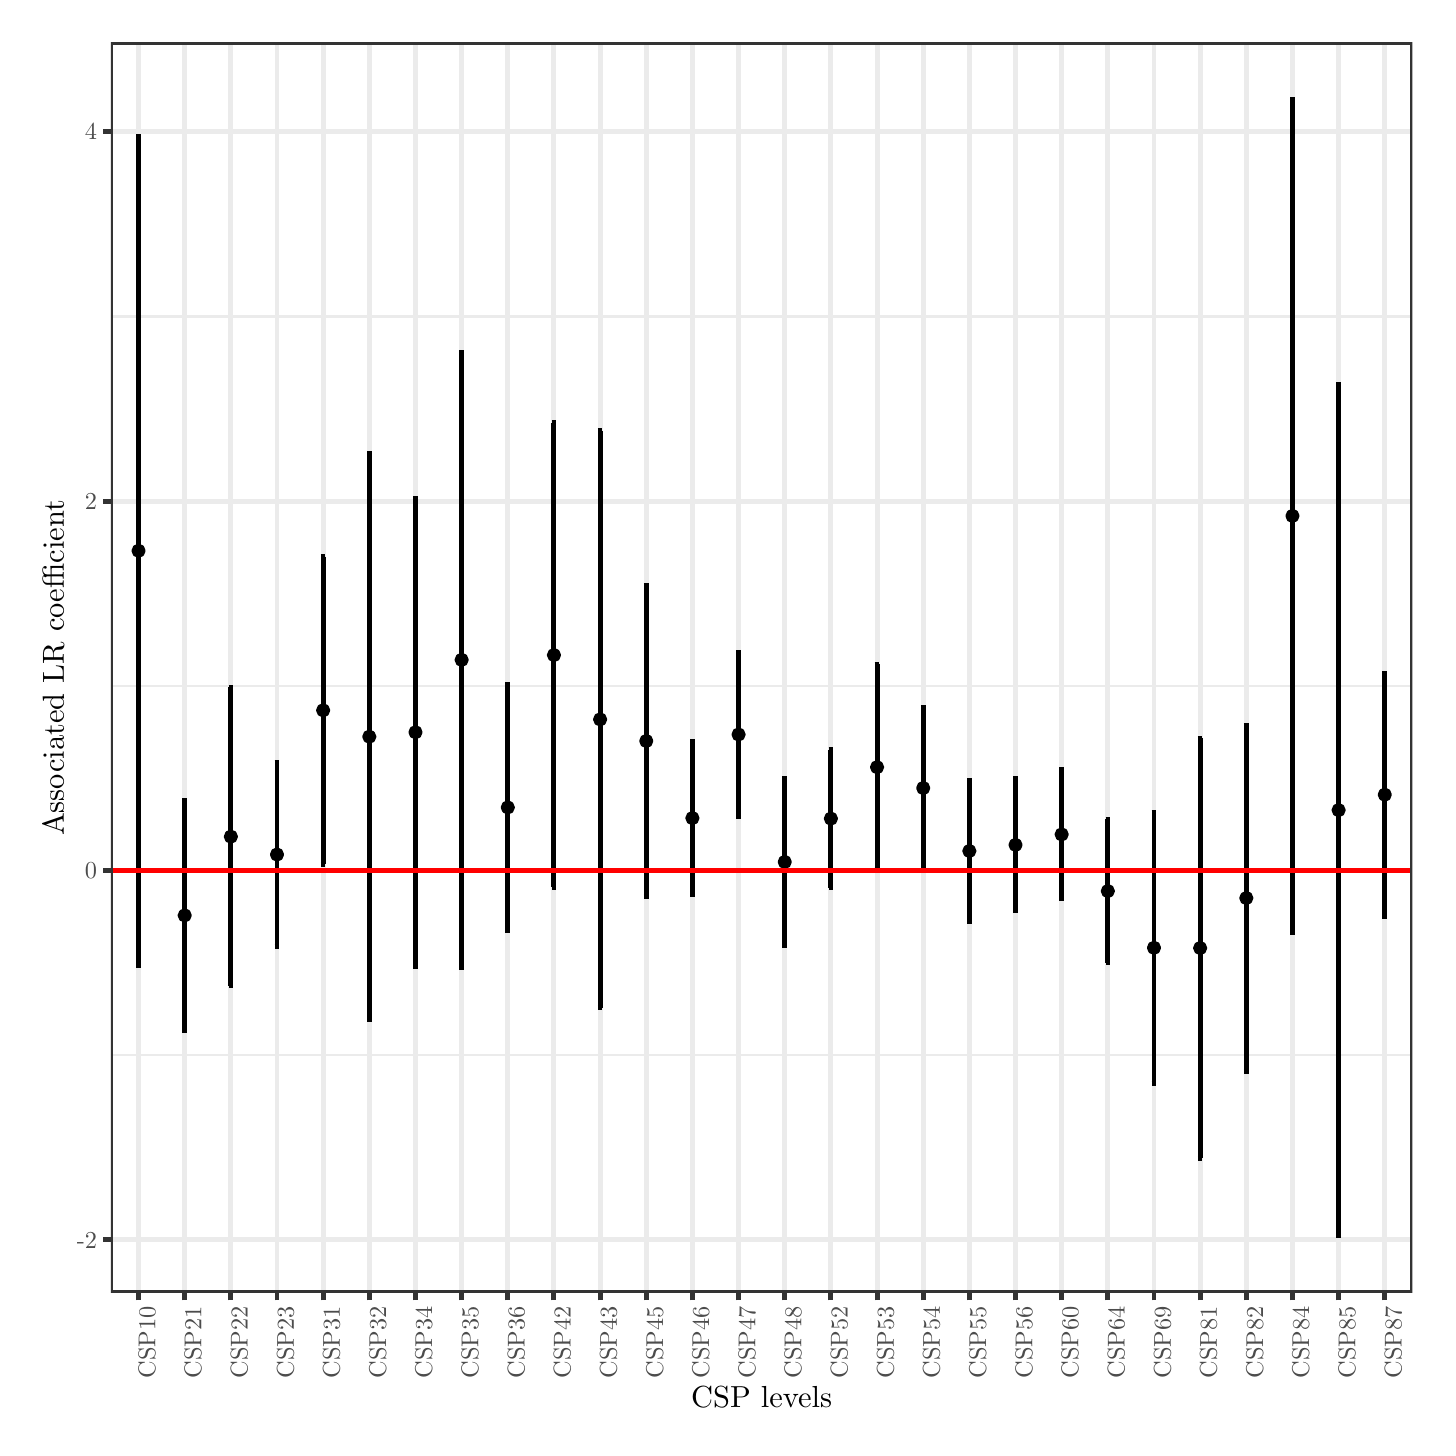
\begin{tikzpicture}[x=1pt,y=1pt]
\definecolor{fillColor}{RGB}{255,255,255}
\path[use as bounding box,fill=fillColor,fill opacity=0.00] (0,0) rectangle (505.89,505.89);
\begin{scope}
\path[clip] (  0.00,  0.00) rectangle (505.89,505.89);
\definecolor{drawColor}{RGB}{255,255,255}
\definecolor{fillColor}{RGB}{255,255,255}

\path[draw=drawColor,line width= 1.8pt,line join=round,line cap=round,fill=fillColor] (  0.00,  0.00) rectangle (505.89,505.89);
\end{scope}
\begin{scope}
\path[clip] ( 30.05, 48.75) rectangle (500.39,500.39);
\definecolor{fillColor}{RGB}{255,255,255}

\path[fill=fillColor] ( 30.05, 48.75) rectangle (500.39,500.39);
\definecolor{drawColor}{gray}{0.92}

\path[draw=drawColor,line width= 0.9pt,line join=round] ( 30.05,134.58) --
	(500.39,134.58);

\path[draw=drawColor,line width= 0.9pt,line join=round] ( 30.05,268.08) --
	(500.39,268.08);

\path[draw=drawColor,line width= 0.9pt,line join=round] ( 30.05,401.59) --
	(500.39,401.59);

\path[draw=drawColor,line width= 1.8pt,line join=round] ( 30.05, 67.82) --
	(500.39, 67.82);

\path[draw=drawColor,line width= 1.8pt,line join=round] ( 30.05,201.33) --
	(500.39,201.33);

\path[draw=drawColor,line width= 1.8pt,line join=round] ( 30.05,334.84) --
	(500.39,334.84);

\path[draw=drawColor,line width= 1.8pt,line join=round] ( 30.05,468.35) --
	(500.39,468.35);

\path[draw=drawColor,line width= 1.8pt,line join=round] ( 40.06, 48.75) --
	( 40.06,500.39);

\path[draw=drawColor,line width= 1.8pt,line join=round] ( 56.74, 48.75) --
	( 56.74,500.39);

\path[draw=drawColor,line width= 1.8pt,line join=round] ( 73.42, 48.75) --
	( 73.42,500.39);

\path[draw=drawColor,line width= 1.8pt,line join=round] ( 90.09, 48.75) --
	( 90.09,500.39);

\path[draw=drawColor,line width= 1.8pt,line join=round] (106.77, 48.75) --
	(106.77,500.39);

\path[draw=drawColor,line width= 1.8pt,line join=round] (123.45, 48.75) --
	(123.45,500.39);

\path[draw=drawColor,line width= 1.8pt,line join=round] (140.13, 48.75) --
	(140.13,500.39);

\path[draw=drawColor,line width= 1.8pt,line join=round] (156.81, 48.75) --
	(156.81,500.39);

\path[draw=drawColor,line width= 1.8pt,line join=round] (173.49, 48.75) --
	(173.49,500.39);

\path[draw=drawColor,line width= 1.8pt,line join=round] (190.17, 48.75) --
	(190.17,500.39);

\path[draw=drawColor,line width= 1.8pt,line join=round] (206.85, 48.75) --
	(206.85,500.39);

\path[draw=drawColor,line width= 1.8pt,line join=round] (223.52, 48.75) --
	(223.52,500.39);

\path[draw=drawColor,line width= 1.8pt,line join=round] (240.20, 48.75) --
	(240.20,500.39);

\path[draw=drawColor,line width= 1.8pt,line join=round] (256.88, 48.75) --
	(256.88,500.39);

\path[draw=drawColor,line width= 1.8pt,line join=round] (273.56, 48.75) --
	(273.56,500.39);

\path[draw=drawColor,line width= 1.8pt,line join=round] (290.24, 48.75) --
	(290.24,500.39);

\path[draw=drawColor,line width= 1.8pt,line join=round] (306.92, 48.75) --
	(306.92,500.39);

\path[draw=drawColor,line width= 1.8pt,line join=round] (323.60, 48.75) --
	(323.60,500.39);

\path[draw=drawColor,line width= 1.8pt,line join=round] (340.27, 48.75) --
	(340.27,500.39);

\path[draw=drawColor,line width= 1.8pt,line join=round] (356.95, 48.75) --
	(356.95,500.39);

\path[draw=drawColor,line width= 1.8pt,line join=round] (373.63, 48.75) --
	(373.63,500.39);

\path[draw=drawColor,line width= 1.8pt,line join=round] (390.31, 48.75) --
	(390.31,500.39);

\path[draw=drawColor,line width= 1.8pt,line join=round] (406.99, 48.75) --
	(406.99,500.39);

\path[draw=drawColor,line width= 1.8pt,line join=round] (423.67, 48.75) --
	(423.67,500.39);

\path[draw=drawColor,line width= 1.8pt,line join=round] (440.35, 48.75) --
	(440.35,500.39);

\path[draw=drawColor,line width= 1.8pt,line join=round] (457.03, 48.75) --
	(457.03,500.39);

\path[draw=drawColor,line width= 1.8pt,line join=round] (473.70, 48.75) --
	(473.70,500.39);

\path[draw=drawColor,line width= 1.8pt,line join=round] (490.38, 48.75) --
	(490.38,500.39);
\definecolor{drawColor}{RGB}{0,0,0}

\path[draw=drawColor,line width= 1.8pt,line join=round] (239.37,247.82) --
	(241.04,247.82);

\path[draw=drawColor,line width= 1.8pt,line join=round] (240.20,247.82) --
	(240.20,192.71);

\path[draw=drawColor,line width= 1.8pt,line join=round] (239.37,192.71) --
	(241.04,192.71);

\path[draw=drawColor,line width= 1.8pt,line join=round] (356.12,234.41) --
	(357.79,234.41);

\path[draw=drawColor,line width= 1.8pt,line join=round] (356.95,234.41) --
	(356.95,186.76);

\path[draw=drawColor,line width= 1.8pt,line join=round] (356.12,186.76) --
	(357.79,186.76);

\path[draw=drawColor,line width= 1.8pt,line join=round] (105.94,314.77) --
	(107.61,314.77);

\path[draw=drawColor,line width= 1.8pt,line join=round] (106.77,314.77) --
	(106.77,203.67);

\path[draw=drawColor,line width= 1.8pt,line join=round] (105.94,203.67) --
	(107.61,203.67);

\path[draw=drawColor,line width= 1.8pt,line join=round] (372.80,237.67) --
	(374.47,237.67);

\path[draw=drawColor,line width= 1.8pt,line join=round] (373.63,237.67) --
	(373.63,191.07);

\path[draw=drawColor,line width= 1.8pt,line join=round] (372.80,191.07) --
	(374.47,191.07);

\path[draw=drawColor,line width= 1.8pt,line join=round] (339.44,233.68) --
	(341.11,233.68);

\path[draw=drawColor,line width= 1.8pt,line join=round] (340.27,233.68) --
	(340.27,183.07);

\path[draw=drawColor,line width= 1.8pt,line join=round] (339.44,183.07) --
	(341.11,183.07);

\path[draw=drawColor,line width= 1.8pt,line join=round] (172.65,268.58) --
	(174.32,268.58);

\path[draw=drawColor,line width= 1.8pt,line join=round] (173.49,268.58) --
	(173.49,179.67);

\path[draw=drawColor,line width= 1.8pt,line join=round] (172.65,179.67) --
	(174.32,179.67);

\path[draw=drawColor,line width= 1.8pt,line join=round] (439.51,253.90) --
	(441.18,253.90);

\path[draw=drawColor,line width= 1.8pt,line join=round] (440.35,253.90) --
	(440.35,128.85);

\path[draw=drawColor,line width= 1.8pt,line join=round] (439.51,128.85) --
	(441.18,128.85);

\path[draw=drawColor,line width= 1.8pt,line join=round] (289.40,245.02) --
	(291.07,245.02);

\path[draw=drawColor,line width= 1.8pt,line join=round] (290.24,245.02) --
	(290.24,195.15);

\path[draw=drawColor,line width= 1.8pt,line join=round] (289.40,195.15) --
	(291.07,195.15);

\path[draw=drawColor,line width= 1.8pt,line join=round] (256.05,280.02) --
	(257.72,280.02);

\path[draw=drawColor,line width= 1.8pt,line join=round] (256.88,280.02) --
	(256.88,220.93);

\path[draw=drawColor,line width= 1.8pt,line join=round] (256.05,220.93) --
	(257.72,220.93);

\path[draw=drawColor,line width= 1.8pt,line join=round] ( 55.90,226.67) --
	( 57.57,226.67);

\path[draw=drawColor,line width= 1.8pt,line join=round] ( 56.74,226.67) --
	( 56.74,143.54);

\path[draw=drawColor,line width= 1.8pt,line join=round] ( 55.90,143.54) --
	( 57.57,143.54);

\path[draw=drawColor,line width= 1.8pt,line join=round] (306.08,275.80) --
	(307.75,275.80);

\path[draw=drawColor,line width= 1.8pt,line join=round] (306.92,275.80) --
	(306.92,201.53);

\path[draw=drawColor,line width= 1.8pt,line join=round] (306.08,201.53) --
	(307.75,201.53);

\path[draw=drawColor,line width= 1.8pt,line join=round] (322.76,260.22) --
	(324.43,260.22);

\path[draw=drawColor,line width= 1.8pt,line join=round] (323.60,260.22) --
	(323.60,202.05);

\path[draw=drawColor,line width= 1.8pt,line join=round] (322.76,202.05) --
	(324.43,202.05);

\path[draw=drawColor,line width= 1.8pt,line join=round] ( 89.26,240.48) --
	( 90.93,240.48);

\path[draw=drawColor,line width= 1.8pt,line join=round] ( 90.09,240.48) --
	( 90.09,173.73);

\path[draw=drawColor,line width= 1.8pt,line join=round] ( 89.26,173.73) --
	( 90.93,173.73);

\path[draw=drawColor,line width= 1.8pt,line join=round] (422.83,249.20) --
	(424.50,249.20);

\path[draw=drawColor,line width= 1.8pt,line join=round] (423.67,249.20) --
	(423.67, 97.43);

\path[draw=drawColor,line width= 1.8pt,line join=round] (422.83, 97.43) --
	(424.50, 97.43);

\path[draw=drawColor,line width= 1.8pt,line join=round] (272.73,234.60) --
	(274.39,234.60);

\path[draw=drawColor,line width= 1.8pt,line join=round] (273.56,234.60) --
	(273.56,174.25);

\path[draw=drawColor,line width= 1.8pt,line join=round] (272.73,174.25) --
	(274.39,174.25);

\path[draw=drawColor,line width= 1.8pt,line join=round] (139.30,335.85) --
	(140.96,335.85);

\path[draw=drawColor,line width= 1.8pt,line join=round] (140.13,335.85) --
	(140.13,166.73);

\path[draw=drawColor,line width= 1.8pt,line join=round] (139.30,166.73) --
	(140.96,166.73);

\path[draw=drawColor,line width= 1.8pt,line join=round] (389.48,219.90) --
	(391.14,219.90);

\path[draw=drawColor,line width= 1.8pt,line join=round] (390.31,219.90) --
	(390.31,167.91);

\path[draw=drawColor,line width= 1.8pt,line join=round] (389.48,167.91) --
	(391.14,167.91);

\path[draw=drawColor,line width= 1.8pt,line join=round] (189.33,363.13) --
	(191.00,363.13);

\path[draw=drawColor,line width= 1.8pt,line join=round] (190.17,363.13) --
	(190.17,195.23);

\path[draw=drawColor,line width= 1.8pt,line join=round] (189.33,195.23) --
	(191.00,195.23);

\path[draw=drawColor,line width= 1.8pt,line join=round] (122.62,352.06) --
	(124.29,352.06);

\path[draw=drawColor,line width= 1.8pt,line join=round] (123.45,352.06) --
	(123.45,147.31);

\path[draw=drawColor,line width= 1.8pt,line join=round] (122.62,147.31) --
	(124.29,147.31);

\path[draw=drawColor,line width= 1.8pt,line join=round] (206.01,360.21) --
	(207.68,360.21);

\path[draw=drawColor,line width= 1.8pt,line join=round] (206.85,360.21) --
	(206.85,151.65);

\path[draw=drawColor,line width= 1.8pt,line join=round] (206.01,151.65) --
	(207.68,151.65);

\path[draw=drawColor,line width= 1.8pt,line join=round] (222.69,304.30) --
	(224.36,304.30);

\path[draw=drawColor,line width= 1.8pt,line join=round] (223.52,304.30) --
	(223.52,191.96);

\path[draw=drawColor,line width= 1.8pt,line join=round] (222.69,191.96) --
	(224.36,191.96);

\path[draw=drawColor,line width= 1.8pt,line join=round] (406.16,222.39) --
	(407.82,222.39);

\path[draw=drawColor,line width= 1.8pt,line join=round] (406.99,222.39) --
	(406.99,124.41);

\path[draw=drawColor,line width= 1.8pt,line join=round] (406.16,124.41) --
	(407.82,124.41);

\path[draw=drawColor,line width= 1.8pt,line join=round] ( 72.58,267.52) --
	( 74.25,267.52);

\path[draw=drawColor,line width= 1.8pt,line join=round] ( 73.42,267.52) --
	( 73.42,159.62);

\path[draw=drawColor,line width= 1.8pt,line join=round] ( 72.58,159.62) --
	( 74.25,159.62);

\path[draw=drawColor,line width= 1.8pt,line join=round] (155.98,388.62) --
	(157.64,388.62);

\path[draw=drawColor,line width= 1.8pt,line join=round] (156.81,388.62) --
	(156.81,166.28);

\path[draw=drawColor,line width= 1.8pt,line join=round] (155.98,166.28) --
	(157.64,166.28);

\path[draw=drawColor,line width= 1.8pt,line join=round] (456.19,479.86) --
	(457.86,479.86);

\path[draw=drawColor,line width= 1.8pt,line join=round] (457.03,479.86) --
	(457.03,179.07);

\path[draw=drawColor,line width= 1.8pt,line join=round] (456.19,179.07) --
	(457.86,179.07);

\path[draw=drawColor,line width= 1.8pt,line join=round] ( 39.22,466.63) --
	( 40.89,466.63);

\path[draw=drawColor,line width= 1.8pt,line join=round] ( 40.06,466.63) --
	( 40.06,167.09);

\path[draw=drawColor,line width= 1.8pt,line join=round] ( 39.22,167.09) --
	( 40.89,167.09);

\path[draw=drawColor,line width= 1.8pt,line join=round] (489.55,272.67) --
	(491.22,272.67);

\path[draw=drawColor,line width= 1.8pt,line join=round] (490.38,272.67) --
	(490.38,184.79);

\path[draw=drawColor,line width= 1.8pt,line join=round] (489.55,184.79) --
	(491.22,184.79);

\path[draw=drawColor,line width= 1.8pt,line join=round] (472.87,377.02) --
	(474.54,377.02);

\path[draw=drawColor,line width= 1.8pt,line join=round] (473.70,377.02) --
	(473.70, 69.28);

\path[draw=drawColor,line width= 1.8pt,line join=round] (472.87, 69.28) --
	(474.54, 69.28);
\definecolor{fillColor}{RGB}{0,0,0}

\path[draw=drawColor,line width= 1.2pt,line join=round,line cap=round,fill=fillColor] (240.20,220.27) circle (  1.96);

\path[draw=drawColor,line width= 1.2pt,line join=round,line cap=round,fill=fillColor] (356.95,210.59) circle (  1.96);

\path[draw=drawColor,line width= 1.2pt,line join=round,line cap=round,fill=fillColor] (106.77,259.22) circle (  1.96);

\path[draw=drawColor,line width= 1.2pt,line join=round,line cap=round,fill=fillColor] (373.63,214.37) circle (  1.96);

\path[draw=drawColor,line width= 1.2pt,line join=round,line cap=round,fill=fillColor] (340.27,208.38) circle (  1.96);

\path[draw=drawColor,line width= 1.2pt,line join=round,line cap=round,fill=fillColor] (173.49,224.12) circle (  1.96);

\path[draw=drawColor,line width= 1.2pt,line join=round,line cap=round,fill=fillColor] (440.35,191.38) circle (  1.96);

\path[draw=drawColor,line width= 1.2pt,line join=round,line cap=round,fill=fillColor] (290.24,220.09) circle (  1.96);

\path[draw=drawColor,line width= 1.2pt,line join=round,line cap=round,fill=fillColor] (256.88,250.48) circle (  1.96);

\path[draw=drawColor,line width= 1.2pt,line join=round,line cap=round,fill=fillColor] ( 56.74,185.11) circle (  1.96);

\path[draw=drawColor,line width= 1.2pt,line join=round,line cap=round,fill=fillColor] (306.92,238.67) circle (  1.96);

\path[draw=drawColor,line width= 1.2pt,line join=round,line cap=round,fill=fillColor] (323.60,231.13) circle (  1.96);

\path[draw=drawColor,line width= 1.2pt,line join=round,line cap=round,fill=fillColor] ( 90.09,207.10) circle (  1.96);

\path[draw=drawColor,line width= 1.2pt,line join=round,line cap=round,fill=fillColor] (423.67,173.32) circle (  1.96);

\path[draw=drawColor,line width= 1.2pt,line join=round,line cap=round,fill=fillColor] (273.56,204.43) circle (  1.96);

\path[draw=drawColor,line width= 1.2pt,line join=round,line cap=round,fill=fillColor] (140.13,251.29) circle (  1.96);

\path[draw=drawColor,line width= 1.2pt,line join=round,line cap=round,fill=fillColor] (390.31,193.90) circle (  1.96);

\path[draw=drawColor,line width= 1.2pt,line join=round,line cap=round,fill=fillColor] (190.17,279.18) circle (  1.96);

\path[draw=drawColor,line width= 1.2pt,line join=round,line cap=round,fill=fillColor] (123.45,249.69) circle (  1.96);

\path[draw=drawColor,line width= 1.2pt,line join=round,line cap=round,fill=fillColor] (206.85,255.93) circle (  1.96);

\path[draw=drawColor,line width= 1.2pt,line join=round,line cap=round,fill=fillColor] (223.52,248.13) circle (  1.96);

\path[draw=drawColor,line width= 1.2pt,line join=round,line cap=round,fill=fillColor] (406.99,173.40) circle (  1.96);

\path[draw=drawColor,line width= 1.2pt,line join=round,line cap=round,fill=fillColor] ( 73.42,213.57) circle (  1.96);

\path[draw=drawColor,line width= 1.2pt,line join=round,line cap=round,fill=fillColor] (156.81,277.45) circle (  1.96);

\path[draw=drawColor,line width= 1.2pt,line join=round,line cap=round,fill=fillColor] (457.03,329.46) circle (  1.96);

\path[draw=drawColor,line width= 1.2pt,line join=round,line cap=round,fill=fillColor] ( 40.06,316.86) circle (  1.96);

\path[draw=drawColor,line width= 1.2pt,line join=round,line cap=round,fill=fillColor] (490.38,228.73) circle (  1.96);

\path[draw=drawColor,line width= 1.2pt,line join=round,line cap=round,fill=fillColor] (473.70,223.15) circle (  1.96);
\definecolor{drawColor}{RGB}{255,0,0}

\path[draw=drawColor,line width= 1.8pt,line join=round] ( 30.05,201.33) -- (500.39,201.33);
\definecolor{drawColor}{gray}{0.20}

\path[draw=drawColor,line width= 1.8pt,line join=round,line cap=round] ( 30.05, 48.75) rectangle (500.39,500.39);
\end{scope}
\begin{scope}
\path[clip] (  0.00,  0.00) rectangle (505.89,505.89);
\definecolor{drawColor}{gray}{0.30}

\node[text=drawColor,anchor=base east,inner sep=0pt, outer sep=0pt, scale=  0.88] at ( 25.10, 64.79) {-2};

\node[text=drawColor,anchor=base east,inner sep=0pt, outer sep=0pt, scale=  0.88] at ( 25.10,198.30) {0};

\node[text=drawColor,anchor=base east,inner sep=0pt, outer sep=0pt, scale=  0.88] at ( 25.10,331.81) {2};

\node[text=drawColor,anchor=base east,inner sep=0pt, outer sep=0pt, scale=  0.88] at ( 25.10,465.32) {4};
\end{scope}
\begin{scope}
\path[clip] (  0.00,  0.00) rectangle (505.89,505.89);
\definecolor{drawColor}{gray}{0.20}

\path[draw=drawColor,line width= 1.8pt,line join=round] ( 27.30, 67.82) --
	( 30.05, 67.82);

\path[draw=drawColor,line width= 1.8pt,line join=round] ( 27.30,201.33) --
	( 30.05,201.33);

\path[draw=drawColor,line width= 1.8pt,line join=round] ( 27.30,334.84) --
	( 30.05,334.84);

\path[draw=drawColor,line width= 1.8pt,line join=round] ( 27.30,468.35) --
	( 30.05,468.35);
\end{scope}
\begin{scope}
\path[clip] (  0.00,  0.00) rectangle (505.89,505.89);
\definecolor{drawColor}{gray}{0.20}

\path[draw=drawColor,line width= 1.8pt,line join=round] ( 40.06, 46.00) --
	( 40.06, 48.75);

\path[draw=drawColor,line width= 1.8pt,line join=round] ( 56.74, 46.00) --
	( 56.74, 48.75);

\path[draw=drawColor,line width= 1.8pt,line join=round] ( 73.42, 46.00) --
	( 73.42, 48.75);

\path[draw=drawColor,line width= 1.8pt,line join=round] ( 90.09, 46.00) --
	( 90.09, 48.75);

\path[draw=drawColor,line width= 1.8pt,line join=round] (106.77, 46.00) --
	(106.77, 48.75);

\path[draw=drawColor,line width= 1.8pt,line join=round] (123.45, 46.00) --
	(123.45, 48.75);

\path[draw=drawColor,line width= 1.8pt,line join=round] (140.13, 46.00) --
	(140.13, 48.75);

\path[draw=drawColor,line width= 1.8pt,line join=round] (156.81, 46.00) --
	(156.81, 48.75);

\path[draw=drawColor,line width= 1.8pt,line join=round] (173.49, 46.00) --
	(173.49, 48.75);

\path[draw=drawColor,line width= 1.8pt,line join=round] (190.17, 46.00) --
	(190.17, 48.75);

\path[draw=drawColor,line width= 1.8pt,line join=round] (206.85, 46.00) --
	(206.85, 48.75);

\path[draw=drawColor,line width= 1.8pt,line join=round] (223.52, 46.00) --
	(223.52, 48.75);

\path[draw=drawColor,line width= 1.8pt,line join=round] (240.20, 46.00) --
	(240.20, 48.75);

\path[draw=drawColor,line width= 1.8pt,line join=round] (256.88, 46.00) --
	(256.88, 48.75);

\path[draw=drawColor,line width= 1.8pt,line join=round] (273.56, 46.00) --
	(273.56, 48.75);

\path[draw=drawColor,line width= 1.8pt,line join=round] (290.24, 46.00) --
	(290.24, 48.75);

\path[draw=drawColor,line width= 1.8pt,line join=round] (306.92, 46.00) --
	(306.92, 48.75);

\path[draw=drawColor,line width= 1.8pt,line join=round] (323.60, 46.00) --
	(323.60, 48.75);

\path[draw=drawColor,line width= 1.8pt,line join=round] (340.27, 46.00) --
	(340.27, 48.75);

\path[draw=drawColor,line width= 1.8pt,line join=round] (356.95, 46.00) --
	(356.95, 48.75);

\path[draw=drawColor,line width= 1.8pt,line join=round] (373.63, 46.00) --
	(373.63, 48.75);

\path[draw=drawColor,line width= 1.8pt,line join=round] (390.31, 46.00) --
	(390.31, 48.75);

\path[draw=drawColor,line width= 1.8pt,line join=round] (406.99, 46.00) --
	(406.99, 48.75);

\path[draw=drawColor,line width= 1.8pt,line join=round] (423.67, 46.00) --
	(423.67, 48.75);

\path[draw=drawColor,line width= 1.8pt,line join=round] (440.35, 46.00) --
	(440.35, 48.75);

\path[draw=drawColor,line width= 1.8pt,line join=round] (457.03, 46.00) --
	(457.03, 48.75);

\path[draw=drawColor,line width= 1.8pt,line join=round] (473.70, 46.00) --
	(473.70, 48.75);

\path[draw=drawColor,line width= 1.8pt,line join=round] (490.38, 46.00) --
	(490.38, 48.75);
\end{scope}
\begin{scope}
\path[clip] (  0.00,  0.00) rectangle (505.89,505.89);
\definecolor{drawColor}{gray}{0.30}

\node[text=drawColor,rotate= 90.00,anchor=base east,inner sep=0pt, outer sep=0pt, scale=  0.88] at ( 46.12, 43.80) {CSP10};

\node[text=drawColor,rotate= 90.00,anchor=base east,inner sep=0pt, outer sep=0pt, scale=  0.88] at ( 62.80, 43.80) {CSP21};

\node[text=drawColor,rotate= 90.00,anchor=base east,inner sep=0pt, outer sep=0pt, scale=  0.88] at ( 79.48, 43.80) {CSP22};

\node[text=drawColor,rotate= 90.00,anchor=base east,inner sep=0pt, outer sep=0pt, scale=  0.88] at ( 96.16, 43.80) {CSP23};

\node[text=drawColor,rotate= 90.00,anchor=base east,inner sep=0pt, outer sep=0pt, scale=  0.88] at (112.83, 43.80) {CSP31};

\node[text=drawColor,rotate= 90.00,anchor=base east,inner sep=0pt, outer sep=0pt, scale=  0.88] at (129.51, 43.80) {CSP32};

\node[text=drawColor,rotate= 90.00,anchor=base east,inner sep=0pt, outer sep=0pt, scale=  0.88] at (146.19, 43.80) {CSP34};

\node[text=drawColor,rotate= 90.00,anchor=base east,inner sep=0pt, outer sep=0pt, scale=  0.88] at (162.87, 43.80) {CSP35};

\node[text=drawColor,rotate= 90.00,anchor=base east,inner sep=0pt, outer sep=0pt, scale=  0.88] at (179.55, 43.80) {CSP36};

\node[text=drawColor,rotate= 90.00,anchor=base east,inner sep=0pt, outer sep=0pt, scale=  0.88] at (196.23, 43.80) {CSP42};

\node[text=drawColor,rotate= 90.00,anchor=base east,inner sep=0pt, outer sep=0pt, scale=  0.88] at (212.91, 43.80) {CSP43};

\node[text=drawColor,rotate= 90.00,anchor=base east,inner sep=0pt, outer sep=0pt, scale=  0.88] at (229.58, 43.80) {CSP45};

\node[text=drawColor,rotate= 90.00,anchor=base east,inner sep=0pt, outer sep=0pt, scale=  0.88] at (246.26, 43.80) {CSP46};

\node[text=drawColor,rotate= 90.00,anchor=base east,inner sep=0pt, outer sep=0pt, scale=  0.88] at (262.94, 43.80) {CSP47};

\node[text=drawColor,rotate= 90.00,anchor=base east,inner sep=0pt, outer sep=0pt, scale=  0.88] at (279.62, 43.80) {CSP48};

\node[text=drawColor,rotate= 90.00,anchor=base east,inner sep=0pt, outer sep=0pt, scale=  0.88] at (296.30, 43.80) {CSP52};

\node[text=drawColor,rotate= 90.00,anchor=base east,inner sep=0pt, outer sep=0pt, scale=  0.88] at (312.98, 43.80) {CSP53};

\node[text=drawColor,rotate= 90.00,anchor=base east,inner sep=0pt, outer sep=0pt, scale=  0.88] at (329.66, 43.80) {CSP54};

\node[text=drawColor,rotate= 90.00,anchor=base east,inner sep=0pt, outer sep=0pt, scale=  0.88] at (346.34, 43.80) {CSP55};

\node[text=drawColor,rotate= 90.00,anchor=base east,inner sep=0pt, outer sep=0pt, scale=  0.88] at (363.01, 43.80) {CSP56};

\node[text=drawColor,rotate= 90.00,anchor=base east,inner sep=0pt, outer sep=0pt, scale=  0.88] at (379.69, 43.80) {CSP60};

\node[text=drawColor,rotate= 90.00,anchor=base east,inner sep=0pt, outer sep=0pt, scale=  0.88] at (396.37, 43.80) {CSP64};

\node[text=drawColor,rotate= 90.00,anchor=base east,inner sep=0pt, outer sep=0pt, scale=  0.88] at (413.05, 43.80) {CSP69};

\node[text=drawColor,rotate= 90.00,anchor=base east,inner sep=0pt, outer sep=0pt, scale=  0.88] at (429.73, 43.80) {CSP81};

\node[text=drawColor,rotate= 90.00,anchor=base east,inner sep=0pt, outer sep=0pt, scale=  0.88] at (446.41, 43.80) {CSP82};

\node[text=drawColor,rotate= 90.00,anchor=base east,inner sep=0pt, outer sep=0pt, scale=  0.88] at (463.09, 43.80) {CSP84};

\node[text=drawColor,rotate= 90.00,anchor=base east,inner sep=0pt, outer sep=0pt, scale=  0.88] at (479.76, 43.80) {CSP85};

\node[text=drawColor,rotate= 90.00,anchor=base east,inner sep=0pt, outer sep=0pt, scale=  0.88] at (496.44, 43.80) {CSP87};
\end{scope}
\begin{scope}
\path[clip] (  0.00,  0.00) rectangle (505.89,505.89);
\definecolor{drawColor}{RGB}{0,0,0}

\node[text=drawColor,anchor=base,inner sep=0pt, outer sep=0pt, scale=  1.10] at (265.22,  7.44) {CSP levels};
\end{scope}
\begin{scope}
\path[clip] (  0.00,  0.00) rectangle (505.89,505.89);
\definecolor{drawColor}{RGB}{0,0,0}

\node[text=drawColor,rotate= 90.00,anchor=base,inner sep=0pt, outer sep=0pt, scale=  1.10] at ( 13.08,274.57) {Associated LR coefficient};
\end{scope}
\end{tikzpicture}
}
\caption{Having a lot of levels means having lots of coefficients, few of which are significant.}
\label{fig:csp_estim}
\end{subfigure}
\begin{subfigure}[t]{0.5\textwidth}
\centering \resizebox{\textwidth}{!}{% Created by tikzDevice version 0.12 on 2019-03-11 09:44:28
% !TEX encoding = UTF-8 Unicode
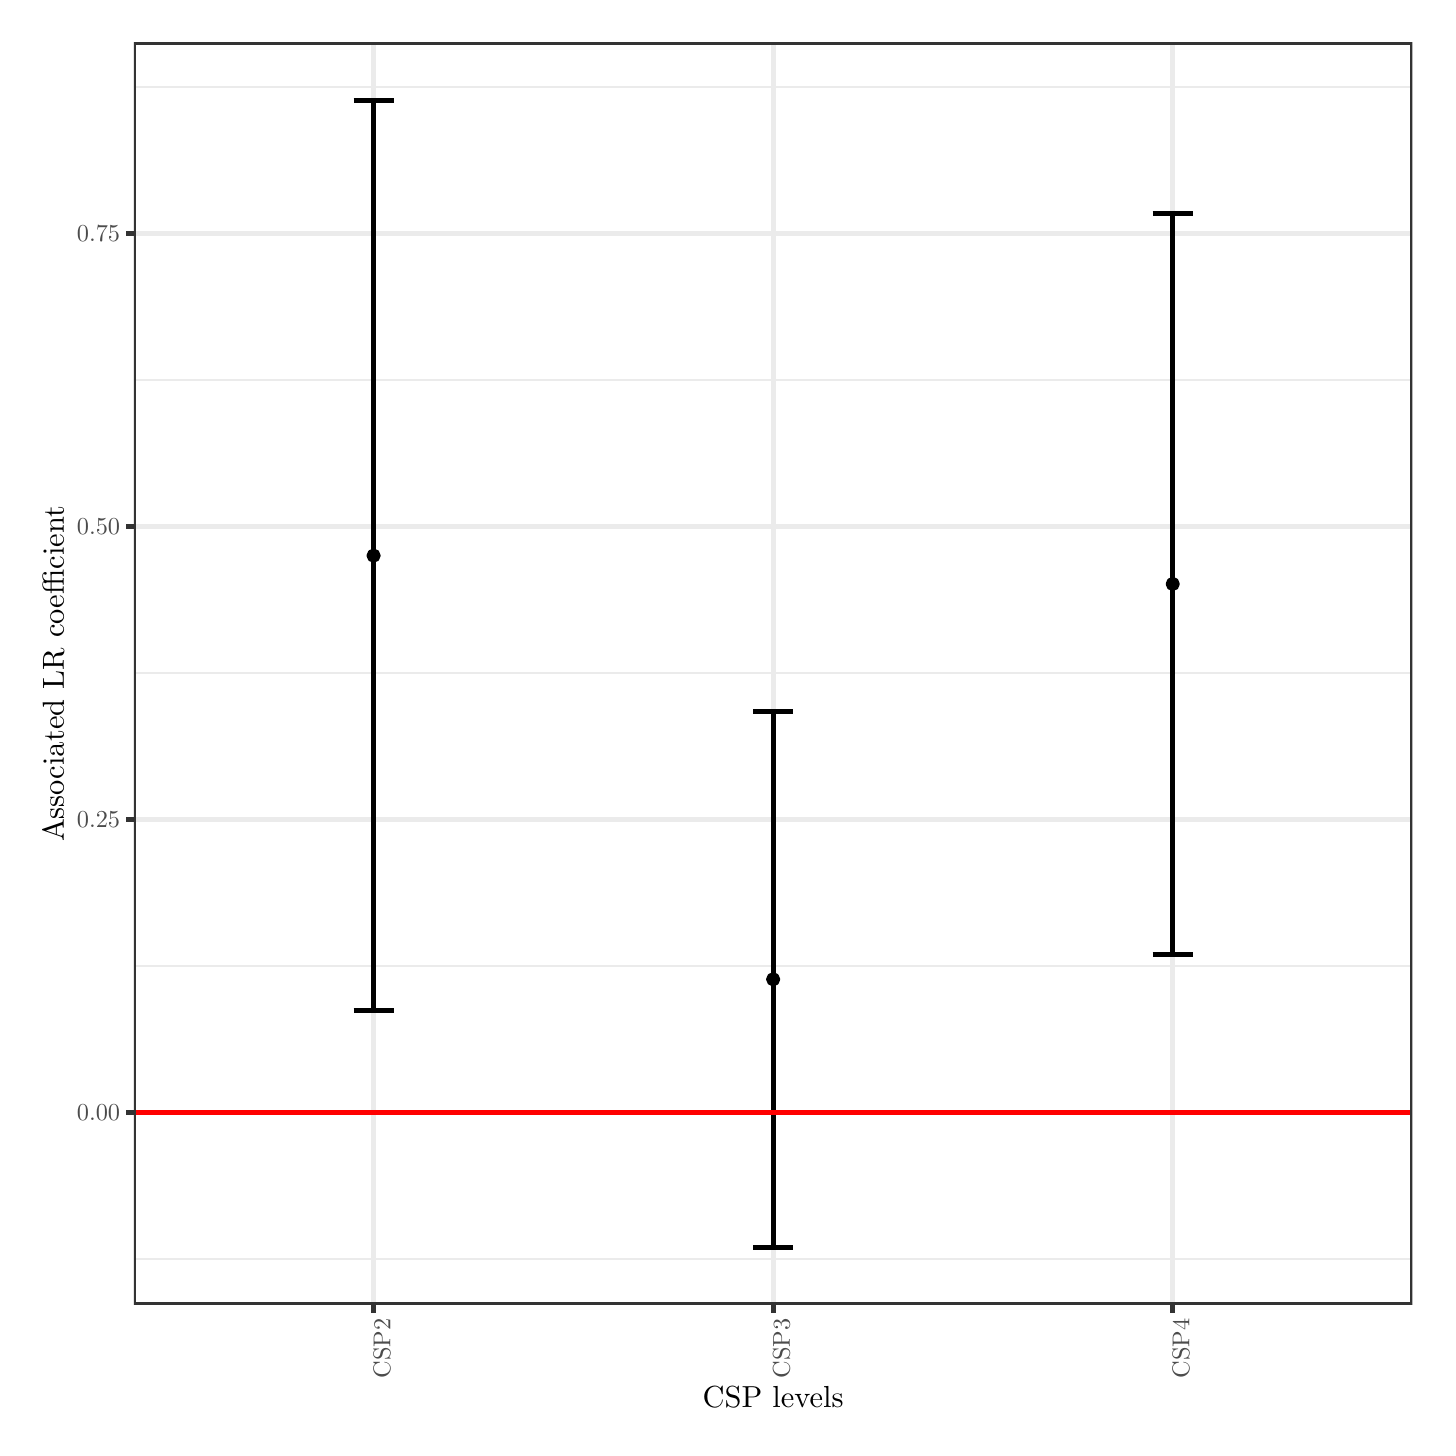
\begin{tikzpicture}[x=1pt,y=1pt]
\definecolor{fillColor}{RGB}{255,255,255}
\path[use as bounding box,fill=fillColor,fill opacity=0.00] (0,0) rectangle (505.89,505.89);
\begin{scope}
\path[clip] (  0.00,  0.00) rectangle (505.89,505.89);
\definecolor{drawColor}{RGB}{255,255,255}
\definecolor{fillColor}{RGB}{255,255,255}

\path[draw=drawColor,line width= 1.8pt,line join=round,line cap=round,fill=fillColor] (  0.00,  0.00) rectangle (505.89,505.89);
\end{scope}
\begin{scope}
\path[clip] ( 38.36, 44.35) rectangle (500.39,500.39);
\definecolor{fillColor}{RGB}{255,255,255}

\path[fill=fillColor] ( 38.36, 44.35) rectangle (500.39,500.39);
\definecolor{drawColor}{gray}{0.92}

\path[draw=drawColor,line width= 0.9pt,line join=round] ( 38.36, 60.90) --
	(500.39, 60.90);

\path[draw=drawColor,line width= 0.9pt,line join=round] ( 38.36,166.79) --
	(500.39,166.79);

\path[draw=drawColor,line width= 0.9pt,line join=round] ( 38.36,272.69) --
	(500.39,272.69);

\path[draw=drawColor,line width= 0.9pt,line join=round] ( 38.36,378.58) --
	(500.39,378.58);

\path[draw=drawColor,line width= 0.9pt,line join=round] ( 38.36,484.48) --
	(500.39,484.48);

\path[draw=drawColor,line width= 1.8pt,line join=round] ( 38.36,113.85) --
	(500.39,113.85);

\path[draw=drawColor,line width= 1.8pt,line join=round] ( 38.36,219.74) --
	(500.39,219.74);

\path[draw=drawColor,line width= 1.8pt,line join=round] ( 38.36,325.64) --
	(500.39,325.64);

\path[draw=drawColor,line width= 1.8pt,line join=round] ( 38.36,431.53) --
	(500.39,431.53);

\path[draw=drawColor,line width= 1.8pt,line join=round] (124.99, 44.35) --
	(124.99,500.39);

\path[draw=drawColor,line width= 1.8pt,line join=round] (269.38, 44.35) --
	(269.38,500.39);

\path[draw=drawColor,line width= 1.8pt,line join=round] (413.76, 44.35) --
	(413.76,500.39);
\definecolor{drawColor}{RGB}{0,0,0}

\path[draw=drawColor,line width= 1.8pt,line join=round] (117.77,479.66) --
	(132.21,479.66);

\path[draw=drawColor,line width= 1.8pt,line join=round] (124.99,479.66) --
	(124.99,150.57);

\path[draw=drawColor,line width= 1.8pt,line join=round] (117.77,150.57) --
	(132.21,150.57);

\path[draw=drawColor,line width= 1.8pt,line join=round] (262.16,258.96) --
	(276.59,258.96);

\path[draw=drawColor,line width= 1.8pt,line join=round] (269.38,258.96) --
	(269.38, 65.08);

\path[draw=drawColor,line width= 1.8pt,line join=round] (262.16, 65.08) --
	(276.59, 65.08);

\path[draw=drawColor,line width= 1.8pt,line join=round] (406.54,438.77) --
	(420.98,438.77);

\path[draw=drawColor,line width= 1.8pt,line join=round] (413.76,438.77) --
	(413.76,170.98);

\path[draw=drawColor,line width= 1.8pt,line join=round] (406.54,170.98) --
	(420.98,170.98);
\definecolor{fillColor}{RGB}{0,0,0}

\path[draw=drawColor,line width= 1.2pt,line join=round,line cap=round,fill=fillColor] (124.99,315.11) circle (  1.96);

\path[draw=drawColor,line width= 1.2pt,line join=round,line cap=round,fill=fillColor] (269.38,162.02) circle (  1.96);

\path[draw=drawColor,line width= 1.2pt,line join=round,line cap=round,fill=fillColor] (413.76,304.87) circle (  1.96);
\definecolor{drawColor}{RGB}{255,0,0}

\path[draw=drawColor,line width= 1.8pt,line join=round] ( 38.36,113.85) -- (500.39,113.85);
\definecolor{drawColor}{gray}{0.20}

\path[draw=drawColor,line width= 1.8pt,line join=round,line cap=round] ( 38.36, 44.35) rectangle (500.39,500.39);
\end{scope}
\begin{scope}
\path[clip] (  0.00,  0.00) rectangle (505.89,505.89);
\definecolor{drawColor}{gray}{0.30}

\node[text=drawColor,anchor=base east,inner sep=0pt, outer sep=0pt, scale=  0.88] at ( 33.41,110.82) {0.00};

\node[text=drawColor,anchor=base east,inner sep=0pt, outer sep=0pt, scale=  0.88] at ( 33.41,216.71) {0.25};

\node[text=drawColor,anchor=base east,inner sep=0pt, outer sep=0pt, scale=  0.88] at ( 33.41,322.61) {0.50};

\node[text=drawColor,anchor=base east,inner sep=0pt, outer sep=0pt, scale=  0.88] at ( 33.41,428.50) {0.75};
\end{scope}
\begin{scope}
\path[clip] (  0.00,  0.00) rectangle (505.89,505.89);
\definecolor{drawColor}{gray}{0.20}

\path[draw=drawColor,line width= 1.8pt,line join=round] ( 35.61,113.85) --
	( 38.36,113.85);

\path[draw=drawColor,line width= 1.8pt,line join=round] ( 35.61,219.74) --
	( 38.36,219.74);

\path[draw=drawColor,line width= 1.8pt,line join=round] ( 35.61,325.64) --
	( 38.36,325.64);

\path[draw=drawColor,line width= 1.8pt,line join=round] ( 35.61,431.53) --
	( 38.36,431.53);
\end{scope}
\begin{scope}
\path[clip] (  0.00,  0.00) rectangle (505.89,505.89);
\definecolor{drawColor}{gray}{0.20}

\path[draw=drawColor,line width= 1.8pt,line join=round] (124.99, 41.60) --
	(124.99, 44.35);

\path[draw=drawColor,line width= 1.8pt,line join=round] (269.38, 41.60) --
	(269.38, 44.35);

\path[draw=drawColor,line width= 1.8pt,line join=round] (413.76, 41.60) --
	(413.76, 44.35);
\end{scope}
\begin{scope}
\path[clip] (  0.00,  0.00) rectangle (505.89,505.89);
\definecolor{drawColor}{gray}{0.30}

\node[text=drawColor,rotate= 90.00,anchor=base east,inner sep=0pt, outer sep=0pt, scale=  0.88] at (131.05, 39.40) {CSP2};

\node[text=drawColor,rotate= 90.00,anchor=base east,inner sep=0pt, outer sep=0pt, scale=  0.88] at (275.44, 39.40) {CSP3};

\node[text=drawColor,rotate= 90.00,anchor=base east,inner sep=0pt, outer sep=0pt, scale=  0.88] at (419.82, 39.40) {CSP4};
\end{scope}
\begin{scope}
\path[clip] (  0.00,  0.00) rectangle (505.89,505.89);
\definecolor{drawColor}{RGB}{0,0,0}

\node[text=drawColor,anchor=base,inner sep=0pt, outer sep=0pt, scale=  1.10] at (269.38,  7.44) {CSP levels};
\end{scope}
\begin{scope}
\path[clip] (  0.00,  0.00) rectangle (505.89,505.89);
\definecolor{drawColor}{RGB}{0,0,0}

\node[text=drawColor,rotate= 90.00,anchor=base,inner sep=0pt, outer sep=0pt, scale=  1.10] at ( 13.08,272.37) {Associated LR coefficient};
\end{scope}
\end{tikzpicture}
}
\caption{By grouping levels, fewer coefficients are obtained, which variance is significantly smaller and are thus significant.}
\label{fig:csp_estim_disc}
\end{subfigure}
\caption{\gls{lr} coefficients of the levels of the job of borrowers.}
\label{fig:csp}
\end{figure}

\section{Illustration of the bias-variance quantization tradeoff} \label{sec:bias_variance_quant}
 

The previous section motivated the use of quantization on a practical level. On a theoretical level, at least in terms of probability theory, quantization is equivalent to throwing away information: for continuous features, it is only known that they belong to a certain interval and for categorical features, their granularity among the original levels is lost.

However, two things must appear clearly: first, we are in a ``statistical'' setting, \textit{i.e.}\ finite-dimensional setting, where variance of estimation can play a big role, as was developed in Section~\ref{subsec:gradient}, which partly justifies the need to regroup categorical levels. Second, we are in a predictive setting, with an imposed classification model $p_{\gls{bth}}$. We focus on \gls{lr}, for which continuous features get a single coefficient: their relationship with the logit transform of the probability of an event (bad borrower) is assumed to be linear which can yield model bias. Thus, having several coefficients per feature, which can be achieved with a  variety of techniques (\textit{e.g.}\ splines), can yield a lower model bias (when the true model is not linear, which is generally the case for \textit{Credit Scoring} data) at the cost of increased variance of estimation.

This phenomenon can be very simply captured by a small simulation: in the misspecified model setting, where the logit transform is assumed to stem from a sinusoidal transformation of $\gls{x}$ on $[0;1]$, it can clearly be seen from Figure~\ref{fig:sinus_lin} that a standard linear \gls{lr} performs poorly. Discretizing the feature $\gls{x}$ results, using a very simple unsupervised heuristic named \textit{equal-length} (described in-depth in Appendix~\ref{app1:equal_length}), in good results (\textit{i.e.}\ visually mild bias / low variance) so long as the number of intervals, and subsequently of \gls{lr} coefficients, is low (see Animation on Figure~\ref{fig:anim_sinus} or still on Figure~\ref{fig:sinus_deb}). When the number of intervals gets large, the bias gets low (the sinus is well approximated by the little step functions), but the variance gets bigger (see Animation on Figure~\ref{fig:anim_sinus} or still on Figure~\ref{fig:sinus_fin}).


%\textcolor{red}{décommenter animation}

\begin{figure}[!ht]
\begin{animateinline}[poster=first, controls=all, palindrome, autopause, autoresume, width=\textwidth, height=7cm]{3}
\multiframe{99}{i=2+1}{\input{R_CODE_FIGURES/chapitre4/disc_plot\i.tex}}%
\end{animateinline}
\caption{\label{fig:anim_sinus} Animation of logistic regression fits on data generated by a sinus with a number of discretization steps in the \textit{equal-length} algorithm ranging from 2 to 100.}
\end{figure}

\begin{figure}[!ht]
%\vspace*{-1cm}
\begin{subfigure}[t]{\textwidth}
\centering \resizebox{.8\textwidth}{!}{\input{R_CODE_FIGURES/chapitre4/linear_plot.tex}}
%\vspace*{-1cm}
\caption{\label{fig:sinus_lin} Linear logistic regression (in \textcolor{red}{red}) fit on data generated by a sinus (in \textcolor{green}{green}).}
\end{subfigure}
%\vspace*{-1cm}
\begin{subfigure}[t]{\textwidth}
\centering \resizebox{.8\textwidth}{!}{\input{R_CODE_FIGURES/chapitre4/disc_plot5.tex}}
%\vspace*{-1cm}
\caption{\label{fig:sinus_deb} Logistic regression fit on data generated by a sinus with 5 discretization steps in the \textit{equal-length} algorithm.}
\end{subfigure}
%\vspace*{-1cm}
\begin{subfigure}[t]{\textwidth}
\centering \resizebox{.8\textwidth}{!}{\input{R_CODE_FIGURES/chapitre4/disc_plot100.tex}}
%\vspace*{-1cm}
\caption{\label{fig:sinus_fin} Logistic regression fit on data generated by a sinus with 100 discretization steps in the \textit{equal-length} algorithm.}
\end{subfigure}
\caption{Motivational example: achieving a good bias-variance trade-off.}
\label{fig:sin_trois}
\end{figure}
 
As the number of intervals is directly linked to the number of coefficient, and to a notion of ``complexity'' of the resulting \gls{lr} model, the bias-variance tradeoff (introduced in Chapter~\ref{chap1}) plays a key role in choosing an appropriate step size, and, as will be seen in the next section which was not possible for the simple \textit{equal-length} algorithm, appropriate step locations (hereafter called cutpoints). Again, this can be witnessed visually by looking at a model selection criterion, \textit{e.g.}\ expected Gini on a test set (which was also introduced in Chapter~\ref{chap1}), for different values of the number of intervals on Figure~\ref{fig:bic_sin}: as was visually concluded from Figure~\ref{fig:anim_sinus}, somewhere around 10-15 intervals seem the most satisfactory. Of course, as the model was misspecified, the flexibility brought by discretization was beneficial. The same phenomenon can b ewitnessed for categorical features on Figure~\ref{fig:csp} with real data from \gls{cacf}. On Figure~\ref{fig:csp_estim}, the \gls{lr} coefficients of the raw job types are displayed: none are significant and estimation variance is large. Grouping these levels results in narrower confidence intervals and significant \gls{lr} parameters as can be seen in Figure~\ref{fig:csp_estim_disc}.
%As can be witnessed from Figure~\ref{fig:bic_sin} with a well-specified model (in \textcolor{blue}{blue}). 
We formalize these empirical findings in the next section.



\begin{figure}[!ht]
\centering \resizebox{.8\textwidth}{!}{% Created by tikzDevice version 0.12 on 2019-03-15 11:11:12
% !TEX encoding = UTF-8 Unicode
\begin{tikzpicture}[x=1pt,y=1pt]
\definecolor{fillColor}{RGB}{255,255,255}
\path[use as bounding box,fill=fillColor,fill opacity=0.00] (0,0) rectangle (578.16,231.26);
\begin{scope}
\path[clip] ( 49.20, 61.20) rectangle (552.96,182.06);
\definecolor{drawColor}{RGB}{0,255,0}

\path[draw=drawColor,line width= 0.4pt,line join=round,line cap=round] ( 67.86,177.59) --
	( 72.62, 93.38) --
	( 77.38, 77.21) --
	( 82.14, 70.94) --
	( 86.90, 68.38) --
	( 91.66, 67.09) --
	( 96.42, 67.10) --
	(101.18, 67.43) --
	(105.93, 65.68) --
	(110.69, 68.26) --
	(115.45, 66.76) --
	(120.21, 66.44) --
	(124.97, 66.53) --
	(129.73, 68.14) --
	(134.49, 69.69) --
	(139.25, 71.88) --
	(144.01, 70.50) --
	(148.77, 71.02) --
	(153.53, 71.36) --
	(158.29, 73.59) --
	(163.05, 74.22) --
	(167.81, 74.83) --
	(172.57, 75.02) --
	(177.33, 75.88) --
	(182.09, 77.79) --
	(186.85, 78.37) --
	(191.61, 79.06) --
	(196.37, 79.37) --
	(201.13, 81.28) --
	(205.89, 81.19) --
	(210.65, 82.61) --
	(215.41, 83.76) --
	(220.17, 83.51) --
	(224.93, 85.71) --
	(229.69, 86.14) --
	(234.45, 87.57) --
	(239.20, 88.43) --
	(243.96, 89.23) --
	(248.72, 89.48) --
	(253.48, 90.31) --
	(258.24, 92.56) --
	(263.00, 91.17) --
	(267.76, 93.39) --
	(272.52, 94.73) --
	(277.28, 96.00) --
	(282.04, 96.42) --
	(286.80, 97.60) --
	(291.56, 97.85) --
	(296.32, 98.32) --
	(301.08,101.41) --
	(305.84,101.76) --
	(310.60,102.22) --
	(315.36,103.44) --
	(320.12,103.64) --
	(324.88,104.19) --
	(329.64,104.13) --
	(334.40,107.13) --
	(339.16,108.00) --
	(343.92,109.53) --
	(348.68,109.82) --
	(353.44,110.05) --
	(358.20,111.95) --
	(362.96,112.74) --
	(367.71,112.13) --
	(372.47,115.37) --
	(377.23,115.37) --
	(381.99,115.72) --
	(386.75,117.40) --
	(391.51,118.68) --
	(396.27,118.00) --
	(401.03,119.57) --
	(405.79,120.07) --
	(410.55,121.41) --
	(415.31,122.79) --
	(420.07,124.14) --
	(424.83,124.99) --
	(429.59,125.09) --
	(434.35,124.68) --
	(439.11,127.12) --
	(443.87,128.18) --
	(448.63,129.76) --
	(453.39,131.28) --
	(458.15,130.59) --
	(462.91,132.47) --
	(467.67,131.11) --
	(472.43,133.57) --
	(477.19,135.51) --
	(481.95,133.72) --
	(486.71,137.04) --
	(491.47,138.57) --
	(496.23,138.16) --
	(500.98,138.90) --
	(505.74,137.75) --
	(510.50,142.49) --
	(515.26,141.71) --
	(520.02,142.20) --
	(524.78,142.13) --
	(529.54,143.26) --
	(534.30,143.22);
\end{scope}
\begin{scope}
\path[clip] (  0.00,  0.00) rectangle (578.16,231.26);
\definecolor{drawColor}{RGB}{0,0,0}

\path[draw=drawColor,line width= 0.4pt,line join=round,line cap=round] ( 58.34, 61.20) -- (534.30, 61.20);

\path[draw=drawColor,line width= 0.4pt,line join=round,line cap=round] ( 58.34, 61.20) -- ( 58.34, 55.20);

\path[draw=drawColor,line width= 0.4pt,line join=round,line cap=round] (153.53, 61.20) -- (153.53, 55.20);

\path[draw=drawColor,line width= 0.4pt,line join=round,line cap=round] (248.72, 61.20) -- (248.72, 55.20);

\path[draw=drawColor,line width= 0.4pt,line join=round,line cap=round] (343.92, 61.20) -- (343.92, 55.20);

\path[draw=drawColor,line width= 0.4pt,line join=round,line cap=round] (439.11, 61.20) -- (439.11, 55.20);

\path[draw=drawColor,line width= 0.4pt,line join=round,line cap=round] (534.30, 61.20) -- (534.30, 55.20);

\node[text=drawColor,anchor=base,inner sep=0pt, outer sep=0pt, scale=  1.00] at ( 58.34, 39.60) {0};

\node[text=drawColor,anchor=base,inner sep=0pt, outer sep=0pt, scale=  1.00] at (153.53, 39.60) {20};

\node[text=drawColor,anchor=base,inner sep=0pt, outer sep=0pt, scale=  1.00] at (248.72, 39.60) {40};

\node[text=drawColor,anchor=base,inner sep=0pt, outer sep=0pt, scale=  1.00] at (343.92, 39.60) {60};

\node[text=drawColor,anchor=base,inner sep=0pt, outer sep=0pt, scale=  1.00] at (439.11, 39.60) {80};

\node[text=drawColor,anchor=base,inner sep=0pt, outer sep=0pt, scale=  1.00] at (534.30, 39.60) {100};

\path[draw=drawColor,line width= 0.4pt,line join=round,line cap=round] ( 49.20, 83.18) -- ( 49.20,173.12);

\path[draw=drawColor,line width= 0.4pt,line join=round,line cap=round] ( 49.20, 83.18) -- ( 43.20, 83.18);

\path[draw=drawColor,line width= 0.4pt,line join=round,line cap=round] ( 49.20,105.67) -- ( 43.20,105.67);

\path[draw=drawColor,line width= 0.4pt,line join=round,line cap=round] ( 49.20,128.15) -- ( 43.20,128.15);

\path[draw=drawColor,line width= 0.4pt,line join=round,line cap=round] ( 49.20,150.64) -- ( 43.20,150.64);

\path[draw=drawColor,line width= 0.4pt,line join=round,line cap=round] ( 49.20,173.12) -- ( 43.20,173.12);

\node[text=drawColor,rotate= 90.00,anchor=base,inner sep=0pt, outer sep=0pt, scale=  1.00] at ( 34.80, 83.18) {13000};

\node[text=drawColor,rotate= 90.00,anchor=base,inner sep=0pt, outer sep=0pt, scale=  1.00] at ( 34.80,128.15) {13400};

\node[text=drawColor,rotate= 90.00,anchor=base,inner sep=0pt, outer sep=0pt, scale=  1.00] at ( 34.80,173.12) {13800};

\path[draw=drawColor,line width= 0.4pt,line join=round,line cap=round] ( 49.20, 61.20) --
	(552.96, 61.20) --
	(552.96,182.06) --
	( 49.20,182.06) --
	( 49.20, 61.20);
\end{scope}
\begin{scope}
\path[clip] (  0.00,  0.00) rectangle (578.16,231.26);
\definecolor{drawColor}{RGB}{0,0,0}

\node[text=drawColor,anchor=base,inner sep=0pt, outer sep=0pt, scale=  1.00] at (301.08, 15.60) {Number of bins in \textit{equal-freq}};

\node[text=drawColor,rotate= 90.00,anchor=base,inner sep=0pt, outer sep=0pt, scale=  1.00] at ( 10.80,121.63) {BIC};
\end{scope}
\begin{scope}
\path[clip] ( 49.20, 61.20) rectangle (552.96,182.06);
\definecolor{drawColor}{RGB}{255,0,0}

\path[draw=drawColor,line width= 0.4pt,line join=round,line cap=round] ( 67.86,177.84) --
	( 72.62,177.84) --
	( 77.38,177.84) --
	( 82.14,177.84) --
	( 86.90,177.84) --
	( 91.66,177.84) --
	( 96.42,177.84) --
	(101.18,177.84) --
	(105.93,177.84) --
	(110.69,177.84) --
	(115.45,177.84) --
	(120.21,177.84) --
	(124.97,177.84) --
	(129.73,177.84) --
	(134.49,177.84) --
	(139.25,177.84) --
	(144.01,177.84) --
	(148.77,177.84) --
	(153.53,177.84) --
	(158.29,177.84) --
	(163.05,177.84) --
	(167.81,177.84) --
	(172.57,177.84) --
	(177.33,177.84) --
	(182.09,177.84) --
	(186.85,177.84) --
	(191.61,177.84) --
	(196.37,177.84) --
	(201.13,177.84) --
	(205.89,177.84) --
	(210.65,177.84) --
	(215.41,177.84) --
	(220.17,177.84) --
	(224.93,177.84) --
	(229.69,177.84) --
	(234.45,177.84) --
	(239.20,177.84) --
	(243.96,177.84) --
	(248.72,177.84) --
	(253.48,177.84) --
	(258.24,177.84) --
	(263.00,177.84) --
	(267.76,177.84) --
	(272.52,177.84) --
	(277.28,177.84) --
	(282.04,177.84) --
	(286.80,177.84) --
	(291.56,177.84) --
	(296.32,177.84) --
	(301.08,177.84) --
	(305.84,177.84) --
	(310.60,177.84) --
	(315.36,177.84) --
	(320.12,177.84) --
	(324.88,177.84) --
	(329.64,177.84) --
	(334.40,177.84) --
	(339.16,177.84) --
	(343.92,177.84) --
	(348.68,177.84) --
	(353.44,177.84) --
	(358.20,177.84) --
	(362.96,177.84) --
	(367.71,177.84) --
	(372.47,177.84) --
	(377.23,177.84) --
	(381.99,177.84) --
	(386.75,177.84) --
	(391.51,177.84) --
	(396.27,177.84) --
	(401.03,177.84) --
	(405.79,177.84) --
	(410.55,177.84) --
	(415.31,177.84) --
	(420.07,177.84) --
	(424.83,177.84) --
	(429.59,177.84) --
	(434.35,177.84) --
	(439.11,177.84) --
	(443.87,177.84) --
	(448.63,177.84) --
	(453.39,177.84) --
	(458.15,177.84) --
	(462.91,177.84) --
	(467.67,177.84) --
	(472.43,177.84) --
	(477.19,177.84) --
	(481.95,177.84) --
	(486.71,177.84) --
	(491.47,177.84) --
	(496.23,177.84) --
	(500.98,177.84) --
	(505.74,177.84) --
	(510.50,177.84) --
	(515.26,177.84) --
	(520.02,177.84) --
	(524.78,177.84) --
	(529.54,177.84) --
	(534.30,177.84);
\definecolor{drawColor}{RGB}{0,0,0}

\path[draw=drawColor,line width= 0.4pt,line join=round,line cap=round] (105.93,161.88) rectangle (230.86,125.88);
\definecolor{drawColor}{RGB}{0,255,0}

\path[draw=drawColor,line width= 0.8pt,line join=round,line cap=round] (114.93,149.88) -- (132.93,149.88);
\definecolor{drawColor}{RGB}{255,0,0}

\path[draw=drawColor,line width= 0.8pt,line join=round,line cap=round] (114.93,137.88) -- (132.93,137.88);
\definecolor{drawColor}{RGB}{0,0,0}

\node[text=drawColor,anchor=base west,inner sep=0pt, outer sep=0pt, scale=  1.00] at (141.93,146.44) {Quantized data LR};

\node[text=drawColor,anchor=base west,inner sep=0pt, outer sep=0pt, scale=  1.00] at (141.93,134.44) {Linear LR};
\end{scope}
\end{tikzpicture}
}
\caption{\label{fig:bic_sin} BIC of the resulting logistic regression on quantized data in \textcolor{green}{green} with a varying number of bins in the \textit{equal-length} algorithm and the linear logistic regression Gini in \textcolor{red}{red} (both misspecified).}
\end{figure}


 
\section{Quantization as a combinatorial challenge} \label{sec:model_selection}

\subsection{Quantization: definition}

\paragraph{General principle}

The quantization procedure consists in turning a $d$-dimensional raw vector of continuous and/or categorical features $\gls{bx} = (\gls{x}_1, \ldots, \gls{x}_d)$ into a $d$-dimensional categorical vector \textit{via} a component wise mapping $\q=(\gls{qj})_1^d$:
\[\q(\gls{bx})=(\q_1(\gls{x}_1),\ldots,\q_d(\gls{x}_d)),\]
where each of the $\gls{qj}$'s is a vector of $\gls{mj}$ dummies: 
\begin{align}\label{eq:qj}
& q_{j,h}(\cdot) =  1 \text{ if } \gls{x}_j \in C_{j,h}, 0 \text{ otherwise, } 1 \leq h \leq \gls{mj}, \\
\equiv & \gls{qj}(\cdot) = \gls{ehmj} \nonumber
\end{align}
where $\gls{mj}$ is an integer, $\gls{ehmj}$ is the $h^{\text{th}}$ basis vector of $\gls{R}^{\gls{mj}}$ and the sets $C_{j,h}$ are defined with respect to each feature type as is described just below.
\paragraph{Raw continuous features} If $\gls{x}_j$ is a continuous component of $\gls{bx}$, quantization $\gls{qj}$ has to perform a discretization of $\gls{x}_j$ and the $C_{j,h}$'s, $1 \leq h \leq \gls{mj}$, are contiguous intervals  
\begin{equation}\label{eq:Cjhcont}
C_{j,h}=(c_{j,h-1},c_{j,h}]
\end{equation}
where $c_{j,1},\ldots,c_{j,\gls{mj}-1}$ are increasing numbers called cutpoints, $c_{j,0}=-\infty$, $c_{j,\gls{mj}}=\infty$. For example, the quantization of the unit segment in thirds would be defined as $\gls{mj}=3$, $c_{j,1} = 1/3$, $c_{j,2} = 2/3$ and subsequently $\gls{qj}(0.1) = (1,0,0)$. This is visually exemplified on Figure~\ref{fig:disc_cont}.
\paragraph{Raw categorical features} If $\gls{x}_j$ is a categorical component of $\gls{bx}$, quantization $\gls{qj}$ consists in grouping levels of $\gls{x}_j$ and the $C_{j,h}$s form a partition of the set $\gls{NO}$.
%, say $\{1,\ldots,l_j\}$, of levels of $\gls{x}_j$: 
\begin{equation*}
%\bigsqcup_{h=1}^{\gls{mj}}C_{j,h}=\{1,\ldots,\gls{lj}\}.
\bigsqcup_{h=1}^{\gls{mj}}C_{j,h}=\gls{NO}.
\end{equation*}
For example, the grouping of levels encoded as ``1'' and ``2'' would yield $C_{j,1} = \{1,2\}$ such that $\gls{qj}(1) = \gls{qj}(2) = (1,0,\ldots,0)$. Note that it is assumed that there are no empty buckets, \textit{i.e.}\ $\nexists j, h$ s.t.\ $C_{j,h} = \varnothing$ and that there is no overlap, \textit{i.e.}\ $\nexists j,h,h'$ s.t.\ $C_{j,h} \cup C_{j,h'} = \varnothing$. This is visually exemplified on Figure~\ref{fig:disc_disc}.

\begin{figure}[!ht]
\begin{multicols}{2}

\begin{minipage}{0.45\textwidth}
\centering
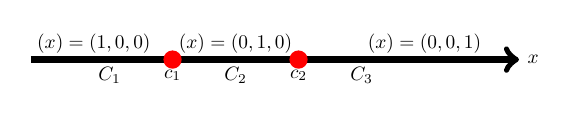
\begin{tikzpicture}[scale=0.2,every node/.style={scale=0.7}]
\draw[->,line width=0.08cm] (-5,0)--(26,0) node[right]{$\gls{x}$};

\node at (0,-1) {$C_1$};
\node at (8,-1) {$C_2$};
\node at (16,-1) {$C_3$};

\node at (4,-1) {$c_1$};
\node at (12,-1) {$c_2$};

\node [red,circle, fill] at (4,0) {};
\node [red,circle, fill] at (12,0) {};

\node at (-1,1) {$\q(x) = (1,0,0)$};
\node at (8,1) {$\q(x) = (0,1,0)$};
\node at (20,1) {$\q(x) = (0,0,1)$};
\end{tikzpicture}
\caption{\label{fig:disc_cont} Quantization (discretization) of a continuous feature.}
\end{minipage}

\columnbreak

\begin{minipage}{0.45\textwidth}
\centering
\begin{tikzpicture}[scale=0.2,every node/.style={scale=0.7}]
\tikzset{vertex/.style = {shape=circle,draw,scale=0.7,minimum size=1cm}}
\tikzset{edge/.style = {->,> = latex'}}

% Boules E^j
\node [vertex] (q1) at (3,2.5) {(1,0)};
\node [vertex] (q2) at (15,2.5) {(0,1)};

% Boules X^J
\node [vertex] (x1) at (-4,0) {0};
\node [vertex] (x2) at (1.8,0) {1};
\node [vertex] (x3) at (9.5,0) {2};
\node [vertex] (x4) at (17,0) {3};
\node [vertex] (x5) at (24,0) {4};

% Labels
\node at (-7,2.5) {$\q(\gls{x})=$};
\node at (-7,0.2) {$\gls{x}=$};

% Flèches
\draw[edge,line width=0.03cm] (x1) to (q1);
\draw[edge,line width=0.03cm] (x3) to (q1);
\draw[edge,line width=0.03cm] (x4) to (q1);
\draw[edge,line width=0.03cm] (x2) to (q2);
\draw[edge,line width=0.03cm] (x5) to (q2);

\end{tikzpicture}
\caption{\label{fig:disc_disc} Quantization (factor levels merging) of categorical feature.}
\end{minipage}
\end{multicols}
\end{figure}


\paragraph{Notations for the quantization family}

In both continuous and categorical cases, keep in mind that $\gls{mj}$ is the dimension of $\gls{qj}$. For notational convenience, the (global) order of the quantization $\q$ is set as 
\[|\q|=\sum_{j=1}^d \gls{mj}.\]
The space where quantizations $\q$ live (resp. $\gls{qj}$) will be denoted by $\gls{bQm}$ in the sequel (resp. $\gls{bQjmj}$), when the number of levels $\gls{bm} = (\gls{mj})_1^d$ is fixed. Since it is not known, the full model space is $\Q = \cup_{m \in \gls{N}_\star^{d}} \gls{bQm}$.

\subparagraph{Equivalence of quantizations} \label{par:equiv}

Let $\q^1$ and $\q^2$ in $\Q$ such that $\q^1 \mathcal{R}_{\gls{T}_n} \q^2 \equiv \forall i,j \; \q^1_j(\gls{xij}) = \q^2_j(\gls{xij})$. See Figure~\ref{fig:equiv} for an example.

\subparagraph{Lemma} Relation $\mathcal{R}_{\gls{T}_n}$ defines an equivalence relation on $\Q$.

\begin{proof}
Relation $\mathcal{R}_{\gls{T}_n}$ is trivially reflexive and symmetric because of the reflexive and symmetric nature of the equality relation in $\gls{R}$: $\forall i,j \; \q^1_j(\gls{xij}) = \q^1_j(\gls{xij})$ and $\forall i,j \; \q^1(\gls{xij}) = \q^2(\gls{xij})$. Similarly, let $\q^3 \in \Q$ such that $\q^1 \mathcal{R}_{\gls{T}_n} \q^3  \equiv \forall i,j \; \q^1_j(\gls{xij}) = \q^3_j(\gls{xij})$. Again, we immediately get $\forall i,j \; \q^2_j(\gls{xij}) = \q^3_j(\gls{xij})$, \textit{i.e.}\ $\q^2 \mathcal{R}_{\gls{T}_n} \q^3$ which proves the transitivity of $\mathcal{R}_{\gls{T}_n}$.
\end{proof}

 \begin{figure}[!ht]
     \centering
     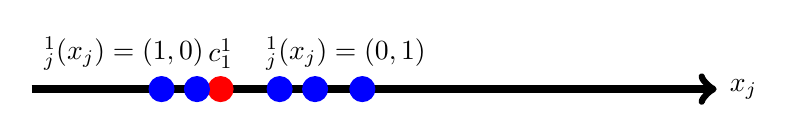
\begin{tikzpicture}[scale=0.3]
 \draw[->,line width=0.1cm] (-5,0)--(24,0) node[right]{$\gls{x}_j$};

 \node [red,circle,fill] at (3,0) {};

 \node [blue,circle, fill] at (0.5,0) {};
 \node [blue,circle, fill] at (2,0) {};

 \node [blue,circle, fill] at (5.5,0) {};
 \node [blue,circle, fill] at (7,0) {};
 \node [blue,circle, fill] at (9,0) {};

 \node at (3,1.5) {$c^1_1$};

 \node at (-1.1,1.5) {$\q^1_j(\gls{x}_j) = (1,0)$};
 \node at (8.3,1.5) {$\q^1_j(\gls{x}_j) = (0,1)$};
 \end{tikzpicture}

 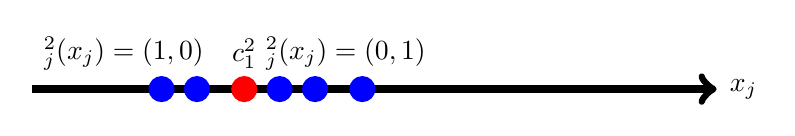
\begin{tikzpicture}[scale=0.3]
 \draw[->,line width=0.1cm] (-5,0)--(24,0) node[right]{$x_j$};

 \node [red,circle,fill] at (4,0) {};

 \node [blue,circle, fill] at (0.5,0) {};
 \node [blue,circle, fill] at (2,0) {};

 \node [blue,circle, fill] at (5.5,0) {};
 \node [blue,circle, fill] at (7,0) {};
 \node [blue,circle, fill] at (9,0) {};

 \node at (4,1.5) {$c^2_1$};

 \node at (-1.1,1.5) {$\q^2_j(x_j) = (1,0)$};
 \node at (8.3,1.5) {$\q^2_j(x_j) = (0,1)$};

 \end{tikzpicture}

     \caption{On the sample $\gls{bbx}$ (blue points), the two discretization functions $\q^1$ and $\q^2$ (which respective unique cutpoint $c^1_1$ and $c^2_1$ are displayed in red) take the same value and are thus equivalent w.r.t. $\mathcal{R}_{\gls{T}_n}$.}
     \label{fig:equiv}
 \end{figure}


\subparagraph{Cardinality of the quantization family in the continuous case} ~\label{par:cardinality}

For a continuous feature $x_j$, let $\gls{qj} \in \gls{bQjmj}$ and cutpoints $\boldsymbol{c}_j$. Without any loss of generality, \textit{i.e.}\ up to a relabelling on individuals $i$, it can be assumed that there are $\gls{mj}+1$ observations $x_{1,j},\dots,x_{\gls{mj}+1,j}$ s.t.\ $x_{1,j} < c_{j,1} < x_{2,j} < \dots < c_{\gls{mj}-1,1} < x_{\gls{mj}+1,j}$. Indeed, if for example there exists $k < \gls{mj} - 1$ s.t.\ $c_{j,k} < \dots < c_{j,\gls{mj}-1}$ and $\max_{1 \leq i \leq n} x_{i,j} < c_{j,k}$, then discretization $\q^{\text{bis}}_j \in \gls{bQj}$ with $k+1$ cutpoints $(-\infty,c_{j,1},\dots,c_{j,k-1},+\infty)$ is equivalent w.r.t.\ $\mathcal{R}_{\gls{T}_n}$ to $\gls{qj}$: $\forall i, \; \gls{qj}(x_{i,j}) = \q^{\text{bis}}_j(x_{i,j})$. A similar proof can be conducted with cutpoints below the minimum of $\gls{bx}_j$ or with several cutpoints in-between consecutive values of the observations. Subsequently, there are $\binom{n-1}{\gls{mj}-1}$ ways to construct $\bm{c}_j$, \textit{i.e.}\ equivalence classes $[\gls{qj}]$ for a fixed $\gls{mj} \leq n$. The number of intervals $\gls{mj}$ can range from $2$ (binarization) to $n$ (each $x_{i,j}$ is in its own interval, thus $\gls{qj}(x_{i,j}) \neq \gls{qj}(x_{i',j})$ for $i \neq i'$), so that the number of admissible discretization of $\gls{bbx}_j$ is $|\gls{bQj}| = \sum_{i=2}^{n}$ ${n-1}\choose{i-1}$. Note that $|\gls{bQj}|$ depends on the number of observations $n$; we shall go back to this property in the following section.


\subparagraph{Cardinality of the quantization family in the categorical case}

For a continuous feature $x_j$, let $\gls{qj} \in \gls{bQj}$ with $\gls{mj}$ groups. The number of re-arrangements of $\gls{lj}$ labelled elements into $\gls{mj}$ unlabelled groups is given by the Stirling number of the second kind $S(\gls{lj},\gls{mj}) = \frac{1}{\gls{mj}!} \sum_{i=0}^{\gls{mj}} (-1)^{\gls{mj}-i} {\gls{mj} \choose i} i^{\gls{lj}}$. As $\gls{mj}$ is unknown and must be searched over the range $\{1,\dots,\gls{lj}\}$. Thus for categorical features, model space $\gls{bQj}$ is also discrete; subsequently, $\Q = \prod_{j=1}^d \gls{bQj}$ is discrete.







\paragraph{Literature review}

The current practice of quantization is prior to any predictive task, thus ignoring its consequences on the final predictive ability. It consists in optimizing a heuristic criterion, often totally unrelated (unsupervised methods) or at least explicitly (supervised methods) to prediction, and mostly univariate (each feature is quantized irrespective of other features' values). The cardinality of the quantization space $\Q$ was calculated explicitely w.r.t.\ $d$, $(\gls{mj})_1^d$ and, for categorical features, $\gls{lj}$: it is huge, so that a greedy approach is intractable and such heuristics are needed, as will be detailed in the next section.
Many algorithms have thus been designed and a review of approximatively 200 discretization strategies, gathering both criteria and related algorithms, can be found in~\cite{ramirez2016data}, preceded by other enlightening review articles such as~\cite{dougherty1995supervised,liu2002discretization}. They classify discretization methods by distinguishing, among other criteria and as said previously, unsupervised and supervised methods ($\bm{y}$ is used to discretize $\gls{bx}$), for which model-specific (assumptions on $p_{\gls{bth}}$) or model-free approaches are distinguished, univariate and multivariate methods (features $\gls{Xnotj} = (X_{1},\ldots,X_{j-1},X_{j+1},\ldots,X_{d})$ may influence the quantization scheme of $\gls{Xj}$) and other criteria as can be seen from Figure~\ref{fig:taxonomy} reproduced from~\cite{ramirez2016data} with permission. For factor levels grouping, We found no such taxonomy, but some discretization methods, \textit{e.g.}\ $\chi^2$ independence test-based methods can be naturally extended to this type of quantization, which is for example what the CHAID algorithm, proposed in~\cite{kass1980exploratory} and applied to each categorical feature, relies on. A simple idea is to use Group LASSO~\cite{meier2008group} which attempts to shrink to zero all coefficients of a categorical feature to avoid situations where a few levels enter the model, which is arguably less interpretable. Another idea would be to use Fused LASSO~\cite{tibshirani2005sparsity}, which seeks to shrink the pairwise absolute difference of selected coefficients, and apply it to all pairs of levels: the levels for which the difference would be shrunk to zero would be grouped. A combination of both approaches would allow both selection and grouping\footnote{See \url{https://stats.stackexchange.com/questions/60100/penalized-methods-for-categorical-data-combining-levels-in-a-factor}}.
For benchmarking purposes, and following results found in the taxonomy of~\cite{ramirez2016data}, we used the MDLP~\cite{fayyad1993multi} discretization method, described in-depth in Appendix~\ref{app1:mdlp}, which is a popular supervised univariate discretization method, and I implemented an extension of the discretization method ChiMerge~\cite{kerber1992chimerge} to categorical features, performing pairwise $\chi^2$ independence tests rather than only pairs of contiguous intervals, which we called ChiCollapse and describe in-depth in Appendix~\ref{app1:chicollapse}. Note that various refinements of ChiMerge have been proposed in the literature, Chi2~\cite{liu1995chi2}, ConMerge~\cite{wang1998concurrent}, ModifiedChi2~\cite{tay2002modified}, and ExtendedChi2~\cite{su2005extended}, which seek to correct for multiple hypothesis testing~\cite{shaffer1995multiple} and automize the choice of the confidence parameter $\alpha$ in the $\chi^2$ tests, but adapting them to categorical features for benchmarking purposes would have been too time-consuming. A similar measure, called Zeta, has been proposed in place of $\chi^2$ in~\cite{ho1997zeta} and subsequent refinement~\cite{ho1998efficient}: it is the classification error achievable by using only two contiguous intervals; if it is low, the two intervals are dissimilar w.r.t.\ the prediction task, if not, they can be merged.

\begin{figure}[!ht]
\includegraphics[width=\textwidth]{figures/chapitre4/taxonomy.PNG}
\caption{Taxonomy of discretization methods.}
\label{fig:taxonomy}
\end{figure}



\subsection{Quantization embedded in a predictive process} \label{subsec:embedding}

In what follows, focus is given to \gls{lr} since it is a requirement from \gls{cacf} but it is applicable to any other supervised (binary) classification model.

\paragraph{Logistic regression on quantized data}

Quantization is a widespread preprocessing step to perform a learning task consisting in predicting, say, a binary variable $\gls{y}\in\{0,1\}$, from a quantized predictor  $\q(\gls{bx})$, through, say, a parametric conditional distribution $p_{\gls{bth}}(\gls{y}|\q(\gls{bx}))$ like \gls{lr}; the whole process can be visually represented as a dependence structure among $\gls{bX}$, its quantization $\bm{Q}$ (which notation as a random variable will be made clearer in Section~\ref{sec:sem}) and the target $\gls{Y}$ on Figure~\ref{fig:dep}. Considering quantized data instead of raw data has a double benefit. First, the quantization order $|\q|$ acts as a tuning parameter for controlling the model's flexibility and thus the bias/variance trade-off of the estimate of the parameter $\gls{bth}$ (or of its predictive accuracy) for a given dataset. This claim becomes clearer with the example of logistic regression I focus on, as a still very popular model for many practitioners. On quantized data, Equation~\eqref{eq:logit} becomes:
\begin{equation}
    \label{eq:reglogq}
\ln \left( \dfrac{p_{\gls{bth}}(1|\q(\gls{bx}))}{1 - p_{\gls{bth}}(1|\q(\gls{bx}))} \right) = \theta_0 + \sum_{j=1}^d \gls{qj}(\gls{x}_j)' \gls{bth}_j,
\end{equation}
where $\gls{bth} = (\theta_{0},(\gls{bth}_j)_1^d) \in \gls{R}^{|\q|+1}$ and $\gls{bth}_j = (\theta_{j}^{1},\dots,\theta_{j}^{\gls{mj}})$ with $\theta_{j}^{\gls{mj}} = 0$, $j=1 \ldots d$, for identifiability reasons (see Section~\ref{subsec:apprentissage}).
Second, at the practitioner level, the previous tuning of $|\q|$ through each feature's quantization order $\gls{mj}$, especially when it is quite low, allows an easier interpretation of the most important predictor values involved in the predictive process. Denoting the $n$-sample as in previous chapters by $(\gls{bbx},\gls{bby})$, with $\gls{bbx}=(\gls{bx}_1,\ldots,\gls{bx}_n)$ and $\gls{bby}=(\gls{y}_1,\ldots,\gls{y}_n)$, the log-likelihood 
\begin{equation}
\label{eq:lq}
\ell_{\q}(\gls{bth} ; (\gls{bbx},\gls{bby}))=\sum_{i=1}^n \ln p_{\gls{bth}}(\gls{y}_i|\q(\gls{bx}_i))
\end{equation}
provides a Maximum Likelihood estimator $\hat{\gls{bth}}_{\q}$ of $\gls{bth}$ for a given quantization $\q$. For the rest of the chapter and consistently with the manuscript, the approach is exemplified with \gls{lr} as $p_{\gls{bth}}$ but it can be applied to any other predictive model, as will be recalled in the concluding section.

\begin{figure}[!ht]
\centering
\begin{minipage}{0.45\textwidth}
\centering
\begin{tikzpicture}
\tikzset{vertex/.style = {shape=circle,draw,minimum size=1.5em}}
\tikzset{edge/.style = {->,> = latex'}}

% vertices
\node[vertex] (x1) at  (0,1.5) {$\gls{X}_1$};
\node[vertex] (xj) at  (0,0) {$\gls{X}_j$};
\node[vertex] (xd) at  (0,-1.5) {$\gls{X}_{d}$};


\node[vertex] (q1) at  (2.5,1.5) {$\bm{\mathfrak{Q}}_1$};
\node[vertex] (qj) at  (2.5,0) {$\bm{\mathfrak{Q}}_j$};
\node[vertex] (qd) at  (2.5,-1.5) {$\bm{\mathfrak{Q}}_{d}$};

\node[vertex] (y) at (5,0) {$\gls{Y}$};

%edges

\draw[edge] (x1) to (q1);
\draw[edge] (xj) to (qj);
\draw[edge] (xd) to (qd);
\draw[edge] (q1) to (y);
\draw[edge] (qj) to (y);
\draw[edge] (qd) to (y);

\draw[dashed] (x1) to (xj);
\draw[dashed] (xj) to (xd);

\draw[dashed] (q1) to (qj);
\draw[dashed] (qj) to (qd);
\end{tikzpicture}
\caption{\label{fig:dep}Dependence structure between $\gls{X}_j$,$\bm{\mathfrak{Q}}_j$ and $\gls{Y}$} 
\end{minipage}
\end{figure}

\paragraph{Quantization as a model selection problem} \label{par:model_selec}

As dicussed in the previous section, and emphasized in the literature review, quantization is often a preprocessing step; however, quantization can be embedded directly in the predictive model. Continuing our logistic example, a standard information criteria such as the BIC (see Section~\ref{subsubsec:choix_modele}) can be used to select the best quantization:
\begin{equation}
    \label{eq:BICq}
    \hat{\q}=\argmin_{\q \in \Q} \text{BIC}(\hat{\gls{bth}}_{\q})
\end{equation}
where the ``complexity'' parameter $\nu$ depends on ${\q}$ and is traditionally the number of continuous parameters to be estimated in the $\gls{bth}$-parameter space. We shall insist here on the fact that choosing the BIC as our gold standard to compare quantizations is only a matter of consistency throughout the chapters. The practitioner can swap this criterion with any other penalized criterion on training data such as AIC~\cite{akaike1973information} or, as \textit{Credit Scoring} people like, the Gini index on a test set. Note however that, regardless of the criterion used, an exhaustive search of $\hat{\q}\in\Q$ is an intractable task due to its highly combinatorial nature as was explicitly formulated in the previous section. Anyway, the optimization~(\ref{eq:BICq}) requires a new specific strategy that is describe in the next section.

\paragraph{Remark on model selection consistency} \label{par:consistency}

In high-dimensional spaces and among models with a wildly varying number of parameters, classical model selection tools like BIC can have disappointing asymptotic properties, as emphasized in~\cite{chen2008extended}, where a modified BIC criterion, taking into account the number of models per parameter size, is proposed.
Moreover in essence, as is apparent from the $\hat{\gls{bth}}_{\q}$ symbol, and supplemental to the \gls{lr} coefficients $\gls{bth}$, the inherent parameters of $\q$, in the continuous case, which are the $c_{j,h}$ (see Equation~\eqref{eq:Cjhcont}) shall be accounted for in the penalization term $\nu$: they are estimated indirectly in the subsequent section.
In addition, in this setting, the BIC criterion relies on the Laplace approximation~\cite{lebarbier} which requires the likelihood to be twice differentiable in the parameters. However, as $\q$ consists in a collection of step functions of parameters $C_{j,h}$, this is not the case. For continuous features, since it is nevertheless almost everywhere differentiable, for the properties of the BIC criterion to hold, it suffices that there exists a neighbourhood $V_{j,h}$ around true parameters $c_{j,h}^\star$ where there is no observation: $\not\exists i, \: x_{i,j} \in V_{j,h}$.

For categorical features, the Laplace approximation~\cite{lebarbier} does not work and there is no way, in general, to approximate the integral (\textit{i.e.}\ the sum over the discrete parameter space) by ``counting'' the number of parameters as in the continuous case~\cite{vincent_disc}.

Lastly, for the asymptotic properties of BIC to hold in the case of nested models (which is not \textit{stricto sensu} the case here since for any global quantization order $|\q|$ there are a lot of possible univariate quantization orders $|\gls{qj}|$), any multiplicative constant to the number of parameters is appropriate. Indeed, suppose two nested models $M_i$, $M_t$ have parameters $|\q|_i > |\q|_t$ respectively; then, we have:
\[ \text{BIC}_i - \text{BIC}_t \approx - \chi^2_{|\q|_i - |\q|_t} + C(|\q|_i - |\q|_t)\ln n, \]
where $C=1$ for the BIC criterion but could be replaced by any other $C \in \gls{R}^+_\star$ since for $n \to + \infty$, $C(|\q|_i - |\q|_t)\ln n$ will dominate and reject the overly parametrized model $M_i$.

For all these reasons, the BIC criterion which penalizes only on the logistic regression parameters $\gls{bth}$ is used in the remainder of this manuscript.

\section{The proposed neural network based quantization}
\label{sec:proposal}

\subsection{A relaxation of the optimization problem} \label{subsec:relaxation}

In this section, we propose to relax the constraints on $\gls{qj}$ to simplify the search of $\hat{\q}$. Indeed, the derivatives of $\gls{qj}$ are zero almost everywhere and consequently a gradient descent cannot be directly applied to find an optimal quantization.

\paragraph{Smooth approximation of the quantization mapping}

A classical approach is to replace the binary functions $q_{j,h}$ (see Equation (\ref{eq:qj}))  by smooth parametric ones  with a simplex condition, namely with $\ag_j=(\ag_{j,1},\ldots, \ag_{j,\gls{mj}})$:
%\begin{equation}
\begin{equation*}
    %\label{eq:qaj}
    {\q_{\ag_j}(\cdot)=\left(q_{\ag_{j,h}}(\cdot)\right)_{h=1}^{\gls{mj}} \text{ with } \sum_{h=1}^{\gls{mj}}q_{\ag_{j,h}}(\cdot)=1 \text{ and } 0 \leq q_{\ag_{j,h}}(\cdot) \leq 1,}
\end{equation*}
%\end{equation}
where functions $q_{\ag_{j,h}}(\cdot)$, properly defined hereafter for both continuous and categorical features, represent a fuzzy quantization in that, here, each level $h$ is weighted by $q_{\ag_{j,h}}(\cdot)$ instead of being selected once and for all as in (\ref{eq:qj}). The resulting fuzzy quantization for all components depends on the global parameter $\ag = (\ag_1, \ldots, \ag_d)$ and is denoted by $\q_{\ag}(\cdot)=\left(\q_{\ag_j}(\cdot)\right)_{j=1}^d$. 

%From a deterministic point of view, denoting by $\tilde{\Q}$ the space of $\q_{\ag}$, we have $\Q \subset \widetilde{\Q}$. From a statistical point of view, under standard regularity conditions and with a suitable estimation procedure (see later for the proposed estimation procedure), we have consistency of $(\q_{\hat{\ag}}, \hat{\gls{bth}})$ towards $(\q,\gls{bth})$. From an empirical point of view, we will see in Section~\ref{sec:experiments} and in particular in Figure~\ref{fig:MAP}, that this smooth approximation $\q_{\ag}$ converges towards ``hard'' quantizations\footnote{Up to a permutation on the labels $h=1 \ldots m_j$ to recover the ordering in $C_{j,h}$ (see Eq. (\ref{eq:Cjhcont})).} $\q$.



 {\bf For continuous features}, we set for $\ag_{j,h} = (\alpha^0_{j,h},\alpha^1_{j,h}) \in \gls{R}^2$
\begin{equation} \label{eq:softmax}
q_{\ag_{j,h}}(\cdot) = \frac{\exp(\alpha^0_{j,h} + \alpha^1_{j,h}  \cdot)}{\sum_{g=1}^{\gls{mj}} \exp(\alpha^0_{j,g} + \alpha^1_{j,g}  \cdot)}
\end{equation}
where $\ag_{j,\gls{mj}}$ is set to $(0,0)$ for identifiability reasons.




{\bf For categorical features}, we set for $\ag_{j,h}=\left(\alpha_{j,h}(1),\ldots, \alpha_{j,h}(\gls{lj})\right) \in \gls{R}^{\gls{lj}}$
\[q_{\ag_{j,h}}(\cdot) = \frac{\exp\left(\alpha_{j,h}(\cdot)\right)}{\sum_{g=1}^{\gls{mj}} \exp\left(\alpha_{j,g}(\cdot)\right)}\]
where $\gls{lj}$ is the number of levels of the categorical feature $\gls{x}_j$.



\paragraph{Parameter estimation}

With this new fuzzy quantization, the \gls{lr} for the predictive task is then expressed as
\begin{equation}
    \label{eq:reglogqa}
    \ln \left( \dfrac{p_{\gls{bth}}(1|\q_{\ag} (\gls{bx}))}{1 - p_{\gls{bth}}(1|\q_{\ag} (\gls{bx}))} \right) = \theta_0 + \sum_{j=1}^d { \q_{\ag_{j}}(\gls{x}_j)' \gls{bth}_j },
\end{equation}
where $\q$ has been replaced by $\q_{\ag}$ from Equation~(\ref{eq:reglogq}).
Note that as $\q_{\ag}$ is a sound approximation of $\q$ (see above), this \gls{lr} in $\q_{\ag}$ is consequently a good approximation of the \gls{lr} in $\q$ from Equation~(\ref{eq:reglogq}). The relevant log-likelihood is here 
\begin{equation}
    \label{eq:lqa}
    \ell_{\q_{\ag}}(\gls{bth} ; (\gls{bbx},\gls{bby}))=\sum_{i=1}^n \ln p_{\gls{bth}}(y_i|\q_{\bm{\alpha}}(\bm{x}_i))
\end{equation}
and can be used as a tractable substitute for (\ref{eq:lq}) to solve the original optimization problem (\ref{eq:BICq}), where now both $\ag$ and $\gls{bth}$ have to be estimated, which is discussed in the next section. We wish to maximize the log-likelihood (\ref{eq:reglogqa}) which would yield parameters $(\hat{\ag},\hat{\gls{bth}})$; these are consistent if the model is well-specified (\textit{i.e.}\ there is a ``true'' quantization under classical regularity conditions). Denoting by $A$ the space of $\ag$ and $\Q_A$ the space of $\q_{\ag}$, to ``push'' $\Q_A$ further into $\Q$, $\hat{\q}$ is deduced from a \textit{maximum a posteriori} procedure applied to $\q_{\hat{\ag}}$:
\begin{align}
    \label{eq:ht}
    & \hat{q}_{j,h}(\gls{x}_j) = 1 \text{ if } h = \argmax_{1 \leq h' \leq \gls{mj}} q_{\hat{\ag}_{j,h'}}(\gls{x}_j), 0 \text{ otherwise.} \\
    \equiv & \hat{\q}_j(\gls{x}_j) = \gls{ehmj} \nonumber
\end{align}
If there are several levels $h$ that satisfy (\ref{eq:ht}), we simply take the level that corresponds to smaller values of $\gls{x}_j$ to be in accordance with the definition of $C_{j,h}$ in Equation~(\ref{eq:Cjhcont}). This {\it maximum a posteriori} principle will be exemplified in Figure~\ref{fig:MAP} on simulated data. These approximations are justified by the following arguments. 

From a deterministic point of view, we have $\Q \subset \Q_A$: First, the \textit{maximum a posteriori} step~(\ref{eq:ht}) produces contiguous intervals (\textit{i.e.}\ there exists $C_{j,h}$; $1 \leq j \leq d$, $1 \leq h \leq \gls{mj}$, s.t.\ ${\hat{\q}}$ can be written as in~\ref{eq:qj}) \cite{same2011model}. Second, in the continuous case, the higher $\alpha_{j,h}^1$, the less smooth the transition from one quantization $h$ to its ``neighbor''\footnotemark[1] $h+1$, whereas $\dfrac{\alpha_{j,h}^0}{\alpha_{j,h}^1}$ controls the point in $\gls{R}$ where the transition occurs \cite{chamroukhi2009regression}. Concerning the categorical case, the rationale is even simpler as $q_{\lambda \ag_j}(\gls{x}_j) \to \gls{ehmj} \text{ if } h = \argmax_{h'} q_{\alpha_{j,h'}}(\gls{x}_j)$ as $\lambda \to +\infty$~\cite{reverdy2016parameter}.

From a statistical point of view, 
%as $\ag$ needs to diverge to infinity for $\q_{{\ag}}$ to approximate $\q$, the maximum likelihood estimator of $\ag$ does not converge. However, 
under standard regularity conditions and with a suitable estimation procedure (see later for the proposed estimation procedure), the maximum likelihood framework would ensure the consistency of $(\q_{\hat{\ag}}, \hat{\gls{bth}})$ towards $(\q,\gls{bth})$ if $\ag^\star$ s.t.\ $\q_{\ag^\star} = \q$ was an interior point of the parameter space $A$. However, as emphasized in the previous paragraph, ``$\ag^\star = + \infty$'' such that the maximum likelihood parameter is on the edge of the parameter space which hinders asymptotic properties (\textit{e.g.}\ normality) in some settings~\cite{10.2307/2289471}, but not ``convergence'' on which we focus here. We did not investigate this issue further since numerical experiments showed consistency: from an empirical point of view, we will see in Section~\ref{sec:experiments} and in particular in Figure~\ref{fig:MAP}, that the smooth approximation $\q_{\hat{\ag}}$ converges towards ``hard'' quantizations\footnotemark[1] $\q$.

Moreover, and as is usual, the log-likelihood $\ell_{\q_{\ag}}(\gls{bth},(\gls{bbx},\gls{bby}))$ cannot be directly maximized w.r.t.\ $(\ag,\gls{bth})$, so that we need an iterative procedure. To this end, the next section introduces a neural network of particular architecture.

\footnotetext[1]{Up to a permutation on the labels $h=1 \ldots \gls{mj}$ to recover the ordering in $C_{j,h}$ (see Equation (\ref{eq:Cjhcont})).}

\subsection{A neural network-based estimation strategy} \label{sec:estim}

\paragraph{Neural network architecture}

To estimate parameters $\ag$ and $\gls{bth}$ in the model (\ref{eq:reglogqa}), a particular neural network architecture can be used. We shall insist that this network is only a way to use common deep learning frameworks, namely Tensorflow~\cite{tensorflow2015-whitepaper} through the high-level API Keras~\cite{chollet2015keras} instead of building a gradient ascent algorithm from scratch to optimize~\eqref{eq:lqa}. The most obvious part is the output layer that must produce $p_{\gls{bth}}(1|\q_{\ag}(\gls{bx}))$ which is equivalent to a densely connected layer with a sigmoid activation (the reciprocal function of logit).

For a continuous feature $\gls{x}_j$ of $\gls{bx}$, the combined use of $\gls{mj}$ neurons including affine transformations and softmax activation obviously yields $\q_{\ag_{j}}(\gls{x}_j)$. Similarly, an input categorical feature $\gls{x}_j$ with $\gls{lj}$ levels is equivalent to $\gls{lj}$ binary input neurons (presence or absence of the factor level). These $\gls{lj}$ neurons are densely connected to $\gls{mj}$ neurons without any bias term and a softmax activation. The softmax outputs are next aggregated via the summation in model (\ref{eq:reglogqa}), say $\Sigma_{\gls{bth}}$ for short, and then the sigmoid function $\sigma$ gives the final output. All in all, the proposed model is straightforward to optimize with a simple neural network, as shown in Figure~\ref{fig:nn}.


\def\layersep{2.5cm}

\begin{figure}[!ht]
\centering
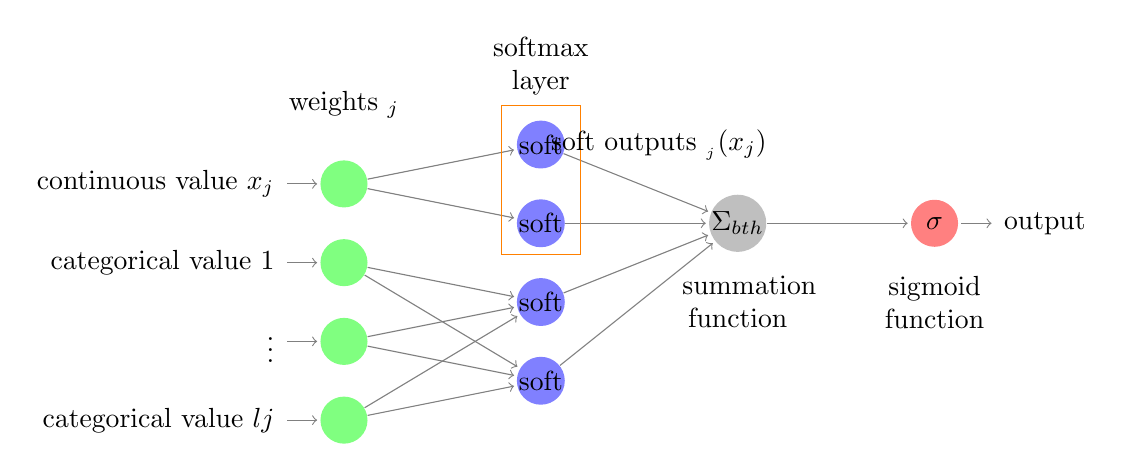
\begin{tikzpicture}[shorten >=1pt,->,draw=black!50, node distance=\layersep]
    \tikzstyle{every pin edge}=[<-,shorten <=1pt]
    \tikzstyle{neuron}=[circle,fill=black!25,minimum size=17pt,inner sep=0pt]
    \tikzstyle{input neuron}=[neuron, fill=green!50];
    \tikzstyle{output neuron}=[neuron, fill=red!50];
    \tikzstyle{hidden neuron}=[neuron, fill=blue!50];
    \tikzstyle{annot} = [text width=4em, text centered]
    \tikzstyle{annotrectangle} = [text width=8em, text centered]


        \node[input neuron, pin=left:continuous value $\gls{x}_j$] (I-1) at (0,-1) {};
        
        \node[input neuron, pin=left:categorical value $1$] (I-2) at (0,-2) {};
        \node[input neuron, pin=left:$\vdots$] (I-3) at (0,-3) {};
        \node[input neuron, pin=left:categorical value $\gls{lj}$] (I-4) at (0,-4) {};

    % Draw the hidden layer nodes
    \foreach \name / \y in {1,...,2}
        \path[yshift=0.5cm]
            node[hidden neuron] (H-\name) at (\layersep,-\y cm) {soft};

    \foreach \name / \y in {3,...,4}
        \path[yshift=0.5cm]
            node[hidden neuron] (H-\name) at (\layersep,-\y cm) {soft};
            
    % Draw the sum layer node 
    
    \node[neuron, right of=H-2] (S) {$\Sigma_{\gls{bth}}$};

    % Draw the output layer node
    
    \node[output neuron,pin={[pin edge={->}]right:output}, right of=S] (O) {$\sigma$};
    
    %\node[output neuron,pin={[pin edge={->}]right:Output}, right of=H-2] (O) {$\sigma(\cdot)$};
    
    

    % Connect every node in the input layer with every node in the
    % hidden layer.
%    \foreach \source in {1,...,4}
        \foreach \dest in {1,2}
            \path (I-1) edge (H-\dest);

        \foreach \dest in {3,4}
            \path (I-2) edge (H-\dest);
        \foreach \dest in {3,4}
            \path (I-3) edge (H-\dest);
        \foreach \dest in {3,4}
            \path (I-4) edge (H-\dest);

        % \foreach \dest in {5,6}
        %     \path (I-3) edge (H-\dest);

    % Connect every node in the hidden layer with the output layer
    \foreach \source in {1,...,4}
        \path (H-\source) edge (S);
        
    % connect Sigma with sigma
    \path (S) edge (O);

    % Annotate the layers
    \node[annot,above of=H-1, node distance=1cm] (hl) {softmax layer};
    \node[annot,above of=I-1,node distance=1cm] {weights $\ag_j$};
    %\node[annot,right of=hl] (s) {};
    \node[annot, below of=O, node distance=1cm] (s) {sigmoid function};
    \node[annot, below of=S,node distance=1cm] {summation function};
    
    \draw [orange] (2,0) rectangle (3,-1.9);
    % \draw [red] (2,-2) rectangle (3,-4);
    
    \node[annotrectangle,right of=H-1, node distance=1.5cm] {soft outputs $\q_{\ag_j}(\gls{x}_j)$}; 

\end{tikzpicture}
\caption{Proposed shallow architecture to maximize (\ref{eq:lqa}).}
\label{fig:nn}
\end{figure}


\paragraph{Stochastic gradient ascent as a quantization provider}

By relying on stochastic gradient ascent, the smoothed likelihood (\ref{eq:lqa}) can be maximized over $\left(\ag, \gls{bth} \right)$. Due to its convergence properties~\cite{bottou2010large}, the results should be close to the maximizers of the original likelihood (\ref{eq:lq}) if the model is well-specified, when there is a true underlying quantization. However, in the misspecified model case, there is no such guarantee. Therefore, to be more conservative, we evaluate at each training epoch $(s)$ the quantization $\hat{\q}^{(s)}$ resulting from the \textit{maximum a posteriori} procedure explicited in Equation~(\ref{eq:ht}), then classically estimate the \gls{lr} parameter \textit{via} maximum likelihood, as done in Equation~(\ref{eq:lq}):
\begin{equation} \label{eq:lr_param_q}
\hat{\gls{bth}}^{(s)} = \argmax_{\gls{bth}} \ell_{\hat{q}^{(s)}}(\gls{bth}; (\gls{bbx},\gls{bby}))
\end{equation}
and the resulting $\mbox{BIC}(\hat{\gls{bth}}^{(s)})$ as in (\ref{eq:BICq}). If $S$ is a given maximum number of iterations of the stochastic gradient ascent algorithm, the quantization retained at the end is then determined by the optimal epoch
\begin{equation} \label{eq:opt_epoch}
s_\star=\argmin_{s\in \{1,\ldots, S\}} \mbox{BIC}(\hat{\gls{bth}}^{(s)}).
\end{equation}
You can think of $S$ as a computational budget: contrary to classical early stopping rules (\textit{e.g.}\ based on validation loss) used in neural network fitting, this network only acts as a stochastic quantization provider for~\eqref{eq:opt_epoch} which will naturally prevent overfitting. We reiterate that, in~\eqref{eq:opt_epoch}, the BIC can be swapped for the user's favourite model choice criterion.

Lots of optimization algorithms for neural networks have been proposed, which all come with their hyperparameters. As, in the general case, $\ell_{\q_{\ag}}(\gls{bth} ; (\gls{bbx},\gls{bby}))$ of Equation~\eqref{eq:lqa} is not guaranteed to be convex, there might be several local maxima, such that all these optimization methods might diverge, converge to a different maximum, or at least converge in very different numbers of epochs, as can be examplified in Animation~\ref{fig:anim_sgd}\footnote{Reproduced from \url{https://github.com/wassname/viz_torch_optim}}. We chose the RMSProp method, which showed good results and is one of the standard methods.

\begin{figure}[!ht]
\begin{animateinline}[poster=first, controls=all, palindrome, autopause, autoresume, width=\textwidth]{3}
\multiframe{300}{i=1+1}{\includegraphics{figures/chapitre4/optimization_methods/viz-\i.png}}%
\end{animateinline}
\caption{\label{fig:anim_sgd} Animation of several optimization methods (the $\star$ denotes the global maximum).}
\end{figure}

 
\paragraph{Choosing an appropriate number of levels}

Concerning now the number of intervals or factor levels $\boldsymbol{m} = (\gls{mj})_1^d$, they have also to be estimated since in practice they are unknown. Looping over all candidates $\boldsymbol{m}$ is intractable. But in practice, by relying on the \textit{maximum a posteriori} procedure developed in Equation~(\ref{eq:ht}), a lot of unseen factor levels might be dropped, \textit{e.g.}\ if $q_{\ag_{j,h}}(\gls{xij}) \ll 1$ for all training observations $\gls{xij}$, the level $h$ ``vanishes'', \textit{i.e.}\ $\hat{q}_{j,h} = 0$. In practice, we recommend to start with a user-chosen $\gls{bm}=\boldsymbol{m}_{\max}$ and we will see in the experiments of Section~\ref{sec:experiments} that the proposed approach is able to explore small values of $\boldsymbol{m}$ and to select a value $\hat{\boldsymbol{m}}$ drastically smaller than $\boldsymbol{m}_{\max}$. This phenomenon, which reduces the computational burden of the quantization task, is also illustrated in Section~\ref{sec:experiments}.

The full algorithm is described in Appendix~\ref{app1:glmdiscNN}.


\section{An \gls{sem} approach} \label{sec:sem}
 
 
In what follows, the quantization $\q(\gls{bx})$ is seen as a latent feature denoted by $\bm{\mathfrak{Q}}$. The same notations can be introduced for this new feature:  $\bqk$ is an observation of $\bm{\mathfrak{Q}}$, $\bqk_j$ will designate the $j^{\text{th}}$ vectorial component of $\bqk$, $\bbqk$ will designate the $n$-sample, and so on. In the following section, we translate earlier assumptions in probabilitics terms. In the subsequent section, we make good use of these assumptions to provide a continuous relaxation of the quantization problem, as was empirically argumented in Section~\ref{subsec:relaxation}. This relaxation is equivalent to the one proposed in Section~\ref{sec:proposal}, although its use differs drastically, as will be emphasized in Section~\ref{subsec:stoch}.

\subsection{Probabilistic assumptions regarding the quantization latent feature}

Firstly, only the well-specified model case is considered, which translates, with this new latent feature, as a probabilistic assumption:
\begin{equation} \label{hyp:true}
\exists \gls{bthstar}, \bqk^\star \text{s.t.\ } Y \sim p_{\gls{bthstar}}(\cdot | \bqk^\star)
\end{equation}
Secondly, the result of the quantization is assumed to be ``self-contained'' w.r.t.\ the predictive information in $\gls{bx}$, \textit{i.e.}\ it is assumed that all available information about $y$ in $\gls{bx}$ has been ``squeezed'' by quantizing the data:
\begin{equation} \label{hyp:squeeze}
\forall \gls{bx},y,\: p(y|\gls{bx},\bqk) = p(y|\bqk)
\end{equation}
Thirdly, the component-wise nature of the quantization can be stated as:
\begin{equation} \label{hyp:component}
\forall \gls{bx},\bqk,\: p(\bqk|\gls{bx}) = \prod_{j=1}^d p(\bqk_j | \gls{x}_j)
\end{equation}



\subsection{Continuous relaxation of the quantization as seen as fuzzy assignment} \label{subsec:fuzzy}

If we consider the deterministic discretization scheme defined in Section~\ref{sec:model_selection}, we have, analogous to Equation~\eqref{eq:qj}:
$$
p(\bqk_j = \gls{ehmj} | \gls{x}_j) = 1 \text{ if } \gls{x}_j \in C_{j,h},
$$
which is a step function. Rewriting $p(y| \gls{bx})$ by integrating over these new latent features,
% and using hypotheses~\ref{hyp:true}, \ref{hyp:squeeze} and \ref{hyp:component} respectively, 
we get:
\begin{align*}
p(y | \gls{bx}) & = p_{\gls{bthstar}}(y | \bqk^\star) & \text{ (using \eqref{hyp:true}) } \\
& = \sum_{\bqk \in \Q} p(y, \bqk | \gls{bx}) \\
& = \sum_{\bqk \in \Q} p(y | \bqk, \gls{bx}) p(\bqk | \gls{bx}) \\
& = \sum_{\bqk \in \Q} p(y | \bqk) p(\bqk | \gls{bx}) & \text{ (using \eqref{hyp:squeeze}) } \\
& = \sum_{\bqk \in \Q} p(y | \bqk) \prod_{j=1}^d p(\bqk_j | \gls{x}_j) & \text{ (using \eqref{hyp:component}) }
\end{align*}
The well-specified model hypothesis~\eqref{hyp:true} yields for all $\gls{x}_j$, $p(\bqk_j^\star | \gls{x}_j) = 1$. Conversely, for $\bqk \in \Q$ such that $\bqk \cancel{\mathcal{R}_{\gls{T}_n}} \bqk^\star$, there exists a feature $j$ and an observation $\gls{xij}$ such that $p(\bqk_j | \gls{x}_j) = 0$. Consequently, the above sum, over all training observations in $\gls{T}_n$, reduces to:
\begin{align*}
p(\gls{bby} | \gls{bbx}) & = \prod_{i=1}^n p(y_i | \gls{bx}_i) \\
 & = \sum_{\bqk \in \Q} \prod_{i=1}^n p(y_i | \bqk_i) \prod_{j=1}^d p(\bqk_{i,j} | \gls{xij}) \\
 & = \prod_{i=1}^n p(y_i | \bqk_i^\star) \prod_{j=1}^d p(\bqk_{i,j}^\star | \gls{xij})
\end{align*}
Thus, we have :
\[ \bqk^\star = \argmax_{\bqk \in \Q} \prod_{i=1}^n p(y_i | \bqk_i ) \prod_{j=1}^d p(\bqk_{i,j} | \gls{xij}). \]
This new formulation of the best quantization is still intractable since it requires to evaluate all quantizations in $\Q$ just like in~\eqref{eq:BICq}, although all terms except $\bqk^\star$ contribute to $0$ in the above $\argmax$. In the misspecfied model-case however, there is no such guarantee but it can still be claimed that the best candidate $\bqk^\star$ in terms of criterion~\eqref{eq:BICq} dominates the sum.

Our goal in the next section is to generate good candidates $\bbqk$ as in Section~\ref{sec:estim}. Among other things detailed later on, models for $p(y | \bqk)$ and $p(\bqk_j | \gls{x}_j)$ shall be proposed. 
A stochastic ``quantization provider'' is designed as in the previous section. Following arguments of the preceding paragraph, its empirical distribution of generated candidates shall be dominated by $\q^\star$,
%If the resulting MCMC is efficient, $\q^\star$ will be the mode of the empirical distribution of generated candidates,
which, as in Section~\ref{sec:proposal} with the neural network approach, can be selected with the BIC criterion~\eqref{eq:BICq}. Using \eqref{hyp:true}, it seems most natural to use a \gls{lr} for $p( y | \bqk_j)$. Following Section~\ref{sec:proposal} and as was empirically argumented in Section~\ref{subsec:relaxation}, the instrumental distribution $p(\bqk_j | \gls{x}_j)$ will take a similar form as $\q_{\ag}$. 

{\bf For a continuous feature}, we resort to a polytomous logistic regression, similar to the softmax function of Equation~\eqref{eq:softmax} without the over-parametrization (one level per feature $j$, say $\gls{mj}$, is considered reference):
\[ p_{\ag_{j,h}}(\bqk_j = \gls{ehmj} | \gls{x}_j) = \begin{cases} \frac{1}{\sum_{h'=1}^{\gls{mj}-1} \exp(\alpha_{j,h'}^0 + \alpha_{j,h'}^1 \gls{x}_j)} \text{ if } h = \gls{mj}, \\ \frac{\alpha_{j,h}^0 + \alpha_{j,h}^1 \gls{x}_j}{\sum_{h'=1}^{\gls{mj}-1} \exp(\alpha_{j,h'}^0 + \alpha_{j,h'}^1 \gls{x}_j)} \text{ otherwise.} \end{cases} \]
{\bf For categorical features}, simple contingency tables are employed:
\[ p_{\ag_{j,h}^o}(\bqk_j = \gls{ehmj} | \gls{x}_j) = \frac{|\bbqk_{j,h}|}{|\{\gls{x}_j=o\}|} \text{ for } 1 \leq o \leq \gls{lj} \]
Similarly, $p_{\ag_j}(\bqk_j | \gls{x}_j)$ are no more step functions but smooth functions as in Figure~\ref{fig:MAP}.

\paragraph{Remark on polytomous logistic regressions}

Since the resulting latent categorical feature can be interpreted as an ordered categorical features (the \textit{maximum a posterior} operation yields contiguous intervals as argued in Section~\ref{subsec:relaxation}), ordinal ``parallel'' \gls{lr}~\cite{o2006logistic} could be used (provided levels $h$ are reordered). This particular model is of the form:
\[ \ln \frac{p(\bqk_{j} = \bm{e}_{h+1}^{\gls{mj}} | \gls{x}_j)}{p(\bqk_{j} = \gls{ehmj} | \gls{x}_j)} = \alpha_{j,h,0} + \alpha_{j} \gls{x}_j, 1 \leq h < \gls{mj}, \]
which restricts the number of parameters since all levels $h$ share the same slope $\alpha_j$. Its advantages lie in the fact that it might lead to sharper door functions quicker, and that it has fewer parameters to estimate, thus reducing \textit{de facto} the estimation variance of each ``soft'' quantization $p_{\ag_j}$. However, it makes it harder for levels to ``vanish'' which would require to iterate over the number of levels per feature $\gls{mj}$ which we wanted to avoid (see Paragraph~\nameref{par:choosing_sem} in the next section). In practice, it yielded similar results to polytomous \gls{lr} such that they remain a parameter of the \textsf{R} package \textit{glmdisc} (see Appendix~\ref{app2}).

\subsection{Stochastic search of the best quantization} \label{subsec:stoch}

We parametrized $p(y|\gls{bx})$ as:
\begin{equation}
p(y | \gls{bx}, \gls{bth}, \ag) = \sum_{\bqk \in \Q} p_{\gls{bth}}(y | \bqk) \prod_{j=1}^d p_{\ag_j}(\bqk_j | \gls{bbx}_j)
\end{equation}
A straightforward way to maximize the likelihood of $p(y | \gls{bx}, \gls{bth}, \ag)$ in $(\gls{bth}, \ag)$ (not to be mistaken with~\eqref{eq:lqa}), as was done in Section~\ref{sec:proposal}, to deduce $\q^\star$ from $\ag$ \textit{via} the $\argmax$ operation (see Section~\ref{subsec:relaxation} and Equation~\eqref{eq:ht}), is to use an \gls{em} algorithm~\cite{dempster1977maximum}.

However, maximizing this likelihood directly is intractable as the Expectation step requires to sum over $\bqk \in \Q$. Classically, the \gls{em} can be replaced by the \acrlong{sem}~\cite{celeux1985sem} algorithm: the expectation (the sum over $\bqk \in \Q$) is approximated by the empirical distribution of draws $\bqk^{(1)}, \dots, \bqk^{(S)}$ from $p_{\gls{bth}}(y | \cdot) \prod_{j=1}^d p_{\ag_j}(\cdot | \gls{x}_j)$.

\subsubsection{\gls{sem} as a quantization provider}

As the parameters $\ag$ of $\q_{\ag}$ were initialized randomly in the neural network approach, the latent features observations $\bbqk^{(0)}$ are initialized randomly. At step $s$, the \gls{sem} algorithm allows us to compute the \gls{mle} ${\gls{bth}}^{(s)}$ (resp. ${\ag}^{(s)}$) of $\gls{bth}$ (resp. $\ag$) given $\bbqk^{(s)}$ by maximizing the following likelihoods (M-steps):
\begin{alignat}{2}
{\gls{bth}}^{(s)} & = \argmax_{\gls{bth}} \ell(\gls{bth}; \bbqk^{(s)}, \gls{bby}) && = \argmax_{\gls{bth}} \sum_{i=1}^n \ln p_{\gls{bth}}(y_i | \bqk^{(s)}_i), \nonumber \\
{\ag_j}^{(s)} & = \argmax_{\ag_j} \ell(\ag_j; \gls{bbx}_j, \bbqk^{(s)}_j) && = \argmax_{\ag_j} \sum_{i=1}^n \ln p_{\ag_j}(\bqk^{(s)}_{i,j} | \gls{xij}) \text{ for } 1 \leq j \leq d. \label{eq:mle_ag}
\end{alignat}

As the \gls{lr} $p_{\gls{bth}}(y | \bqk)$ is multivariate, it is hard to sample simultaneously all latent features. We have to resort to the Gibbs-sampler~\cite{casella1992explaining}: $\bqk_j$ is sampled while holding latent features $\bqk_{-\{j\}}$ fixed (S-step):
\begin{equation} \label{eq:q_draw}
\bqk_j^{(s+1)} \sim p_{\hat{\gls{bth}}^{(s)}}(y | \bqk_{-\{j\}}^{(s)}, \cdot) p_{\hat{\ag}_j^{(s)}}(\cdot | \gls{x}_j)
\end{equation}
This process is repeated for all features $1 \leq j \leq d$.

This \gls{sem} provides parameters ${\ag}^{(1)}, \dots, {\ag}^{(S)}$ which can be used to produce $\hat{\q}^{(1)}, \dots, \hat{\q}^{(S)}$ following the \textit{maximum a posteriori} scheme from Equation~\eqref{eq:ht}, adapated to this new formulation:
\[ \hat{\q}_j^{(s)}(\cdot) = \argmax_{h} p_{\ag_j^{(s)}}(\gls{ehmj} | \cdot ) .\]
The \gls{lr} parameters $\hat{\gls{bth}}^{(s)}$ on quantized data are obtained similarly as in~\eqref{eq:lr_param_q}. The best proposed quantization $\q^\star$ is thus chosen among them \textit{via e.g.}\ the BIC criterion as in Equation~\eqref{eq:opt_epoch}.


\subsubsection{Validity of the approach}

The pseudo-completed sample $(\gls{bbx}, \bbqk^{(s)}, \gls{bby})$ allows to compute $({\gls{bth}}^{(s)},{\ag}^{(s)})$ which do not converge to the \gls{mle} of $p(\gls{bby} | \gls{bbx}, \gls{bth}, \ag)$, for the simple reason that, being random in essence, it does not converge pointwise. From its authors, the \gls{sem} is however expected to be directed by the \gls{em} dynamics~\cite{celeux_sem} and its empirical distribution converges to the target distribution $p(\gls{bby} | \gls{bbx}, \gls{bth}, \ag)$ provided such a distribution exists and is unique. This existence is guaranteed by remarking that for all features $j$, $ p(\bqk_j | \gls{x}_j, \bqk^{(s)}_{-\{j\}} y, \gls{bth}, \ag) \propto p_{\gls{bth}}(y | \bqk^{(s)}_{-\{j\}}, \bqk_j) p_{\ag_j}(\bqk_j | \gls{x}_j) > 0 $ by definition of the \gls{lr} and polytomous logistic regressions or the contingency tables respectively. The uniqueness is not guaranteed since levels can disappear and there is an absorbing state (the empty model): this point is detailed in the next Section.

In its original purpose~\cite{celeux_sem}, the \gls{sem} was employed either to find good starting points for the \gls{em} (\textit{e.g.}\ to avoid local maxima) or to propose an estimator of the \gls{mle} of the target distribution as the mean or the mode of the resulting empirical distribution, eventually after a burn-in phase. As, in our setting, we are not directly interested in the \gls{mle} but only to the best quantization in the sense of Equation~\eqref{eq:BICq}. The best proposed quantization $\q^\star$ is thus chosen among them \textit{via} the BIC criterion as in Equation~\eqref{eq:opt_epoch} as stated in the previous paragraph.

\subsubsection{Choosing an appropriate number of levels} \label{par:choosing_sem}

Contrary to the neural network approach developed in Section~\ref{sec:proposal}, the \gls{sem} algorithm alternates between drawing $\bbqk^{(s)}$ and fitting ${\gls{bth}}^{(s)}$ and ${\ag}^{(s)}$  at each step $s$. Therefore, additionally to the phenomenon of ``vanishing'' levels caused by the \textit{maximum a posteriori} procedure similar to the neural network approach, if a level $h$ of $\bqk$ is not drawn, following Equation~\eqref{eq:q_draw}, at step $s$, then at step $s+1$ when adjusting parameters $\ag_j$ by maximum likelihood from Equation~\eqref{eq:mle_ag}, this level will have disappeared and cannot be drawn again. A Reversible-Jump MCMC approach would be needed~\cite{green1995reversible} to ``resuscitate'' these levels, which is not needed in the neural network approach because its architecture is fixed in advance. As a consequence, with a design matrix of fixed size $n$, there is a non-zero probability that for any given feature, any of its levels collapses at each step such that $\gls{mj}^{(s+1)} \leftarrow \gls{mj}^{(s)} - 1$.

The MCMC has thus an absorbing state for which all features are quantized into one level (the empty model with no features) which is reached in a finite number of steps (although very high if $n$ is sufficiently large as is the case with \textit{Credit Scoring} data). The \gls{sem} algorithm is an effective way to start from a high number of levels per feature $\gls{bm}_{\max}$ and explore smaller values.

The full algorithm is described in Appendix~\ref{app1:glmdiscSEM}.

\section{Numerical experiments} \label{sec:experiments}

This section is divided into three complementary parts to assess the validity of our proposal, that is called hereafter \textit{glmdisc}-NN and \textit{glmdisc}-SEM, designating respectively the approaches developed in Sections~\ref{sec:proposal} and~\ref{sec:sem}. First, simulated data are used to evaluate its ability to recover the true data generating mechanism. Second, the predictive quality of the new learned representation approach is illustrated on several classical benchmark datasets from the UCI library. Third, we use it on \textit{Credit Scoring} datasets provided by \gls{cacf}. The code of all experiments, excluding the confidential real data, can be retrieved following the guidelines in Appendix~\ref{app2}.


\subsection{Simulated data: empirical consistency and robustness}

Focus is here given on discretization of continuous features (similar experiments could be conducted on categorical ones). Two continuous features $\gls{x}_1$ and $\gls{x}_2$ are sampled from the uniform distribution on $[0,1]$ and discretized as exemplified on Figure~\ref{fig:exp_sim} by using
\[\q_1(\cdot)=\q_2(\cdot) = (\mathds{1}_{]-\infty,1/3]}(\cdot),\mathds{1}_{]1/3,2/3]}(\cdot),\mathds{1}_{]2/3,\infty[}(\cdot)).\]
Here, following (\ref{eq:Cjhcont}), we have $d=2$ and $m_1=m_2=3$ and the cutpoints are $c_{j,1}=1/3$ and $c_{j,2}=2/3$ for $j=1,2$. Setting $\gls{bth}=(0,-2,2,0,-2,2,0)$, the target feature $y$ is then sampled from $p_{\gls{bth}}(\cdot | \q(\gls{bbx}))$ via the logistic model (\ref{eq:reglogq}).

\begin{figure}[!ht]
\centering
\begin{tikzpicture}
      \draw[->] (-1,0) -- (9,0) node[right] {$\gls{x}$};
      \draw[->] (0,-1) -- (0,3) node[above] {$p(\gls{x})$};
      \draw[scale=1,domain=0.5:7,smooth,variable=\y,red,thick]  plot ({\y},2.5);
      \draw[scale=1,domain=-1:0.5,smooth,variable=\y,red,thick]  plot ({\y},0);
      \draw[scale=1,domain=7:8.5,smooth,variable=\y,red,thick]  plot ({\y},0);
      \draw[scale=1,domain=0:2.5,smooth,variable=\x,red]  plot (0.5,{\x});
      \draw[scale=1,domain=0:2.5,smooth,variable=\x,red]  plot (7,{\x});
      
      \draw[scale=1,domain=-0.2:2.8,smooth,variable=\x,blue]  plot (2.67,{\x});
      \draw[scale=1,domain=-0.2:2.8,smooth,variable=\x,blue]  plot (4.83,{\x});

		\node[scale=0.7] (q1) at  (1.2,2.7) {\small $\q(\gls{x})=(1,0,0)$};
		\node[scale=0.7] (q2) at  (3.5,2.7) {\small $\q(\gls{x})=(0,1,0)$};
		\node[scale=0.7] (q3) at  (6,2.7) {\small $\q(\gls{x})=(0,0,1)$};

		\node[scale=0.7] (x1) at  (0.5,-0.5) {$0$};
		\node[scale=0.7] (x2) at  (2.67,-0.5) {$c_1=1/3$};
		\node[scale=0.7] (x3) at  (4.83,-0.5) {$c_2=2/3$};
		\node[scale=0.7] (x4) at  (7,-0.5) {$1$};

\end{tikzpicture}
\caption{\label{fig:exp_sim} Pdf of the simulated continuous data $\gls{x}$ and the true quantization $\q$.}
\end{figure}


From the \textit{glmdisc} algorithm, we studied three cases:
\begin{enumerate}[(a)]
    \item First, the quality of the cutoff estimator $\hat{c}_{j,2}$ of $c_{j,2} = 2/3$ is assessed when the starting maximum number of intervals per discretized continuous feature is set to its true value $m_1=m_2= 3$;
    \item Second, I estimated the number of intervals $\hat{m}_1$ of $m_1=3$ when the starting maximum number of intervals per discretized continuous feature is set to $m_{\text{max}} = 10$; 
    \item Last, I added a third feature $\gls{x}_3$ also drawn uniformly on $[0,1]$ but uncorrelated to $\gls{y}$ and estimated the number $\hat{m}_3$ of discretization intervals selected for $\gls{x}_3$. The reason is that a non-predictive feature which is discretized or grouped into a single value is \textit{de facto} excluded from the model, and this is a positive side effect.
\end{enumerate}
From a statistical point of view, experiment (a) assesses the empirical consistency of the estimation of $C_{j,h}$, whereas experiments (b) and (c) focus on the consistency of the estimation of $\gls{mj}$. The results are summarized in Table~\ref{tab:estim_precision} where 95\% confidence intervals (CI~\cite{sun2014fast}) are given, with a varying sample size. Note in particular that the slight underestimation in (b) is a classical consequence of the BIC criterion on small samples. 

\begin{table}[ht]
    \centering
    \caption{For \textit{glmdisc}-NN and \textit{glmdisc}-SEM and different sample sizes $n$, (A) CI of $\hat{c}_{j,2}$ for $c_{j,2} = 2/3$. (B) Bar plot of $\hat{m} = 2, 3, 4$ (resp.) for $m_1=3$. (C) Bar plot of $\hat{m}_3 = 1, 2, 3$ (resp.) for $m_3=1$.}
    \label{tab:estim_precision}
\begin{tabular}{lllllll}
Algorithm & $n$ & (a) $\hat{c}_{j,2}$ & (b) & $\hat{m}_1$ & (c) & $\hat{m}_3$ \\
\hline
\hline
\textit{glmdisc}-NN & $1{,}000$ & $[0.656,0.666]$ & \myobar{9}{90}{1} & \mybar{60}{32}{8} \\
\textit{glmdisc}-SEM & $1{,}000$ & $[0.664,0.669]$ & \myobar{2}{53}{44} & \mybar{34}{56}{10} \\
\hline
\textit{glmdisc}-NN & $10{,}000$ & $[0.666,0.666]$ & \myobar{0}{100}{0} & \mybar{88}{12}{0} \\
\textit{glmdisc}-SEM & $10{,}000$ & $[0.666,0.666]$ & \myobar{2}{69}{30} & \mybar{30}{48}{22}
\end{tabular}
\end{table}

To complement these experiments on simulated data following a well-specified model, a similar study can be done for categorical features: 10 levels are drawn uniformly and 3 groups of levels, which share the same log-odd ratio, are created. The same phenomenon as in Table~\ref{tab:estim_precision} is witnessed: the empirical distribution of the estimated number of groups of levels is peaked at its true value of 3.

Finally, it was argued in Section~\ref{sec:model_selection} that by considering all features when quantizing the data, relying on a multivariate approach could yield better results than classical univariate techniques in presence of correlation. This claim is verified in Table~\ref{tab:sim_false} where multivariate heteroskedastic gaussian data is simulated on which the log odd ratio of $y$ depends linearly (misspecified model setting for the quantized \gls{lr}). The proposed approach yields significantly better results.

\begin{table}[ht]
    \centering
    \caption{Gini of the resulting misspecified \gls{lr} from quantized data using ChiMerge, MDLP and \textit{glmdisc}-SEM: the multivariate approach is able to capture information about the correlation structure.}
    \label{tab:sim_false}
\begin{tabular}{llll}
 & ChiMerge & MDLP & \textit{glmdisc}-SEM \\
\hline
Performance & 50.1 (1.6) & 77.1 (0.9) & \textbf{80.6} (0.6)
\end{tabular}
\end{table}



 \newlength\figureheight
 \newlength\figurewidth
 \setlength\figureheight{4cm}
 \setlength\figurewidth{14cm}
 
  \begin{figure}[!ht]
    \centering
    \begin{subfigure}[t]{\textwidth}
        \centering
        % This file was created by matplotlib2tikz v0.6.18.
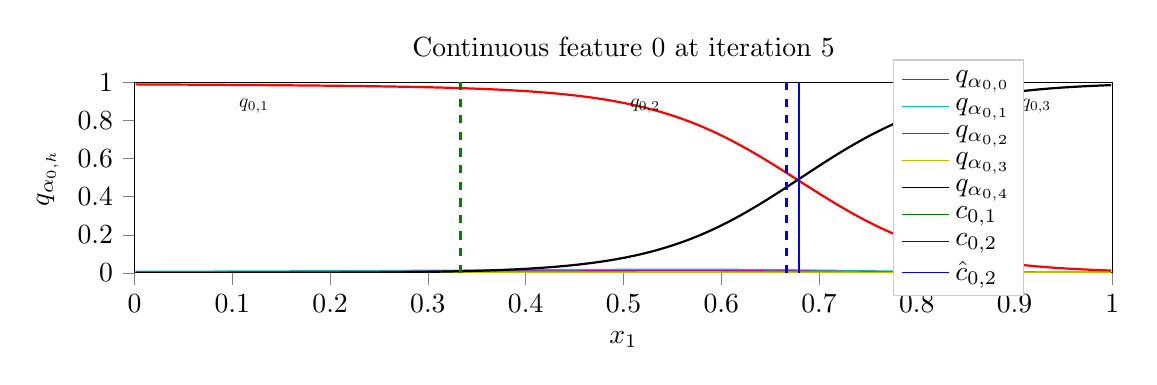
\begin{tikzpicture}

\definecolor{color0}{rgb}{0,0.75,0.75}
\definecolor{color1}{rgb}{0.75,0,0.75}
\definecolor{color2}{rgb}{0.75,0.75,0}

\begin{axis}[
height=\figureheight,
legend cell align={left},
legend entries={{${q}_{\bm{\alpha}_{0,0}}$},{${q}_{\bm{\alpha}_{0,1}}$},{${q}_{\bm{\alpha}_{0,2}}$},{${q}_{\bm{\alpha}_{0,3}}$},{${q}_{\bm{\alpha}_{0,4}}$},{$c_{0,1}$},{$c_{0,2}$},{$\hat{c}_{0,2}$}},
legend style={at={(0.91,0.5)}, anchor=east, draw=white!80.0!black},
tick align=outside,
tick pos=left,
title={Continuous feature 0 at iteration 5},
width=\figurewidth,
x grid style={white!69.01960784313725!black},
xlabel={$x_1$},
xmin=0, xmax=1,
y grid style={white!69.01960784313725!black},
ylabel={${q}_{\bm{\alpha}_{0,h}}$},
ymin=0, ymax=1
]
\addlegendimage{no markers, red}
\addlegendimage{no markers, color0}
\addlegendimage{no markers, color1}
\addlegendimage{no markers, color2}
\addlegendimage{no markers, black}
\addlegendimage{no markers, green!50.0!black}
\addlegendimage{no markers, blue}
\addlegendimage{no markers, blue}
\addplot [thick, red]
table [row sep=\\]{%
0.0011059794751318	0.990096211433411 \\
0.00144600828615515	0.990088164806366 \\
0.00151620394328711	0.990086495876312 \\
0.00161381928831428	0.990084171295166 \\
0.00193644961641948	0.99007648229599 \\
0.0024363370221504	0.990064680576324 \\
0.00384167794354173	0.990030884742737 \\
0.00421063900202368	0.990022242069244 \\
0.00632372037002726	0.989971518516541 \\
0.00947686783375368	0.989895045757294 \\
0.0099356428556221	0.989883720874786 \\
0.0101317191976503	0.989879012107849 \\
0.0102519961026396	0.989876091480255 \\
0.0116572936797861	0.989841759204865 \\
0.0122763055741271	0.989826560020447 \\
0.0128807282915644	0.989811718463898 \\
0.0131006826676461	0.989806354045868 \\
0.0132105085232722	0.989803791046143 \\
0.0150477352877949	0.989758253097534 \\
0.0151511241047927	0.989755690097809 \\
0.0168553495563415	0.989713549613953 \\
0.0191895991753259	0.989655137062073 \\
0.0192724193499449	0.989653170108795 \\
0.0202131188025382	0.989629566669464 \\
0.0251886934986562	0.989503502845764 \\
0.0255409812646521	0.989494621753693 \\
0.0256196546755231	0.989492535591125 \\
0.0263800727822662	0.989473164081573 \\
0.026825697968402	0.989461719989777 \\
0.0272388337061176	0.989451229572296 \\
0.0276781997826389	0.989439904689789 \\
0.0277969734855988	0.989436745643616 \\
0.027888291941232	0.98943430185318 \\
0.032801074197002	0.989307105541229 \\
0.0337126623182875	0.989283204078674 \\
0.0349109578825388	0.989251792430878 \\
0.0367757145561887	0.989202558994293 \\
0.0368887253476963	0.989199638366699 \\
0.0376301111814882	0.989180088043213 \\
0.0383020767002249	0.989162087440491 \\
0.0385765124363792	0.989154756069183 \\
0.0386281055032889	0.989153444766998 \\
0.0397134557815922	0.989124536514282 \\
0.0400530872540832	0.989115476608276 \\
0.0408224228009035	0.989094793796539 \\
0.042416614098386	0.989051878452301 \\
0.042542997860721	0.989048600196838 \\
0.0425634328976269	0.989048182964325 \\
0.0426938593122377	0.989044547080994 \\
0.0436353215690566	0.989019095897675 \\
0.0476491609572692	0.988909900188446 \\
0.0476764809468383	0.988909184932709 \\
0.0480632979275277	0.988898575305939 \\
0.0489335324060199	0.988874673843384 \\
0.0494953541501341	0.988859176635742 \\
0.0498656975684827	0.988848924636841 \\
0.0507299142819697	0.988825023174286 \\
0.0520149216066462	0.988789319992065 \\
0.053491737186121	0.98874819278717 \\
0.0545456118282759	0.988718867301941 \\
0.0549368100196436	0.988707900047302 \\
0.0549667939602374	0.988706946372986 \\
0.0555159955251522	0.988691568374634 \\
0.0574839546417889	0.988636016845703 \\
0.0576927502423773	0.988630056381226 \\
0.0580609228746025	0.988619565963745 \\
0.0610070220733733	0.988535583019257 \\
0.0613718310828713	0.988525211811066 \\
0.0624819644863142	0.988493263721466 \\
0.0632024977130776	0.988472521305084 \\
0.0641707318537266	0.988444447517395 \\
0.064803290117067	0.988426208496094 \\
0.0661546388560771	0.988386809825897 \\
0.0675945492445934	0.988344788551331 \\
0.0701208744758773	0.988270401954651 \\
0.0704495440664726	0.988260746002197 \\
0.0707913481046274	0.988250613212585 \\
0.0709503961374458	0.988245725631714 \\
0.0723079949898875	0.988205313682556 \\
0.0729582139062805	0.988186001777649 \\
0.0736427592129116	0.988165497779846 \\
0.0738431652021745	0.988159537315369 \\
0.074094042941424	0.988152086734772 \\
0.0741988699821797	0.988148748874664 \\
0.0745344402647278	0.988138735294342 \\
0.0761651718345726	0.988089501857758 \\
0.0762565104011357	0.988086819648743 \\
0.0764247618188199	0.988081812858582 \\
0.0780473992355428	0.988032579421997 \\
0.0784939963588281	0.988018870353699 \\
0.0787288834363844	0.988011837005615 \\
0.0796528614743472	0.987983345985413 \\
0.0821291956626848	0.987907350063324 \\
0.0836539892117674	0.987860023975372 \\
0.0837976822096664	0.987855732440948 \\
0.0840863722935196	0.987846791744232 \\
0.0847664004367794	0.987825334072113 \\
0.0848642352310873	0.987822473049164 \\
0.0852150851090396	0.987811505794525 \\
0.085891869345856	0.98779034614563 \\
0.087068315817913	0.987753331661224 \\
0.0885849846877879	0.98770546913147 \\
0.0903431131516136	0.987649619579315 \\
0.0909278592293694	0.987630903720856 \\
0.0914296081009306	0.987614989280701 \\
0.0922298300096035	0.987589418888092 \\
0.0926517333242025	0.987575769424438 \\
0.0930086769471365	0.987564265727997 \\
0.0936368650628759	0.987544059753418 \\
0.0939832817677504	0.987532913684845 \\
0.0963578674192209	0.987455725669861 \\
0.0969604240071604	0.987436056137085 \\
0.0974174263218397	0.987421154975891 \\
0.0997464409700664	0.98734450340271 \\
0.100249930959155	0.987327754497528 \\
0.100820744388044	0.987308919429779 \\
0.101229398304142	0.98729532957077 \\
0.102271393895604	0.987260580062866 \\
0.102325882258744	0.987258732318878 \\
0.103474916599901	0.987220406532288 \\
0.104369461810087	0.987190425395966 \\
0.104849386693897	0.987174034118652 \\
0.105274572558957	0.987159729003906 \\
0.105437385176067	0.987154245376587 \\
0.105718642159513	0.987144768238068 \\
0.106451679001465	0.987119913101196 \\
0.106754108203929	0.987109661102295 \\
0.106889477031479	0.987105011940002 \\
0.108308586301563	0.987056612968445 \\
0.108355506097126	0.987054944038391 \\
0.110864090628752	0.986968576908112 \\
0.112062699234041	0.986927092075348 \\
0.112686863552251	0.986905515193939 \\
0.113787419472266	0.986867070198059 \\
0.114114908535732	0.986855447292328 \\
0.114926076298882	0.98682701587677 \\
0.115710925433917	0.986799418926239 \\
0.116193807044869	0.986782312393188 \\
0.116352662276253	0.986776649951935 \\
0.116979956596317	0.986754596233368 \\
0.117247317403657	0.986745059490204 \\
0.118793828877862	0.986689925193787 \\
0.119352906137166	0.986669838428497 \\
0.120388240876593	0.986632704734802 \\
0.122357154089364	0.986561357975006 \\
0.125712799722249	0.986438751220703 \\
0.126988316690772	0.986391663551331 \\
0.130289689058528	0.986268401145935 \\
0.130830575131366	0.986247956752777 \\
0.13178708265069	0.986211776733398 \\
0.132217070962463	0.98619544506073 \\
0.132641072460891	0.986179351806641 \\
0.133694684584262	0.986139118671417 \\
0.135586813424106	0.986066520214081 \\
0.136970534315695	0.986012995243073 \\
0.137167897059254	0.986005425453186 \\
0.13731957841644	0.985999643802643 \\
0.138770949832641	0.985942959785461 \\
0.141579671494468	0.985832333564758 \\
0.142337772861435	0.985802233219147 \\
0.142852169410084	0.985781610012054 \\
0.14313843453823	0.985770225524902 \\
0.143709892765619	0.985747277736664 \\
0.143996587198751	0.985735833644867 \\
0.144338718134467	0.985722303390503 \\
0.145474509131844	0.985676288604736 \\
0.146058924442183	0.985652804374695 \\
0.147496370200373	0.98559433221817 \\
0.147934500473159	0.985576450824738 \\
0.148464696403164	0.985554695129395 \\
0.149007159183894	0.985532462596893 \\
0.151290695331351	0.985438108444214 \\
0.153507740604538	0.985345423221588 \\
0.153927498261582	0.98532772064209 \\
0.153953160827713	0.985326647758484 \\
0.154179436777791	0.985317170619965 \\
0.155107736993068	0.985277831554413 \\
0.15519005879533	0.985274434089661 \\
0.155418402417591	0.985264718532562 \\
0.156078407887877	0.985236644744873 \\
0.158100170599977	0.98514997959137 \\
0.158283533549941	0.985142171382904 \\
0.158599777942073	0.98512852191925 \\
0.159258263288539	0.985100209712982 \\
0.159678910282026	0.985081911087036 \\
0.162540881855109	0.984956681728363 \\
0.164077384668961	0.984888792037964 \\
0.164957348092599	0.984849691390991 \\
0.165030574098427	0.984846472740173 \\
0.165280388241905	0.984835386276245 \\
0.167273692684132	0.984745621681213 \\
0.168043854724866	0.984710872173309 \\
0.168088628486329	0.984708905220032 \\
0.168662857989897	0.984682738780975 \\
0.169151147716595	0.984660446643829 \\
0.169673214248392	0.984636664390564 \\
0.170135609058708	0.984615385532379 \\
0.171767974673073	0.984540283679962 \\
0.1728518498484	0.984490036964417 \\
0.172984599941167	0.984483897686005 \\
0.176370551959836	0.98432457447052 \\
0.176588273575192	0.984314322471619 \\
0.176656553576852	0.984311044216156 \\
0.17794804219768	0.984249413013458 \\
0.178429717033185	0.984226286411285 \\
0.179458814233081	0.984176635742188 \\
0.180595104426831	0.984121680259705 \\
0.18064479669491	0.984119236469269 \\
0.182294707450728	0.984038591384888 \\
0.182819109355123	0.984012842178345 \\
0.189141614514094	0.983695864677429 \\
0.190723527970293	0.983614504337311 \\
0.192508826701743	0.983521819114685 \\
0.200712508340217	0.983083128929138 \\
0.202130410523186	0.983005046844482 \\
0.202705868873484	0.982973217964172 \\
0.202975660615516	0.982958137989044 \\
0.2033001668374	0.982939958572388 \\
0.204138047670012	0.982893168926239 \\
0.204584283026216	0.982868194580078 \\
0.205975712225296	0.982789635658264 \\
0.208693969096644	0.982634127140045 \\
0.209097012308874	0.982610762119293 \\
0.210129299396579	0.982550919055939 \\
0.210470524326312	0.982531011104584 \\
0.210726758187617	0.982516050338745 \\
0.210879765452585	0.982507050037384 \\
0.213404555935633	0.982357859611511 \\
0.214779680955682	0.982275724411011 \\
0.215976334819965	0.982203483581543 \\
0.21605980843853	0.982198417186737 \\
0.21626681121775	0.982185900211334 \\
0.217333435243771	0.982120931148529 \\
0.217860184045886	0.982088625431061 \\
0.218810300034316	0.982030212879181 \\
0.219036830922259	0.982016265392303 \\
0.219186045259484	0.982006967067719 \\
0.219509161852637	0.981986999511719 \\
0.219517283100912	0.981986403465271 \\
0.220007941128277	0.981955945491791 \\
0.221124031401732	0.981886148452759 \\
0.221655686766872	0.981852829456329 \\
0.222787328400317	0.981781363487244 \\
0.222812240344664	0.981779634952545 \\
0.224413114839207	0.98167759180069 \\
0.225712117798195	0.98159384727478 \\
0.226064824403414	0.981570899486542 \\
0.22778297811216	0.981458723545074 \\
0.227786137279108	0.981458604335785 \\
0.228255816092263	0.981427669525146 \\
0.22886379454373	0.981387257575989 \\
0.229286896531361	0.981359362602234 \\
0.231570483736477	0.981206357479095 \\
0.232839821990075	0.98112028837204 \\
0.234699792231533	0.98099285364151 \\
0.236598748956898	0.980860710144043 \\
0.236914864918852	0.980838418006897 \\
0.238193170258512	0.980748295783997 \\
0.238267801131912	0.980743169784546 \\
0.241280255564163	0.98052704334259 \\
0.241532477911657	0.980508804321289 \\
0.242724887440966	0.980421721935272 \\
0.243487528482621	0.980365574359894 \\
0.243851755033328	0.980338871479034 \\
0.243931127736832	0.980332911014557 \\
0.245492487219521	0.980216801166534 \\
0.245961870318215	0.980181634426117 \\
0.247220233087027	0.980086445808411 \\
0.248029547774932	0.980025112628937 \\
0.248195183805212	0.980012357234955 \\
0.252597476547261	0.97967004776001 \\
0.254049623190913	0.97955459356308 \\
0.254469169693275	0.979520857334137 \\
0.254777550536903	0.9794961810112 \\
0.254877558399671	0.9794881939888 \\
0.257253649731868	0.979295134544373 \\
0.257671137054733	0.979260742664337 \\
0.26187840669548	0.978908538818359 \\
0.264182169008257	0.978710412979126 \\
0.265462287195374	0.978598713874817 \\
0.267638564660905	0.978406071662903 \\
0.268216851612881	0.978354394435883 \\
0.269980014659659	0.978195011615753 \\
0.270837940398052	0.978116631507874 \\
0.271133018969332	0.97808963060379 \\
0.271522794293612	0.978053689002991 \\
0.272730212426688	0.977941691875458 \\
0.27325151773824	0.977893173694611 \\
0.273458501731612	0.977873682975769 \\
0.275787496734588	0.977653026580811 \\
0.275790346826632	0.977652788162231 \\
0.275963502468307	0.977636277675629 \\
0.276441724078765	0.977590441703796 \\
0.277788622824976	0.977460145950317 \\
0.278249554181787	0.977415263652802 \\
0.278902433397602	0.977351307868958 \\
0.280228184178203	0.977220237255096 \\
0.282170737525181	0.977025628089905 \\
0.284775883532131	0.976759314537048 \\
0.285319633849948	0.976702868938446 \\
0.285945143849347	0.976637721061707 \\
0.287293498153222	0.976496040821075 \\
0.288098109983407	0.976410686969757 \\
0.288474372887691	0.976370573043823 \\
0.288733693686359	0.976342856884003 \\
0.291563977198166	0.97603577375412 \\
0.293976605993451	0.975768089294434 \\
0.294014528290392	0.97576367855072 \\
0.294718175832172	0.975684463977814 \\
0.294831463459233	0.975671648979187 \\
0.294887681144015	0.975665271282196 \\
0.299064488228799	0.975183427333832 \\
0.299223468133874	0.975164771080017 \\
0.299853491506122	0.975090265274048 \\
0.301624334890634	0.974878787994385 \\
0.302100714632492	0.974821269512177 \\
0.302855829384862	0.974729657173157 \\
0.303468685820656	0.974654912948608 \\
0.304335545384868	0.97454822063446 \\
0.305081848845274	0.974455714225769 \\
0.305263786725066	0.974433064460754 \\
0.305511643802704	0.974402070045471 \\
0.30635774546767	0.974296033382416 \\
0.307937429467832	0.974095642566681 \\
0.308578187230734	0.974013686180115 \\
0.313991998160918	0.973299562931061 \\
0.315973848719028	0.973028957843781 \\
0.317413649622303	0.97282874584198 \\
0.319657848506035	0.972511410713196 \\
0.319781920771261	0.972493708133698 \\
0.320496004308145	0.972391188144684 \\
0.320601310305949	0.972375869750977 \\
0.322246867517597	0.972136557102203 \\
0.323306124649751	0.971980512142181 \\
0.323664358184811	0.971927285194397 \\
0.323805398711091	0.971906304359436 \\
0.324816846999054	0.971755027770996 \\
0.325263683488062	0.97168755531311 \\
0.327533460856979	0.971340835094452 \\
0.328385869951453	0.971208572387695 \\
0.329844054701458	0.970979809761047 \\
0.33074904970515	0.970836043357849 \\
0.332974695502457	0.970476984977722 \\
0.333600133199531	0.970374703407288 \\
0.336001356191777	0.969975829124451 \\
0.338057278352338	0.969626247882843 \\
0.33940563378102	0.969393193721771 \\
0.339522610836627	0.969372808933258 \\
0.341295751839904	0.969060778617859 \\
0.343025583329651	0.968751013278961 \\
0.344156227439929	0.968545436859131 \\
0.344485478041551	0.968485295772552 \\
0.346631556569637	0.968087196350098 \\
0.348247004908186	0.967781722545624 \\
0.348257869791207	0.967779576778412 \\
0.350134953366802	0.96741795539856 \\
0.352271571140202	0.966997742652893 \\
0.352403536611892	0.966971576213837 \\
0.356607161458692	0.966115713119507 \\
0.357473355861859	0.965934634208679 \\
0.359032837138255	0.965604305267334 \\
0.360085447455855	0.965378224849701 \\
0.360587038984981	0.965269505977631 \\
0.3618814720936	0.964986562728882 \\
0.362541325151431	0.964840710163116 \\
0.363971114014582	0.964521467685699 \\
0.36446377318254	0.964410364627838 \\
0.364734654416428	0.964348793029785 \\
0.364782079325344	0.964338064193726 \\
0.36626622804169	0.96399849653244 \\
0.36745676602671	0.963722169399261 \\
0.367555756327517	0.963698923587799 \\
0.367766921022286	0.963649451732635 \\
0.368015883464081	0.9635910987854 \\
0.368183587302196	0.963551580905914 \\
0.368646745255496	0.963442385196686 \\
0.368824340831231	0.96340024471283 \\
0.36908666014638	0.963337957859039 \\
0.370227788452905	0.963064968585968 \\
0.371079364739364	0.962859034538269 \\
0.371457393668236	0.962767004966736 \\
0.372521553247257	0.96250593662262 \\
0.372816229090882	0.962433159351349 \\
0.373696444358129	0.962214291095734 \\
0.375236418301489	0.961826264858246 \\
0.375355278624935	0.961796045303345 \\
0.375592850161798	0.961735367774963 \\
0.375621310337888	0.961728096008301 \\
0.37623340048021	0.961571455001831 \\
0.376649481158299	0.961464464664459 \\
0.37682934901581	0.96141791343689 \\
0.377022374188538	0.961368024349213 \\
0.378777395062222	0.960908889770508 \\
0.379219181502585	0.960792005062103 \\
0.380639994297166	0.960412204265594 \\
0.381635433931239	0.960142314434052 \\
0.382416367624347	0.959928631782532 \\
0.383276747323035	0.959691107273102 \\
0.383441774868681	0.959645390510559 \\
0.384589480637987	0.959324300289154 \\
0.38762147240542	0.958456873893738 \\
0.387652450706726	0.958447873592377 \\
0.38818745089578	0.95829164981842 \\
0.388531576179462	0.958190679550171 \\
0.391108514236782	0.957422435283661 \\
0.391741157295481	0.957230687141418 \\
0.396723908263121	0.955670952796936 \\
0.39803082540264	0.955247402191162 \\
0.398171926406937	0.955201148986816 \\
0.398666017137866	0.955039083957672 \\
0.398819673578751	0.954988658428192 \\
0.4012576168302	0.954174697399139 \\
0.402752737045505	0.953664541244507 \\
0.403290070599278	0.953479111194611 \\
0.404563584871068	0.953034937381744 \\
0.406532702382757	0.952336013317108 \\
0.406578018270242	0.95231956243515 \\
0.413273296435021	0.949822723865509 \\
0.413592377461711	0.949698925018311 \\
0.41401191876112	0.949535548686981 \\
0.414776267969876	0.949235856533051 \\
0.414785799829368	0.94923210144043 \\
0.415238430177184	0.949053406715393 \\
0.416465974154779	0.948564112186432 \\
0.416689013292801	0.948474586009979 \\
0.418297500020148	0.947821736335754 \\
0.422720878338663	0.945963680744171 \\
0.424343600824592	0.945258438587189 \\
0.425257001696199	0.944855868816376 \\
0.42710227803989	0.944029569625854 \\
0.427962517509508	0.943638324737549 \\
0.429309169026115	0.943018615245819 \\
0.429443446115563	0.942956387996674 \\
0.429705476003957	0.942834436893463 \\
0.431003390699289	0.942225277423859 \\
0.432539042653788	0.941492736339569 \\
0.433068569337496	0.941237270832062 \\
0.433545956268458	0.941005527973175 \\
0.433750136573834	0.94090610742569 \\
0.433778478107147	0.940892279148102 \\
0.434834104829426	0.940374195575714 \\
0.435898870411909	0.939845383167267 \\
0.43750740037395	0.939034342765808 \\
0.437737100851006	0.938917279243469 \\
0.439197385289126	0.93816602230072 \\
0.440921894924801	0.937262892723083 \\
0.442219378180834	0.936571538448334 \\
0.446052885401706	0.934469044208527 \\
0.447759455363191	0.933503150939941 \\
0.448771556188603	0.932921826839447 \\
0.448918332177756	0.932836830615997 \\
0.449861491210787	0.932287991046906 \\
0.449976789412666	0.93222051858902 \\
0.450129821782654	0.932130753993988 \\
0.453058505166632	0.930383682250977 \\
0.455515296612047	0.928872764110565 \\
0.461612686527044	0.924937844276428 \\
0.462183229417738	0.924555659294128 \\
0.46315332653893	0.923900187015533 \\
0.463567773958142	0.923618018627167 \\
0.464569005654222	0.922930955886841 \\
0.46546966357775	0.922306180000305 \\
0.465627783083443	0.922195732593536 \\
0.466166033904132	0.921818792819977 \\
0.466888847202291	0.921308994293213 \\
0.468332203161028	0.920278251171112 \\
0.469094139229819	0.919727563858032 \\
0.469464236056835	0.919458329677582 \\
0.469806075154756	0.919208645820618 \\
0.470776441432414	0.918494880199432 \\
0.471475988022769	0.917975306510925 \\
0.473199954060133	0.916677832603455 \\
0.474832247453521	0.915426313877106 \\
0.475230428162318	0.91511744260788 \\
0.476638306671274	0.914014756679535 \\
0.478988899075304	0.912134945392609 \\
0.479018256118887	0.912111043930054 \\
0.479279919995254	0.911898910999298 \\
0.479532435695615	0.911693453788757 \\
0.479763011578347	0.911505103111267 \\
0.480041882522935	0.911276876926422 \\
0.480923824850651	0.910550653934479 \\
0.481629462985493	0.909964323043823 \\
0.481771508198592	0.90984570980072 \\
0.482503736852496	0.909231722354889 \\
0.483064995688331	0.908757507801056 \\
0.48384062770339	0.908097505569458 \\
0.484085120492796	0.907888293266296 \\
0.484352733912412	0.907658696174622 \\
0.484550939846654	0.907488167285919 \\
0.485022749278845	0.907080709934235 \\
0.485322068953861	0.906821250915527 \\
0.48610300375999	0.906139969825745 \\
0.486253849387163	0.906007766723633 \\
0.489154935058063	0.903421461582184 \\
0.489792628987292	0.902841866016388 \\
0.490458183784177	0.902232706546783 \\
0.492282643359321	0.900540173053741 \\
0.493928358105999	0.898984253406525 \\
0.495701335790147	0.897277057170868 \\
0.496106252426634	0.896882474422455 \\
0.496164487189195	0.89682549238205 \\
0.498739819509518	0.894274115562439 \\
0.500164108812496	0.892832458019257 \\
0.500739446514191	0.89224374294281 \\
0.500830786926564	0.892149984836578 \\
0.502541719930356	0.890376448631287 \\
0.503498564874392	0.889370381832123 \\
0.504534081188611	0.888270020484924 \\
0.504637823699037	0.888159155845642 \\
0.506860898199194	0.885753095149994 \\
0.507491092240963	0.885060489177704 \\
0.508120202534381	0.88436484336853 \\
0.510856303638406	0.881284594535828 \\
0.512327455201249	0.879591703414917 \\
0.51318641739938	0.878591060638428 \\
0.513457954653542	0.878272831439972 \\
0.515863112336536	0.875415325164795 \\
0.516616766484905	0.87450510263443 \\
0.517831355926389	0.873023450374603 \\
0.518931921097757	0.871664762496948 \\
0.521152065672689	0.868876934051514 \\
0.524519468497769	0.864526629447937 \\
0.524576690058109	0.86445140838623 \\
0.525883589956303	0.862721800804138 \\
0.526973717032038	0.861261427402496 \\
0.528680408273136	0.858943045139313 \\
0.530600365407266	0.856287717819214 \\
0.530809662396022	0.855995059013367 \\
0.53166475254574	0.854793667793274 \\
0.532158485575632	0.85409539937973 \\
0.535204926183725	0.849710404872894 \\
0.535356594523575	0.84948867559433 \\
0.537004451507049	0.847058653831482 \\
0.537089668720381	0.846931874752045 \\
0.537190935482585	0.846781194210052 \\
0.538117362047647	0.845395267009735 \\
0.538453506118723	0.844889163970947 \\
0.539359907716354	0.843516826629639 \\
0.539560791003075	0.84321129322052 \\
0.541180326502456	0.840724527835846 \\
0.547271589683928	0.83102285861969 \\
0.548822201570025	0.828463673591614 \\
0.549624872437239	0.8271244764328 \\
0.549819206435189	0.826798737049103 \\
0.550184928091146	0.826184332370758 \\
0.552139674398207	0.822864472866058 \\
0.552982438656419	0.821414768695831 \\
0.5537594353206	0.820068418979645 \\
0.553976139314498	0.819691359996796 \\
0.554051563436848	0.819559931755066 \\
0.55426017856816	0.819195747375488 \\
0.555396555661942	0.817200899124146 \\
0.555501425327998	0.817015826702118 \\
0.556360039382527	0.815493404865265 \\
0.557883446271028	0.812763690948486 \\
0.558670348456701	0.811339199542999 \\
0.559194391744592	0.81038510799408 \\
0.559473603788983	0.809875071048737 \\
0.560198442614008	0.808544635772705 \\
0.560853933269278	0.80733448266983 \\
0.561152915237902	0.806780099868774 \\
0.561401591015197	0.806317985057831 \\
0.562479951006079	0.804302573204041 \\
0.563005908106818	0.803312599658966 \\
0.563050000205171	0.803229629993439 \\
0.563426857102662	0.802517175674438 \\
0.563560604448239	0.802263855934143 \\
0.564062038149409	0.801311492919922 \\
0.565336310962797	0.798872768878937 \\
0.565855772748177	0.797870874404907 \\
0.566858287901599	0.795925199985504 \\
0.566881879040954	0.795879185199738 \\
0.568231608554438	0.793233156204224 \\
0.569223717564581	0.791268885135651 \\
0.569387586449175	0.790942788124084 \\
0.569573989003313	0.790571570396423 \\
0.569720721150053	0.790278792381287 \\
0.572004618116245	0.785676896572113 \\
0.572005154945678	0.785675764083862 \\
0.572151528516064	0.78537791967392 \\
0.57219889974288	0.785281360149384 \\
0.572780347928331	0.784094095230103 \\
0.573600339080632	0.782410204410553 \\
0.576593284261927	0.776169419288635 \\
0.576676798911885	0.775993168354034 \\
0.576819659872325	0.775691270828247 \\
0.577653861143233	0.773922085762024 \\
0.577917937736817	0.773359715938568 \\
0.57793430586259	0.773324608802795 \\
0.581759386894494	0.765045762062073 \\
0.582475032298807	0.763469696044922 \\
0.582896249817215	0.762538135051727 \\
0.589571735768374	0.747377812862396 \\
0.592388904473667	0.740757286548615 \\
0.593611787705259	0.737842679023743 \\
0.594151694891475	0.736547887325287 \\
0.595008948927732	0.734482228755951 \\
0.596105779635777	0.731821835041046 \\
0.597490139381406	0.728435873985291 \\
0.598951438337811	0.724827587604523 \\
0.599201054717089	0.724207758903503 \\
0.600228747033593	0.721645355224609 \\
0.600693928524281	0.720479786396027 \\
0.601589358474053	0.718226373195648 \\
0.602529748251813	0.715845942497253 \\
0.602916831603936	0.714862167835236 \\
0.603866403426713	0.712438344955444 \\
0.606129689323002	0.706603169441223 \\
0.607808363354841	0.702223360538483 \\
0.60811641039762	0.701415002346039 \\
0.608424173673929	0.700605571269989 \\
0.610203299896366	0.695898711681366 \\
0.61052401101773	0.695045053958893 \\
0.611007548691541	0.693754911422729 \\
0.61345268097321	0.687177002429962 \\
0.614300601551049	0.684874773025513 \\
0.616415105925723	0.679087281227112 \\
0.617595625529809	0.675827443599701 \\
0.619695383178102	0.669979572296143 \\
0.620626131680421	0.667367160320282 \\
0.620884093030541	0.666640996932983 \\
0.622959094549987	0.660766005516052 \\
0.624820249131202	0.655446112155914 \\
0.627396892203872	0.648004114627838 \\
0.629679734717881	0.641338348388672 \\
0.63108091324942	0.637214243412018 \\
0.631412061821856	0.636235952377319 \\
0.632209138475077	0.633875846862793 \\
0.632608841524959	0.632689476013184 \\
0.635174872896091	0.625027120113373 \\
0.63680487509045	0.620120048522949 \\
0.638872902814914	0.613851308822632 \\
0.639214862746441	0.61281031370163 \\
0.640549343973947	0.608735322952271 \\
0.6407383188268	0.608156979084015 \\
0.642765742598199	0.601926982402802 \\
0.642772962045468	0.6019047498703 \\
0.644393148200581	0.596896350383759 \\
0.646791193304363	0.589437663555145 \\
0.647126395490269	0.588391005992889 \\
0.647747012654458	0.586449921131134 \\
0.648487744871255	0.584129333496094 \\
0.65164263639371	0.574192881584167 \\
0.651778799711512	0.573762118816376 \\
0.652422089544704	0.57172566652298 \\
0.652778066297422	0.570597231388092 \\
0.653037870316759	0.569773197174072 \\
0.653946378314801	0.566887378692627 \\
0.656181358570071	0.559763491153717 \\
0.657515298781176	0.555495321750641 \\
0.657916355325804	0.554209887981415 \\
0.65821939898974	0.553238093852997 \\
0.660347901626978	0.54639595746994 \\
0.663462409580861	0.536340057849884 \\
0.665002009135555	0.531352043151855 \\
0.665125585501828	0.530951082706451 \\
0.665840946327609	0.528629779815674 \\
0.669598702136104	0.516403913497925 \\
0.669671107753933	0.516167879104614 \\
0.670317902411108	0.514058887958527 \\
0.67055566811489	0.513283312320709 \\
0.670890712943537	0.512190341949463 \\
0.671190867447461	0.51121062040329 \\
0.672572121540986	0.506700158119202 \\
0.674425718831603	0.500641465187073 \\
0.67545414417829	0.497277617454529 \\
0.67596832728122	0.495595216751099 \\
0.676862814397186	0.492667943239212 \\
0.677008756097011	0.492190420627594 \\
0.677760880297266	0.489728361368179 \\
0.680496299332769	0.480773240327835 \\
0.6805627271546	0.480555653572083 \\
0.682518497342478	0.474153965711594 \\
0.682667061493577	0.473667800426483 \\
0.683323391450582	0.471520334482193 \\
0.683455311069743	0.471088707447052 \\
0.686099541255968	0.462443053722382 \\
0.686972247003404	0.459592133760452 \\
0.687287921742946	0.458561450242996 \\
0.688979470872378	0.453042447566986 \\
0.689844777380402	0.450222134590149 \\
0.69066753173656	0.447542697191238 \\
0.690924484351316	0.446706414222717 \\
0.691684985973077	0.444232285022736 \\
0.694075688265434	0.436468929052353 \\
0.694253786667502	0.435891538858414 \\
0.696056771003981	0.430054098367691 \\
0.696659969942023	0.42810469865799 \\
0.69712902782289	0.426590025424957 \\
0.697436633040946	0.425597339868546 \\
0.697470314030711	0.425488620996475 \\
0.698295232645012	0.422829121351242 \\
0.698478216988194	0.422239512205124 \\
0.699563853841568	0.418746262788773 \\
0.700079752305739	0.417088478803635 \\
0.700291212685059	0.416409581899643 \\
0.701162742599685	0.413613885641098 \\
0.702327231437584	0.409885942935944 \\
0.702639966218633	0.408886581659317 \\
0.703077231783761	0.407489717006683 \\
0.703198302674555	0.407103270292282 \\
0.703418311750763	0.40640127658844 \\
0.704913184821873	0.401640087366104 \\
0.705985343895602	0.398235261440277 \\
0.70676366586065	0.395769059658051 \\
0.70953480835097	0.387027144432068 \\
0.709597763991885	0.386829346418381 \\
0.710916839332999	0.382691383361816 \\
0.710971707887323	0.382519632577896 \\
0.711527088935361	0.380782157182693 \\
0.711625741549748	0.380473852157593 \\
0.712030078150365	0.379211097955704 \\
0.713838731517111	0.373580664396286 \\
0.71495171630821	0.370131552219391 \\
0.715877253359645	0.367272347211838 \\
0.717907954554698	0.361029505729675 \\
0.718267373832691	0.359928876161575 \\
0.719482266109768	0.356219351291656 \\
0.720072506203388	0.354422748088837 \\
0.72063303964824	0.35272017121315 \\
0.721414113641739	0.350353419780731 \\
0.721834558021562	0.349082291126251 \\
0.721858215436245	0.349010795354843 \\
0.722606600061919	0.346753358840942 \\
0.723634632256085	0.343662649393082 \\
0.724295951475884	0.341681331396103 \\
0.724780388322819	0.340233087539673 \\
0.725967182906895	0.336696922779083 \\
0.728562998007155	0.329022765159607 \\
0.729378939538106	0.326628237962723 \\
0.729672766087416	0.325767874717712 \\
0.730156271089799	0.324354827404022 \\
0.730418624607748	0.323589235544205 \\
0.731079272213317	0.321665316820145 \\
0.73140958111192	0.320705652236938 \\
0.734582373950397	0.311561495065689 \\
0.735036686489948	0.310263335704803 \\
0.736495162798249	0.306115239858627 \\
0.737637169481189	0.302887976169586 \\
0.738132551177952	0.301493614912033 \\
0.738772404713377	0.299698114395142 \\
0.73919080617973	0.29852694272995 \\
0.739634766317876	0.297287374734879 \\
0.739671405613807	0.297185093164444 \\
0.740318229014976	0.29538431763649 \\
0.741017797721675	0.293443560600281 \\
0.741923938399663	0.290940582752228 \\
0.742870439596604	0.288338959217072 \\
0.743500813750507	0.286613702774048 \\
0.745235425982657	0.281897068023682 \\
0.745794924415534	0.280385494232178 \\
0.746651135832285	0.278081715106964 \\
0.748242417565033	0.273829787969589 \\
0.749080152481028	0.27160707116127 \\
0.750738597109713	0.267239719629288 \\
0.754059260293618	0.258626043796539 \\
0.754427277039572	0.257682293653488 \\
0.755971311279052	0.253746628761292 \\
0.7564660147832	0.252493858337402 \\
0.756964107658398	0.25123655796051 \\
0.757301980310619	0.250385910272598 \\
0.757561417579673	0.249734044075012 \\
0.759460973532791	0.244995072484016 \\
0.759943823499425	0.243799924850464 \\
0.76007481161266	0.243476375937462 \\
0.76520949758525	0.231018230319023 \\
0.769369251223668	0.22125019133091 \\
0.77094746139779	0.217620730400085 \\
0.771797041083953	0.21568451821804 \\
0.772164013593626	0.214852020144463 \\
0.772721858147557	0.213590756058693 \\
0.774553209660584	0.209487617015839 \\
0.774686774792601	0.209190681576729 \\
0.774763255366	0.209020838141441 \\
0.776676196809448	0.204802736639977 \\
0.781826328102722	0.193756580352783 \\
0.783936140597273	0.189361944794655 \\
0.784010287514813	0.189208775758743 \\
0.784889735175701	0.187400385737419 \\
0.785018616770813	0.18713641166687 \\
0.78602927274531	0.185076639056206 \\
0.786818186718577	0.183480724692345 \\
0.787974469502378	0.181160762906075 \\
0.791139177359944	0.174926340579987 \\
0.791586708117001	0.174058318138123 \\
0.791796196079504	0.173653185367584 \\
0.79182158322754	0.173604100942612 \\
0.792072748806228	0.173119336366653 \\
0.792682852079258	0.171946510672569 \\
0.792705401732446	0.171903118491173 \\
0.794569839509874	0.168357774615288 \\
0.795023193386171	0.167504355311394 \\
0.795367478837485	0.166858613491058 \\
0.795527938976809	0.166558355093002 \\
0.795634872431087	0.166358456015587 \\
0.79745955888423	0.162976890802383 \\
0.798224122257701	0.161576196551323 \\
0.799881016007139	0.158573821187019 \\
0.801765379467602	0.155213922262192 \\
0.80362962295172	0.151946619153023 \\
0.803814553638313	0.151625588536263 \\
0.806469107208753	0.147077634930611 \\
0.806697504962046	0.146691605448723 \\
0.807337366299355	0.145614445209503 \\
0.808888043138527	0.143031120300293 \\
0.809190014741277	0.142532423138618 \\
0.809307640373056	0.142338573932648 \\
0.810501764417227	0.140382960438728 \\
0.811889729396757	0.138137951493263 \\
0.811942350832027	0.138053387403488 \\
0.814196326909986	0.134472921490669 \\
0.815151250895423	0.132979646325111 \\
0.815544311745005	0.132369130849838 \\
0.816375455024602	0.131085768342018 \\
0.818069790025891	0.128501832485199 \\
0.820698196177955	0.124578781425953 \\
0.821263012964588	0.123749099671841 \\
0.823441468430582	0.12059336155653 \\
0.824103550036923	0.119648009538651 \\
0.825253713607837	0.118020720779896 \\
0.827170035611177	0.115351937711239 \\
0.827687372625058	0.114640332758427 \\
0.828681002627947	0.113284409046173 \\
0.831688136352904	0.10926491767168 \\
0.832015103492291	0.10883554071188 \\
0.832618539764885	0.108046777546406 \\
0.833979270360146	0.106286577880383 \\
0.835071309810646	0.104892037808895 \\
0.835699577265585	0.104097053408623 \\
0.836498037763016	0.103094324469566 \\
0.836836957998254	0.102671273052692 \\
0.838046127292981	0.101174354553223 \\
0.838525323246066	0.100586548447609 \\
0.839239765753767	0.0997155755758286 \\
0.839402685897079	0.0995179638266563 \\
0.839999299682593	0.0987970679998398 \\
0.840281951751549	0.0984571576118469 \\
0.840483203711437	0.0982158184051514 \\
0.840691788412589	0.0979661270976067 \\
0.842685722208791	0.0956081002950668 \\
0.842993851211431	0.0952482372522354 \\
0.844759374999568	0.0932093486189842 \\
0.844835827371022	0.0931220427155495 \\
0.844992041004939	0.0929436609148979 \\
0.84621071404422	0.0915626734495163 \\
0.84647818555566	0.0912620201706886 \\
0.847551016932997	0.0900650173425674 \\
0.848091115090324	0.0894677713513374 \\
0.84863665263528	0.0888680964708328 \\
0.85175414414149	0.0855099707841873 \\
0.852055625215632	0.0851913616061211 \\
0.853183518340707	0.0840088054537773 \\
0.855762763379044	0.0813601985573769 \\
0.855845256518328	0.0812767520546913 \\
0.856101518575613	0.0810180678963661 \\
0.856353280691239	0.080764576792717 \\
0.857431392977156	0.0796872824430466 \\
0.858507268631162	0.0786252692341805 \\
0.858727032795181	0.0784099102020264 \\
0.859611972462117	0.0775482207536697 \\
0.860598063349272	0.0765981748700142 \\
0.861479766548793	0.0757577568292618 \\
0.863021652496581	0.0743081793189049 \\
0.863191163941701	0.0741504058241844 \\
0.863243196088782	0.0741020143032074 \\
0.863264684077014	0.0740820914506912 \\
0.86433033865504	0.0730978772044182 \\
0.865386426798682	0.072134368121624 \\
0.865574805896198	0.0719637870788574 \\
0.867009964664233	0.0706759169697762 \\
0.868402477420643	0.0694465637207031 \\
0.868462536448662	0.0693939700722694 \\
0.8687736544668	0.0691222622990608 \\
0.870769922748437	0.0674017891287804 \\
0.87137568194098	0.0668875798583031 \\
0.871475162483056	0.066803477704525 \\
0.872823623463892	0.0656731948256493 \\
0.873231322955811	0.0653348714113235 \\
0.87330913025223	0.0652705356478691 \\
0.874554061243274	0.0642485767602921 \\
0.874752616263773	0.0640869736671448 \\
0.875835647990412	0.0632120370864868 \\
0.878375805455995	0.0612033754587173 \\
0.879016462457315	0.060706228017807 \\
0.879915986267341	0.0600145347416401 \\
0.880187041340505	0.0598075799643993 \\
0.880228906915535	0.0597756505012512 \\
0.880706157108953	0.0594130419194698 \\
0.881313907623959	0.0589542053639889 \\
0.88357711634013	0.0572745576500893 \\
0.88575628070969	0.0556997396051884 \\
0.885860150516388	0.0556256771087646 \\
0.885973756819001	0.055544774979353 \\
0.886578379643548	0.0551162138581276 \\
0.88662976023068	0.0550799295306206 \\
0.887201064437371	0.054678063839674 \\
0.88721221948908	0.0546702556312084 \\
0.889489342121342	0.0530958771705627 \\
0.889610563902722	0.0530132614076138 \\
0.891226627532086	0.0519235245883465 \\
0.891601333881282	0.0516739264130592 \\
0.894395711960869	0.0498476177453995 \\
0.894941283658575	0.049498226493597 \\
0.895002834569702	0.0494589321315289 \\
0.895316145165804	0.0492595136165619 \\
0.89572498422586	0.0490003749728203 \\
0.900281097465164	0.0461988039314747 \\
0.901776757070804	0.0453127138316631 \\
0.902902077475763	0.0446566566824913 \\
0.903042041253622	0.0445757023990154 \\
0.903417484940991	0.044359240680933 \\
0.905006674071476	0.043453898280859 \\
0.905428107857581	0.0432167798280716 \\
0.90623158203924	0.0427681431174278 \\
0.909863735264334	0.0407948344945908 \\
0.914192347433306	0.0385566279292107 \\
0.914860066850241	0.0382219776511192 \\
0.916826528028795	0.0372525826096535 \\
0.918089828672593	0.036642350256443 \\
0.918205626409754	0.0365868918597698 \\
0.918453743387651	0.0364683046936989 \\
0.918779069418784	0.0363134145736694 \\
0.919195929572793	0.0361158698797226 \\
0.920730394218805	0.0353975892066956 \\
0.920881992386684	0.0353273823857307 \\
0.921716310403637	0.034943301230669 \\
0.921720421578646	0.0349414348602295 \\
0.923498857953819	0.0341362096369267 \\
0.923553028604257	0.0341119728982449 \\
0.924006080008399	0.0339098572731018 \\
0.92420639372191	0.0338208824396133 \\
0.924470669810756	0.033703800290823 \\
0.924724469351036	0.0335917286574841 \\
0.926231702262142	0.0329335816204548 \\
0.926990949332903	0.0326067730784416 \\
0.933531060787661	0.0299183428287506 \\
0.934434631069947	0.029564194381237 \\
0.934570551019964	0.0295112747699022 \\
0.935534942058006	0.0291384011507034 \\
0.936268298594132	0.0288579314947128 \\
0.936269242169234	0.0288575738668442 \\
0.938329910665083	0.0280833467841148 \\
0.94030185596857	0.0273613706231117 \\
0.940807389024333	0.0271792020648718 \\
0.941016354925932	0.0271042343229055 \\
0.942120305962364	0.0267115645110607 \\
0.944292950605489	0.02595479413867 \\
0.944561491811014	0.025862742215395 \\
0.944673077956372	0.0258245673030615 \\
0.945708241295843	0.0254731141030788 \\
0.947179815483775	0.0249814670532942 \\
0.947693224914561	0.024812113493681 \\
0.950107910712063	0.0240305103361607 \\
0.953012070755755	0.0231222026050091 \\
0.953264426846652	0.0230448730289936 \\
0.953432175112961	0.0229936074465513 \\
0.954059232722306	0.0228029489517212 \\
0.954894864067499	0.0225512962788343 \\
0.955427443299792	0.0223923027515411 \\
0.958107244064232	0.021608853712678 \\
0.95825981412274	0.0215650480240583 \\
0.961834544341432	0.0205634534358978 \\
0.962013308437074	0.0205145832151175 \\
0.962557230525089	0.0203665737062693 \\
0.964107437971182	0.0199504364281893 \\
0.96546229210349	0.0195935647934675 \\
0.966544858040119	0.0193128902465105 \\
0.966587760026518	0.0193018466234207 \\
0.966792601928706	0.0192492213100195 \\
0.968404850237238	0.018839854747057 \\
0.968813010049556	0.0187375675886869 \\
0.969045613941432	0.018679516389966 \\
0.969871084100612	0.0184749495238066 \\
0.970530837594512	0.0183130577206612 \\
0.971272888982341	0.0181325878947973 \\
0.971527190360033	0.0180711448192596 \\
0.977559419065177	0.0166721772402525 \\
0.978837143824273	0.0163897853344679 \\
0.979500241452307	0.0162451043725014 \\
0.979698366054342	0.0162021163851023 \\
0.981925106253984	0.0157265737652779 \\
0.98193841332347	0.0157237946987152 \\
0.985466980517735	0.0149983437731862 \\
0.985624420362111	0.0149667505174875 \\
0.985660230866112	0.0149595765396953 \\
0.985903288996567	0.0149109559133649 \\
0.986891736095765	0.0147148352116346 \\
0.988177000983844	0.014463622123003 \\
0.988188066807458	0.0144614763557911 \\
0.988339255736614	0.0144322160631418 \\
0.988532835659511	0.0143948271870613 \\
0.988627149659547	0.0143766487017274 \\
0.991317832181511	0.0138673530891538 \\
0.991792763797732	0.0137793282046914 \\
0.99271508471038	0.0136099439114332 \\
0.992808132462744	0.0135929780080914 \\
0.99282017193431	0.0135907810181379 \\
0.994749345227338	0.0132435532286763 \\
0.99866338972896	0.0125657673925161 \\
};
\addplot [thick, color0]
table [row sep=\\]{%
0.0011059794751318	0.00577228888869286 \\
0.00144600828615515	0.0057767303660512 \\
0.00151620394328711	0.00577764911577106 \\
0.00161381928831428	0.005778927821666 \\
0.00193644961641948	0.00578314997255802 \\
0.0024363370221504	0.00578969763591886 \\
0.00384167794354173	0.00580814201384783 \\
0.00421063900202368	0.00581299560144544 \\
0.00632372037002726	0.00584086263552308 \\
0.00947686783375368	0.00588269112631679 \\
0.0099356428556221	0.00588879827409983 \\
0.0101317191976503	0.00589141016826034 \\
0.0102519961026396	0.00589301669970155 \\
0.0116572936797861	0.00591178191825747 \\
0.0122763055741271	0.0059200688265264 \\
0.0128807282915644	0.0059281699359417 \\
0.0131006826676461	0.0059311231598258 \\
0.0132105085232722	0.00593259884044528 \\
0.0150477352877949	0.00595731055364013 \\
0.0151511241047927	0.00595870427787304 \\
0.0168553495563415	0.00598172284662724 \\
0.0191895991753259	0.00601339060813189 \\
0.0192724193499449	0.00601451983675361 \\
0.0202131188025382	0.00602733623236418 \\
0.0251886934986562	0.00609554909169674 \\
0.0255409812646521	0.00610040547326207 \\
0.0256196546755231	0.00610149558633566 \\
0.0263800727822662	0.00611199252307415 \\
0.026825697968402	0.00611815927550197 \\
0.0272388337061176	0.00612387619912624 \\
0.0276781997826389	0.00612996472045779 \\
0.0277969734855988	0.00613161409273744 \\
0.027888291941232	0.00613287696614861 \\
0.032801074197002	0.00620138738304377 \\
0.0337126623182875	0.00621418794617057 \\
0.0349109578825388	0.00623104581609368 \\
0.0367757145561887	0.0062573654577136 \\
0.0368887253476963	0.00625896407291293 \\
0.0376301111814882	0.00626946799457073 \\
0.0383020767002249	0.00627899635583162 \\
0.0385765124363792	0.00628289440646768 \\
0.0386281055032889	0.00628362316638231 \\
0.0397134557815922	0.00629906309768558 \\
0.0400530872540832	0.00630389992147684 \\
0.0408224228009035	0.00631487229838967 \\
0.042416614098386	0.00633766874670982 \\
0.042542997860721	0.00633947970345616 \\
0.0425634328976269	0.00633977307006717 \\
0.0426938593122377	0.00634163990616798 \\
0.0436353215690566	0.00635514641180634 \\
0.0476491609572692	0.00641306024044752 \\
0.0476764809468383	0.00641345605254173 \\
0.0480632979275277	0.00641906587406993 \\
0.0489335324060199	0.00643169926479459 \\
0.0494953541501341	0.00643987162038684 \\
0.0498656975684827	0.00644526071846485 \\
0.0507299142819697	0.00645785918459296 \\
0.0520149216066462	0.00647663464769721 \\
0.053491737186121	0.00649828230962157 \\
0.0545456118282759	0.00651377113536 \\
0.0549368100196436	0.006519531365484 \\
0.0549667939602374	0.00651996955275536 \\
0.0555159955251522	0.0065280687995255 \\
0.0574839546417889	0.00655715120956302 \\
0.0576927502423773	0.00656024552881718 \\
0.0580609228746025	0.00656570261344314 \\
0.0610070220733733	0.00660953437909484 \\
0.0613718310828713	0.00661498587578535 \\
0.0624819644863142	0.0066315894946456 \\
0.0632024977130776	0.00664239097386599 \\
0.0641707318537266	0.0066569303162396 \\
0.064803290117067	0.00666644796729088 \\
0.0661546388560771	0.00668681552633643 \\
0.0675945492445934	0.00670859590172768 \\
0.0701208744758773	0.0067469677887857 \\
0.0704495440664726	0.00675197783857584 \\
0.0707913481046274	0.00675718672573566 \\
0.0709503961374458	0.00675961282104254 \\
0.0723079949898875	0.00678036082535982 \\
0.0729582139062805	0.00679031992331147 \\
0.0736427592129116	0.00680082337930799 \\
0.0738431652021745	0.00680389627814293 \\
0.074094042941424	0.00680775195360184 \\
0.0741988699821797	0.00680935895070434 \\
0.0745344402647278	0.00681452266871929 \\
0.0761651718345726	0.00683964928612113 \\
0.0762565104011357	0.00684105977416039 \\
0.0764247618188199	0.00684365490451455 \\
0.0780473992355428	0.00686876149848104 \\
0.0784939963588281	0.00687569146975875 \\
0.0787288834363844	0.00687933573499322 \\
0.0796528614743472	0.00689369719475508 \\
0.0821291956626848	0.00693231960758567 \\
0.0836539892117674	0.00695620849728584 \\
0.0837976822096664	0.00695846462622285 \\
0.0840863722935196	0.00696299830451608 \\
0.0847664004367794	0.00697368942201138 \\
0.0848642352310873	0.00697522889822721 \\
0.0852150851090396	0.0069807511754334 \\
0.085891869345856	0.00699141481891274 \\
0.087068315817913	0.00700999330729246 \\
0.0885849846877879	0.00703401537612081 \\
0.0903431131516136	0.00706196157261729 \\
0.0909278592293694	0.00707127572968602 \\
0.0914296081009306	0.00707928603515029 \\
0.0922298300096035	0.00709207309409976 \\
0.0926517333242025	0.00709882332012057 \\
0.0930086769471365	0.00710454117506742 \\
0.0936368650628759	0.00711461016908288 \\
0.0939832817677504	0.00712016690522432 \\
0.0963578674192209	0.00715839024633169 \\
0.0969604240071604	0.00716812256723642 \\
0.0974174263218397	0.00717551400884986 \\
0.0997464409700664	0.00721327820792794 \\
0.100249930959155	0.00722147058695555 \\
0.100820744388044	0.00723076984286308 \\
0.101229398304142	0.0072374283336103 \\
0.102271393895604	0.00725444545969367 \\
0.102325882258744	0.00725533813238144 \\
0.103474916599901	0.0072741499170661 \\
0.104369461810087	0.00728882802650332 \\
0.104849386693897	0.00729671493172646 \\
0.105274572558957	0.00730370730161667 \\
0.105437385176067	0.00730638718232512 \\
0.105718642159513	0.0073110219091177 \\
0.106451679001465	0.00732310535386205 \\
0.106754108203929	0.00732809724286199 \\
0.106889477031479	0.0073303310200572 \\
0.108308586301563	0.00735380547121167 \\
0.108355506097126	0.0073545821942389 \\
0.110864090628752	0.00739626213908195 \\
0.112062699234041	0.00741625390946865 \\
0.112686863552251	0.00742668705061078 \\
0.113787419472266	0.0074451151303947 \\
0.114114908535732	0.00745061039924622 \\
0.114926076298882	0.00746423518285155 \\
0.115710925433917	0.00747743900865316 \\
0.116193807044869	0.0074855680577457 \\
0.116352662276253	0.00748824886977673 \\
0.116979956596317	0.00749883288517594 \\
0.117247317403657	0.00750334979966283 \\
0.118793828877862	0.00752951996400952 \\
0.119352906137166	0.00753900222480297 \\
0.120388240876593	0.00755659071728587 \\
0.122357154089364	0.00759015558287501 \\
0.125712799722249	0.00764768850058317 \\
0.126988316690772	0.00766966911032796 \\
0.130289689058528	0.00772684486582875 \\
0.130830575131366	0.00773624749854207 \\
0.13178708265069	0.00775291072204709 \\
0.132217070962463	0.00776041299104691 \\
0.132641072460891	0.00776781560853124 \\
0.133694684584262	0.00778624089434743 \\
0.135586813424106	0.00781943555921316 \\
0.136970534315695	0.0078437989577651 \\
0.137167897059254	0.00784728582948446 \\
0.13731957841644	0.00784996058791876 \\
0.138770949832641	0.00787561479955912 \\
0.141579671494468	0.00792548805475235 \\
0.142337772861435	0.0079390024766326 \\
0.142852169410084	0.00794818066060543 \\
0.14313843453823	0.00795329827815294 \\
0.143709892765619	0.0079635176807642 \\
0.143996587198751	0.00796864461153746 \\
0.144338718134467	0.00797477271407843 \\
0.145474509131844	0.00799514725804329 \\
0.146058924442183	0.00800565350800753 \\
0.147496370200373	0.00803154241293669 \\
0.147934500473159	0.00803945306688547 \\
0.148464696403164	0.00804902613162994 \\
0.149007159183894	0.00805884134024382 \\
0.151290695331351	0.00810027401894331 \\
0.153507740604538	0.00814068969339132 \\
0.153927498261582	0.00814836099743843 \\
0.153953160827713	0.00814883410930634 \\
0.154179436777791	0.00815297290682793 \\
0.155107736993068	0.00816997699439526 \\
0.15519005879533	0.00817149132490158 \\
0.155418402417591	0.00817567855119705 \\
0.156078407887877	0.00818780157715082 \\
0.158100170599977	0.00822502840310335 \\
0.158283533549941	0.00822841562330723 \\
0.158599777942073	0.00823425222188234 \\
0.159258263288539	0.00824642740190029 \\
0.159678910282026	0.00825421698391438 \\
0.162540881855109	0.00830737501382828 \\
0.164077384668961	0.00833604950457811 \\
0.164957348092599	0.00835250876843929 \\
0.165030574098427	0.008353884331882 \\
0.165280388241905	0.00835856329649687 \\
0.167273692684132	0.00839599594473839 \\
0.168043854724866	0.00841050874441862 \\
0.168088628486329	0.00841135066002607 \\
0.168662857989897	0.008422183804214 \\
0.169151147716595	0.00843140762299299 \\
0.169673214248392	0.00844127777963877 \\
0.170135609058708	0.00845002755522728 \\
0.171767974673073	0.0084809921681881 \\
0.1728518498484	0.00850160978734493 \\
0.172984599941167	0.00850414019078016 \\
0.176370551959836	0.00856887456029654 \\
0.176588273575192	0.00857305619865656 \\
0.176656553576852	0.00857436470687389 \\
0.17794804219768	0.00859919749200344 \\
0.178429717033185	0.00860847253352404 \\
0.179458814233081	0.00862833019345999 \\
0.180595104426831	0.00865029916167259 \\
0.18064479669491	0.00865125935524702 \\
0.182294707450728	0.00868326518684626 \\
0.182819109355123	0.00869345758110285 \\
0.189141614514094	0.00881726294755936 \\
0.190723527970293	0.00884849112480879 \\
0.192508826701743	0.00888386182487011 \\
0.200712508340217	0.00904811266809702 \\
0.202130410523186	0.00907678995281458 \\
0.202705868873484	0.00908844918012619 \\
0.202975660615516	0.00909391883760691 \\
0.2033001668374	0.00910050515085459 \\
0.204138047670012	0.00911752879619598 \\
0.204584283026216	0.00912661384791136 \\
0.205975712225296	0.0091549726203084 \\
0.208693969096644	0.00921061728149652 \\
0.209097012308874	0.00921889673918486 \\
0.210129299396579	0.00924012809991837 \\
0.210470524326312	0.00924715213477612 \\
0.210726758187617	0.00925243645906448 \\
0.210879765452585	0.00925558991730213 \\
0.213404555935633	0.00930778589099646 \\
0.214779680955682	0.00933632627129555 \\
0.215976334819965	0.00936122704297304 \\
0.21605980843853	0.00936296954751015 \\
0.21626681121775	0.00936728436499834 \\
0.217333435243771	0.00938954763114452 \\
0.217860184045886	0.0094005586579442 \\
0.218810300034316	0.00942045170813799 \\
0.219036830922259	0.00942520145326853 \\
0.219186045259484	0.00942833069711924 \\
0.219509161852637	0.00943510606884956 \\
0.219517283100912	0.00943528115749359 \\
0.220007941128277	0.00944558344781399 \\
0.221124031401732	0.0094690565019846 \\
0.221655686766872	0.00948025472462177 \\
0.222787328400317	0.00950413756072521 \\
0.222812240344664	0.00950466003268957 \\
0.224413114839207	0.00953853968530893 \\
0.225712117798195	0.00956611055880785 \\
0.226064824403414	0.00957360304892063 \\
0.22778297811216	0.00961020775139332 \\
0.227786137279108	0.00961027666926384 \\
0.228255816092263	0.00962030328810215 \\
0.22886379454373	0.00963329710066319 \\
0.229286896531361	0.0096423514187336 \\
0.231570483736477	0.00969134271144867 \\
0.232839821990075	0.00971866399049759 \\
0.234699792231533	0.00975883472710848 \\
0.236598748956898	0.00979999452829361 \\
0.236914864918852	0.00980685837566853 \\
0.238193170258512	0.00983467604964972 \\
0.238267801131912	0.00983630958944559 \\
0.241280255564163	0.00990213546901941 \\
0.241532477911657	0.00990766566246748 \\
0.242724887440966	0.00993384886533022 \\
0.243487528482621	0.00995062571018934 \\
0.243851755033328	0.00995864812284708 \\
0.243931127736832	0.00996039714664221 \\
0.245492487219521	0.00999484956264496 \\
0.245961870318215	0.0100052300840616 \\
0.247220233087027	0.0100330924615264 \\
0.248029547774932	0.0100510530173779 \\
0.248195183805212	0.0100547382608056 \\
0.252597476547261	0.0101529518142343 \\
0.254049623190913	0.010185532271862 \\
0.254469169693275	0.0101949628442526 \\
0.254777550536903	0.0102018974721432 \\
0.254877558399671	0.0102041503414512 \\
0.257253649731868	0.0102577386423945 \\
0.257671137054733	0.0102671850472689 \\
0.26187840669548	0.010362739674747 \\
0.264182169008257	0.0104153864085674 \\
0.265462287195374	0.0104447333142161 \\
0.267638564660905	0.0104947928339243 \\
0.268216851612881	0.0105081340298057 \\
0.269980014659659	0.0105488803237677 \\
0.270837940398052	0.0105687575414777 \\
0.271133018969332	0.0105755990371108 \\
0.271522794293612	0.010584644973278 \\
0.272730212426688	0.0106127075850964 \\
0.27325151773824	0.0106248399242759 \\
0.273458501731612	0.0106296604499221 \\
0.275787496734588	0.0106840264052153 \\
0.275790346826632	0.0106840953230858 \\
0.275963502468307	0.0106881437823176 \\
0.276441724078765	0.010699350386858 \\
0.277788622824976	0.0107309278100729 \\
0.278249554181787	0.0107417553663254 \\
0.278902433397602	0.0107571100816131 \\
0.280228184178203	0.0107883308082819 \\
0.282170737525181	0.0108342235907912 \\
0.284775883532131	0.0108960065990686 \\
0.285319633849948	0.0109089408069849 \\
0.285945143849347	0.0109238233417273 \\
0.287293498153222	0.0109559874981642 \\
0.288098109983407	0.0109752118587494 \\
0.288474372887691	0.0109842056408525 \\
0.288733693686359	0.0109904110431671 \\
0.291563977198166	0.0110583202913404 \\
0.293976605993451	0.0111164636909962 \\
0.294014528290392	0.0111173838376999 \\
0.294718175832172	0.0111343860626221 \\
0.294831463459233	0.0111371222883463 \\
0.294887681144015	0.0111384829506278 \\
0.299064488228799	0.011239861138165 \\
0.299223468133874	0.0112437307834625 \\
0.299853491506122	0.0112590901553631 \\
0.301624334890634	0.0113023379817605 \\
0.302100714632492	0.0113139916211367 \\
0.302855829384862	0.0113324895501137 \\
0.303468685820656	0.0113475173711777 \\
0.304335545384868	0.0113687943667173 \\
0.305081848845274	0.0113871367648244 \\
0.305263786725066	0.0113916136324406 \\
0.305511643802704	0.0113977119326591 \\
0.30635774546767	0.0114185493439436 \\
0.307937429467832	0.011457527987659 \\
0.308578187230734	0.0114733688533306 \\
0.313991998160918	0.0116078220307827 \\
0.315973848719028	0.0116573208943009 \\
0.317413649622303	0.0116933761164546 \\
0.319657848506035	0.0117497267201543 \\
0.319781920771261	0.0117528410628438 \\
0.320496004308145	0.0117708155885339 \\
0.320601310305949	0.0117734707891941 \\
0.322246867517597	0.0118149565532804 \\
0.323306124649751	0.0118417209014297 \\
0.323664358184811	0.0118507826700807 \\
0.323805398711091	0.0118543477728963 \\
0.324816846999054	0.0118799563497305 \\
0.325263683488062	0.0118912821635604 \\
0.327533460856979	0.0119489151984453 \\
0.328385869951453	0.011970610357821 \\
0.329844054701458	0.0120077766478062 \\
0.33074904970515	0.0120308762416244 \\
0.332974695502457	0.0120878051966429 \\
0.333600133199531	0.01210383977741 \\
0.336001356191777	0.0121655017137527 \\
0.338057278352338	0.0122184464707971 \\
0.33940563378102	0.0122532481327653 \\
0.339522610836627	0.0122562637552619 \\
0.341295751839904	0.0123021146282554 \\
0.343025583329651	0.0123469457030296 \\
0.344156227439929	0.0123762935400009 \\
0.344485478041551	0.0123848523944616 \\
0.346631556569637	0.0124406833201647 \\
0.348247004908186	0.0124827977269888 \\
0.348257869791207	0.0124830789864063 \\
0.350134953366802	0.0125321112573147 \\
0.352271571140202	0.0125880427658558 \\
0.352403536611892	0.0125914961099625 \\
0.356607161458692	0.0127019071951509 \\
0.357473355861859	0.0127247171476483 \\
0.359032837138255	0.0127658229321241 \\
0.360085447455855	0.0127936052158475 \\
0.360587038984981	0.0128068430349231 \\
0.3618814720936	0.0128410561010242 \\
0.362541325151431	0.0128585137426853 \\
0.363971114014582	0.0128963626921177 \\
0.36446377318254	0.0129094207659364 \\
0.364734654416428	0.0129166012629867 \\
0.364782079325344	0.0129178557544947 \\
0.36626622804169	0.0129572236910462 \\
0.36745676602671	0.0129888327792287 \\
0.367555756327517	0.0129914674907923 \\
0.367766921022286	0.0129970703274012 \\
0.368015883464081	0.0130036855116487 \\
0.368183587302196	0.0130081437528133 \\
0.368646745255496	0.0130204521119595 \\
0.368824340831231	0.0130251739174128 \\
0.36908666014638	0.0130321532487869 \\
0.370227788452905	0.0130625171586871 \\
0.371079364739364	0.0130851808935404 \\
0.371457393668236	0.0130952522158623 \\
0.372521553247257	0.0131236091256142 \\
0.372816229090882	0.0131314685568213 \\
0.373696444358129	0.0131549322977662 \\
0.375236418301489	0.0131960399448872 \\
0.375355278624935	0.0131992120295763 \\
0.375592850161798	0.0132055561989546 \\
0.375621310337888	0.0132063124328852 \\
0.37623340048021	0.01322266086936 \\
0.376649481158299	0.0132337780669332 \\
0.37682934901581	0.0132385846227407 \\
0.377022374188538	0.0132437441498041 \\
0.378777395062222	0.013290673494339 \\
0.379219181502585	0.0133024854585528 \\
0.380639994297166	0.0133405150845647 \\
0.381635433931239	0.0133671732619405 \\
0.382416367624347	0.0133880916982889 \\
0.383276747323035	0.0134111503139138 \\
0.383441774868681	0.0134155778214335 \\
0.384589480637987	0.0134463449940085 \\
0.38762147240542	0.0135276783257723 \\
0.387652450706726	0.0135285127907991 \\
0.38818745089578	0.0135428672656417 \\
0.388531576179462	0.0135521050542593 \\
0.391108514236782	0.0136212967336178 \\
0.391741157295481	0.0136382915079594 \\
0.396723908263121	0.0137721505016088 \\
0.39803082540264	0.0138072660192847 \\
0.398171926406937	0.0138110546395183 \\
0.398666017137866	0.0138243259862065 \\
0.398819673578751	0.0138284545391798 \\
0.4012576168302	0.0138939404860139 \\
0.402752737045505	0.0139340832829475 \\
0.403290070599278	0.0139485104009509 \\
0.404563584871068	0.0139826843515038 \\
0.406532702382757	0.0140355071052909 \\
0.406578018270242	0.0140367168933153 \\
0.413273296435021	0.014215980656445 \\
0.413592377461711	0.0142245087772608 \\
0.41401191876112	0.014235713519156 \\
0.414776267969876	0.0142561253160238 \\
0.414785799829368	0.0142563823610544 \\
0.415238430177184	0.0142684616148472 \\
0.416465974154779	0.0143012078478932 \\
0.416689013292801	0.0143071562051773 \\
0.418297500020148	0.0143500091508031 \\
0.422720878338663	0.0144675290212035 \\
0.424343600824592	0.0145105021074414 \\
0.425257001696199	0.0145346615463495 \\
0.42710227803989	0.0145833762362599 \\
0.427962517509508	0.0146060483530164 \\
0.429309169026115	0.0146414870396256 \\
0.429443446115563	0.014645017683506 \\
0.429705476003957	0.0146518955007195 \\
0.431003390699289	0.0146859716624022 \\
0.432539042653788	0.0147262001410127 \\
0.433068569337496	0.0147400461137295 \\
0.433545956268458	0.0147525183856487 \\
0.433750136573834	0.0147578474134207 \\
0.433778478107147	0.0147585943341255 \\
0.434834104829426	0.0147861214354634 \\
0.435898870411909	0.014813844114542 \\
0.43750740037395	0.0148556269705296 \\
0.437737100851006	0.0148615743964911 \\
0.439197385289126	0.0148993749171495 \\
0.440921894924801	0.0149438735097647 \\
0.442219378180834	0.0149772213771939 \\
0.446052885401706	0.0150752225890756 \\
0.447759455363191	0.0151185467839241 \\
0.448771556188603	0.0151441432535648 \\
0.448918332177756	0.0151478545740247 \\
0.449861491210787	0.0151716424152255 \\
0.449976789412666	0.0151745388284326 \\
0.450129821782654	0.0151783972978592 \\
0.453058505166632	0.0152517799288034 \\
0.455515296612047	0.0153128206729889 \\
0.461612686527044	0.0154621200636029 \\
0.462183229417738	0.0154759231954813 \\
0.46315332653893	0.0154993003234267 \\
0.463567773958142	0.0155092626810074 \\
0.464569005654222	0.0155332610011101 \\
0.46546966357775	0.0155547605827451 \\
0.465627783083443	0.015558528713882 \\
0.466166033904132	0.0155713278800249 \\
0.466888847202291	0.015588459558785 \\
0.468332203161028	0.0156225273385644 \\
0.469094139229819	0.015640415251255 \\
0.469464236056835	0.015649076551199 \\
0.469806075154756	0.0156570579856634 \\
0.470776441432414	0.0156796742230654 \\
0.471475988022769	0.0156959015876055 \\
0.473199954060133	0.0157356467097998 \\
0.474832247453521	0.015772944316268 \\
0.475230428162318	0.0157819893211126 \\
0.476638306671274	0.0158138275146484 \\
0.478988899075304	0.0158663783222437 \\
0.479018256118887	0.0158670358359814 \\
0.479279919995254	0.0158728417009115 \\
0.479532435695615	0.0158784314990044 \\
0.479763011578347	0.0158835276961327 \\
0.480041882522935	0.0158896762877703 \\
0.480923824850651	0.0159090850502253 \\
0.481629462985493	0.0159245170652866 \\
0.481771508198592	0.0159276202321053 \\
0.482503736852496	0.0159435477107763 \\
0.483064995688331	0.0159557163715363 \\
0.48384062770339	0.0159724354743958 \\
0.484085120492796	0.0159776899963617 \\
0.484352733912412	0.0159834399819374 \\
0.484550939846654	0.0159876700490713 \\
0.485022749278845	0.0159977525472641 \\
0.485322068953861	0.0160041321069002 \\
0.48610300375999	0.0160207077860832 \\
0.486253849387163	0.0160238929092884 \\
0.489154935058063	0.0160845369100571 \\
0.489792628987292	0.0160976815968752 \\
0.490458183784177	0.0161113310605288 \\
0.492282643359321	0.0161483585834503 \\
0.493928358105999	0.0161812696605921 \\
0.495701335790147	0.0162161644548178 \\
0.496106252426634	0.0162240471690893 \\
0.496164487189195	0.0162251833826303 \\
0.498739819509518	0.0162746161222458 \\
0.500164108812496	0.0163014065474272 \\
0.500739446514191	0.0163121093064547 \\
0.500830786926564	0.0163138043135405 \\
0.502541719930356	0.0163452196866274 \\
0.503498564874392	0.0163625217974186 \\
0.504534081188611	0.0163810402154922 \\
0.504637823699037	0.0163828823715448 \\
0.506860898199194	0.016421789303422 \\
0.507491092240963	0.0164326261729002 \\
0.508120202534381	0.0164433475583792 \\
0.510856303638406	0.0164889618754387 \\
0.512327455201249	0.0165127646178007 \\
0.51318641739938	0.0165264140814543 \\
0.513457954653542	0.0165306944400072 \\
0.515863112336536	0.0165678132325411 \\
0.516616766484905	0.0165791492909193 \\
0.517831355926389	0.0165971107780933 \\
0.518931921097757	0.0166130438446999 \\
0.521152065672689	0.016644224524498 \\
0.524519468497769	0.0166889578104019 \\
0.524576690058109	0.0166896767914295 \\
0.525883589956303	0.0167061574757099 \\
0.526973717032038	0.0167195256799459 \\
0.528680408273136	0.0167397446930408 \\
0.530600365407266	0.0167614407837391 \\
0.530809662396022	0.0167637411504984 \\
0.53166475254574	0.0167729891836643 \\
0.532158485575632	0.0167782176285982 \\
0.535204926183725	0.0168088134378195 \\
0.535356594523575	0.0168102625757456 \\
0.537004451507049	0.0168254692107439 \\
0.537089668720381	0.0168262366205454 \\
0.537190935482585	0.0168271362781525 \\
0.538117362047647	0.016835231333971 \\
0.538453506118723	0.016838101670146 \\
0.539359907716354	0.0168456453830004 \\
0.539560791003075	0.0168472733348608 \\
0.541180326502456	0.0168599393218756 \\
0.547271589683928	0.0168992169201374 \\
0.548822201570025	0.016907038167119 \\
0.549624872437239	0.0169107280671597 \\
0.549819206435189	0.0169115830212831 \\
0.550184928091146	0.0169131550937891 \\
0.552139674398207	0.016920693218708 \\
0.552982438656419	0.0169234741479158 \\
0.5537594353206	0.0169257875531912 \\
0.553976139314498	0.016926396638155 \\
0.554051563436848	0.0169266052544117 \\
0.55426017856816	0.0169271621853113 \\
0.555396555661942	0.016929879784584 \\
0.555501425327998	0.0169301144778728 \\
0.556360039382527	0.0169317908585072 \\
0.557883446271028	0.0169340223073959 \\
0.558670348456701	0.0169347990304232 \\
0.559194391744592	0.0169351696968079 \\
0.559473603788983	0.0169353205710649 \\
0.560198442614008	0.0169355589896441 \\
0.560853933269278	0.0169355887919664 \\
0.561152915237902	0.0169355403631926 \\
0.561401591015197	0.0169354677200317 \\
0.562479951006079	0.0169348586350679 \\
0.563005908106818	0.0169343817979097 \\
0.563050000205171	0.0169343333691359 \\
0.563426857102662	0.0169339049607515 \\
0.563560604448239	0.0169337391853333 \\
0.564062038149409	0.0169330462813377 \\
0.565336310962797	0.0169307980686426 \\
0.565855772748177	0.0169296693056822 \\
0.566858287901599	0.016927158460021 \\
0.566881879040954	0.0169270914047956 \\
0.568231608554438	0.0169229749590158 \\
0.569223717564581	0.0169194340705872 \\
0.569387586449175	0.0169188044965267 \\
0.569573989003313	0.0169180724769831 \\
0.569720721150053	0.0169174820184708 \\
0.572004618116245	0.0169070698320866 \\
0.572005154945678	0.016907062381506 \\
0.572151528516064	0.0169063191860914 \\
0.57219889974288	0.0169060621410608 \\
0.572780347928331	0.0169029776006937 \\
0.573600339080632	0.0168983433395624 \\
0.576593284261927	0.0168787203729153 \\
0.576676798911885	0.0168781112879515 \\
0.576819659872325	0.0168770551681519 \\
0.577653861143233	0.0168707240372896 \\
0.577917937736817	0.0168686471879482 \\
0.57793430586259	0.0168685205280781 \\
0.581759386894494	0.0168345868587494 \\
0.582475032298807	0.0168274343013763 \\
0.582896249817215	0.0168231017887592 \\
0.589571735768374	0.0167423486709595 \\
0.592388904473667	0.0167013239115477 \\
0.593611787705259	0.0166822113096714 \\
0.594151694891475	0.0166735127568245 \\
0.595008948927732	0.0166593920439482 \\
0.596105779635777	0.0166407451033592 \\
0.597490139381406	0.0166162811219692 \\
0.598951438337811	0.0165893379598856 \\
0.599201054717089	0.0165846161544323 \\
0.600228747033593	0.0165648348629475 \\
0.600693928524281	0.0165556874126196 \\
0.601589358474053	0.0165377501398325 \\
0.602529748251813	0.016518434509635 \\
0.602916831603936	0.0165103431791067 \\
0.603866403426713	0.0164901446551085 \\
0.606129689323002	0.0164399780333042 \\
0.607808363354841	0.0164009351283312 \\
0.60811641039762	0.0163935963064432 \\
0.608424173673929	0.016386216506362 \\
0.610203299896366	0.0163425002247095 \\
0.61052401101773	0.016334431245923 \\
0.611007548691541	0.0163221582770348 \\
0.61345268097321	0.0162580776959658 \\
0.614300601551049	0.016235064715147 \\
0.616415105925723	0.0161759275943041 \\
0.617595625529809	0.0161418057978153 \\
0.619695383178102	0.0160791836678982 \\
0.620626131680421	0.0160506181418896 \\
0.620884093030541	0.0160426143556833 \\
0.622959094549987	0.015976894646883 \\
0.624820249131202	0.0159158725291491 \\
0.627396892203872	0.0158281810581684 \\
0.629679734717881	0.0157473832368851 \\
0.63108091324942	0.0156963430345058 \\
0.631412061821856	0.015684125944972 \\
0.632209138475077	0.0156544633209705 \\
0.632608841524959	0.015639454126358 \\
0.635174872896091	0.015541004948318 \\
0.63680487509045	0.0154765909537673 \\
0.638872902814914	0.0153927784413099 \\
0.639214862746441	0.0153787015005946 \\
0.640549343973947	0.0153231509029865 \\
0.6407383188268	0.0153152076527476 \\
0.642765742598199	0.0152287734672427 \\
0.642772962045468	0.0152284661307931 \\
0.644393148200581	0.0151578281074762 \\
0.646791193304363	0.0150507474318147 \\
0.647126395490269	0.0150355491787195 \\
0.647747012654458	0.0150072472169995 \\
0.648487744871255	0.0149732092395425 \\
0.65164263639371	0.0148251038044691 \\
0.651778799711512	0.0148185957223177 \\
0.652422089544704	0.014787744730711 \\
0.652778066297422	0.014770582318306 \\
0.653037870316759	0.0147580169141293 \\
0.653946378314801	0.0147138210013509 \\
0.656181358570071	0.0146033819764853 \\
0.657515298781176	0.0145363211631775 \\
0.657916355325804	0.0145159922540188 \\
0.65821939898974	0.0145005863159895 \\
0.660347901626978	0.014391154050827 \\
0.663462409580861	0.0142272990196943 \\
0.665002009135555	0.0141447065398097 \\
0.665125585501828	0.0141380298882723 \\
0.665840946327609	0.0140992673113942 \\
0.669598702136104	0.0138920964673162 \\
0.669671107753933	0.0138880452141166 \\
0.670317902411108	0.0138517804443836 \\
0.67055566811489	0.0138384019955993 \\
0.670890712943537	0.0138195212930441 \\
0.671190867447461	0.0138025684282184 \\
0.672572121540986	0.0137240784242749 \\
0.674425718831603	0.0136175956577063 \\
0.67545414417829	0.0135579518973827 \\
0.67596832728122	0.0135279865935445 \\
0.676862814397186	0.013475626707077 \\
0.677008756097011	0.0134670594707131 \\
0.677760880297266	0.013422766700387 \\
0.680496299332769	0.0132600367069244 \\
0.6805627271546	0.0132560487836599 \\
0.682518497342478	0.0131381005048752 \\
0.682667061493577	0.0131290918216109 \\
0.683323391450582	0.013089207932353 \\
0.683455311069743	0.0130811706185341 \\
0.686099541255968	0.0129190031439066 \\
0.686972247003404	0.0128650180995464 \\
0.687287921742946	0.0128454426303506 \\
0.688979470872378	0.0127400383353233 \\
0.689844777380402	0.0126858130097389 \\
0.69066753173656	0.012634071521461 \\
0.690924484351316	0.0126178758218884 \\
0.691684985973077	0.0125698409974575 \\
0.694075688265434	0.0124178966507316 \\
0.694253786667502	0.0124065196141601 \\
0.696056771003981	0.0122909620404243 \\
0.696659969942023	0.0122521389275789 \\
0.69712902782289	0.012221897020936 \\
0.697436633040946	0.0122020421549678 \\
0.697470314030711	0.0121998619288206 \\
0.698295232645012	0.0121465036645532 \\
0.698478216988194	0.0121346488595009 \\
0.699563853841568	0.01206417940557 \\
0.700079752305739	0.0120306117460132 \\
0.700291212685059	0.0120168374851346 \\
0.701162742599685	0.0119599793106318 \\
0.702327231437584	0.0118837943300605 \\
0.702639966218633	0.0118632987141609 \\
0.703077231783761	0.0118346074596047 \\
0.703198302674555	0.0118266576901078 \\
0.703418311750763	0.0118122072890401 \\
0.704913184821873	0.011713813059032 \\
0.705985343895602	0.0116430260241032 \\
0.70676366586065	0.0115915415808558 \\
0.70953480835097	0.0114075886085629 \\
0.709597763991885	0.0114033967256546 \\
0.710916839332999	0.0113155078142881 \\
0.710971707887323	0.0113118477165699 \\
0.711527088935361	0.0112747801467776 \\
0.711625741549748	0.0112681919708848 \\
0.712030078150365	0.0112411910668015 \\
0.713838731517111	0.0111201982945204 \\
0.71495171630821	0.0110456142574549 \\
0.715877253359645	0.0109835173934698 \\
0.717907954554698	0.0108470870181918 \\
0.718267373832691	0.010822918266058 \\
0.719482266109768	0.0107411835342646 \\
0.720072506203388	0.0107014449313283 \\
0.72063303964824	0.010663696564734 \\
0.721414113641739	0.0106110963970423 \\
0.721834558021562	0.010582766495645 \\
0.721858215436245	0.0105811720713973 \\
0.722606600061919	0.0105307446792722 \\
0.723634632256085	0.0104614552110434 \\
0.724295951475884	0.01041688490659 \\
0.724780388322819	0.0103842345997691 \\
0.725967182906895	0.0103042460978031 \\
0.728562998007155	0.0101293530315161 \\
0.729378939538106	0.0100744189694524 \\
0.729672766087416	0.0100546348839998 \\
0.730156271089799	0.0100220991298556 \\
0.730418624607748	0.0100044468417764 \\
0.731079272213317	0.00996000878512859 \\
0.73140958111192	0.00993780232965946 \\
0.734582373950397	0.00972477067261934 \\
0.735036686489948	0.00969432387501001 \\
0.736495162798249	0.00959667563438416 \\
0.737637169481189	0.0095203360542655 \\
0.738132551177952	0.00948725733906031 \\
0.738772404713377	0.00944456737488508 \\
0.73919080617973	0.0094166724011302 \\
0.739634766317876	0.00938709639012814 \\
0.739671405613807	0.00938465446233749 \\
0.740318229014976	0.00934160035103559 \\
0.741017797721675	0.0092950901016593 \\
0.741923938399663	0.00923492014408112 \\
0.742870439596604	0.00917218346148729 \\
0.743500813750507	0.00913045462220907 \\
0.745235425982657	0.00901591125875711 \\
0.745794924415534	0.00897904578596354 \\
0.746651135832285	0.00892272591590881 \\
0.748242417565033	0.00881833862513304 \\
0.749080152481028	0.00876353681087494 \\
0.750738597109713	0.00865539256483316 \\
0.754059260293618	0.00844028126448393 \\
0.754427277039572	0.00841656606644392 \\
0.755971311279052	0.00831734109669924 \\
0.7564660147832	0.00828564912080765 \\
0.756964107658398	0.0082537904381752 \\
0.757301980310619	0.00823220517486334 \\
0.757561417579673	0.00821564625948668 \\
0.759460973532791	0.008094840683043 \\
0.759943823499425	0.00806425139307976 \\
0.76007481161266	0.00805596634745598 \\
0.76520949758525	0.00773406866937876 \\
0.769369251223668	0.00747787253931165 \\
0.77094746139779	0.0073818052187562 \\
0.771797041083953	0.00733035709708929 \\
0.772164013593626	0.00730819441378117 \\
0.772721858147557	0.00727457273751497 \\
0.774553209660584	0.00716477306559682 \\
0.774686774792601	0.00715680420398712 \\
0.774763255366	0.00715224491432309 \\
0.776676196809448	0.00703864404931664 \\
0.781826328102722	0.00673792604357004 \\
0.783936140597273	0.00661695888265967 \\
0.784010287514813	0.00661272834986448 \\
0.784889735175701	0.00656271260231733 \\
0.785018616770813	0.00655540311709046 \\
0.78602927274531	0.00649825390428305 \\
0.786818186718577	0.00645385729148984 \\
0.787974469502378	0.00638912711292505 \\
0.791139177359944	0.00621407711878419 \\
0.791586708117001	0.00618957495316863 \\
0.791796196079504	0.00617812527343631 \\
0.79182158322754	0.00617673853412271 \\
0.792072748806228	0.00616303365677595 \\
0.792682852079258	0.00612982781603932 \\
0.792705401732446	0.00612859940156341 \\
0.794569839509874	0.00602785591036081 \\
0.795023193386171	0.00600352324545383 \\
0.795367478837485	0.00598508911207318 \\
0.795527938976809	0.00597651302814484 \\
0.795634872431087	0.00597080029547215 \\
0.79745955888423	0.00587389664724469 \\
0.798224122257701	0.0058336085639894 \\
0.799881016007139	0.00574695225805044 \\
0.801765379467602	0.00564948143437505 \\
0.80362962295172	0.00555419269949198 \\
0.803814553638313	0.00554480217397213 \\
0.806469107208753	0.00541124632582068 \\
0.806697504962046	0.00539986463263631 \\
0.807337366299355	0.00536806648597121 \\
0.808888043138527	0.00529156858101487 \\
0.809190014741277	0.00527676101773977 \\
0.809307640373056	0.00527100404724479 \\
0.810501764417227	0.00521280383691192 \\
0.811889729396757	0.00514575093984604 \\
0.811942350832027	0.0051432210020721 \\
0.814196326909986	0.00503572775050998 \\
0.815151250895423	0.00499069737270474 \\
0.815544311745005	0.00497225252911448 \\
0.816375455024602	0.00493341451510787 \\
0.818069790025891	0.00485494872555137 \\
0.820698196177955	0.00473511731252074 \\
0.821263012964588	0.00470966147258878 \\
0.823441468430582	0.00461248867213726 \\
0.824103550036923	0.00458326656371355 \\
0.825253713607837	0.00453284056857228 \\
0.827170035611177	0.00444980338215828 \\
0.827687372625058	0.00442758901044726 \\
0.828681002627947	0.00438517658039927 \\
0.831688136352904	0.00425878074020147 \\
0.832015103492291	0.00424521742388606 \\
0.832618539764885	0.00422027334570885 \\
0.833979270360146	0.00416446151211858 \\
0.835071309810646	0.00412009935826063 \\
0.835699577265585	0.00409475527703762 \\
0.836498037763016	0.00406272523105145 \\
0.836836957998254	0.00404919171705842 \\
0.838046127292981	0.00400120811536908 \\
0.838525323246066	0.00398232322186232 \\
0.839239765753767	0.00395429925993085 \\
0.839402685897079	0.00394793227314949 \\
0.839999299682593	0.00392468646168709 \\
0.840281951751549	0.00391371548175812 \\
0.840483203711437	0.00390591868199408 \\
0.840691788412589	0.00389784900471568 \\
0.842685722208791	0.00382141815498471 \\
0.842993851211431	0.00380971864797175 \\
0.844759374999568	0.00374325504526496 \\
0.844835827371022	0.00374040030874312 \\
0.844992041004939	0.00373457022942603 \\
0.84621071404422	0.0036893526557833 \\
0.84647818555566	0.00367948855273426 \\
0.847551016932997	0.00364015158265829 \\
0.848091115090324	0.00362048065289855 \\
0.84863665263528	0.00360070448368788 \\
0.85175414414149	0.00348943681456149 \\
0.852055625215632	0.0034788332413882 \\
0.853183518340707	0.00343940733000636 \\
0.855762763379044	0.00335068115964532 \\
0.855845256518328	0.003347875084728 \\
0.856101518575613	0.00333917746320367 \\
0.856353280691239	0.00333064771257341 \\
0.857431392977156	0.00329433428123593 \\
0.858507268631162	0.00325843901373446 \\
0.858727032795181	0.00325114885345101 \\
0.859611972462117	0.00322193512693048 \\
0.860598063349272	0.00318964943289757 \\
0.861479766548793	0.00316102267242968 \\
0.863021652496581	0.00311149517074227 \\
0.863191163941701	0.00310609256848693 \\
0.863243196088782	0.00310443551279604 \\
0.863264684077014	0.00310375192202628 \\
0.86433033865504	0.00306999171152711 \\
0.865386426798682	0.00303685432299972 \\
0.865574805896198	0.00303097767755389 \\
0.867009964664233	0.00298652215860784 \\
0.868402477420643	0.0029439392965287 \\
0.868462536448662	0.00294211250729859 \\
0.8687736544668	0.00293267983943224 \\
0.870769922748437	0.00287277204915881 \\
0.87137568194098	0.00285481032915413 \\
0.871475162483056	0.00285186781547964 \\
0.872823623463892	0.00281227682717144 \\
0.873231322955811	0.00280040130019188 \\
0.87330913025223	0.00279814004898071 \\
0.874554061243274	0.00276218471117318 \\
0.874752616263773	0.0027564880438149 \\
0.875835647990412	0.00272560049779713 \\
0.878375805455995	0.00265436805784702 \\
0.879016462457315	0.00263666780665517 \\
0.879915986267341	0.00261199404485524 \\
0.880187041340505	0.00260460213758051 \\
0.880228906915535	0.00260345987044275 \\
0.880706157108953	0.00259049539454281 \\
0.881313907623959	0.00257406360469759 \\
0.88357711634013	0.00251370761543512 \\
0.88575628070969	0.00245680613443255 \\
0.885860150516388	0.00245412206277251 \\
0.885973756819001	0.00245119072496891 \\
0.886578379643548	0.00243564415723085 \\
0.88662976023068	0.00243432633578777 \\
0.887201064437371	0.00241972599178553 \\
0.88721221948908	0.00241944240406156 \\
0.889489342121342	0.00236203987151384 \\
0.889610563902722	0.00235901842825115 \\
0.891226627532086	0.00231908494606614 \\
0.891601333881282	0.00230991560965776 \\
0.894395711960869	0.0022425651550293 \\
0.894941283658575	0.00222962722182274 \\
0.895002834569702	0.00222817156463861 \\
0.895316145165804	0.00222077663056552 \\
0.89572498422586	0.00221116188913584 \\
0.900281097465164	0.00210658088326454 \\
0.901776757070804	0.00207325676456094 \\
0.902902077475763	0.00204850733280182 \\
0.903042041253622	0.00204544817097485 \\
0.903417484940991	0.00203726394101977 \\
0.905006674071476	0.00200295215472579 \\
0.905428107857581	0.00199394416995347 \\
0.90623158203924	0.00197687558829784 \\
0.909863735264334	0.0019013942219317 \\
0.914192347433306	0.00181495735887438 \\
0.914860066850241	0.00180195458233356 \\
0.916826528028795	0.0017641712911427 \\
0.918089828672593	0.00174029322806746 \\
0.918205626409754	0.00173811998683959 \\
0.918453743387651	0.00173347047530115 \\
0.918779069418784	0.00172739336267114 \\
0.919195929572793	0.00171963556203991 \\
0.920730394218805	0.00169136119075119 \\
0.920881992386684	0.00168859190307558 \\
0.921716310403637	0.00167342368513346 \\
0.921720421578646	0.00167335045989603 \\
0.923498857953819	0.0016414518468082 \\
0.923553028604257	0.00164048979058862 \\
0.924006080008399	0.00163246039301157 \\
0.92420639372191	0.00162892322987318 \\
0.924470669810756	0.00162426591850817 \\
0.924724469351036	0.00161980465054512 \\
0.926231702262142	0.00159355357754976 \\
0.926990949332903	0.00158048293087631 \\
0.933531060787661	0.00147203006781638 \\
0.934434631069947	0.00145761528983712 \\
0.934570551019964	0.00145545846316963 \\
0.935534942058006	0.00144024298060685 \\
0.936268298594132	0.00142877397593111 \\
0.936269242169234	0.00142875977326185 \\
0.938329910665083	0.00139699724968523 \\
0.94030185596857	0.00136723555624485 \\
0.940807389024333	0.00135970476549119 \\
0.941016354925932	0.00135660241357982 \\
0.942120305962364	0.00134032918140292 \\
0.944292950605489	0.00130884442478418 \\
0.944561491811014	0.0013050043489784 \\
0.944673077956372	0.00130341062322259 \\
0.945708241295843	0.00128872005734593 \\
0.947179815483775	0.00126810825895518 \\
0.947693224914561	0.00126099167391658 \\
0.950107910712063	0.00122803379781544 \\
0.953012070755755	0.00118949252646416 \\
0.953264426846652	0.00118619855493307 \\
0.953432175112961	0.00118401425424963 \\
0.954059232722306	0.00117588194552809 \\
0.954894864067499	0.0011651300592348 \\
0.955427443299792	0.00115832593291998 \\
0.958107244064232	0.00112467200960964 \\
0.95825981412274	0.00112278386950493 \\
0.961834544341432	0.00107942661270499 \\
0.962013308437074	0.00107730191666633 \\
0.962557230525089	0.00107086077332497 \\
0.964107437971182	0.00105270661879331 \\
0.96546229210349	0.00103708484675735 \\
0.966544858040119	0.00102476368192583 \\
0.966587760026518	0.00102427823003381 \\
0.966792601928706	0.00102196400985122 \\
0.968404850237238	0.00100392627064139 \\
0.968813010049556	0.000999408308416605 \\
0.969045613941432	0.000996842514723539 \\
0.969871084100612	0.00098778901156038 \\
0.970530837594512	0.00098061200696975 \\
0.971272888982341	0.000972597626969218 \\
0.971527190360033	0.00096986599965021 \\
0.977559419065177	0.000907217268832028 \\
0.978837143824273	0.000894461118150502 \\
0.979500241452307	0.000887911068275571 \\
0.979698366054342	0.000885962625034153 \\
0.981925106253984	0.000864350993651897 \\
0.98193841332347	0.000864224217366427 \\
0.985466980517735	0.000831031997222453 \\
0.985624420362111	0.000829580414574593 \\
0.985660230866112	0.000829250377137214 \\
0.985903288996567	0.000827014911919832 \\
0.986891736095765	0.000817984808236361 \\
0.988177000983844	0.000806387572083622 \\
0.988188066807458	0.000806288328021765 \\
0.988339255736614	0.000804935116320848 \\
0.988532835659511	0.000803205592092127 \\
0.988627149659547	0.000802364142145962 \\
0.991317832181511	0.000778718502260745 \\
0.991792763797732	0.000774616491980851 \\
0.99271508471038	0.000766710145398974 \\
0.992808132462744	0.000765917589887977 \\
0.99282017193431	0.000765814911574125 \\
0.994749345227338	0.000749549944885075 \\
0.99866338972896	0.000717584975063801 \\
};
\addplot [thick, color1]
table [row sep=\\]{%
0.0011059794751318	0.00297616911120713 \\
0.00144600828615515	0.00297854142263532 \\
0.00151620394328711	0.00297903222963214 \\
0.00161381928831428	0.0029797141905874 \\
0.00193644961641948	0.00298197078518569 \\
0.0024363370221504	0.00298546953126788 \\
0.00384167794354173	0.00299532478675246 \\
0.00421063900202368	0.00299791758880019 \\
0.00632372037002726	0.0030128110665828 \\
0.00947686783375368	0.00303517119027674 \\
0.0099356428556221	0.00303843524307013 \\
0.0101317191976503	0.00303983339108527 \\
0.0102519961026396	0.00304069160483778 \\
0.0116572936797861	0.00305072590708733 \\
0.0122763055741271	0.0030551569070667 \\
0.0128807282915644	0.00305948755703866 \\
0.0131006826676461	0.00306106731295586 \\
0.0132105085232722	0.00306185660883784 \\
0.0150477352877949	0.00307507393881679 \\
0.0151511241047927	0.0030758180655539 \\
0.0168553495563415	0.00308813154697418 \\
0.0191895991753259	0.00310507253743708 \\
0.0192724193499449	0.00310567812994123 \\
0.0202131188025382	0.00311253475956619 \\
0.0251886934986562	0.00314904260449111 \\
0.0255409812646521	0.00315164285711944 \\
0.0256196546755231	0.00315222563222051 \\
0.0263800727822662	0.00315784732811153 \\
0.026825697968402	0.00316114956513047 \\
0.0272388337061176	0.00316420895978808 \\
0.0276781997826389	0.00316746812313795 \\
0.0277969734855988	0.00316835241392255 \\
0.027888291941232	0.00316903041675687 \\
0.032801074197002	0.00320572010241449 \\
0.0337126623182875	0.00321257463656366 \\
0.0349109578825388	0.00322160613723099 \\
0.0367757145561887	0.00323571055196226 \\
0.0368887253476963	0.00323656527325511 \\
0.0376301111814882	0.00324219488538802 \\
0.0383020767002249	0.00324730039574206 \\
0.0385765124363792	0.00324938911944628 \\
0.0386281055032889	0.00324978143908083 \\
0.0397134557815922	0.00325805577449501 \\
0.0400530872540832	0.0032606478780508 \\
0.0408224228009035	0.00326652871444821 \\
0.042416614098386	0.00327874766662717 \\
0.042542997860721	0.00327971857041121 \\
0.0425634328976269	0.00327987689524889 \\
0.0426938593122377	0.00328087690286338 \\
0.0436353215690566	0.00328811886720359 \\
0.0476491609572692	0.00331917311996222 \\
0.0476764809468383	0.00331938616000116 \\
0.0480632979275277	0.00332239386625588 \\
0.0489335324060199	0.00332916923798621 \\
0.0494953541501341	0.00333355367183685 \\
0.0498656975684827	0.00333644542843103 \\
0.0507299142819697	0.00334320310503244 \\
0.0520149216066462	0.00335327605716884 \\
0.053491737186121	0.00336489151231945 \\
0.0545456118282759	0.00337320170365274 \\
0.0549368100196436	0.0033762922976166 \\
0.0549667939602374	0.0033765307161957 \\
0.0555159955251522	0.00338087324053049 \\
0.0574839546417889	0.0033964856993407 \\
0.0576927502423773	0.00339814345352352 \\
0.0580609228746025	0.00340107409283519 \\
0.0610070220733733	0.00342460698448122 \\
0.0613718310828713	0.00342753296718001 \\
0.0624819644863142	0.00343644898384809 \\
0.0632024977130776	0.00344224786385894 \\
0.0641707318537266	0.00345005746930838 \\
0.064803290117067	0.00345516833476722 \\
0.0661546388560771	0.00346610951237381 \\
0.0675945492445934	0.00347780715674162 \\
0.0701208744758773	0.00349842547439039 \\
0.0704495440664726	0.00350111466832459 \\
0.0707913481046274	0.00350391631945968 \\
0.0709503961374458	0.00350521923974156 \\
0.0723079949898875	0.00351636880077422 \\
0.0729582139062805	0.00352172181010246 \\
0.0736427592129116	0.00352736609056592 \\
0.0738431652021745	0.00352901872247458 \\
0.074094042941424	0.00353109114803374 \\
0.0741988699821797	0.00353195494972169 \\
0.0745344402647278	0.00353472935967147 \\
0.0761651718345726	0.00354823656380177 \\
0.0762565104011357	0.00354899349622428 \\
0.0764247618188199	0.00355039071291685 \\
0.0780473992355428	0.00356388953514397 \\
0.0784939963588281	0.00356761459261179 \\
0.0787288834363844	0.003569575259462 \\
0.0796528614743472	0.00357729662209749 \\
0.0821291956626848	0.00359806953929365 \\
0.0836539892117674	0.00361091806553304 \\
0.0837976822096664	0.00361213204450905 \\
0.0840863722935196	0.0036145702470094 \\
0.0847664004367794	0.00362032186239958 \\
0.0848642352310873	0.00362115050666034 \\
0.0852150851090396	0.00362412096001208 \\
0.085891869345856	0.00362985953688622 \\
0.087068315817913	0.00363985565491021 \\
0.0885849846877879	0.00365278194658458 \\
0.0903431131516136	0.00366782234050333 \\
0.0909278592293694	0.00367283704690635 \\
0.0914296081009306	0.00367714837193489 \\
0.0922298300096035	0.00368403294123709 \\
0.0926517333242025	0.00368766556493938 \\
0.0930086769471365	0.00369074172340333 \\
0.0936368650628759	0.00369616458192468 \\
0.0939832817677504	0.00369915715418756 \\
0.0963578674192209	0.00371973565779626 \\
0.0969604240071604	0.00372497923672199 \\
0.0974174263218397	0.00372895714826882 \\
0.0997464409700664	0.00374929909594357 \\
0.100249930959155	0.00375371123664081 \\
0.100820744388044	0.00375871919095516 \\
0.101229398304142	0.0037623094394803 \\
0.102271393895604	0.00377147551625967 \\
0.102325882258744	0.00377195770852268 \\
0.103474916599901	0.00378209142945707 \\
0.104369461810087	0.00379000278189778 \\
0.104849386693897	0.00379425077699125 \\
0.105274572558957	0.00379802053794265 \\
0.105437385176067	0.00379946478642523 \\
0.105718642159513	0.00380196189507842 \\
0.106451679001465	0.00380847440101206 \\
0.106754108203929	0.00381116708740592 \\
0.106889477031479	0.00381236872635782 \\
0.108308586301563	0.00382502051070333 \\
0.108355506097126	0.00382544100284576 \\
0.110864090628752	0.0038479114882648 \\
0.112062699234041	0.00385869084857404 \\
0.112686863552251	0.00386431673541665 \\
0.113787419472266	0.00387425464577973 \\
0.114114908535732	0.00387721764855087 \\
0.114926076298882	0.0038845653180033 \\
0.115710925433917	0.00389168714173138 \\
0.116193807044869	0.00389607413671911 \\
0.116352662276253	0.00389751954935491 \\
0.116979956596317	0.00390322739258409 \\
0.117247317403657	0.00390566419810057 \\
0.118793828877862	0.00391978397965431 \\
0.119352906137166	0.00392489973455667 \\
0.120388240876593	0.00393439037725329 \\
0.122357154089364	0.0039525032043457 \\
0.125712799722249	0.00398355675861239 \\
0.126988316690772	0.00399542506784201 \\
0.130289689058528	0.00402629701420665 \\
0.130830575131366	0.00403137737885118 \\
0.13178708265069	0.00404037442058325 \\
0.132217070962463	0.00404442474246025 \\
0.132641072460891	0.0040484257042408 \\
0.133694684584262	0.00405837874859571 \\
0.135586813424106	0.00407631183043122 \\
0.136970534315695	0.00408947700634599 \\
0.137167897059254	0.00409135920926929 \\
0.13731957841644	0.0040928041562438 \\
0.138770949832641	0.00410666735842824 \\
0.141579671494468	0.0041336240246892 \\
0.142337772861435	0.00414093118160963 \\
0.142852169410084	0.00414589419960976 \\
0.14313843453823	0.00414865836501122 \\
0.143709892765619	0.00415418343618512 \\
0.143996587198751	0.00415695691481233 \\
0.144338718134467	0.0041602710261941 \\
0.145474509131844	0.00417128810659051 \\
0.146058924442183	0.00417696870863438 \\
0.147496370200373	0.00419096881523728 \\
0.147934500473159	0.00419524777680635 \\
0.148464696403164	0.00420042732730508 \\
0.149007159183894	0.00420573400333524 \\
0.151290695331351	0.00422814674675465 \\
0.153507740604538	0.00425001513212919 \\
0.153927498261582	0.00425416836515069 \\
0.153953160827713	0.00425442308187485 \\
0.154179436777791	0.00425666337832808 \\
0.155107736993068	0.004265864379704 \\
0.15519005879533	0.00426668347790837 \\
0.155418402417591	0.00426894938573241 \\
0.156078407887877	0.004275509621948 \\
0.158100170599977	0.00429566204547882 \\
0.158283533549941	0.00429749395698309 \\
0.158599777942073	0.00430065486580133 \\
0.159258263288539	0.00430724630132318 \\
0.159678910282026	0.0043114610016346 \\
0.162540881855109	0.00434024492278695 \\
0.164077384668961	0.00435577519237995 \\
0.164957348092599	0.00436469167470932 \\
0.165030574098427	0.00436543487012386 \\
0.165280388241905	0.00436796946451068 \\
0.167273692684132	0.00438824901357293 \\
0.168043854724866	0.0043961089104414 \\
0.168088628486329	0.00439656525850296 \\
0.168662857989897	0.00440243631601334 \\
0.169151147716595	0.00440743379294872 \\
0.169673214248392	0.00441278237849474 \\
0.170135609058708	0.00441752327606082 \\
0.171767974673073	0.00443430291488767 \\
0.1728518498484	0.00444547925144434 \\
0.172984599941167	0.00444684829562902 \\
0.176370551959836	0.00448194285854697 \\
0.176588273575192	0.0044842092320323 \\
0.176656553576852	0.00448491936549544 \\
0.17794804219768	0.00449838163331151 \\
0.178429717033185	0.00450341356918216 \\
0.179458814233081	0.00451418105512857 \\
0.180595104426831	0.00452609779313207 \\
0.18064479669491	0.00452661793678999 \\
0.182294707450728	0.00454397685825825 \\
0.182819109355123	0.00454950612038374 \\
0.189141614514094	0.00461668474599719 \\
0.190723527970293	0.00463363854214549 \\
0.192508826701743	0.00465284008532763 \\
0.200712508340217	0.00474204961210489 \\
0.202130410523186	0.0047576311044395 \\
0.202705868873484	0.00476396689191461 \\
0.202975660615516	0.00476694107055664 \\
0.2033001668374	0.00477051828056574 \\
0.204138047670012	0.00477977003902197 \\
0.204584283026216	0.00478470651432872 \\
0.205975712225296	0.00480012316256762 \\
0.208693969096644	0.00483037251979113 \\
0.209097012308874	0.00483487546443939 \\
0.210129299396579	0.00484641920775175 \\
0.210470524326312	0.00485023949295282 \\
0.210726758187617	0.00485311076045036 \\
0.210879765452585	0.00485482485964894 \\
0.213404555935633	0.00488321436569095 \\
0.214779680955682	0.00489874137565494 \\
0.215976334819965	0.00491228885948658 \\
0.21605980843853	0.00491323322057724 \\
0.21626681121775	0.00491558201611042 \\
0.217333435243771	0.00492769433185458 \\
0.217860184045886	0.0049336850643158 \\
0.218810300034316	0.00494451262056828 \\
0.219036830922259	0.00494709750637412 \\
0.219186045259484	0.00494879903271794 \\
0.219509161852637	0.00495248753577471 \\
0.219517283100912	0.00495258113369346 \\
0.220007941128277	0.00495818816125393 \\
0.221124031401732	0.0049709640443325 \\
0.221655686766872	0.00497705908492208 \\
0.222787328400317	0.00499006127938628 \\
0.222812240344664	0.00499034486711025 \\
0.224413114839207	0.00500878971070051 \\
0.225712117798195	0.00502379983663559 \\
0.226064824403414	0.00502788089215755 \\
0.22778297811216	0.0050478158518672 \\
0.227786137279108	0.00504785357043147 \\
0.228255816092263	0.0050533153116703 \\
0.22886379454373	0.00506039103493094 \\
0.229286896531361	0.00506532425060868 \\
0.231570483736477	0.00509200897067785 \\
0.232839821990075	0.00510689802467823 \\
0.234699792231533	0.00512878689914942 \\
0.236598748956898	0.00515122199431062 \\
0.236914864918852	0.00515496218577027 \\
0.238193170258512	0.0051701245829463 \\
0.238267801131912	0.0051710125990212 \\
0.241280255564163	0.00520690344274044 \\
0.241532477911657	0.00520992139354348 \\
0.242724887440966	0.00522419949993491 \\
0.243487528482621	0.00523334788158536 \\
0.243851755033328	0.00523772090673447 \\
0.243931127736832	0.00523867830634117 \\
0.245492487219521	0.00525747099891305 \\
0.245961870318215	0.00526313157752156 \\
0.247220233087027	0.00527833262458444 \\
0.248029547774932	0.00528813432902098 \\
0.248195183805212	0.00529014365747571 \\
0.252597476547261	0.00534374313428998 \\
0.254049623190913	0.00536152720451355 \\
0.254469169693275	0.00536667555570602 \\
0.254777550536903	0.00537046231329441 \\
0.254877558399671	0.0053716916590929 \\
0.257253649731868	0.0054009547457099 \\
0.257671137054733	0.00540610915049911 \\
0.26187840669548	0.00545830698683858 \\
0.264182169008257	0.0054870736785233 \\
0.265462287195374	0.00550311151891947 \\
0.267638564660905	0.00553046958521008 \\
0.268216851612881	0.00553776416927576 \\
0.269980014659659	0.00556003861129284 \\
0.270837940398052	0.00557090574875474 \\
0.271133018969332	0.00557464780285954 \\
0.271522794293612	0.00557959405705333 \\
0.272730212426688	0.00559493945911527 \\
0.27325151773824	0.00560157559812069 \\
0.273458501731612	0.00560421030968428 \\
0.275787496734588	0.00563394790515304 \\
0.275790346826632	0.00563398702070117 \\
0.275963502468307	0.00563620263710618 \\
0.276441724078765	0.00564232980832458 \\
0.277788622824976	0.00565960863605142 \\
0.278249554181787	0.00566553184762597 \\
0.278902433397602	0.00567393423989415 \\
0.280228184178203	0.00569101981818676 \\
0.282170737525181	0.00571613712236285 \\
0.284775883532131	0.00574996275827289 \\
0.285319633849948	0.0057570431381464 \\
0.285945143849347	0.00576519407331944 \\
0.287293498153222	0.0057828058488667 \\
0.288098109983407	0.00579333398491144 \\
0.288474372887691	0.00579826114699244 \\
0.288733693686359	0.00580166187137365 \\
0.291563977198166	0.00583886262029409 \\
0.293976605993451	0.00587072176858783 \\
0.294014528290392	0.00587122421711683 \\
0.294718175832172	0.00588054256513715 \\
0.294831463459233	0.00588204385712743 \\
0.294887681144015	0.00588278798386455 \\
0.299064488228799	0.00593836326152086 \\
0.299223468133874	0.00594048434868455 \\
0.299853491506122	0.00594890536740422 \\
0.301624334890634	0.00597262196242809 \\
0.302100714632492	0.00597901688888669 \\
0.302855829384862	0.0059891608543694 \\
0.303468685820656	0.00599740352481604 \\
0.304335545384868	0.0060090753249824 \\
0.305081848845274	0.00601913779973984 \\
0.305263786725066	0.00602159276604652 \\
0.305511643802704	0.00602493993937969 \\
0.30635774546767	0.00603637285530567 \\
0.307937429467832	0.00605776440352201 \\
0.308578187230734	0.00606645783409476 \\
0.313991998160918	0.00614026747643948 \\
0.315973848719028	0.00616745417937636 \\
0.317413649622303	0.00618725595995784 \\
0.319657848506035	0.00621821638196707 \\
0.319781920771261	0.00621993001550436 \\
0.320496004308145	0.0062298052944243 \\
0.320601310305949	0.00623126374557614 \\
0.322246867517597	0.00625406485050917 \\
0.323306124649751	0.00626877602189779 \\
0.323664358184811	0.00627375580370426 \\
0.323805398711091	0.00627571484073997 \\
0.324816846999054	0.00628979410976171 \\
0.325263683488062	0.00629601860418916 \\
0.327533460856979	0.0063277124427259 \\
0.328385869951453	0.00633964035660028 \\
0.329844054701458	0.00636008428409696 \\
0.33074904970515	0.00637279031798244 \\
0.332974695502457	0.00640411861240864 \\
0.333600133199531	0.00641293730586767 \\
0.336001356191777	0.00644687749445438 \\
0.338057278352338	0.00647602463141084 \\
0.33940563378102	0.00649518612772226 \\
0.339522610836627	0.00649684621021152 \\
0.341295751839904	0.00652209902182221 \\
0.343025583329651	0.00654679397121072 \\
0.344156227439929	0.00656296266242862 \\
0.344485478041551	0.00656767655164003 \\
0.346631556569637	0.00659844465553761 \\
0.348247004908186	0.00662165600806475 \\
0.348257869791207	0.00662181153893471 \\
0.350134953366802	0.00664884503930807 \\
0.352271571140202	0.00667968858033419 \\
0.352403536611892	0.00668159406632185 \\
0.356607161458692	0.00674250023439527 \\
0.357473355861859	0.00675508892163634 \\
0.359032837138255	0.00677777640521526 \\
0.360085447455855	0.00679311295971274 \\
0.360587038984981	0.00680042384192348 \\
0.3618814720936	0.0068193101324141 \\
0.362541325151431	0.0068289483897388 \\
0.363971114014582	0.0068498533219099 \\
0.36446377318254	0.00685706688091159 \\
0.364734654416428	0.00686103152111173 \\
0.364782079325344	0.00686172395944595 \\
0.36626622804169	0.00688347220420837 \\
0.36745676602671	0.00690093543380499 \\
0.367555756327517	0.0069023915566504 \\
0.367766921022286	0.00690549053251743 \\
0.368015883464081	0.00690914317965508 \\
0.368183587302196	0.00691160792484879 \\
0.368646745255496	0.00691841449588537 \\
0.368824340831231	0.0069210221990943 \\
0.36908666014638	0.00692487927153707 \\
0.370227788452905	0.00694165984168649 \\
0.371079364739364	0.00695418752729893 \\
0.371457393668236	0.00695975963026285 \\
0.372521553247257	0.00697543565183878 \\
0.372816229090882	0.00697978213429451 \\
0.373696444358129	0.00699275778606534 \\
0.375236418301489	0.00701549556106329 \\
0.375355278624935	0.00701724924147129 \\
0.375592850161798	0.00702075567096472 \\
0.375621310337888	0.00702117802575231 \\
0.37623340048021	0.00703021790832281 \\
0.376649481158299	0.00703637069091201 \\
0.37682934901581	0.00703903054818511 \\
0.377022374188538	0.00704188458621502 \\
0.378777395062222	0.00706785172224045 \\
0.379219181502585	0.00707439286634326 \\
0.380639994297166	0.00709544261917472 \\
0.381635433931239	0.00711020128801465 \\
0.382416367624347	0.00712178274989128 \\
0.383276747323035	0.0071345460601151 \\
0.383441774868681	0.00713700009509921 \\
0.384589480637987	0.00715404003858566 \\
0.38762147240542	0.00719910115003586 \\
0.387652450706726	0.00719956588000059 \\
0.38818745089578	0.00720752123743296 \\
0.388531576179462	0.00721264071762562 \\
0.391108514236782	0.00725099351257086 \\
0.391741157295481	0.00726041756570339 \\
0.396723908263121	0.0073346677236259 \\
0.39803082540264	0.00735415797680616 \\
0.398171926406937	0.00735626090317965 \\
0.398666017137866	0.00736362766474485 \\
0.398819673578751	0.00736592151224613 \\
0.4012576168302	0.00740227522328496 \\
0.402752737045505	0.00742457574233413 \\
0.403290070599278	0.00743258884176612 \\
0.404563584871068	0.00745157757773995 \\
0.406532702382757	0.00748093286529183 \\
0.406578018270242	0.00748160993680358 \\
0.413273296435021	0.00758130708709359 \\
0.413592377461711	0.00758605031296611 \\
0.41401191876112	0.00759229296818376 \\
0.414776267969876	0.00760365510359406 \\
0.414785799829368	0.00760379480198026 \\
0.415238430177184	0.00761052034795284 \\
0.416465974154779	0.00762875471264124 \\
0.416689013292801	0.00763206649571657 \\
0.418297500020148	0.00765593349933624 \\
0.422720878338663	0.00772142969071865 \\
0.424343600824592	0.00774539075791836 \\
0.425257001696199	0.00775887118652463 \\
0.42710227803989	0.00778604950755835 \\
0.427962517509508	0.00779870385304093 \\
0.429309169026115	0.0078184874728322 \\
0.429443446115563	0.00782046280801296 \\
0.429705476003957	0.00782430358231068 \\
0.431003390699289	0.0078433295711875 \\
0.432539042653788	0.00786580517888069 \\
0.433068569337496	0.0078735388815403 \\
0.433545956268458	0.00788050889968872 \\
0.433750136573834	0.00788349099457264 \\
0.433778478107147	0.00788390915840864 \\
0.434834104829426	0.00789929553866386 \\
0.435898870411909	0.00791479647159576 \\
0.43750740037395	0.00793816428631544 \\
0.437737100851006	0.00794149376451969 \\
0.439197385289126	0.00796264223754406 \\
0.440921894924801	0.00798755139112473 \\
0.442219378180834	0.00800623092800379 \\
0.446052885401706	0.00806114729493856 \\
0.447759455363191	0.00808543991297483 \\
0.448771556188603	0.0080998046323657 \\
0.448918332177756	0.00810188706964254 \\
0.449861491210787	0.00811523664742708 \\
0.449976789412666	0.00811686273664236 \\
0.450129821782654	0.00811902713030577 \\
0.453058505166632	0.00816023722290993 \\
0.455515296612047	0.00819454435259104 \\
0.461612686527044	0.00827857293188572 \\
0.462183229417738	0.00828634761273861 \\
0.46315332653893	0.00829952955245972 \\
0.463567773958142	0.00830514542758465 \\
0.464569005654222	0.00831867754459381 \\
0.46546966357775	0.0083308033645153 \\
0.465627783083443	0.00833292864263058 \\
0.466166033904132	0.00834015477448702 \\
0.466888847202291	0.0083498228341341 \\
0.468332203161028	0.00836905837059021 \\
0.469094139229819	0.00837916694581509 \\
0.469464236056835	0.00838405918329954 \\
0.469806075154756	0.00838857144117355 \\
0.470776441432414	0.00840135663747787 \\
0.471475988022769	0.00841052923351526 \\
0.473199954060133	0.00843301694840193 \\
0.474832247453521	0.00845413748174906 \\
0.475230428162318	0.00845926441252232 \\
0.476638306671274	0.00847730319947004 \\
0.478988899075304	0.00850711297243834 \\
0.479018256118887	0.00850748643279076 \\
0.479279919995254	0.00851077772676945 \\
0.479532435695615	0.00851395353674889 \\
0.479763011578347	0.00851684808731079 \\
0.480041882522935	0.0085203405469656 \\
0.480923824850651	0.0085313618183136 \\
0.481629462985493	0.00854012928903103 \\
0.481771508198592	0.00854189228266478 \\
0.482503736852496	0.00855095311999321 \\
0.483064995688331	0.00855787005275488 \\
0.48384062770339	0.00856738071888685 \\
0.484085120492796	0.00857037119567394 \\
0.484352733912412	0.00857363920658827 \\
0.484550939846654	0.00857605133205652 \\
0.485022749278845	0.00858179107308388 \\
0.485322068953861	0.0085854222998023 \\
0.48610300375999	0.00859486311674118 \\
0.486253849387163	0.00859667919576168 \\
0.489154935058063	0.00863126758486032 \\
0.489792628987292	0.00863876938819885 \\
0.490458183784177	0.00864656455814838 \\
0.492282643359321	0.00866773445159197 \\
0.493928358105999	0.00868656672537327 \\
0.495701335790147	0.00870656594634056 \\
0.496106252426634	0.00871109031140804 \\
0.496164487189195	0.0087117413058877 \\
0.498739819509518	0.00874012336134911 \\
0.500164108812496	0.00875553023070097 \\
0.500739446514191	0.00876169372349977 \\
0.500830786926564	0.00876266974955797 \\
0.502541719930356	0.00878077186644077 \\
0.503498564874392	0.00879075564444065 \\
0.504534081188611	0.00880144909024239 \\
0.504637823699037	0.0088025163859129 \\
0.506860898199194	0.00882502645254135 \\
0.507491092240963	0.00883130542933941 \\
0.508120202534381	0.00883752666413784 \\
0.510856303638406	0.00886402558535337 \\
0.512327455201249	0.00887789111584425 \\
0.51318641739938	0.00888585671782494 \\
0.513457954653542	0.00888835359364748 \\
0.515863112336536	0.00891006551682949 \\
0.516616766484905	0.00891671050339937 \\
0.517831355926389	0.00892726052552462 \\
0.518931921097757	0.00893663708120584 \\
0.521152065672689	0.00895503535866737 \\
0.524519468497769	0.00898158177733421 \\
0.524576690058109	0.00898201297968626 \\
0.525883589956303	0.00899184122681618 \\
0.526973717032038	0.0089998422190547 \\
0.528680408273136	0.00901198294013739 \\
0.530600365407266	0.00902508106082678 \\
0.530809662396022	0.00902647618204355 \\
0.53166475254574	0.00903208926320076 \\
0.532158485575632	0.0090352687984705 \\
0.535204926183725	0.00905400421470404 \\
0.535356594523575	0.00905489269644022 \\
0.537004451507049	0.00906431209295988 \\
0.537089668720381	0.00906478799879551 \\
0.537190935482585	0.00906534492969513 \\
0.538117362047647	0.00907039828598499 \\
0.538453506118723	0.00907219387590885 \\
0.539359907716354	0.00907693151384592 \\
0.539560791003075	0.00907795783132315 \\
0.541180326502456	0.00908598769456148 \\
0.547271589683928	0.00911169778555632 \\
0.548822201570025	0.00911707244813442 \\
0.549624872437239	0.00911966059356928 \\
0.549819206435189	0.00912026967853308 \\
0.550184928091146	0.00912138726562262 \\
0.552139674398207	0.00912691280245781 \\
0.552982438656419	0.00912904553115368 \\
0.5537594353206	0.00913087278604507 \\
0.553976139314498	0.00913136824965477 \\
0.554051563436848	0.0091315321624279 \\
0.55426017856816	0.00913198851048946 \\
0.555396555661942	0.00913430470973253 \\
0.555501425327998	0.00913450960069895 \\
0.556360039382527	0.00913605373352766 \\
0.557883446271028	0.00913839973509312 \\
0.558670348456701	0.00913940742611885 \\
0.559194391744592	0.00914000254124403 \\
0.559473603788983	0.00914029311388731 \\
0.560198442614008	0.00914096366614103 \\
0.560853933269278	0.00914146844297647 \\
0.561152915237902	0.00914166681468487 \\
0.561401591015197	0.00914181675761938 \\
0.562479951006079	0.00914229545742273 \\
0.563005908106818	0.00914243049919605 \\
0.563050000205171	0.0091424360871315 \\
0.563426857102662	0.00914248917251825 \\
0.563560604448239	0.00914249755442142 \\
0.564062038149409	0.00914249662309885 \\
0.565336310962797	0.00914223957806826 \\
0.565855772748177	0.0091420179232955 \\
0.566858287901599	0.00914141070097685 \\
0.566881879040954	0.00914139673113823 \\
0.568231608554438	0.00914018508046865 \\
0.569223717564581	0.00913900975137949 \\
0.569387586449175	0.00913879461586475 \\
0.569573989003313	0.00913853943347931 \\
0.569720721150053	0.0091383308172226 \\
0.572004618116245	0.00913441181182861 \\
0.572005154945678	0.00913441181182861 \\
0.572151528516064	0.00913411937654018 \\
0.57219889974288	0.00913401506841183 \\
0.572780347928331	0.00913278292864561 \\
0.573600339080632	0.00913088954985142 \\
0.576593284261927	0.0091225216165185 \\
0.576676798911885	0.00912225525826216 \\
0.576819659872325	0.00912179425358772 \\
0.577653861143233	0.009118995629251 \\
0.577917937736817	0.00911806710064411 \\
0.57793430586259	0.00911801401525736 \\
0.581759386894494	0.00910251867026091 \\
0.582475032298807	0.00909918639808893 \\
0.582896249817215	0.00909715425223112 \\
0.589571735768374	0.00905843731015921 \\
0.592388904473667	0.00903832633048296 \\
0.593611787705259	0.00902888923883438 \\
0.594151694891475	0.00902457907795906 \\
0.595008948927732	0.00901756901293993 \\
0.596105779635777	0.00900828558951616 \\
0.597490139381406	0.00899606291204691 \\
0.598951438337811	0.00898255128413439 \\
0.599201054717089	0.00898017827421427 \\
0.600228747033593	0.00897022243589163 \\
0.600693928524281	0.00896560866385698 \\
0.601589358474053	0.00895655248314142 \\
0.602529748251813	0.00894678104668856 \\
0.602916831603936	0.00894268229603767 \\
0.603866403426713	0.00893243402242661 \\
0.606129689323002	0.00890691392123699 \\
0.607808363354841	0.00888697989284992 \\
0.60811641039762	0.00888322852551937 \\
0.608424173673929	0.00887945294380188 \\
0.610203299896366	0.00885705463588238 \\
0.61052401101773	0.00885291211307049 \\
0.611007548691541	0.00884660985320807 \\
0.61345268097321	0.00881364475935698 \\
0.614300601551049	0.00880178064107895 \\
0.616415105925723	0.00877123698592186 \\
0.617595625529809	0.00875358283519745 \\
0.619695383178102	0.00872112158685923 \\
0.620626131680421	0.00870629213750362 \\
0.620884093030541	0.00870213657617569 \\
0.622959094549987	0.00866795890033245 \\
0.624820249131202	0.00863616727292538 \\
0.627396892203872	0.00859039556235075 \\
0.629679734717881	0.00854814425110817 \\
0.63108091324942	0.00852141343057156 \\
0.631412061821856	0.00851501151919365 \\
0.632209138475077	0.00849946308881044 \\
0.632608841524959	0.00849159341305494 \\
0.635174872896091	0.00843990966677666 \\
0.63680487509045	0.00840605329722166 \\
0.638872902814914	0.00836194679141045 \\
0.639214862746441	0.00835453532636166 \\
0.640549343973947	0.00832526665180922 \\
0.6407383188268	0.00832107849419117 \\
0.642765742598199	0.00827548932284117 \\
0.642772962045468	0.00827533006668091 \\
0.644393148200581	0.00823803246021271 \\
0.646791193304363	0.00818144716322422 \\
0.647126395490269	0.00817341078072786 \\
0.647747012654458	0.00815843511372805 \\
0.648487744871255	0.00814042426645756 \\
0.65164263639371	0.00806198734790087 \\
0.651778799711512	0.00805854052305222 \\
0.652422089544704	0.00804218463599682 \\
0.652778066297422	0.00803308468312025 \\
0.653037870316759	0.0080264238640666 \\
0.653946378314801	0.00800298247486353 \\
0.656181358570071	0.00794436782598495 \\
0.657515298781176	0.00790875218808651 \\
0.657916355325804	0.00789794884622097 \\
0.65821939898974	0.00788976065814495 \\
0.660347901626978	0.00783158373087645 \\
0.663462409580861	0.00774439051747322 \\
0.665002009135555	0.00770040508359671 \\
0.665125585501828	0.00769684743136168 \\
0.665840946327609	0.007676194421947 \\
0.669598702136104	0.00756573025137186 \\
0.669671107753933	0.00756356678903103 \\
0.670317902411108	0.00754421576857567 \\
0.67055566811489	0.00753707718104124 \\
0.670890712943537	0.00752700166776776 \\
0.671190867447461	0.00751795060932636 \\
0.672572121540986	0.00747604435309768 \\
0.674425718831603	0.00741916662082076 \\
0.67545414417829	0.00738729489967227 \\
0.67596832728122	0.00737127754837275 \\
0.676862814397186	0.0073432857170701 \\
0.677008756097011	0.00733870128169656 \\
0.677760880297266	0.00731501821428537 \\
0.680496299332769	0.00722795445472002 \\
0.6805627271546	0.00722581706941128 \\
0.682518497342478	0.00716267293319106 \\
0.682667061493577	0.00715784728527069 \\
0.683323391450582	0.00713648740202188 \\
0.683455311069743	0.00713218189775944 \\
0.686099541255968	0.00704529043287039 \\
0.686972247003404	0.00701635191217065 \\
0.687287921742946	0.00700585683807731 \\
0.688979470872378	0.00694933021441102 \\
0.689844777380402	0.00692024361342192 \\
0.69066753173656	0.00689248088747263 \\
0.690924484351316	0.00688379164785147 \\
0.691684985973077	0.00685801217332482 \\
0.694075688265434	0.00677643809467554 \\
0.694253786667502	0.0067703309468925 \\
0.696056771003981	0.00670825876295567 \\
0.696659969942023	0.00668740086257458 \\
0.69712902782289	0.00667115114629269 \\
0.697436633040946	0.00666047865524888 \\
0.697470314030711	0.00665930798277259 \\
0.698295232645012	0.00663063069805503 \\
0.698478216988194	0.00662425812333822 \\
0.699563853841568	0.00658637331798673 \\
0.700079752305739	0.00656832521781325 \\
0.700291212685059	0.00656092027202249 \\
0.701162742599685	0.00653034076094627 \\
0.702327231437584	0.00648936489596963 \\
0.702639966218633	0.00647833850234747 \\
0.703077231783761	0.00646289996802807 \\
0.703198302674555	0.00645862426608801 \\
0.703418311750763	0.00645084865391254 \\
0.704913184821873	0.00639789458364248 \\
0.705985343895602	0.00635979138314724 \\
0.70676366586065	0.0063320747576654 \\
0.70953480835097	0.00623300112783909 \\
0.709597763991885	0.00623074313625693 \\
0.710916839332999	0.00618338631466031 \\
0.710971707887323	0.00618141563609242 \\
0.711527088935361	0.00616143876686692 \\
0.711625741549748	0.00615788903087378 \\
0.712030078150365	0.00614333711564541 \\
0.713838731517111	0.00607811333611608 \\
0.71495171630821	0.00603789649903774 \\
0.715877253359645	0.00600441126152873 \\
0.717907954554698	0.00593081209808588 \\
0.718267373832691	0.0059177721850574 \\
0.719482266109768	0.00587366335093975 \\
0.720072506203388	0.00585221825167537 \\
0.72063303964824	0.00583184463903308 \\
0.721414113641739	0.00580344581976533 \\
0.721834558021562	0.00578815024346113 \\
0.721858215436245	0.0057872929610312 \\
0.722606600061919	0.00576006341725588 \\
0.723634632256085	0.00572264660149813 \\
0.724295951475884	0.00569857284426689 \\
0.724780388322819	0.00568093545734882 \\
0.725967182906895	0.00563772534951568 \\
0.728562998007155	0.0055432147346437 \\
0.729378939538106	0.00551351765170693 \\
0.729672766087416	0.00550282699987292 \\
0.730156271089799	0.00548523711040616 \\
0.730418624607748	0.00547569058835506 \\
0.731079272213317	0.00545166525989771 \\
0.73140958111192	0.00543965818360448 \\
0.734582373950397	0.00532443495467305 \\
0.735036686489948	0.00530795892700553 \\
0.736495162798249	0.00525512266904116 \\
0.737637169481189	0.00521380687132478 \\
0.738132551177952	0.00519590405747294 \\
0.738772404713377	0.00517279282212257 \\
0.73919080617973	0.00515769189223647 \\
0.739634766317876	0.00514168152585626 \\
0.739671405613807	0.00514035858213902 \\
0.740318229014976	0.00511704664677382 \\
0.741017797721675	0.00509185856208205 \\
0.741923938399663	0.00505927624180913 \\
0.742870439596604	0.00502529507502913 \\
0.743500813750507	0.00500269001349807 \\
0.745235425982657	0.00494063226506114 \\
0.745794924415534	0.00492065539583564 \\
0.746651135832285	0.00489013409242034 \\
0.748242417565033	0.00483355578035116 \\
0.749080152481028	0.0048038475215435 \\
0.750738597109713	0.00474521098658442 \\
0.754059260293618	0.00462853442877531 \\
0.754427277039572	0.00461566867306828 \\
0.755971311279052	0.00456183170899749 \\
0.7564660147832	0.0045446315780282 \\
0.756964107658398	0.00452734297141433 \\
0.757301980310619	0.00451562833040953 \\
0.757561417579673	0.00450664106756449 \\
0.759460973532791	0.00444106664508581 \\
0.759943823499425	0.00442445836961269 \\
0.76007481161266	0.00441995868459344 \\
0.76520949758525	0.00424513220787048 \\
0.769369251223668	0.00410590693354607 \\
0.77094746139779	0.00405368255451322 \\
0.771797041083953	0.00402571028098464 \\
0.772164013593626	0.00401366176083684 \\
0.772721858147557	0.00399537710472941 \\
0.774553209660584	0.00393566396087408 \\
0.774686774792601	0.00393132958561182 \\
0.774763255366	0.00392884993925691 \\
0.776676196809448	0.00386705179698765 \\
0.781826328102722	0.00370339886285365 \\
0.783936140597273	0.00363753852434456 \\
0.784010287514813	0.00363523396663368 \\
0.784889735175701	0.00360800023190677 \\
0.785018616770813	0.00360401929356158 \\
0.78602927274531	0.00357289495877922 \\
0.786818186718577	0.00354871433228254 \\
0.787974469502378	0.00351345562376082 \\
0.791139177359944	0.00341808004304767 \\
0.791586708117001	0.0034047260414809 \\
0.791796196079504	0.00339848594740033 \\
0.79182158322754	0.00339773111045361 \\
0.792072748806228	0.00339026027359068 \\
0.792682852079258	0.00337216281332076 \\
0.792705401732446	0.00337149342522025 \\
0.794569839509874	0.00331657775677741 \\
0.795023193386171	0.00330331269651651 \\
0.795367478837485	0.00329326256178319 \\
0.795527938976809	0.00328858732245862 \\
0.795634872431087	0.00328547228127718 \\
0.79745955888423	0.00323263299651444 \\
0.798224122257701	0.00321066123433411 \\
0.799881016007139	0.00316339777782559 \\
0.801765379467602	0.00311022391542792 \\
0.80362962295172	0.00305823259986937 \\
0.803814553638313	0.00305310846306384 \\
0.806469107208753	0.00298021733760834 \\
0.806697504962046	0.00297400425188243 \\
0.807337366299355	0.00295664602890611 \\
0.808888043138527	0.00291488203220069 \\
0.809190014741277	0.00290679722093046 \\
0.809307640373056	0.00290365377441049 \\
0.810501764417227	0.00287187355570495 \\
0.811889729396757	0.00283525534905493 \\
0.811942350832027	0.00283387233503163 \\
0.814196326909986	0.00277515756897628 \\
0.815151250895423	0.00275055691599846 \\
0.815544311745005	0.00274047860875726 \\
0.816375455024602	0.00271925865672529 \\
0.818069790025891	0.0026763800997287 \\
0.820698196177955	0.00261088227853179 \\
0.821263012964588	0.00259696785360575 \\
0.823441468430582	0.00254383776336908 \\
0.824103550036923	0.00252785882912576 \\
0.825253713607837	0.00250028260052204 \\
0.827170035611177	0.00245486386120319 \\
0.827687372625058	0.0024427124299109 \\
0.828681002627947	0.0024195103906095 \\
0.831688136352904	0.00235035014338791 \\
0.832015103492291	0.00234292773529887 \\
0.832618539764885	0.00232927640900016 \\
0.833979270360146	0.00229872879572213 \\
0.835071309810646	0.00227444525808096 \\
0.835699577265585	0.00226056994870305 \\
0.836498037763016	0.00224303477443755 \\
0.836836957998254	0.00223562493920326 \\
0.838046127292981	0.00220935046672821 \\
0.838525323246066	0.00219900975935161 \\
0.839239765753767	0.00218366226181388 \\
0.839402685897079	0.00218017632141709 \\
0.839999299682593	0.00216744467616081 \\
0.840281951751549	0.00216143508441746 \\
0.840483203711437	0.00215716543607414 \\
0.840691788412589	0.00215274444781244 \\
0.842685722208791	0.00211087753996253 \\
0.842993851211431	0.00210446817800403 \\
0.844759374999568	0.00206805299967527 \\
0.844835827371022	0.00206648954190314 \\
0.844992041004939	0.00206329533830285 \\
0.84621071404422	0.00203851517289877 \\
0.84647818555566	0.00203310954384506 \\
0.847551016932997	0.00201155012473464 \\
0.848091115090324	0.00200076983310282 \\
0.84863665263528	0.0019899292383343 \\
0.85175414414149	0.00192893005441874 \\
0.852055625215632	0.00192311522550881 \\
0.853183518340707	0.00190149643458426 \\
0.855762763379044	0.00185283413156867 \\
0.855845256518328	0.00185129547026008 \\
0.856101518575613	0.00184652395546436 \\
0.856353280691239	0.00184184568934143 \\
0.857431392977156	0.00182192586362362 \\
0.858507268631162	0.0018022321164608 \\
0.858727032795181	0.00179823278449476 \\
0.859611972462117	0.00178220355883241 \\
0.860598063349272	0.00176448782440275 \\
0.861479766548793	0.0017487775767222 \\
0.863021652496581	0.00172159413341433 \\
0.863191163941701	0.00171862868592143 \\
0.863243196088782	0.00171771924942732 \\
0.863264684077014	0.00171734415926039 \\
0.86433033865504	0.00169881258625537 \\
0.865386426798682	0.00168062071315944 \\
0.865574805896198	0.00167739484459162 \\
0.867009964664233	0.00165298709180206 \\
0.868402477420643	0.00162960309535265 \\
0.868462536448662	0.00162860041018575 \\
0.8687736544668	0.00162342004477978 \\
0.870769922748437	0.00159051758237183 \\
0.87137568194098	0.001580651383847 \\
0.871475162483056	0.00157903565559536 \\
0.872823623463892	0.00155728566460311 \\
0.873231322955811	0.00155076128430665 \\
0.87330913025223	0.00154951948206872 \\
0.874554061243274	0.00152976473327726 \\
0.874752616263773	0.00152663455810398 \\
0.875835647990412	0.00150966178625822 \\
0.878375805455995	0.00147051305975765 \\
0.879016462457315	0.00146078434772789 \\
0.879915986267341	0.00144722103141248 \\
0.880187041340505	0.0014431569725275 \\
0.880228906915535	0.00144252949394286 \\
0.880706157108953	0.00143540150020272 \\
0.881313907623959	0.00142636813689023 \\
0.88357711634013	0.00139318080618978 \\
0.88575628070969	0.00136188743636012 \\
0.885860150516388	0.00136041129007936 \\
0.885973756819001	0.00135879870504141 \\
0.886578379643548	0.00135024741757661 \\
0.88662976023068	0.00134952261578292 \\
0.887201064437371	0.00134149135556072 \\
0.88721221948908	0.00134133547544479 \\
0.889489342121342	0.00130975502543151 \\
0.889610563902722	0.00130809331312776 \\
0.891226627532086	0.00128611922264099 \\
0.891601333881282	0.0012810732005164 \\
0.894395711960869	0.00124400609638542 \\
0.894941283658575	0.00123688403982669 \\
0.895002834569702	0.0012360829859972 \\
0.895316145165804	0.00123201287351549 \\
0.89572498422586	0.00122671970166266 \\
0.900281097465164	0.00116913567762822 \\
0.901776757070804	0.00115078210365027 \\
0.902902077475763	0.00113714940380305 \\
0.903042041253622	0.00113546417560428 \\
0.903417484940991	0.00113095552660525 \\
0.905006674071476	0.00111205270513892 \\
0.905428107857581	0.00110708980355412 \\
0.90623158203924	0.0010976844932884 \\
0.909863735264334	0.00105608743615448 \\
0.914192347433306	0.00100843515247107 \\
0.914860066850241	0.0010012648999691 \\
0.916826528028795	0.000980428420007229 \\
0.918089828672593	0.000967258820310235 \\
0.918205626409754	0.000966059742495418 \\
0.918453743387651	0.000963494763709605 \\
0.918779069418784	0.000960142642725259 \\
0.919195929572793	0.000955863448325545 \\
0.920730394218805	0.000940265017561615 \\
0.920881992386684	0.000938737124670297 \\
0.921716310403637	0.000930368492845446 \\
0.921720421578646	0.000930328271351755 \\
0.923498857953819	0.000912726449314505 \\
0.923553028604257	0.000912195304408669 \\
0.924006080008399	0.000907764362636954 \\
0.92420639372191	0.000905812135897577 \\
0.924470669810756	0.000903242093045264 \\
0.924724469351036	0.000900780141819268 \\
0.926231702262142	0.000886290799826384 \\
0.926990949332903	0.000879076134879142 \\
0.933531060787661	0.000819192500784993 \\
0.934434631069947	0.000811230565886945 \\
0.934570551019964	0.000810039462521672 \\
0.935534942058006	0.000801634334493428 \\
0.936268298594132	0.000795298488810658 \\
0.936269242169234	0.000795290572568774 \\
0.938329910665083	0.000777741835918278 \\
0.94030185596857	0.000761295901611447 \\
0.940807389024333	0.000757133704610169 \\
0.941016354925932	0.000755419547203928 \\
0.942120305962364	0.000746425066608936 \\
0.944292950605489	0.000729020917788148 \\
0.944561491811014	0.000726897967979312 \\
0.944673077956372	0.000726016820408404 \\
0.945708241295843	0.0007178945816122 \\
0.947179815483775	0.000706498103681952 \\
0.947693224914561	0.000702562800142914 \\
0.950107910712063	0.000684335711412132 \\
0.953012070755755	0.000663015816826373 \\
0.953264426846652	0.000661193393170834 \\
0.953432175112961	0.000659984594676644 \\
0.954059232722306	0.000655485666356981 \\
0.954894864067499	0.000649536435957998 \\
0.955427443299792	0.00064577127341181 \\
0.958107244064232	0.000627146568149328 \\
0.95825981412274	0.000626101449597627 \\
0.961834544341432	0.000602100626565516 \\
0.962013308437074	0.000600924016907811 \\
0.962557230525089	0.000597357633523643 \\
0.964107437971182	0.000587305519729853 \\
0.96546229210349	0.000578654406126589 \\
0.966544858040119	0.000571830314584076 \\
0.966587760026518	0.000571561336982995 \\
0.966792601928706	0.00057027954608202 \\
0.968404850237238	0.00056028802646324 \\
0.968813010049556	0.000557785213459283 \\
0.969045613941432	0.000556363724172115 \\
0.969871084100612	0.00055134785361588 \\
0.970530837594512	0.000547371688298881 \\
0.971272888982341	0.000542931200470775 \\
0.971527190360033	0.000541417684871703 \\
0.977559419065177	0.000506694486830384 \\
0.978837143824273	0.000499622372444719 \\
0.979500241452307	0.000495990621857345 \\
0.979698366054342	0.000494910287670791 \\
0.981925106253984	0.000482925679534674 \\
0.98193841332347	0.000482855306472629 \\
0.985466980517735	0.000464444688986987 \\
0.985624420362111	0.000463639211375266 \\
0.985660230866112	0.000463456322904676 \\
0.985903288996567	0.000462216179585084 \\
0.986891736095765	0.000457206362625584 \\
0.988177000983844	0.000450771447503939 \\
0.988188066807458	0.000450716412160546 \\
0.988339255736614	0.000449965562438592 \\
0.988532835659511	0.000449005805421621 \\
0.988627149659547	0.000448539067292586 \\
0.991317832181511	0.000435416557593271 \\
0.991792763797732	0.000433139648521319 \\
0.99271508471038	0.00042875116923824 \\
0.992808132462744	0.000428311061114073 \\
0.99282017193431	0.000428254046710208 \\
0.994749345227338	0.000419224583311006 \\
0.99866338972896	0.000401475350372493 \\
};
\addplot [thick, color2]
table [row sep=\\]{%
0.0011059794751318	0.00105685205198824 \\
0.00144600828615515	0.00105765520129353 \\
0.00151620394328711	0.00105782132595778 \\
0.00161381928831428	0.00105805182829499 \\
0.00193644961641948	0.00105881586205214 \\
0.0024363370221504	0.00105999899096787 \\
0.00384167794354173	0.00106333335861564 \\
0.00421063900202368	0.00106421113014221 \\
0.00632372037002726	0.00106924877036363 \\
0.00947686783375368	0.00107680889777839 \\
0.0099356428556221	0.00107791239861399 \\
0.0101317191976503	0.00107838481198996 \\
0.0102519961026396	0.00107867480255663 \\
0.0116572936797861	0.00108206679578871 \\
0.0122763055741271	0.00108356459531933 \\
0.0128807282915644	0.0010850285179913 \\
0.0131006826676461	0.00108556193299592 \\
0.0132105085232722	0.00108582933899015 \\
0.0150477352877949	0.00109029468148947 \\
0.0151511241047927	0.0010905466042459 \\
0.0168553495563415	0.0010947062401101 \\
0.0191895991753259	0.0011004286352545 \\
0.0192724193499449	0.00110063224565238 \\
0.0202131188025382	0.00110294797923416 \\
0.0251886934986562	0.00111527252011001 \\
0.0255409812646521	0.00111614994239062 \\
0.0256196546755231	0.00111634656786919 \\
0.0263800727822662	0.00111824320629239 \\
0.026825697968402	0.00111935695167631 \\
0.0272388337061176	0.00112038967199624 \\
0.0276781997826389	0.00112148956395686 \\
0.0277969734855988	0.00112178770359606 \\
0.027888291941232	0.00112201599404216 \\
0.032801074197002	0.00113439105916768 \\
0.0337126623182875	0.00113670330028981 \\
0.0349109578825388	0.00113974779378623 \\
0.0367757145561887	0.00114450207911432 \\
0.0368887253476963	0.00114479009062052 \\
0.0376301111814882	0.00114668719470501 \\
0.0383020767002249	0.00114840746391565 \\
0.0385765124363792	0.00114911166019738 \\
0.0386281055032889	0.00114924379158765 \\
0.0397134557815922	0.0011520313564688 \\
0.0400530872540832	0.00115290505345911 \\
0.0408224228009035	0.00115488655865192 \\
0.042416614098386	0.00115900265518576 \\
0.042542997860721	0.00115932978224009 \\
0.0425634328976269	0.00115938298404217 \\
0.0426938593122377	0.00115971988998353 \\
0.0436353215690566	0.00116215890739113 \\
0.0476491609572692	0.00117261533159763 \\
0.0476764809468383	0.00117268715985119 \\
0.0480632979275277	0.00117369939107448 \\
0.0489335324060199	0.00117598020005971 \\
0.0494953541501341	0.0011774554150179 \\
0.0498656975684827	0.00117842899635434 \\
0.0507299142819697	0.00118070316966623 \\
0.0520149216066462	0.00118409295100719 \\
0.053491737186121	0.00118800019845366 \\
0.0545456118282759	0.00119079614523798 \\
0.0549368100196436	0.00119183561764657 \\
0.0549667939602374	0.00119191512931138 \\
0.0555159955251522	0.00119337625801563 \\
0.0574839546417889	0.00119862658903003 \\
0.0576927502423773	0.00119918468408287 \\
0.0580609228746025	0.00120016955770552 \\
0.0610070220733733	0.00120808102656156 \\
0.0613718310828713	0.00120906415395439 \\
0.0624819644863142	0.00121206138283014 \\
0.0632024977130776	0.00121400994248688 \\
0.0641707318537266	0.00121663371101022 \\
0.064803290117067	0.00121835118625313 \\
0.0661546388560771	0.00122202676720917 \\
0.0675945492445934	0.00122595636639744 \\
0.0701208744758773	0.00123287981841713 \\
0.0704495440664726	0.00123378401622176 \\
0.0707913481046274	0.00123472430277616 \\
0.0709503961374458	0.00123516155872494 \\
0.0723079949898875	0.00123890500981361 \\
0.0729582139062805	0.00124070164747536 \\
0.0736427592129116	0.00124259595759213 \\
0.0738431652021745	0.00124315090943128 \\
0.074094042941424	0.00124384637456387 \\
0.0741988699821797	0.00124413648154587 \\
0.0745344402647278	0.00124506803695112 \\
0.0761651718345726	0.00124960066750646 \\
0.0762565104011357	0.00124985468573868 \\
0.0764247618188199	0.00125032337382436 \\
0.0780473992355428	0.00125485274475068 \\
0.0784939963588281	0.00125610223039985 \\
0.0787288834363844	0.00125675951130688 \\
0.0796528614743472	0.00125934951938689 \\
0.0821291956626848	0.0012663162779063 \\
0.0836539892117674	0.00127062504179776 \\
0.0837976822096664	0.00127103214617819 \\
0.0840863722935196	0.00127184938173741 \\
0.0847664004367794	0.00127377721946687 \\
0.0848642352310873	0.00127405487000942 \\
0.0852150851090396	0.00127505080308765 \\
0.085891869345856	0.00127697410061955 \\
0.087068315817913	0.00128032476641238 \\
0.0885849846877879	0.00128465658053756 \\
0.0903431131516136	0.00128969585057348 \\
0.0909278592293694	0.00129137595649809 \\
0.0914296081009306	0.00129282032139599 \\
0.0922298300096035	0.00129512522835284 \\
0.0926517333242025	0.00129634293261915 \\
0.0930086769471365	0.001297373091802 \\
0.0936368650628759	0.00129918882157654 \\
0.0939832817677504	0.00130019115749747 \\
0.0963578674192209	0.00130708189681172 \\
0.0969604240071604	0.00130883697420359 \\
0.0974174263218397	0.00131016911473125 \\
0.0997464409700664	0.00131697778124362 \\
0.100249930959155	0.00131845462601632 \\
0.100820744388044	0.00132013054098934 \\
0.101229398304142	0.00132133101578802 \\
0.102271393895604	0.00132439867593348 \\
0.102325882258744	0.00132455909624696 \\
0.103474916599901	0.00132794980891049 \\
0.104369461810087	0.00133059569634497 \\
0.104849386693897	0.00133201701100916 \\
0.105274572558957	0.00133327767252922 \\
0.105437385176067	0.00133376044686884 \\
0.105718642159513	0.00133459561038762 \\
0.106451679001465	0.00133677339181304 \\
0.106754108203929	0.00133767316583544 \\
0.106889477031479	0.00133807584643364 \\
0.108308586301563	0.00134230661205947 \\
0.108355506097126	0.0013424470089376 \\
0.110864090628752	0.00134995835833251 \\
0.112062699234041	0.00135356141254306 \\
0.112686863552251	0.00135544105432928 \\
0.113787419472266	0.00135876226704568 \\
0.114114908535732	0.00135975214652717 \\
0.114926076298882	0.00136220688000321 \\
0.115710925433917	0.00136458582710475 \\
0.116193807044869	0.00136605114676058 \\
0.116352662276253	0.00136653380468488 \\
0.116979956596317	0.00136844126973301 \\
0.117247317403657	0.0013692551292479 \\
0.118793828877862	0.00137396983336657 \\
0.119352906137166	0.00137567787896842 \\
0.120388240876593	0.00137884786818177 \\
0.122357154089364	0.0013848936650902 \\
0.125712799722249	0.00139525812119246 \\
0.126988316690772	0.00139921752270311 \\
0.130289689058528	0.0014095155056566 \\
0.130830575131366	0.00141120981425047 \\
0.13178708265069	0.00141420948784798 \\
0.132217070962463	0.00141556106973439 \\
0.132641072460891	0.00141689472366124 \\
0.133694684584262	0.00142021279316396 \\
0.135586813424106	0.00142619130201638 \\
0.136970534315695	0.00143057783134282 \\
0.137167897059254	0.00143120542634279 \\
0.13731957841644	0.00143168703652918 \\
0.138770949832641	0.00143630709499121 \\
0.141579671494468	0.00144528620876372 \\
0.142337772861435	0.00144771952182055 \\
0.142852169410084	0.00144937261939049 \\
0.14313843453823	0.00145029334817082 \\
0.143709892765619	0.00145213340874761 \\
0.143996587198751	0.00145305646583438 \\
0.144338718134467	0.0014541600830853 \\
0.145474509131844	0.00145782809704542 \\
0.146058924442183	0.0014597192639485 \\
0.147496370200373	0.00146437960211188 \\
0.147934500473159	0.00146580336149782 \\
0.148464696403164	0.00146752770524472 \\
0.149007159183894	0.00146929419133812 \\
0.151290695331351	0.00147675152402371 \\
0.153507740604538	0.0014840264339 \\
0.153927498261582	0.00148540723603219 \\
0.153953160827713	0.00148549198638648 \\
0.154179436777791	0.00148623716086149 \\
0.155107736993068	0.00148929795250297 \\
0.15519005879533	0.00148956966586411 \\
0.155418402417591	0.00149032368790358 \\
0.156078407887877	0.00149250496178865 \\
0.158100170599977	0.00149920454714447 \\
0.158283533549941	0.00149981398135424 \\
0.158599777942073	0.00150086497887969 \\
0.159258263288539	0.00150305626448244 \\
0.159678910282026	0.00150445743929595 \\
0.162540881855109	0.00151402258779854 \\
0.164077384668961	0.00151918199844658 \\
0.164957348092599	0.00152214395347983 \\
0.165030574098427	0.00152239156886935 \\
0.165280388241905	0.0015232334844768 \\
0.167273692684132	0.00152996811084449 \\
0.168043854724866	0.00153257849160582 \\
0.168088628486329	0.0015327304136008 \\
0.168662857989897	0.00153467967174947 \\
0.169151147716595	0.00153633847367018 \\
0.169673214248392	0.00153811404015869 \\
0.170135609058708	0.00153968785889447 \\
0.171767974673073	0.00154525868128985 \\
0.1728518498484	0.00154896709136665 \\
0.172984599941167	0.00154942204244435 \\
0.176370551959836	0.00156106636859477 \\
0.176588273575192	0.00156181841157377 \\
0.176656553576852	0.00156205368693918 \\
0.17794804219768	0.00156652007717639 \\
0.178429717033185	0.00156818877439946 \\
0.179458814233081	0.00157175899948925 \\
0.180595104426831	0.00157571060117334 \\
0.18064479669491	0.00157588324509561 \\
0.182294707450728	0.00158163858577609 \\
0.182819109355123	0.00158347166143358 \\
0.189141614514094	0.00160573213361204 \\
0.190723527970293	0.00161134777590632 \\
0.192508826701743	0.00161770638078451 \\
0.200712508340217	0.00164722977206111 \\
0.202130410523186	0.00165238371118903 \\
0.202705868873484	0.00165447941981256 \\
0.202975660615516	0.00165546336211264 \\
0.2033001668374	0.00165664649102837 \\
0.204138047670012	0.00165970576927066 \\
0.204584283026216	0.00166133814491332 \\
0.205975712225296	0.00166643445845693 \\
0.208693969096644	0.00167643383610994 \\
0.209097012308874	0.00167792057618499 \\
0.210129299396579	0.00168173597194254 \\
0.210470524326312	0.00168299826327711 \\
0.210726758187617	0.00168394716456532 \\
0.210879765452585	0.00168451329227537 \\
0.213404555935633	0.00169389101210982 \\
0.214779680955682	0.00169901933986694 \\
0.215976334819965	0.0017034929478541 \\
0.21605980843853	0.00170380587223917 \\
0.21626681121775	0.00170458061620593 \\
0.217333435243771	0.00170857959892601 \\
0.217860184045886	0.00171055807732046 \\
0.218810300034316	0.00171413132920861 \\
0.219036830922259	0.00171498500276357 \\
0.219186045259484	0.0017155462410301 \\
0.219509161852637	0.00171676347963512 \\
0.219517283100912	0.00171679514460266 \\
0.220007941128277	0.00171864533331245 \\
0.221124031401732	0.00172286189626902 \\
0.221655686766872	0.00172487320378423 \\
0.222787328400317	0.00172916240990162 \\
0.222812240344664	0.00172925658989698 \\
0.224413114839207	0.00173534196801484 \\
0.225712117798195	0.0017402924131602 \\
0.226064824403414	0.00174163887277246 \\
0.22778297811216	0.00174821226391941 \\
0.227786137279108	0.00174822460394353 \\
0.228255816092263	0.00175002519972622 \\
0.22886379454373	0.00175235792994499 \\
0.229286896531361	0.00175398425199091 \\
0.231570483736477	0.00176278059370816 \\
0.232839821990075	0.00176768703386188 \\
0.234699792231533	0.00177489977795631 \\
0.236598748956898	0.00178228970617056 \\
0.236914864918852	0.00178352172952145 \\
0.238193170258512	0.0017885152483359 \\
0.238267801131912	0.00178880780003965 \\
0.241280255564163	0.0018006251193583 \\
0.241532477911657	0.00180161790922284 \\
0.242724887440966	0.00180631689727306 \\
0.243487528482621	0.00180932797957212 \\
0.243851755033328	0.00181076745502651 \\
0.243931127736832	0.00181108200922608 \\
0.245492487219521	0.00181726610753685 \\
0.245961870318215	0.00181912817060947 \\
0.247220233087027	0.00182412914000452 \\
0.248029547774932	0.00182735349517316 \\
0.248195183805212	0.00182801380287856 \\
0.252597476547261	0.00184563815128058 \\
0.254049623190913	0.00185148394666612 \\
0.254469169693275	0.00185317604336888 \\
0.254777550536903	0.0018544199410826 \\
0.254877558399671	0.00185482483357191 \\
0.257253649731868	0.00186444027349353 \\
0.257671137054733	0.00186613423284143 \\
0.26187840669548	0.0018832755740732 \\
0.264182169008257	0.00189271988347173 \\
0.265462287195374	0.0018979839514941 \\
0.267638564660905	0.00190696236677468 \\
0.268216851612881	0.00190935470163822 \\
0.269980014659659	0.00191666255705059 \\
0.270837940398052	0.001920226495713 \\
0.271133018969332	0.00192145386245102 \\
0.271522794293612	0.00192307541146874 \\
0.272730212426688	0.001928107929416 \\
0.27325151773824	0.00193028338253498 \\
0.273458501731612	0.00193114811554551 \\
0.275787496734588	0.00194089638534933 \\
0.275790346826632	0.00194090895820409 \\
0.275963502468307	0.00194163527339697 \\
0.276441724078765	0.00194364308845252 \\
0.277788622824976	0.00194930518046021 \\
0.278249554181787	0.00195124675519764 \\
0.278902433397602	0.00195399881340563 \\
0.280228184178203	0.00195959606207907 \\
0.282170737525181	0.00196782336570323 \\
0.284775883532131	0.00197889772243798 \\
0.285319633849948	0.00198121648281813 \\
0.285945143849347	0.00198388448916376 \\
0.287293498153222	0.00198964891023934 \\
0.288098109983407	0.0019930936396122 \\
0.288474372887691	0.00199470692314208 \\
0.288733693686359	0.00199581868946552 \\
0.291563977198166	0.00200798874720931 \\
0.293976605993451	0.00201840815134346 \\
0.294014528290392	0.0020185720641166 \\
0.294718175832172	0.00202161865308881 \\
0.294831463459233	0.00202210992574692 \\
0.294887681144015	0.00202235416509211 \\
0.299064488228799	0.00204051751643419 \\
0.299223468133874	0.00204121018759906 \\
0.299853491506122	0.00204396131448448 \\
0.301624334890634	0.0020517089869827 \\
0.302100714632492	0.00205379817634821 \\
0.302855829384862	0.00205711089074612 \\
0.303468685820656	0.00205980241298676 \\
0.304335545384868	0.00206361408345401 \\
0.305081848845274	0.00206689932383597 \\
0.305263786725066	0.00206770119257271 \\
0.305511643802704	0.00206879316829145 \\
0.30635774546767	0.0020725263748318 \\
0.307937429467832	0.00207950780168176 \\
0.308578187230734	0.00208234507590532 \\
0.313991998160918	0.00210642185993493 \\
0.315973848719028	0.00211528432555497 \\
0.317413649622303	0.00212173978798091 \\
0.319657848506035	0.00213182810693979 \\
0.319781920771261	0.00213238620199263 \\
0.320496004308145	0.00213560345582664 \\
0.320601310305949	0.00213607912883162 \\
0.322246867517597	0.00214350502938032 \\
0.323306124649751	0.00214829598553479 \\
0.323664358184811	0.00214991741813719 \\
0.323805398711091	0.00215055607259274 \\
0.324816846999054	0.00215514004230499 \\
0.325263683488062	0.002157166833058 \\
0.327533460856979	0.00216748239472508 \\
0.328385869951453	0.00217136414721608 \\
0.329844054701458	0.0021780151873827 \\
0.33074904970515	0.00218214886263013 \\
0.332974695502457	0.00219233683310449 \\
0.333600133199531	0.00219520507380366 \\
0.336001356191777	0.00220623798668385 \\
0.338057278352338	0.00221570977009833 \\
0.33940563378102	0.0022219349630177 \\
0.339522610836627	0.0022224741987884 \\
0.341295751839904	0.00223067682236433 \\
0.343025583329651	0.00223869481123984 \\
0.344156227439929	0.00224394327960908 \\
0.344485478041551	0.0022454746067524 \\
0.346631556569637	0.00225545861758292 \\
0.348247004908186	0.00226299022324383 \\
0.348257869791207	0.00226304004900157 \\
0.350134953366802	0.00227180775254965 \\
0.352271571140202	0.00228180876001716 \\
0.352403536611892	0.00228242599405348 \\
0.356607161458692	0.00230216304771602 \\
0.357473355861859	0.00230624037794769 \\
0.359032837138255	0.00231358781456947 \\
0.360085447455855	0.00231855432502925 \\
0.360587038984981	0.00232091988436878 \\
0.3618814720936	0.00232703401707113 \\
0.362541325151431	0.00233015418052673 \\
0.363971114014582	0.00233691837638617 \\
0.36446377318254	0.00233925110660493 \\
0.364734654416428	0.00234053330495954 \\
0.364782079325344	0.00234075821936131 \\
0.36626622804169	0.00234779203310609 \\
0.36745676602671	0.00235344003885984 \\
0.367555756327517	0.00235391058959067 \\
0.367766921022286	0.00235491245985031 \\
0.368015883464081	0.00235609407536685 \\
0.368183587302196	0.00235689058899879 \\
0.368646745255496	0.00235909014008939 \\
0.368824340831231	0.00235993228852749 \\
0.36908666014638	0.00236117979511619 \\
0.370227788452905	0.00236660335212946 \\
0.371079364739364	0.00237065320834517 \\
0.371457393668236	0.00237245159223676 \\
0.372521553247257	0.00237751635722816 \\
0.372816229090882	0.00237892102450132 \\
0.373696444358129	0.00238311267457902 \\
0.375236418301489	0.00239045359194279 \\
0.375355278624935	0.00239102030172944 \\
0.375592850161798	0.0023921534884721 \\
0.375621310337888	0.002392289461568 \\
0.37623340048021	0.00239520845934749 \\
0.376649481158299	0.00239719380624592 \\
0.37682934901581	0.00239805201999843 \\
0.377022374188538	0.00239897286519408 \\
0.378777395062222	0.00240735313855112 \\
0.379219181502585	0.00240946374833584 \\
0.380639994297166	0.00241625402122736 \\
0.381635433931239	0.00242101307958364 \\
0.382416367624347	0.00242474745027721 \\
0.383276747323035	0.00242886343039572 \\
0.383441774868681	0.00242965389043093 \\
0.384589480637987	0.00243514706380665 \\
0.38762147240542	0.00244966498576105 \\
0.387652450706726	0.00244981376454234 \\
0.38818745089578	0.00245237722992897 \\
0.388531576179462	0.0024540254380554 \\
0.391108514236782	0.00246637337841094 \\
0.391741157295481	0.00246940576471388 \\
0.396723908263121	0.00249328999780118 \\
0.39803082540264	0.00249955290928483 \\
0.398171926406937	0.00250022951513529 \\
0.398666017137866	0.00250259600579739 \\
0.398819673578751	0.00250333268195391 \\
0.4012576168302	0.00251501216553152 \\
0.402752737045505	0.00252217170782387 \\
0.403290070599278	0.00252474448643625 \\
0.404563584871068	0.00253083859570324 \\
0.406532702382757	0.0025402563624084 \\
0.406578018270242	0.002540472894907 \\
0.413273296435021	0.00257242564111948 \\
0.413592377461711	0.00257394532673061 \\
0.41401191876112	0.00257594231516123 \\
0.414776267969876	0.00257958029396832 \\
0.414785799829368	0.00257962569594383 \\
0.415238430177184	0.00258177821524441 \\
0.416465974154779	0.00258761341683567 \\
0.416689013292801	0.00258867349475622 \\
0.418297500020148	0.00259630708023906 \\
0.422720878338663	0.0026172399520874 \\
0.424343600824592	0.00262489262968302 \\
0.425257001696199	0.0026291951071471 \\
0.42710227803989	0.00263786781579256 \\
0.427962517509508	0.00264190416783094 \\
0.429309169026115	0.00264821364544332 \\
0.429443446115563	0.00264884065836668 \\
0.429705476003957	0.00265006581321359 \\
0.431003390699289	0.00265613035298884 \\
0.432539042653788	0.00266328919678926 \\
0.433068569337496	0.00266575277782977 \\
0.433545956268458	0.00266797258518636 \\
0.433750136573834	0.00266892113722861 \\
0.433778478107147	0.00266905361786485 \\
0.434834104829426	0.00267395144328475 \\
0.435898870411909	0.00267888349480927 \\
0.43750740037395	0.00268631731159985 \\
0.437737100851006	0.00268737482838333 \\
0.439197385289126	0.00269409827888012 \\
0.440921894924801	0.0027020110283047 \\
0.442219378180834	0.00270794099196792 \\
0.446052885401706	0.00272536231204867 \\
0.447759455363191	0.00273306155577302 \\
0.448771556188603	0.00273761060088873 \\
0.448918332177756	0.00273826997727156 \\
0.449861491210787	0.00274249538779259 \\
0.449976789412666	0.00274301110766828 \\
0.450129821782654	0.00274369516409934 \\
0.453058505166632	0.00275673158466816 \\
0.455515296612047	0.00276757054962218 \\
0.461612686527044	0.00279406784102321 \\
0.462183229417738	0.00279651675373316 \\
0.46315332653893	0.00280066393315792 \\
0.463567773958142	0.00280243181623518 \\
0.464569005654222	0.00280668772757053 \\
0.46546966357775	0.00281050032936037 \\
0.465627783083443	0.00281116762198508 \\
0.466166033904132	0.00281343748793006 \\
0.466888847202291	0.00281647616066039 \\
0.468332203161028	0.00282251345925033 \\
0.469094139229819	0.00282568414695561 \\
0.469464236056835	0.002827218035236 \\
0.469806075154756	0.00282863434404135 \\
0.470776441432414	0.00283264182507992 \\
0.471475988022769	0.00283551681786776 \\
0.473199954060133	0.00284255715087056 \\
0.474832247453521	0.00284916302189231 \\
0.475230428162318	0.00285076419822872 \\
0.476638306671274	0.00285639939829707 \\
0.478988899075304	0.00286570028401911 \\
0.479018256118887	0.0028658164665103 \\
0.479279919995254	0.00286684301681817 \\
0.479532435695615	0.00286783231422305 \\
0.479763011578347	0.00286873313598335 \\
0.480041882522935	0.00286982348188758 \\
0.480923824850651	0.00287325470708311 \\
0.481629462985493	0.00287598418071866 \\
0.481771508198592	0.00287653226405382 \\
0.482503736852496	0.00287934998050332 \\
0.483064995688331	0.0028815008699894 \\
0.48384062770339	0.00288445688784122 \\
0.484085120492796	0.00288538518361747 \\
0.484352733912412	0.00288640148937702 \\
0.484550939846654	0.00288715027272701 \\
0.485022749278845	0.00288893119432032 \\
0.485322068953861	0.00289005832746625 \\
0.48610300375999	0.00289298663847148 \\
0.486253849387163	0.0028935510199517 \\
0.489154935058063	0.00290426076389849 \\
0.489792628987292	0.0029065830167383 \\
0.490458183784177	0.00290899071842432 \\
0.492282643359321	0.00291552604176104 \\
0.493928358105999	0.0029213298112154 \\
0.495701335790147	0.00292748329229653 \\
0.496106252426634	0.00292887166142464 \\
0.496164487189195	0.00292907259427011 \\
0.498739819509518	0.00293778022751212 \\
0.500164108812496	0.0029424971435219 \\
0.500739446514191	0.00294438167475164 \\
0.500830786926564	0.00294467876665294 \\
0.502541719930356	0.00295020639896393 \\
0.503498564874392	0.00295324786566198 \\
0.504534081188611	0.00295650237239897 \\
0.504637823699037	0.00295682693831623 \\
0.506860898199194	0.00296366168186069 \\
0.507491092240963	0.00296556367538869 \\
0.508120202534381	0.00296744517982006 \\
0.510856303638406	0.00297544617205858 \\
0.512327455201249	0.00297961407341063 \\
0.51318641739938	0.00298200617544353 \\
0.513457954653542	0.00298275449313223 \\
0.515863112336536	0.00298924813978374 \\
0.516616766484905	0.00299122766591609 \\
0.517831355926389	0.00299436552450061 \\
0.518931921097757	0.00299714645370841 \\
0.521152065672689	0.00300258048810065 \\
0.524519468497769	0.00301036168821156 \\
0.524576690058109	0.00301048718392849 \\
0.525883589956303	0.00301334774121642 \\
0.526973717032038	0.00301566487178206 \\
0.528680408273136	0.00301916431635618 \\
0.530600365407266	0.00302291405387223 \\
0.530809662396022	0.00302331056445837 \\
0.53166475254574	0.00302490475587547 \\
0.532158485575632	0.00302580394782126 \\
0.535204926183725	0.00303105916827917 \\
0.535356594523575	0.0030313057359308 \\
0.537004451507049	0.00303390785120428 \\
0.537089668720381	0.00303403823636472 \\
0.537190935482585	0.00303419143892825 \\
0.538117362047647	0.00303557026199996 \\
0.538453506118723	0.00303605967201293 \\
0.539359907716354	0.00303734093904495 \\
0.539560791003075	0.0030376180075109 \\
0.541180326502456	0.00303976098075509 \\
0.547271589683928	0.00304631376639009 \\
0.548822201570025	0.00304758897982538 \\
0.549624872437239	0.00304818502627313 \\
0.549819206435189	0.00304832169786096 \\
0.550184928091146	0.0030485731549561 \\
0.552139674398207	0.00304976268671453 \\
0.552982438656419	0.00305019016377628 \\
0.5537594353206	0.00305053894408047 \\
0.553976139314498	0.003050631377846 \\
0.554051563436848	0.00305066001601517 \\
0.55426017856816	0.00305074290372431 \\
0.555396555661942	0.00305113545618951 \\
0.555501425327998	0.00305116758681834 \\
0.556360039382527	0.00305139389820397 \\
0.557883446271028	0.00305166514590383 \\
0.558670348456701	0.00305173662491143 \\
0.559194391744592	0.0030517578125 \\
0.559473603788983	0.00305176014080644 \\
0.560198442614008	0.0030517412815243 \\
0.560853933269278	0.00305168866179883 \\
0.561152915237902	0.00305165420286357 \\
0.561401591015197	0.00305161997675896 \\
0.562479951006079	0.00305141694843769 \\
0.563005908106818	0.00305128493346274 \\
0.563050000205171	0.00305127236060798 \\
0.563426857102662	0.00305116176605225 \\
0.563560604448239	0.00305112102068961 \\
0.564062038149409	0.00305095221847296 \\
0.565336310962797	0.00305043696425855 \\
0.565855772748177	0.00305018853396177 \\
0.566858287901599	0.00304964696988463 \\
0.566881879040954	0.00304963509552181 \\
0.568231608554438	0.00304877571761608 \\
0.569223717564581	0.00304805091582239 \\
0.569387586449175	0.00304792262613773 \\
0.569573989003313	0.00304777501150966 \\
0.569720721150053	0.00304765626788139 \\
0.572004618116245	0.00304558221250772 \\
0.572005154945678	0.00304558058269322 \\
0.572151528516064	0.00304543366655707 \\
0.57219889974288	0.00304538453929126 \\
0.572780347928331	0.00304477754980326 \\
0.573600339080632	0.00304387230426073 \\
0.576593284261927	0.00304007809609175 \\
0.576676798911885	0.00303996028378606 \\
0.576819659872325	0.00303975865244865 \\
0.577653861143233	0.00303854653611779 \\
0.577917937736817	0.00303814886137843 \\
0.57793430586259	0.00303812511265278 \\
0.581759386894494	0.00303168222308159 \\
0.582475032298807	0.00303033250384033 \\
0.582896249817215	0.00302951596677303 \\
0.589571735768374	0.00301440083421767 \\
0.592388904473667	0.00300677353516221 \\
0.593611787705259	0.00300322752445936 \\
0.594151694891475	0.00300161470659077 \\
0.595008948927732	0.0029989997856319 \\
0.596105779635777	0.00299554993398488 \\
0.597490139381406	0.00299102906137705 \\
0.598951438337811	0.00298605393618345 \\
0.599201054717089	0.00298518245108426 \\
0.600228747033593	0.00298153469339013 \\
0.600693928524281	0.00297984899953008 \\
0.601589358474053	0.00297654373571277 \\
0.602529748251813	0.00297298864461482 \\
0.602916831603936	0.00297149899415672 \\
0.603866403426713	0.00296778394840658 \\
0.606129689323002	0.00295856385491788 \\
0.607808363354841	0.00295139686204493 \\
0.60811641039762	0.00295005110092461 \\
0.608424173673929	0.00294869602657855 \\
0.610203299896366	0.00294068013317883 \\
0.61052401101773	0.00293920235708356 \\
0.611007548691541	0.00293695321306586 \\
0.61345268097321	0.00292521854862571 \\
0.614300601551049	0.00292100757360458 \\
0.616415105925723	0.00291019282303751 \\
0.617595625529809	0.00290395575575531 \\
0.619695383178102	0.00289251655340195 \\
0.620626131680421	0.00288730184547603 \\
0.620884093030541	0.00288584106601775 \\
0.622959094549987	0.00287384795956314 \\
0.624820249131202	0.00286272051744163 \\
0.627396892203872	0.00284673878923059 \\
0.629679734717881	0.00283202272839844 \\
0.63108091324942	0.00282273069024086 \\
0.631412061821856	0.0028205078560859 \\
0.632209138475077	0.00281510944478214 \\
0.632608841524959	0.00281237810850143 \\
0.635174872896091	0.00279447017237544 \\
0.63680487509045	0.00278275879099965 \\
0.638872902814914	0.00276752514764667 \\
0.639214862746441	0.00276496703736484 \\
0.640549343973947	0.00275487592443824 \\
0.6407383188268	0.00275343214161694 \\
0.642765742598199	0.00273773446679115 \\
0.642772962045468	0.00273767928592861 \\
0.644393148200581	0.002724853111431 \\
0.646791193304363	0.0027054192032665 \\
0.647126395490269	0.002702662255615 \\
0.647747012654458	0.00269752671010792 \\
0.648487744871255	0.00269135204143822 \\
0.65164263639371	0.00266449083574116 \\
0.651778799711512	0.00266331201419234 \\
0.652422089544704	0.00265771779231727 \\
0.652778066297422	0.00265460670925677 \\
0.653037870316759	0.00265232799574733 \\
0.653946378314801	0.00264431699179113 \\
0.656181358570071	0.00262430170550942 \\
0.657515298781176	0.00261215167120099 \\
0.657916355325804	0.0026084694545716 \\
0.65821939898974	0.00260567781515419 \\
0.660347901626978	0.00258585740812123 \\
0.663462409580861	0.00255618756636977 \\
0.665002009135555	0.00254123797640204 \\
0.665125585501828	0.00254002865403891 \\
0.665840946327609	0.00253301369957626 \\
0.669598702136104	0.00249552680179477 \\
0.669671107753933	0.00249479315243661 \\
0.670317902411108	0.00248823361471295 \\
0.67055566811489	0.00248581380583346 \\
0.670890712943537	0.0024823984131217 \\
0.671190867447461	0.00247933063656092 \\
0.672572121540986	0.00246513541787863 \\
0.674425718831603	0.00244587939232588 \\
0.67545414417829	0.00243509584106505 \\
0.67596832728122	0.00242967810481787 \\
0.676862814397186	0.00242021284066141 \\
0.677008756097011	0.00241866358555853 \\
0.677760880297266	0.00241065723821521 \\
0.680496299332769	0.00238124653697014 \\
0.6805627271546	0.0023805252276361 \\
0.682518497342478	0.00235921307466924 \\
0.682667061493577	0.00235758512280881 \\
0.683323391450582	0.00235037854872644 \\
0.683455311069743	0.00234892801381648 \\
0.686099541255968	0.00231963279657066 \\
0.686972247003404	0.00230988231487572 \\
0.687287921742946	0.00230634585022926 \\
0.688979470872378	0.00228731194511056 \\
0.689844777380402	0.00227751978673041 \\
0.69066753173656	0.0022681774571538 \\
0.690924484351316	0.00226525333710015 \\
0.691684985973077	0.00225658062845469 \\
0.694075688265434	0.00222915131598711 \\
0.694253786667502	0.00222709774971008 \\
0.696056771003981	0.00220624031499028 \\
0.696659969942023	0.00219923374243081 \\
0.69712902782289	0.00219377665780485 \\
0.697436633040946	0.00219019292853773 \\
0.697470314030711	0.00218979944474995 \\
0.698295232645012	0.00218017096631229 \\
0.698478216988194	0.00217803241685033 \\
0.699563853841568	0.00216531660407782 \\
0.700079752305739	0.00215925951488316 \\
0.700291212685059	0.00215677381493151 \\
0.701162742599685	0.00214651692658663 \\
0.702327231437584	0.00213277246803045 \\
0.702639966218633	0.00212907535023987 \\
0.703077231783761	0.0021238992922008 \\
0.703198302674555	0.00212246598675847 \\
0.703418311750763	0.00211985898204148 \\
0.704913184821873	0.00210211169905961 \\
0.705985343895602	0.0020893441978842 \\
0.70676366586065	0.00208005914464593 \\
0.70953480835097	0.00204688799567521 \\
0.709597763991885	0.00204613199457526 \\
0.710916839332999	0.00203028600662947 \\
0.710971707887323	0.002029626397416 \\
0.711527088935361	0.00202294276095927 \\
0.711625741549748	0.00202175485901535 \\
0.712030078150365	0.00201688753440976 \\
0.713838731517111	0.00199507595971227 \\
0.71495171630821	0.00198163231834769 \\
0.715877253359645	0.00197044014930725 \\
0.717907954554698	0.00194585171993822 \\
0.718267373832691	0.00194149662274867 \\
0.719482266109768	0.0019267670577392 \\
0.720072506203388	0.00191960693337023 \\
0.72063303964824	0.00191280548460782 \\
0.721414113641739	0.00190332753118128 \\
0.721834558021562	0.00189822260290384 \\
0.721858215436245	0.00189793587196618 \\
0.722606600061919	0.00188885000534356 \\
0.723634632256085	0.00187636737246066 \\
0.724295951475884	0.00186833832412958 \\
0.724780388322819	0.0018624565564096 \\
0.725967182906895	0.00184804701711982 \\
0.728562998007155	0.00181654584594071 \\
0.729378939538106	0.0018066520569846 \\
0.729672766087416	0.00180309033021331 \\
0.730156271089799	0.00179723091423512 \\
0.730418624607748	0.00179405161179602 \\
0.731079272213317	0.00178604887332767 \\
0.73140958111192	0.00178204965777695 \\
0.734582373950397	0.00174369174055755 \\
0.735036686489948	0.00173820927739143 \\
0.736495162798249	0.00172062928322703 \\
0.737637169481189	0.00170688680373132 \\
0.738132551177952	0.00170093262568116 \\
0.738772404713377	0.00169324735179543 \\
0.73919080617973	0.00168822694104165 \\
0.739634766317876	0.00168290291912854 \\
0.739671405613807	0.00168246345128864 \\
0.740318229014976	0.00167471379972994 \\
0.741017797721675	0.00166634214110672 \\
0.741923938399663	0.00165551353711635 \\
0.742870439596604	0.0016442216001451 \\
0.743500813750507	0.00163671234622598 \\
0.745235425982657	0.00161609926726669 \\
0.745794924415534	0.00160946580581367 \\
0.746651135832285	0.00159933185204864 \\
0.748242417565033	0.00158054963685572 \\
0.749080152481028	0.00157068972475827 \\
0.750738597109713	0.0015512335812673 \\
0.754059260293618	0.00151253759395331 \\
0.754427277039572	0.00150827190373093 \\
0.755971311279052	0.00149042520206422 \\
0.7564660147832	0.00148472480941564 \\
0.756964107658398	0.00147899566218257 \\
0.757301980310619	0.001475112978369 \\
0.757561417579673	0.00147213519085199 \\
0.759460973532791	0.00145041022915393 \\
0.759943823499425	0.00144490960519761 \\
0.76007481161266	0.00144341879058629 \\
0.76520949758525	0.00138554093427956 \\
0.769369251223668	0.00133948505390435 \\
0.77094746139779	0.00132221751846373 \\
0.771797041083953	0.00131297030020505 \\
0.772164013593626	0.00130898761563003 \\
0.772721858147557	0.00130294426344335 \\
0.774553209660584	0.0012832114007324 \\
0.774686774792601	0.0012817793758586 \\
0.774763255366	0.00128095981199294 \\
0.776676196809448	0.00126054487191141 \\
0.781826328102722	0.00120651291217655 \\
0.783936140597273	0.00118478026706725 \\
0.784010287514813	0.00118402065709233 \\
0.784889735175701	0.0011750360717997 \\
0.785018616770813	0.00117372279055417 \\
0.78602927274531	0.00116345728747547 \\
0.786818186718577	0.00115548237226903 \\
0.787974469502378	0.00114385574124753 \\
0.791139177359944	0.00111241592094302 \\
0.791586708117001	0.00110801542177796 \\
0.791796196079504	0.00110595941077918 \\
0.79182158322754	0.00110571016557515 \\
0.792072748806228	0.00110324844717979 \\
0.792682852079258	0.00109728530514985 \\
0.792705401732446	0.00109706481453031 \\
0.794569839509874	0.00107897340785712 \\
0.795023193386171	0.00107460410799831 \\
0.795367478837485	0.00107129430398345 \\
0.795527938976809	0.00106975412927568 \\
0.795634872431087	0.00106872851029038 \\
0.79745955888423	0.00105132895987481 \\
0.798224122257701	0.00104409514460713 \\
0.799881016007139	0.00102853681892157 \\
0.801765379467602	0.00101103784982115 \\
0.80362962295172	0.00099393236450851 \\
0.803814553638313	0.000992246670648456 \\
0.806469107208753	0.000968273845501244 \\
0.806697504962046	0.000966230756603181 \\
0.807337366299355	0.000960523495450616 \\
0.808888043138527	0.000946793472394347 \\
0.809190014741277	0.000944136059843004 \\
0.809307640373056	0.000943102757446468 \\
0.810501764417227	0.000932657858356833 \\
0.811889729396757	0.000920624530408531 \\
0.811942350832027	0.000920170219615102 \\
0.814196326909986	0.000900881073903292 \\
0.815151250895423	0.000892800919245929 \\
0.815544311745005	0.000889490998815745 \\
0.816375455024602	0.000882522319443524 \\
0.818069790025891	0.000868443981744349 \\
0.820698196177955	0.000846945389639586 \\
0.821263012964588	0.000842379056848586 \\
0.823441468430582	0.000824946968350559 \\
0.824103550036923	0.000819704844616354 \\
0.825253713607837	0.000810660072602332 \\
0.827170035611177	0.000795765896327794 \\
0.827687372625058	0.000791781640145928 \\
0.828681002627947	0.000784175237640738 \\
0.831688136352904	0.000761507311835885 \\
0.832015103492291	0.000759074930101633 \\
0.832618539764885	0.000754601729568094 \\
0.833979270360146	0.000744593213312328 \\
0.835071309810646	0.000736638903617859 \\
0.835699577265585	0.00073209434049204 \\
0.836498037763016	0.000726351456250995 \\
0.836836957998254	0.000723924662452191 \\
0.838046127292981	0.00071532151196152 \\
0.838525323246066	0.000711935805156827 \\
0.839239765753767	0.000706910970620811 \\
0.839402685897079	0.000705769751220942 \\
0.839999299682593	0.000701602082699537 \\
0.840281951751549	0.000699635071214288 \\
0.840483203711437	0.000698237330652773 \\
0.840691788412589	0.000696790404617786 \\
0.842685722208791	0.000683088670484722 \\
0.842993851211431	0.00068099150666967 \\
0.844759374999568	0.000669077620841563 \\
0.844835827371022	0.000668565975502133 \\
0.844992041004939	0.000667520798742771 \\
0.84621071404422	0.000659415265545249 \\
0.84647818555566	0.000657647557090968 \\
0.847551016932997	0.000650596455670893 \\
0.848091115090324	0.000647071225102991 \\
0.84863665263528	0.000643526553176343 \\
0.85175414414149	0.00062358524883166 \\
0.852055625215632	0.000621684943325818 \\
0.853183518340707	0.000614619464613497 \\
0.855762763379044	0.000598720158450305 \\
0.855845256518328	0.000598217651713639 \\
0.856101518575613	0.000596658675931394 \\
0.856353280691239	0.000595130492001772 \\
0.857431392977156	0.000588623690418899 \\
0.858507268631162	0.000582192500587553 \\
0.858727032795181	0.000580886146053672 \\
0.859611972462117	0.000575652171391994 \\
0.860598063349272	0.000569867785088718 \\
0.861479766548793	0.00056473899167031 \\
0.863021652496581	0.000555865932255983 \\
0.863191163941701	0.000554898113477975 \\
0.863243196088782	0.000554601312614977 \\
0.863264684077014	0.000554478901904076 \\
0.86433033865504	0.000548430951312184 \\
0.865386426798682	0.000542494934052229 \\
0.865574805896198	0.00054144230671227 \\
0.867009964664233	0.000533479324076325 \\
0.868402477420643	0.000525851442944258 \\
0.868462536448662	0.000525524606928229 \\
0.8687736544668	0.000523835071362555 \\
0.870769922748437	0.000513105187565088 \\
0.87137568194098	0.000509888050146401 \\
0.871475162483056	0.000509361270815134 \\
0.872823623463892	0.000502270762808621 \\
0.873231322955811	0.000500143854878843 \\
0.87330913025223	0.000499738962389529 \\
0.874554061243274	0.000493299856316298 \\
0.874752616263773	0.000492279650643468 \\
0.875835647990412	0.000486748322146013 \\
0.878375805455995	0.000473993248306215 \\
0.879016462457315	0.000470823957584798 \\
0.879915986267341	0.000466406083432958 \\
0.880187041340505	0.000465082615846768 \\
0.880228906915535	0.000464878161437809 \\
0.880706157108953	0.000462556548882276 \\
0.881313907623959	0.000459614850115031 \\
0.88357711634013	0.00044880885980092 \\
0.88575628070969	0.000438622169895098 \\
0.885860150516388	0.000438141723861918 \\
0.885973756819001	0.000437616952694952 \\
0.886578379643548	0.000434833928011358 \\
0.88662976023068	0.000434598012361676 \\
0.887201064437371	0.000431984430179 \\
0.88721221948908	0.000431933614891022 \\
0.889489342121342	0.000421658391132951 \\
0.889610563902722	0.000421117583755404 \\
0.891226627532086	0.000413969799410552 \\
0.891601333881282	0.000412328488891944 \\
0.894395711960869	0.000400274526327848 \\
0.894941283658575	0.000397958938265219 \\
0.895002834569702	0.000397698400774971 \\
0.895316145165804	0.000396375282434747 \\
0.89572498422586	0.000394654431147501 \\
0.900281097465164	0.000375939591322094 \\
0.901776757070804	0.00036997688584961 \\
0.902902077475763	0.000365548417903483 \\
0.903042041253622	0.000365001149475574 \\
0.903417484940991	0.000363536761142313 \\
0.905006674071476	0.000357398035703227 \\
0.905428107857581	0.000355786411091685 \\
0.90623158203924	0.00035273254616186 \\
0.909863735264334	0.000339229562086985 \\
0.914192347433306	0.000323768297675997 \\
0.914860066850241	0.000321442726999521 \\
0.916826528028795	0.000314684875775129 \\
0.918089828672593	0.000310414674459025 \\
0.918205626409754	0.000310025847284123 \\
0.918453743387651	0.000309194467263296 \\
0.918779069418784	0.000308107555611059 \\
0.919195929572793	0.000306720030494034 \\
0.920730394218805	0.000301663676509634 \\
0.920881992386684	0.000301168620353565 \\
0.921716310403637	0.000298456172458827 \\
0.921720421578646	0.000298443104838952 \\
0.923498857953819	0.000292739190626889 \\
0.923553028604257	0.000292567041469738 \\
0.924006080008399	0.000291131465928629 \\
0.92420639372191	0.000290498981485143 \\
0.924470669810756	0.000289666088065132 \\
0.924724469351036	0.000288868672214448 \\
0.926231702262142	0.000284174719126895 \\
0.926990949332903	0.000281837943475693 \\
0.933531060787661	0.00026244911714457 \\
0.934434631069947	0.000259872525930405 \\
0.934570551019964	0.000259487016592175 \\
0.935534942058006	0.000256767234532163 \\
0.936268298594132	0.000254717306233943 \\
0.936269242169234	0.000254714541370049 \\
0.938329910665083	0.000249037548201159 \\
0.94030185596857	0.000243718212004751 \\
0.940807389024333	0.000242372421780601 \\
0.941016354925932	0.000241818037466146 \\
0.942120305962364	0.000238909764448181 \\
0.944292950605489	0.000233283251873218 \\
0.944561491811014	0.000232596910791472 \\
0.944673077956372	0.000232312071602792 \\
0.945708241295843	0.000229686935199425 \\
0.947179815483775	0.000226004063733853 \\
0.947693224914561	0.00022473229910247 \\
0.950107910712063	0.000218843561015092 \\
0.953012070755755	0.000211957667488605 \\
0.953264426846652	0.000211369319004007 \\
0.953432175112961	0.000210979051189497 \\
0.954059232722306	0.000209526173421182 \\
0.954894864067499	0.000207605306059122 \\
0.955427443299792	0.000206389973754995 \\
0.958107244064232	0.000200378053705208 \\
0.95825981412274	0.000200040769414045 \\
0.961834544341432	0.000192296516615897 \\
0.962013308437074	0.000191916988114826 \\
0.962557230525089	0.000190766615560278 \\
0.964107437971182	0.000187524274224415 \\
0.96546229210349	0.000184734526555985 \\
0.966544858040119	0.000182534000487067 \\
0.966587760026518	0.000182447300176136 \\
0.966792601928706	0.000182034127647057 \\
0.968404850237238	0.000178812944795936 \\
0.968813010049556	0.000178006099304184 \\
0.969045613941432	0.000177547975908965 \\
0.969871084100612	0.0001759313599905 \\
0.970530837594512	0.000174649772816338 \\
0.971272888982341	0.00017321873747278 \\
0.971527190360033	0.00017273091361858 \\
0.977559419065177	0.000161545598530211 \\
0.978837143824273	0.000159268296556547 \\
0.979500241452307	0.000158099050167948 \\
0.979698366054342	0.000157751215738244 \\
0.981925106253984	0.000153893299284391 \\
0.98193841332347	0.000153870714711957 \\
0.985466980517735	0.000147946120705456 \\
0.985624420362111	0.000147687082062475 \\
0.985660230866112	0.00014762811770197 \\
0.985903288996567	0.00014722922060173 \\
0.986891736095765	0.000145617479574867 \\
0.988177000983844	0.000143547731568106 \\
0.988188066807458	0.000143529992783442 \\
0.988339255736614	0.000143288430990651 \\
0.988532835659511	0.000142979813972488 \\
0.988627149659547	0.000142829609103501 \\
0.991317832181511	0.000138609859277494 \\
0.991792763797732	0.000137877796078101 \\
0.99271508471038	0.00013646692968905 \\
0.992808132462744	0.000136325470521115 \\
0.99282017193431	0.000136307207867503 \\
0.994749345227338	0.00013340481382329 \\
0.99866338972896	0.000127701496239752 \\
};
\addplot [thick, black]
table [row sep=\\]{%
0.0011059794751318	9.8438307759352e-05 \\
0.00144600828615515	9.88940519164316e-05 \\
0.00151620394328711	9.89884356386028e-05 \\
0.00161381928831428	9.91198830888607e-05 \\
0.00193644961641948	9.95553709799424e-05 \\
0.0024363370221504	0.000100233904959168 \\
0.00384167794354173	0.000102166326541919 \\
0.00421063900202368	0.000102679907286074 \\
0.00632372037002726	0.000105670835182536 \\
0.00947686783375368	0.000110296670754906 \\
0.0099356428556221	0.000110986213258002 \\
0.0101317191976503	0.000111282344732899 \\
0.0102519961026396	0.000111464381916448 \\
0.0116572936797861	0.0001136131468229 \\
0.0122763055741271	0.000114572809252422 \\
0.0128807282915644	0.000115517599624582 \\
0.0131006826676461	0.000115863404062111 \\
0.0132105085232722	0.000116036491817795 \\
0.0150477352877949	0.000118969473987818 \\
0.0151511241047927	0.000119136748253368 \\
0.0168553495563415	0.000121927616419271 \\
0.0191895991753259	0.000125856458907947 \\
0.0192724193499449	0.000125998281873763 \\
0.0202131188025382	0.000127619015984237 \\
0.0251886934986562	0.000136544564156793 \\
0.0255409812646521	0.000137199647724628 \\
0.0256196546755231	0.000137346374685876 \\
0.0263800727822662	0.000138772593345493 \\
0.026825697968402	0.000139615527587011 \\
0.0272388337061176	0.000140401272801682 \\
0.0276781997826389	0.000141241849632934 \\
0.0277969734855988	0.000141470023663715 \\
0.027888291941232	0.00014164557796903 \\
0.032801074197002	0.000151422369526699 \\
0.0337126623182875	0.000153309549205005 \\
0.0349109578825388	0.000155825677211396 \\
0.0367757145561887	0.000159823830472305 \\
0.0368887253476963	0.000160069248522632 \\
0.0376301111814882	0.000161689764354378 \\
0.0383020767002249	0.000163172517204657 \\
0.0385765124363792	0.000163781965966336 \\
0.0386281055032889	0.000163896766025573 \\
0.0397134557815922	0.000166331490618177 \\
0.0400530872540832	0.000167100602993742 \\
0.0408224228009035	0.000168856204254553 \\
0.042416614098386	0.000172553074662574 \\
0.042542997860721	0.000172849613591097 \\
0.0425634328976269	0.000172897707670927 \\
0.0426938593122377	0.000173204185557552 \\
0.0436353215690566	0.000175433655385859 \\
0.0476491609572692	0.000185265045729466 \\
0.0476764809468383	0.00018533383263275 \\
0.0480632979275277	0.000186310397111811 \\
0.0489335324060199	0.00018852592620533 \\
0.0494953541501341	0.000189970232895575 \\
0.0498656975684827	0.000190928330994211 \\
0.0507299142819697	0.000193183121155016 \\
0.0520149216066462	0.000196584776858799 \\
0.053491737186121	0.000200568450964056 \\
0.0545456118282759	0.000203460338525474 \\
0.0549368100196436	0.000204544252483174 \\
0.0549667939602374	0.000204627562197857 \\
0.0555159955251522	0.000206160068046302 \\
0.0574839546417889	0.000211745369597338 \\
0.0576927502423773	0.000212346712942235 \\
0.0580609228746025	0.000213411301956512 \\
0.0610070220733733	0.00022212477051653 \\
0.0613718310828713	0.000223228198592551 \\
0.0624819644863142	0.000226619900786318 \\
0.0632024977130776	0.000228848846745677 \\
0.0641707318537266	0.000231878409977071 \\
0.064803290117067	0.000233879356528632 \\
0.0661546388560771	0.000238211752730422 \\
0.0675945492445934	0.000242916634306312 \\
0.0701208744758773	0.000251396559178829 \\
0.0704495440664726	0.00025252130581066 \\
0.0707913481046274	0.000253696402069181 \\
0.0709503961374458	0.00025424495106563 \\
0.0723079949898875	0.000258976564509794 \\
0.0729582139062805	0.000261273846263066 \\
0.0736427592129116	0.000263714377069846 \\
0.0738431652021745	0.000264433067059144 \\
0.074094042941424	0.000265335664153099 \\
0.0741988699821797	0.00026571360649541 \\
0.0745344402647278	0.00026692749815993 \\
0.0761651718345726	0.000272905337624252 \\
0.0762565104011357	0.000273244164418429 \\
0.0764247618188199	0.000273869169177487 \\
0.0780473992355428	0.000279971747659147 \\
0.0784939963588281	0.000281675165751949 \\
0.0787288834363844	0.000282575027085841 \\
0.0796528614743472	0.000286143476841971 \\
0.0821291956626848	0.000295930309221148 \\
0.0836539892117674	0.000302122556604445 \\
0.0837976822096664	0.000302712782286108 \\
0.0840863722935196	0.000303901761071756 \\
0.0847664004367794	0.000306721456581727 \\
0.0848642352310873	0.000307129230350256 \\
0.0852150851090396	0.000308596150716767 \\
0.085891869345856	0.000311445532133803 \\
0.087068315817913	0.000316461344482377 \\
0.0885849846877879	0.000323046988341957 \\
0.0903431131516136	0.000330852868501097 \\
0.0909278592293694	0.000333490432240069 \\
0.0914296081009306	0.000335770600941032 \\
0.0922298300096035	0.000339439342496917 \\
0.0926517333242025	0.000341389648383483 \\
0.0930086769471365	0.000343048304785043 \\
0.0936368650628759	0.000345987267792225 \\
0.0939832817677504	0.000347618653904647 \\
0.0963578674192209	0.0003590103588067 \\
0.0969604240071604	0.00036196009023115 \\
0.0974174263218397	0.000364213308785111 \\
0.0997464409700664	0.000375915551558137 \\
0.100249930959155	0.00037849455839023 \\
0.100820744388044	0.000381439662305638 \\
0.101229398304142	0.000383561942726374 \\
0.102271393895604	0.000389027467463166 \\
0.102325882258744	0.000389315508073196 \\
0.103474916599901	0.000395437178667635 \\
0.104369461810087	0.000400269724195823 \\
0.104849386693897	0.000402886391384527 \\
0.105274572558957	0.000405219150707126 \\
0.105437385176067	0.000406115781515837 \\
0.105718642159513	0.000407669867854565 \\
0.106451679001465	0.000411747518228367 \\
0.106754108203929	0.00041344208875671 \\
0.106889477031479	0.000414202426327392 \\
0.108308586301563	0.000422260694904253 \\
0.108355506097126	0.000422529905335978 \\
0.110864090628752	0.000437169248471037 \\
0.112062699234041	0.000444341683760285 \\
0.112686863552251	0.00044812323176302 \\
0.113787419472266	0.000454869266832247 \\
0.114114908535732	0.00045689643593505 \\
0.114926076298882	0.000461955962236971 \\
0.115710925433917	0.000466904923086986 \\
0.116193807044869	0.000469975493615493 \\
0.116352662276253	0.00047099040239118 \\
0.116979956596317	0.000475018663564697 \\
0.117247317403657	0.000476745917694643 \\
0.118793828877862	0.00048686150694266 \\
0.119352906137166	0.000490570557303727 \\
0.120388240876593	0.000497514614835382 \\
0.122357154089364	0.000510992133058608 \\
0.125712799722249	0.000534807855729014 \\
0.126988316690772	0.000544148671906441 \\
0.130289689058528	0.000569088791962713 \\
0.130830575131366	0.000573282537516207 \\
0.13178708265069	0.000580774154514074 \\
0.132217070962463	0.000584173831157386 \\
0.132641072460891	0.000587545917369425 \\
0.133694684584262	0.000596008496358991 \\
0.135586813424106	0.00061151385307312 \\
0.136970534315695	0.00062310736393556 \\
0.137167897059254	0.000624778855126351 \\
0.13731957841644	0.000626066525001079 \\
0.138770949832641	0.000638521858491004 \\
0.141579671494468	0.00066333229187876 \\
0.142337772861435	0.00067019258858636 \\
0.142852169410084	0.000674887851346284 \\
0.14313843453823	0.000677515054121614 \\
0.143709892765619	0.000682789890561253 \\
0.143996587198751	0.000685451610479504 \\
0.144338718134467	0.000688641623128206 \\
0.145474509131844	0.000699338736012578 \\
0.146058924442183	0.000704907812178135 \\
0.147496370200373	0.000718793540727347 \\
0.147934500473159	0.000723080360330641 \\
0.148464696403164	0.000728301587514579 \\
0.149007159183894	0.00073368294397369 \\
0.151290695331351	0.000756774505134672 \\
0.153507740604538	0.000779887544922531 \\
0.153927498261582	0.000784342875704169 \\
0.153953160827713	0.000784615869633853 \\
0.154179436777791	0.000787028460763395 \\
0.155107736993068	0.000797005195636302 \\
0.15519005879533	0.000797896063886583 \\
0.155418402417591	0.000800371868535876 \\
0.156078407887877	0.000807572272606194 \\
0.158100170599977	0.000830032862722874 \\
0.158283533549941	0.00083210039883852 \\
0.158599777942073	0.000835678190924227 \\
0.159258263288539	0.000843178364448249 \\
0.159678910282026	0.000848004769068211 \\
0.162540881855109	0.000881580810528249 \\
0.164077384668961	0.000900151673704386 \\
0.164957348092599	0.000910962524358183 \\
0.165030574098427	0.00091186782810837 \\
0.165280388241905	0.000914963893592358 \\
0.167273692684132	0.000940043770242482 \\
0.168043854724866	0.00094991730293259 \\
0.168088628486329	0.000950494431890547 \\
0.168662857989897	0.000957927899435163 \\
0.169151147716595	0.000964294245932251 \\
0.169673214248392	0.000971148256212473 \\
0.170135609058708	0.000977259129285812 \\
0.171767974673073	0.000999140786007047 \\
0.1728518498484	0.00101393938530236 \\
0.172984599941167	0.00101576664019376 \\
0.176370551959836	0.00106350739952177 \\
0.176588273575192	0.0010666532907635 \\
0.176656553576852	0.00106764154043049 \\
0.17794804219768	0.00108650862239301 \\
0.178429717033185	0.00109363056253642 \\
0.179458814233081	0.00110900204163045 \\
0.180595104426831	0.00112622557207942 \\
0.18064479669491	0.00112698459997773 \\
0.182294707450728	0.001152487937361 \\
0.182819109355123	0.00116071326192468 \\
0.189141614514094	0.00126462592743337 \\
0.190723527970293	0.00129204627592117 \\
0.192508826701743	0.00132370472420007 \\
0.200712508340217	0.00147943280171603 \\
0.202130410523186	0.00150814559310675 \\
0.202705868873484	0.00151995604392141 \\
0.202975660615516	0.00152552512008697 \\
0.2033001668374	0.00153225054964423 \\
0.204138047670012	0.00154975289478898 \\
0.204584283026216	0.00155915506184101 \\
0.205975712225296	0.00158884050324559 \\
0.208693969096644	0.00164847052656114 \\
0.209097012308874	0.0016575010959059 \\
0.210129299396579	0.00168085342738777 \\
0.210470524326312	0.00168864382430911 \\
0.210726758187617	0.00169451837427914 \\
0.210879765452585	0.00169803597964346 \\
0.213404555935633	0.0017571416683495 \\
0.214779680955682	0.00179019232746214 \\
0.215976334819965	0.00181945809163153 \\
0.21605980843853	0.00182151736225933 \\
0.21626681121775	0.00182663451414555 \\
0.217333435243771	0.00185322586912662 \\
0.217860184045886	0.00186650012619793 \\
0.218810300034316	0.00189068540930748 \\
0.219036830922259	0.00189649779349566 \\
0.219186045259484	0.00190033519174904 \\
0.219509161852637	0.00190867308992893 \\
0.219517283100912	0.00190888298675418 \\
0.220007941128277	0.00192161579616368 \\
0.221124031401732	0.00195089413318783 \\
0.221655686766872	0.00196499703451991 \\
0.222787328400317	0.00199535535648465 \\
0.222812240344664	0.00199602753855288 \\
0.224413114839207	0.00203979015350342 \\
0.225712117798195	0.00207600276917219 \\
0.226064824403414	0.00208594440482557 \\
0.22778297811216	0.00213506119325757 \\
0.227786137279108	0.0021351536270231 \\
0.228255816092263	0.00214878050610423 \\
0.22886379454373	0.00216654734686017 \\
0.229286896531361	0.002179000293836 \\
0.231570483736477	0.00224744668230414 \\
0.232839821990075	0.00228641624562442 \\
0.234699792231533	0.00234473845921457 \\
0.236598748956898	0.00240581342950463 \\
0.236914864918852	0.00241613294929266 \\
0.238193170258512	0.00245831743814051 \\
0.238267801131912	0.00246080383658409 \\
0.241280255564163	0.00256324443034828 \\
0.241532477911657	0.00257201166823506 \\
0.242724887440966	0.00261386809870601 \\
0.243487528482621	0.00264099333435297 \\
0.243851755033328	0.002654047915712 \\
0.243931127736832	0.00265690102241933 \\
0.245492487219521	0.00271365256048739 \\
0.245961870318215	0.00273094815202057 \\
0.247220233087027	0.00277786096557975 \\
0.248029547774932	0.00280845607630908 \\
0.248195183805212	0.00281475950032473 \\
0.252597476547261	0.0029875454492867 \\
0.254049623190913	0.00304682948626578 \\
0.254469169693275	0.00306417304091156 \\
0.254777550536903	0.00307698477990925 \\
0.254877558399671	0.00308115291409194 \\
0.257253649731868	0.00318181118927896 \\
0.257671137054733	0.00319983367808163 \\
0.26187840669548	0.00338721717707813 \\
0.264182169008257	0.00349441659636796 \\
0.265462287195374	0.00355543312616646 \\
0.267638564660905	0.0036616139113903 \\
0.268216851612881	0.00369035708718002 \\
0.269980014659659	0.00377938384190202 \\
0.270837940398052	0.00382347265258431 \\
0.271133018969332	0.00383875425904989 \\
0.271522794293612	0.00385903380811214 \\
0.272730212426688	0.00392253650352359 \\
0.27325151773824	0.00395027315244079 \\
0.273458501731612	0.00396134192124009 \\
0.275787496734588	0.00408801576122642 \\
0.275790346826632	0.00408817268908024 \\
0.275963502468307	0.00409775087609887 \\
0.276441724078765	0.0041243196465075 \\
0.277788622824976	0.0042000743560493 \\
0.278249554181787	0.00422631530091166 \\
0.278902433397602	0.00426376424729824 \\
0.280228184178203	0.00434082560241222 \\
0.282170737525181	0.00445625185966492 \\
0.284775883532131	0.00461585586890578 \\
0.285319633849948	0.0046498803421855 \\
0.285945143849347	0.00468932697549462 \\
0.287293498153222	0.00477549666538835 \\
0.288098109983407	0.00482766563072801 \\
0.288474372887691	0.0048522581346333 \\
0.288733693686359	0.00486927619203925 \\
0.291563977198166	0.0050589432939887 \\
0.293976605993451	0.00522640766575933 \\
0.294014528290392	0.0052290833555162 \\
0.294718175832172	0.00527898129075766 \\
0.294831463459233	0.00528705818578601 \\
0.294887681144015	0.00529107172042131 \\
0.299064488228799	0.00559784984216094 \\
0.299223468133874	0.00560986902564764 \\
0.299853491506122	0.00565775576978922 \\
0.301624334890634	0.00579453399404883 \\
0.302100714632492	0.00583188934251666 \\
0.302855829384862	0.00589158851653337 \\
0.303468685820656	0.00594048760831356 \\
0.304335545384868	0.00601034192368388 \\
0.305081848845274	0.00607113586738706 \\
0.305263786725066	0.00608604913577437 \\
0.305511643802704	0.00610642181709409 \\
0.30635774546767	0.00617648661136627 \\
0.307937429467832	0.00630944315344095 \\
0.308578187230734	0.0063641807064414 \\
0.313991998160918	0.00684587238356471 \\
0.315973848719028	0.00703111197799444 \\
0.317413649622303	0.00716880196705461 \\
0.319657848506035	0.00738876685500145 \\
0.319781920771261	0.00740112224593759 \\
0.320496004308145	0.00747262267395854 \\
0.320601310305949	0.0074832271784544 \\
0.322246867517597	0.00765085499733686 \\
0.323306124649751	0.00776072638109326 \\
0.323664358184811	0.00779823819175363 \\
0.323805398711091	0.00781305506825447 \\
0.324816846999054	0.00792013294994831 \\
0.325263683488062	0.00796790141612291 \\
0.327533460856979	0.00821499712765217 \\
0.328385869951453	0.00830973871052265 \\
0.329844054701458	0.00847433134913445 \\
0.33074904970515	0.00857809837907553 \\
0.332974695502457	0.00883869081735611 \\
0.333600133199531	0.00891332048922777 \\
0.336001356191777	0.00920569151639938 \\
0.338057278352338	0.00946354493498802 \\
0.33940563378102	0.00963652972131968 \\
0.339522610836627	0.0096516776829958 \\
0.341295751839904	0.00988428667187691 \\
0.343025583329651	0.0101165659725666 \\
0.344156227439929	0.0102712884545326 \\
0.344485478041551	0.010316789150238 \\
0.346631556569637	0.0106182470917702 \\
0.348247004908186	0.010850896127522 \\
0.348257869791207	0.010852481238544 \\
0.350134953366802	0.0111291892826557 \\
0.352271571140202	0.0114526487886906 \\
0.352403536611892	0.011472930200398 \\
0.356607161458692	0.012137814424932 \\
0.357473355861859	0.0122794732451439 \\
0.359032837138255	0.0125386426225305 \\
0.360085447455855	0.0127166174352169 \\
0.360587038984981	0.0128022944554687 \\
0.3618814720936	0.013026051223278 \\
0.362541325151431	0.0131415938958526 \\
0.363971114014582	0.0133954342454672 \\
0.36446377318254	0.0134840225800872 \\
0.364734654416428	0.0135329645127058 \\
0.364782079325344	0.0135415475815535 \\
0.36626622804169	0.0138130458071828 \\
0.36745676602671	0.014034696854651 \\
0.367555756327517	0.014053288847208 \\
0.367766921022286	0.0140930116176605 \\
0.368015883464081	0.0141399959102273 \\
0.368183587302196	0.0141717344522476 \\
0.368646745255496	0.0142597435042262 \\
0.368824340831231	0.0142936259508133 \\
0.36908666014638	0.0143438335508108 \\
0.370227788452905	0.014564260840416 \\
0.371079364739364	0.0147309126332402 \\
0.371457393668236	0.0148054985329509 \\
0.372521553247257	0.0150174489244819 \\
0.372816229090882	0.015076675452292 \\
0.373696444358129	0.0152549324557185 \\
0.375236418301489	0.015571809373796 \\
0.375355278624935	0.0155965266749263 \\
0.375592850161798	0.0156460665166378 \\
0.375621310337888	0.0156520083546638 \\
0.37623340048021	0.0157803911715746 \\
0.376649481158299	0.0158682484179735 \\
0.37682934901581	0.0159063879400492 \\
0.377022374188538	0.0159474071115255 \\
0.378777395062222	0.0163251720368862 \\
0.379219181502585	0.0164216458797455 \\
0.380639994297166	0.0167357213795185 \\
0.381635433931239	0.0169592723250389 \\
0.382416367624347	0.0171366985887289 \\
0.383276747323035	0.0173342861235142 \\
0.383441774868681	0.0173724424093962 \\
0.384589480637987	0.0176400803029537 \\
0.38762147240542	0.0183667354285717 \\
0.387652450706726	0.0183743052184582 \\
0.38818745089578	0.018505584448576 \\
0.388531576179462	0.0185905173420906 \\
0.391108514236782	0.0192387793213129 \\
0.391741157295481	0.0194012764841318 \\
0.396723908263121	0.0207290146499872 \\
0.39803082540264	0.021091740578413 \\
0.398171926406937	0.0211312752217054 \\
0.398666017137866	0.0212702602148056 \\
0.398819673578751	0.021313676610589 \\
0.4012576168302	0.0220140684396029 \\
0.402752737045505	0.0224546752870083 \\
0.403290070599278	0.0226151291280985 \\
0.404563584871068	0.0229998584836721 \\
0.406532702382757	0.0236073676496744 \\
0.406578018270242	0.023621529340744 \\
0.413273296435021	0.0258076433092356 \\
0.413592377461711	0.0259166043251753 \\
0.41401191876112	0.0260605569928885 \\
0.414776267969876	0.0263248104602098 \\
0.414785799829368	0.02632812038064 \\
0.415238430177184	0.0264858473092318 \\
0.416465974154779	0.0269182417541742 \\
0.416689013292801	0.0269975550472736 \\
0.418297500020148	0.0275761876255274 \\
0.422720878338663	0.0292302034795284 \\
0.424343600824592	0.0298607591539621 \\
0.425257001696199	0.0302214901894331 \\
0.42710227803989	0.0309631004929543 \\
0.427962517509508	0.0313148312270641 \\
0.429309169026115	0.0318732112646103 \\
0.429443446115563	0.0319294147193432 \\
0.429705476003957	0.0320393443107605 \\
0.431003390699289	0.0325893647968769 \\
0.432539042653788	0.033251915127039 \\
0.433068569337496	0.0334833674132824 \\
0.433545956268458	0.033693365752697 \\
0.433750136573834	0.0337835587561131 \\
0.433778478107147	0.0337961167097092 \\
0.434834104829426	0.034266360104084 \\
0.435898870411909	0.0347470827400684 \\
0.43750740037395	0.03548564016819 \\
0.437737100851006	0.0355923250317574 \\
0.439197385289126	0.0362778566777706 \\
0.440921894924801	0.0371037870645523 \\
0.442219378180834	0.0377370491623878 \\
0.446052885401706	0.0396693162620068 \\
0.447759455363191	0.0405596606433392 \\
0.448771556188603	0.0410967022180557 \\
0.448918332177756	0.0411751568317413 \\
0.449861491210787	0.0416826456785202 \\
0.449976789412666	0.0417450927197933 \\
0.450129821782654	0.0418281219899654 \\
0.453058505166632	0.0434477403759956 \\
0.455515296612047	0.0448523312807083 \\
0.461612686527044	0.048527467995882 \\
0.462183229417738	0.048885602504015 \\
0.46315332653893	0.0495003238320351 \\
0.463567773958142	0.0497651435434818 \\
0.464569005654222	0.0504105053842068 \\
0.46546966357775	0.0509978197515011 \\
0.465627783083443	0.0511015877127647 \\
0.466166033904132	0.0514563210308552 \\
0.466888847202291	0.0519363358616829 \\
0.468332203161028	0.0529076233506203 \\
0.469094139229819	0.05342723056674 \\
0.469464236056835	0.0536813400685787 \\
0.469806075154756	0.0539170317351818 \\
0.470776441432414	0.054591566324234 \\
0.471475988022769	0.055082693696022 \\
0.473199954060133	0.0563109032809734 \\
0.474832247453521	0.0574974790215492 \\
0.475230428162318	0.0577904470264912 \\
0.476638306671274	0.0588376969099045 \\
0.478988899075304	0.0606257803738117 \\
0.479018256118887	0.0606484822928905 \\
0.479279919995254	0.0608506798744202 \\
0.479532435695615	0.0610464550554752 \\
0.479763011578347	0.0612257048487663 \\
0.480041882522935	0.0614431798458099 \\
0.480923824850651	0.0621357150375843 \\
0.481629462985493	0.0626949965953827 \\
0.481771508198592	0.0628081560134888 \\
0.482503736852496	0.0633945092558861 \\
0.483064995688331	0.0638474300503731 \\
0.48384062770339	0.0644782185554504 \\
0.484085120492796	0.0646782442927361 \\
0.484352733912412	0.0648978874087334 \\
0.484550939846654	0.0650609880685806 \\
0.485022749278845	0.0654507875442505 \\
0.485322068953861	0.0656991824507713 \\
0.48610300375999	0.066351443529129 \\
0.486253849387163	0.0664781183004379 \\
0.489154935058063	0.068958468735218 \\
0.489792628987292	0.0695150271058083 \\
0.490458183784177	0.0701003596186638 \\
0.492282643359321	0.0717282667756081 \\
0.493928358105999	0.0732265412807465 \\
0.495701335790147	0.0748728439211845 \\
0.496106252426634	0.0752535536885262 \\
0.496164487189195	0.0753084719181061 \\
0.498739819509518	0.0777733474969864 \\
0.500164108812496	0.0791681110858917 \\
0.500739446514191	0.0797379836440086 \\
0.500830786926564	0.0798287391662598 \\
0.502541719930356	0.081547349691391 \\
0.503498564874392	0.0825230479240417 \\
0.504534081188611	0.0835909619927406 \\
0.504637823699037	0.0836986973881721 \\
0.506860898199194	0.0860364735126495 \\
0.507491092240963	0.0867098793387413 \\
0.508120202534381	0.0873867869377136 \\
0.510856303638406	0.0903870314359665 \\
0.512327455201249	0.0920381098985672 \\
0.51318641739938	0.0930146500468254 \\
0.513457954653542	0.0933252945542336 \\
0.515863112336536	0.0961175560951233 \\
0.516616766484905	0.0970077440142632 \\
0.517831355926389	0.0984578877687454 \\
0.518931921097757	0.0997883826494217 \\
0.521152065672689	0.102521173655987 \\
0.524519468497769	0.106792517006397 \\
0.524576690058109	0.106866404414177 \\
0.525883589956303	0.108566947281361 \\
0.526973717032038	0.110003530979156 \\
0.528680408273136	0.112285912036896 \\
0.530600365407266	0.114902883768082 \\
0.530809662396022	0.115191332995892 \\
0.53166475254574	0.116376392543316 \\
0.532158485575632	0.117065422236919 \\
0.535204926183725	0.12139567732811 \\
0.535356594523575	0.121614776551723 \\
0.537004451507049	0.124017745256424 \\
0.537089668720381	0.124143071472645 \\
0.537190935482585	0.124292209744453 \\
0.538117362047647	0.125663504004478 \\
0.538453506118723	0.126164376735687 \\
0.539359907716354	0.127523168921471 \\
0.539560791003075	0.127825945615768 \\
0.541180326502456	0.130289852619171 \\
0.547271589683928	0.13992004096508 \\
0.548822201570025	0.14246466755867 \\
0.549624872437239	0.143796920776367 \\
0.549819206435189	0.144121125340462 \\
0.550184928091146	0.144732594490051 \\
0.552139674398207	0.148038282990456 \\
0.552982438656419	0.149482503533363 \\
0.5537594353206	0.150824323296547 \\
0.553976139314498	0.15120030939579 \\
0.554051563436848	0.151331335306168 \\
0.55426017856816	0.151694312691689 \\
0.555396555661942	0.153683811426163 \\
0.555501425327998	0.153868451714516 \\
0.556360039382527	0.155387356877327 \\
0.557883446271028	0.158112198114395 \\
0.558670348456701	0.159534841775894 \\
0.559194391744592	0.16048800945282 \\
0.559473603788983	0.160997614264488 \\
0.560198442614008	0.162326961755753 \\
0.560853933269278	0.16353677213192 \\
0.561152915237902	0.164091005921364 \\
0.561401591015197	0.16455303132534 \\
0.562479951006079	0.166568920016289 \\
0.563005908106818	0.167559295892715 \\
0.563050000205171	0.167642444372177 \\
0.563426857102662	0.168355241417885 \\
0.563560604448239	0.168608784675598 \\
0.564062038149409	0.16956202685833 \\
0.565336310962797	0.172003731131554 \\
0.565855772748177	0.17300720512867 \\
0.566858287901599	0.174956575036049 \\
0.566881879040954	0.175002694129944 \\
0.568231608554438	0.177654951810837 \\
0.569223717564581	0.179624542593956 \\
0.569387586449175	0.179951652884483 \\
0.569573989003313	0.180324047803879 \\
0.569720721150053	0.180617690086365 \\
0.572004618116245	0.185236111283302 \\
0.572005154945678	0.185237169265747 \\
0.572151528516064	0.185536295175552 \\
0.57219889974288	0.18563312292099 \\
0.572780347928331	0.186825349926949 \\
0.573600339080632	0.188516616821289 \\
0.576593284261927	0.194789275527 \\
0.576676798911885	0.194966554641724 \\
0.576819659872325	0.195270121097565 \\
0.577653861143233	0.19704969227314 \\
0.577917937736817	0.197615429759026 \\
0.57793430586259	0.197650671005249 \\
0.581759386894494	0.205985382199287 \\
0.582475032298807	0.207573354244232 \\
0.582896249817215	0.208512157201767 \\
0.589571735768374	0.223807021975517 \\
0.592388904473667	0.230496346950531 \\
0.593611787705259	0.233443021774292 \\
0.594151694891475	0.234752357006073 \\
0.595008948927732	0.236841797828674 \\
0.596105779635777	0.239533543586731 \\
0.597490139381406	0.242960780858994 \\
0.598951438337811	0.246614515781403 \\
0.599201054717089	0.247242197394371 \\
0.600228747033593	0.249838039278984 \\
0.600693928524281	0.251019060611725 \\
0.601589358474053	0.253302812576294 \\
0.602529748251813	0.255715757608414 \\
0.602916831603936	0.256713300943375 \\
0.603866403426713	0.259171396493912 \\
0.606129689323002	0.265091300010681 \\
0.607808363354841	0.269537299871445 \\
0.60811641039762	0.270358204841614 \\
0.608424173673929	0.271180063486099 \\
0.610203299896366	0.2759610414505 \\
0.61052401101773	0.276828348636627 \\
0.611007548691541	0.278139412403107 \\
0.61345268097321	0.284826129674911 \\
0.614300601551049	0.287167280912399 \\
0.616415105925723	0.293055444955826 \\
0.617595625529809	0.296373158693314 \\
0.619695383178102	0.302327662706375 \\
0.620626131680421	0.304988503456116 \\
0.620884093030541	0.305728316307068 \\
0.622959094549987	0.311715334653854 \\
0.624820249131202	0.317139118909836 \\
0.627396892203872	0.324730545282364 \\
0.629679734717881	0.331534177064896 \\
0.63108091324942	0.335745245218277 \\
0.631412061821856	0.336744427680969 \\
0.632209138475077	0.33915501832962 \\
0.632608841524959	0.34036710858345 \\
0.635174872896091	0.348197460174561 \\
0.63680487509045	0.353214651346207 \\
0.638872902814914	0.359626412391663 \\
0.639214862746441	0.360691577196121 \\
0.640549343973947	0.364861369132996 \\
0.6407383188268	0.36545330286026 \\
0.642765742598199	0.371831029653549 \\
0.642772962045468	0.371853798627853 \\
0.644393148200581	0.376982897520065 \\
0.646791193304363	0.384624719619751 \\
0.647126395490269	0.385697424411774 \\
0.647747012654458	0.38768681883812 \\
0.648487744871255	0.390065729618073 \\
0.65164263639371	0.400255501270294 \\
0.651778799711512	0.400697410106659 \\
0.652422089544704	0.402786701917648 \\
0.652778066297422	0.40394452214241 \\
0.653037870316759	0.404790043830872 \\
0.653946378314801	0.407751560211182 \\
0.656181358570071	0.415064513683319 \\
0.657515298781176	0.41944745182991 \\
0.657916355325804	0.420767694711685 \\
0.65821939898974	0.421765923500061 \\
0.660347901626978	0.428795427083969 \\
0.663462409580861	0.439132004976273 \\
0.665002009135555	0.444261521100998 \\
0.665125585501828	0.444673955440521 \\
0.665840946327609	0.447061777114868 \\
0.669598702136104	0.459642678499222 \\
0.669671107753933	0.459885656833649 \\
0.670317902411108	0.462056845426559 \\
0.67055566811489	0.462855249643326 \\
0.670890712943537	0.463980793952942 \\
0.671190867447461	0.464989602565765 \\
0.672572121540986	0.469634592533112 \\
0.674425718831603	0.47587588429451 \\
0.67545414417829	0.479342013597488 \\
0.67596832728122	0.481075823307037 \\
0.676862814397186	0.484092891216278 \\
0.677008756097011	0.484585136175156 \\
0.677760880297266	0.487123131752014 \\
0.680496299332769	0.496357589960098 \\
0.6805627271546	0.496581941843033 \\
0.682518497342478	0.503185987472534 \\
0.682667061493577	0.503687620162964 \\
0.683323391450582	0.505903661251068 \\
0.683455311069743	0.50634902715683 \\
0.686099541255968	0.515272974967957 \\
0.686972247003404	0.518216550350189 \\
0.687287921742946	0.519280850887299 \\
0.688979470872378	0.524980902671814 \\
0.689844777380402	0.527894258499146 \\
0.69066753173656	0.530662536621094 \\
0.690924484351316	0.531526744365692 \\
0.691684985973077	0.534083247184753 \\
0.694075688265434	0.542107582092285 \\
0.694253786667502	0.542704522609711 \\
0.696056771003981	0.548740327358246 \\
0.696659969942023	0.550756514072418 \\
0.69712902782289	0.55232310295105 \\
0.697436633040946	0.55334997177124 \\
0.697470314030711	0.553462445735931 \\
0.698295232645012	0.556213557720184 \\
0.698478216988194	0.556823551654816 \\
0.699563853841568	0.560437917709351 \\
0.700079752305739	0.562153339385986 \\
0.700291212685059	0.562855958938599 \\
0.701162742599685	0.565749287605286 \\
0.702327231437584	0.569608092308044 \\
0.702639966218633	0.570642650127411 \\
0.703077231783761	0.572088897228241 \\
0.703198302674555	0.572489023208618 \\
0.703418311750763	0.573215782642365 \\
0.704913184821873	0.57814610004425 \\
0.705985343895602	0.581672549247742 \\
0.70676366586065	0.584227204322815 \\
0.70953480835097	0.593285381793976 \\
0.709597763991885	0.593490302562714 \\
0.710916839332999	0.597779452800751 \\
0.710971707887323	0.597957491874695 \\
0.711527088935361	0.599758684635162 \\
0.711625741549748	0.600078284740448 \\
0.712030078150365	0.601387441158295 \\
0.713838731517111	0.607225894927979 \\
0.71495171630821	0.610803306102753 \\
0.715877253359645	0.613769292831421 \\
0.717907954554698	0.620246767997742 \\
0.718267373832691	0.621388852596283 \\
0.719482266109768	0.625239014625549 \\
0.720072506203388	0.627103984355927 \\
0.72063303964824	0.628871440887451 \\
0.721414113641739	0.631328761577606 \\
0.721834558021562	0.632648587226868 \\
0.721858215436245	0.632722854614258 \\
0.722606600061919	0.635067045688629 \\
0.723634632256085	0.638276815414429 \\
0.724295951475884	0.640334844589233 \\
0.724780388322819	0.641839265823364 \\
0.725967182906895	0.64551305770874 \\
0.728562998007155	0.653488039970398 \\
0.729378939538106	0.655977129936218 \\
0.729672766087416	0.656871557235718 \\
0.730156271089799	0.658340573310852 \\
0.730418624607748	0.659136533737183 \\
0.731079272213317	0.661136984825134 \\
0.73140958111192	0.662134885787964 \\
0.734582373950397	0.671645641326904 \\
0.735036686489948	0.672996163368225 \\
0.736495162798249	0.677312314510345 \\
0.737637169481189	0.680671095848083 \\
0.738132551177952	0.682122349739075 \\
0.738772404713377	0.683991312980652 \\
0.73919080617973	0.685210466384888 \\
0.739634766317876	0.68650096654892 \\
0.739671405613807	0.686607480049133 \\
0.740318229014976	0.688482344150543 \\
0.741017797721675	0.690503180027008 \\
0.741923938399663	0.693109691143036 \\
0.742870439596604	0.695819318294525 \\
0.743500813750507	0.697616398334503 \\
0.745235425982657	0.702530324459076 \\
0.745794924415534	0.704105317592621 \\
0.746651135832285	0.706506133079529 \\
0.748242417565033	0.710937798023224 \\
0.749080152481028	0.713254749774933 \\
0.750738597109713	0.717808425426483 \\
0.754059260293618	0.726792573928833 \\
0.754427277039572	0.727777242660522 \\
0.755971311279052	0.731883823871613 \\
0.7564660147832	0.733191192150116 \\
0.756964107658398	0.734503388404846 \\
0.757301980310619	0.735391199588776 \\
0.757561417579673	0.736071527004242 \\
0.759460973532791	0.741018652915955 \\
0.759943823499425	0.742266476154327 \\
0.76007481161266	0.74260425567627 \\
0.76520949758525	0.755617022514343 \\
0.769369251223668	0.765826523303986 \\
0.77094746139779	0.76962149143219 \\
0.771797041083953	0.771646440029144 \\
0.772164013593626	0.772517085075378 \\
0.772721858147557	0.773836433887482 \\
0.774553209660584	0.778128683567047 \\
0.774686774792601	0.778439402580261 \\
0.774763255366	0.778617084026337 \\
0.776676196809448	0.783030986785889 \\
0.781826328102722	0.794595539569855 \\
0.783936140597273	0.799198806285858 \\
0.784010287514813	0.799359261989594 \\
0.784889735175701	0.801253855228424 \\
0.785018616770813	0.801530480384827 \\
0.78602927274531	0.803688704967499 \\
0.786818186718577	0.805361211299896 \\
0.787974469502378	0.807792782783508 \\
0.791139177359944	0.814329147338867 \\
0.791586708117001	0.815239310264587 \\
0.791796196079504	0.815664291381836 \\
0.79182158322754	0.815715670585632 \\
0.792072748806228	0.816224157810211 \\
0.792682852079258	0.817454218864441 \\
0.792705401732446	0.817499697208405 \\
0.794569839509874	0.82121878862381 \\
0.795023193386171	0.822114169597626 \\
0.795367478837485	0.822791755199432 \\
0.795527938976809	0.82310676574707 \\
0.795634872431087	0.82331657409668 \\
0.79745955888423	0.826865315437317 \\
0.798224122257701	0.828335464000702 \\
0.799881016007139	0.831487357616425 \\
0.801765379467602	0.835015296936035 \\
0.80362962295172	0.838447034358978 \\
0.803814553638313	0.838784217834473 \\
0.806469107208753	0.843562662601471 \\
0.806697504962046	0.843968331813812 \\
0.807337366299355	0.845100343227386 \\
0.808888043138527	0.847815692424774 \\
0.809190014741277	0.848339915275574 \\
0.809307640373056	0.848543703556061 \\
0.810501764417227	0.850599765777588 \\
0.811889729396757	0.852960407733917 \\
0.811942350832027	0.853049397468567 \\
0.814196326909986	0.856815338134766 \\
0.815151250895423	0.858386337757111 \\
0.815544311745005	0.85902863740921 \\
0.816375455024602	0.860379040241241 \\
0.818069790025891	0.863098323345184 \\
0.820698196177955	0.867228269577026 \\
0.821263012964588	0.868101835250854 \\
0.823441468430582	0.871425330638885 \\
0.824103550036923	0.872421205043793 \\
0.825253713607837	0.874135494232178 \\
0.827170035611177	0.876947700977325 \\
0.827687372625058	0.877697587013245 \\
0.828681002627947	0.879126727581024 \\
0.831688136352904	0.88336443901062 \\
0.832015103492291	0.883817195892334 \\
0.832618539764885	0.884649097919464 \\
0.833979270360146	0.886505722999573 \\
0.835071309810646	0.887976765632629 \\
0.835699577265585	0.888815522193909 \\
0.836498037763016	0.889873623847961 \\
0.836836957998254	0.89031994342804 \\
0.838046127292981	0.891899764537811 \\
0.838525323246066	0.892520189285278 \\
0.839239765753767	0.893439471721649 \\
0.839402685897079	0.893648147583008 \\
0.839999299682593	0.8944091796875 \\
0.840281951751549	0.894768059253693 \\
0.840483203711437	0.895022869110107 \\
0.840691788412589	0.895286500453949 \\
0.842685722208791	0.897776484489441 \\
0.842993851211431	0.898156583309174 \\
0.844759374999568	0.900310218334198 \\
0.844835827371022	0.90040248632431 \\
0.844992041004939	0.900590896606445 \\
0.84621071404422	0.902050018310547 \\
0.84647818555566	0.9023677110672 \\
0.847551016932997	0.903632640838623 \\
0.848091115090324	0.904263973236084 \\
0.84863665263528	0.904897689819336 \\
0.85175414414149	0.908448100090027 \\
0.852055625215632	0.908784985542297 \\
0.853183518340707	0.910035669803619 \\
0.855762763379044	0.912837505340576 \\
0.855845256518328	0.912925839424133 \\
0.856101518575613	0.913199543952942 \\
0.856353280691239	0.913467824459076 \\
0.857431392977156	0.91460782289505 \\
0.858507268631162	0.915731906890869 \\
0.858727032795181	0.915959775447845 \\
0.859611972462117	0.916872024536133 \\
0.860598063349272	0.917877793312073 \\
0.861479766548793	0.918767690658569 \\
0.863021652496581	0.920302927494049 \\
0.863191163941701	0.92046993970871 \\
0.863243196088782	0.920521259307861 \\
0.863264684077014	0.920542359352112 \\
0.86433033865504	0.921584963798523 \\
0.865386426798682	0.922605633735657 \\
0.865574805896198	0.922786355018616 \\
0.867009964664233	0.924151062965393 \\
0.868402477420643	0.925454080104828 \\
0.868462536448662	0.925509810447693 \\
0.8687736544668	0.925797820091248 \\
0.870769922748437	0.927621781826019 \\
0.87137568194098	0.928167104721069 \\
0.871475162483056	0.928256213665009 \\
0.872823623463892	0.929454982280731 \\
0.873231322955811	0.929813802242279 \\
0.87330913025223	0.929882049560547 \\
0.874554061243274	0.930966138839722 \\
0.874752616263773	0.931137681007385 \\
0.875835647990412	0.932066023349762 \\
0.878375805455995	0.934197723865509 \\
0.879016462457315	0.934725522994995 \\
0.879915986267341	0.935459852218628 \\
0.880187041340505	0.935679614543915 \\
0.880228906915535	0.935713529586792 \\
0.880706157108953	0.936098515987396 \\
0.881313907623959	0.93658572435379 \\
0.88357711634013	0.938369750976562 \\
0.88575628070969	0.940042972564697 \\
0.885860150516388	0.940121710300446 \\
0.885973756819001	0.940207660198212 \\
0.886578379643548	0.940663039684296 \\
0.88662976023068	0.940701603889465 \\
0.887201064437371	0.941128730773926 \\
0.88721221948908	0.941136956214905 \\
0.889489342121342	0.942810654640198 \\
0.889610563902722	0.942898511886597 \\
0.891226627532086	0.944057285785675 \\
0.891601333881282	0.944322764873505 \\
0.894395711960869	0.946265518665314 \\
0.894941283658575	0.946637332439423 \\
0.895002834569702	0.94667911529541 \\
0.895316145165804	0.946891367435455 \\
0.89572498422586	0.947167098522186 \\
0.900281097465164	0.950149536132812 \\
0.901776757070804	0.951093196868896 \\
0.902902077475763	0.951792180538177 \\
0.903042041253622	0.951878368854523 \\
0.903417484940991	0.952109038829803 \\
0.905006674071476	0.953073740005493 \\
0.905428107857581	0.953326404094696 \\
0.90623158203924	0.953804552555084 \\
0.909863735264334	0.955908417701721 \\
0.914192347433306	0.958296239376068 \\
0.914860066850241	0.958653330802917 \\
0.916826528028795	0.959688127040863 \\
0.918089828672593	0.960339605808258 \\
0.918205626409754	0.96039891242981 \\
0.918453743387651	0.960525572299957 \\
0.918779069418784	0.960690915584564 \\
0.919195929572793	0.960901856422424 \\
0.920730394218805	0.961669147014618 \\
0.920881992386684	0.961744070053101 \\
0.921716310403637	0.962154448032379 \\
0.921720421578646	0.962156414985657 \\
0.923498857953819	0.963016867637634 \\
0.923553028604257	0.963042736053467 \\
0.924006080008399	0.963258743286133 \\
0.92420639372191	0.963353872299194 \\
0.924470669810756	0.963478982448578 \\
0.924724469351036	0.963598847389221 \\
0.926231702262142	0.964302361011505 \\
0.926990949332903	0.964651763439178 \\
0.933531060787661	0.967527985572815 \\
0.934434631069947	0.967907130718231 \\
0.934570551019964	0.967963755130768 \\
0.935534942058006	0.968362987041473 \\
0.936268298594132	0.968663215637207 \\
0.936269242169234	0.968663692474365 \\
0.938329910665083	0.96949291229248 \\
0.94030185596857	0.970266401767731 \\
0.940807389024333	0.97046160697937 \\
0.941016354925932	0.970541894435883 \\
0.942120305962364	0.970962822437286 \\
0.944292950605489	0.971774041652679 \\
0.944561491811014	0.971872746944427 \\
0.944673077956372	0.971913635730743 \\
0.945708241295843	0.972290575504303 \\
0.947179815483775	0.972817897796631 \\
0.947693224914561	0.972999572753906 \\
0.950107910712063	0.973838269710541 \\
0.953012070755755	0.974813342094421 \\
0.953264426846652	0.974896371364594 \\
0.953432175112961	0.974951446056366 \\
0.954059232722306	0.975156128406525 \\
0.954894864067499	0.975426435470581 \\
0.955427443299792	0.975597202777863 \\
0.958107244064232	0.976438999176025 \\
0.95825981412274	0.976486086845398 \\
0.961834544341432	0.977562665939331 \\
0.962013308437074	0.977615296840668 \\
0.962557230525089	0.977774500846863 \\
0.964107437971182	0.978222012519836 \\
0.96546229210349	0.978605926036835 \\
0.966544858040119	0.978908002376556 \\
0.966587760026518	0.978919863700867 \\
0.966792601928706	0.978976547718048 \\
0.968404850237238	0.979417145252228 \\
0.968813010049556	0.979527294635773 \\
0.969045613941432	0.979589760303497 \\
0.969871084100612	0.979809999465942 \\
0.970530837594512	0.97998434305191 \\
0.971272888982341	0.980178654193878 \\
0.971527190360033	0.980244874954224 \\
0.977559419065177	0.981752395629883 \\
0.978837143824273	0.982056856155396 \\
0.979500241452307	0.982212901115417 \\
0.979698366054342	0.982259273529053 \\
0.981925106253984	0.982772290706635 \\
0.98193841332347	0.982775270938873 \\
0.985466980517735	0.983558237552643 \\
0.985624420362111	0.983592391014099 \\
0.985660230866112	0.98360013961792 \\
0.985903288996567	0.983652591705322 \\
0.986891736095765	0.983864426612854 \\
0.988177000983844	0.984135687351227 \\
0.988188066807458	0.984137952327728 \\
0.988339255736614	0.984169602394104 \\
0.988532835659511	0.984210014343262 \\
0.988627149659547	0.984229624271393 \\
0.991317832181511	0.984779894351959 \\
0.991792763797732	0.984875023365021 \\
0.99271508471038	0.985058128833771 \\
0.992808132462744	0.985076487064362 \\
0.99282017193431	0.985078811645508 \\
0.994749345227338	0.985454201698303 \\
0.99866338972896	0.98618745803833 \\
};
\addplot [thick, green!50.0!black, dashed]
table [row sep=\\]{%
0.33333	0 \\
0.33333	1 \\
};
\addplot [thick, blue, dashed]
table [row sep=\\]{%
0.66666	0 \\
0.66666	1 \\
};
\addplot [thick, blue]
table [row sep=\\]{%
0.679128589815018	0 \\
0.679128589815018	1 \\
};
\node at (axis cs:0.1,0.95)[
  scale=0.7,
  anchor=north west,
  text=black,
  rotate=0.0
]{ $\boldsymbol{q}_{0,1}$};
\node at (axis cs:0.5,0.95)[
  scale=0.7,
  anchor=north west,
  text=black,
  rotate=0.0
]{ $\boldsymbol{q}_{0,2}$};
\node at (axis cs:0.9,0.95)[
  scale=0.7,
  anchor=north west,
  text=black,
  rotate=0.0
]{ $\boldsymbol{q}_{0,3}$};
\end{axis}

\end{tikzpicture}
        \vspace{-0.5cm}
        \caption{Quantization $\hat{\q}^{(s)}_1(\gls{x}_1)$ resulting from the thresholding (\ref{eq:ht}) at iterations $t = 5$ and $m_{\text{max}} = 3$.}
    \end{subfigure}%
    
    \begin{subfigure}[t]{\textwidth}
        \centering
        \input{figures/chapitre4/True_simulated_data/feature_0_iteration_300.tex}
        \vspace{-0.5cm}
        \caption{Quantizations $\hat{\q}^{(s)}_1(\gls{x}_1)$ resulting from the thresholding (\ref{eq:ht}) at iterations $t = 300$ and $m_{\text{max}} = 3$.}
    \end{subfigure}
    
    \caption{\label{fig:MAP} Quantizations $\hat{\q}^{(s)}_1(\gls{x}_1)$ of experiment (a) resulting from the thresholding (\ref{eq:ht}).}
\end{figure}

\subsection{Benchmark data} \label{subsec:exp_benchmark}

To test further the effectiveness of \textit{glmdisc} in a predictive setting, we gathered 6 datasets from the UCI library: the Adult dataset ($n=48,842$, $d=14$), the Australian dataset ($n=690$, $d=14$), the Bands dataset ($n=512$, $d=39$), the Credit-screening dataset ($n=690$, $d=15$), the German dataset ($n=1,000$, $d=20$) and the Heart dataset ($n=270$, $d=13$). Each of these datasets have mixed (continuous and categorical) features and a binary response to predict. To get more information about these datasets, their respective features, and the predictive task associated with them, readers may refer to the UCI website\footnote{\cite{Dua:2017} : http://archive.ics.uci.edu/ml}.

Now that the proposed approach was shown empirically consistent, \textit{i.e.}\ it is able to find the true quantization in a well-specified setting, it is desirable to verify the previous claim that embedding the learning of a good quantization in the predictive task \textit{via glmdisc} is better than other methods that rely on \textit{ad hoc} criteria. As we were primarily interested in \gls{lr}, I will compare the proposed approach to a na\"{\i}ve linear \gls{lr} (hereafter ALLR), \textit{i.e.}\ on non-quantized data, a \gls{lr} on continuous discretized data using the now standard MDLP algorithm from~\cite{fayyad1993multi} and categorical grouped data using $\chi^2$ tests of independence between each pair of factor levels and the target in the same fashion as the ChiMerge discretization algorithm proposed by~\cite{kerber1992chimerge} (hereafter MDLP/$\chi^2$). In this section and the next, Gini indices are reported on a random 30~\% test set and CIs are given following a method found in~\cite{sun2014fast}. Table~\ref{tab:banchmark} shows our approach yields significantly better results on these rather small datasets where the added flexibility of quantization might help the predictive task.

\begin{table}
    \centering
        \caption{Gini indices (the greater the value, the better the performance) of our proposed quantization algorithm \textit{glmdisc} and two baselines: ALLR and MDLP / $\chi^2$ tests obtained on several benchmark datasets from the UCI library.}
    \label{tab:banchmark}
\begin{small}
\begin{tabular}{lllll}
Dataset & ALLR & \textit{ad hoc} methods & \makecell{Our proposal:\\ \textit{glmdisc}-NN} & \makecell{Our proposal:\\ \textit{glmdisc}-SEM} \\
\hline
Adult & 81.4 (1.0) & \textbf{85.3} (0.9) & 80.4 (1.0) & 81.5 (1.0) \\
Australian & 72.1 (10.4) & 84.1 (7.5) & 92.5 (4.5) & \textbf{100} (0) \\
Bands & 48.3 (17.8) & 47.3 (17.6) & 58.5 (12.0) & \textbf{58.7} (12.0) \\
Credit & 81.3 (9.6) & 88.7 (6.4) & \textbf{92.0} (4.7) & 87.7 (6.4) \\
German & 52.0 (11.3) & 54.6 (11.2) & \textbf{69.2} (9.1) & 54.5 (10) \\
Heart & 80.3 (12.1) & 78.7 (13.1) & \textbf{86.3} (10.6) & 82.2 (11.2) 
\end{tabular}
\end{small}
\end{table}

\subsection{\textit{Credit Scoring} data} \label{subsec:exp_real}


Discretization, grouping and interaction screening are preprocessing steps relatively ``manually'' performed in the field of \textit{Credit Scoring}, using $\chi^2$ tests for each feature or so-called Weights of Evidence (\cite{zeng2014necessary}). This back and forth process takes a lot of time and effort and provides no particular statistical guarantee.

Table~\ref{tab:real_data} shows Gini coefficients of several portfolios for which there are $n=50,000$, $n=30,000$, $n=50,000$, $n=100,000$, $n=235,000$ and $n=7,500$ clients respectively and $d=25$, $d=16$, $d=15$, $d=14$, $d=14$ and $d=16$ features respectively. Approximately half of these features were categorical, with a number of factor levels ranging from $2$ to $100$. 

We compare the rather manual, in-house approach that yields the current performance, the na\"{\i}ve linear \gls{lr} and \textit{ad hoc} methods introduced in the previous section and finally our \textit{glmdisc} proposal. Beside the classification performance, interpretability is maintained and unsurprisingly, the learned representation comes often close to the ``manual'' approach: for example, the complicated in-house coding of job types is roughly grouped by \textit{glmdisc} into \textit{e.g.}\ ``worker'', ``technician'', \textit{etc.} Notice that even if the ``na\"{\i}ve'' \gls{lr} reaches some very decent predictive results, its poor interpretability skill (no quantization at all) excludes it from standard use in the company.

Our approach shows approximately similar results than MDLP/$\chi^2$, potentially due to the fact that contrary to the two previous experiments with simulated or UCI data, the classes are imbalanced ($< 3 \%$ defaulting loans), which would require special treatment while back-propagating the gradients~\cite{anand1993improved}. Note however that it is never significantly worse; for the Electronics dataset and as was the case for most UCI datasets, \textit{glmdisc} is significantly superior, which in the \textit{Credit Scoring} business might end up saving millions to the financial institution.

Table~\ref{tab:real_data_cont} is somewhat similar but is an earlier work: no CI is reported, only continuous features are considered so that pure discretization methods can be compared, namely MDLP and ChiMerge. Three portfolios are used with approx.\ 10 features and $n = 180{,}000$, $n = 30{,}000$, and $n = 100{,}000$ respectively. The proposed algorithm \textit{glmdisc}-SEM performs best, but is rather similar to the achieved performance of MDLP. ChiMerge does poorly since its parameter $\alpha$ (the rejection zone of the $\chi^2$ tests) is not optimized which is blatant on Portfolio 3 where approx.\ $2{,}000$ intervals are created, so that predictions are very ``noisy''.

The usefulness of discretization and grouping is clear on \textit{Credit Scoring} data and although \textit{glmdisc} does not always perform significantly better than the manual approach, it allows practitioners to focus on other tasks by saving a lot of time, as was already stressed out. As a rule of thumb, a month is generally allocated to data pre-processing for a single data scientist working on a single scorecard. On Google Collaboratory, and relying on Keras (\cite{chollet2015keras}) and Tensorflow (\cite{tensorflow2015-whitepaper}) as a backend, it took less than an hour to perform discretization and grouping for all datasets. As for the \textit{glmdisc}-SEM method, quantization of datasets of approx.\ $n = 10{,}000$ observations and approx.\ $d = 10$ take about 2 hours on a laptop within a single CPU core. On such a small rig, $n = 100{,}000$ observations and trying to perform interaction screening becomes however prohibitive (approx.\ 3 days). However, using higher computing power aside, there is still room for improvement, \textit{e.g.}\ parallel computing, replacing bottleneck functions with C++ code, etc. Moreover, the ChiMerge and MDLP methods implemented in the $\textsf{R}$ package \rinline{discretization} are not much faster while showing inferior performance and being capable of only discretization on non-missing values.



\begin{table}
    \centering
        \caption{Gini indices (the greater the value, the better the performance) of our proposed quantization algorithm \textit{glmdisc}, the two baselines of Table~\ref{tab:banchmark} and the current scorecard (manual / expert representation) obtained on several portfolios of Cr\'edit Agricole Consumer Finance.}
    \label{tab:real_data}
\begin{footnotesize}
%\begin{tabular}{lp{0.1\linewidth}p{0.138\linewidth}p{0.13\linewidth}p{0.15\linewidth}p{0.15\linewidth}l}
\begin{tabular}{llllll}
Portfolio & ALLR & \makecell{Current\\performance} & \makecell{\textit{ad hoc}\\methods} & \makecell{Our proposal:\\ \textit{glmdisc}-NN} & \makecell{Our proposal:\\ \textit{glmdisc}-SEM} \\
\hline
Automobile & \bf{59.3} (3.1) & 55.6 (3.4) & \bf{59.3} (3.0) & 58.9 (2.6) & 57.8 (2.9) \\
Renovation & 52.3 (5.5) & 50.9 (5.6) & 54.0 (5.1) & \bf{56.7} (4.8) & 55.5 (5.2) \\
Standard & 39.7 (3.3) & 37.1 (3.8) & \bf{45.3} (3.1) & 43.8 (3.2) & 36.7 (3.7) \\
Revolving & 62.7 (2.8) & 58.5 (3.2) & \bf{63.2} (2.8) & 62.3 (2.8) & 60.7 (2.8) \\
Mass retail & 52.8 (5.3) & 48.7 (6.0) & 61.4 (4.7) & \bf{61.8} (4.6) & 61.0 (4.7) \\
Electronics & 52.9 (11.9) & 55.8 (10.8) & 56.3 (10.2)  & \bf{72.6} (7.4) & 62.0 (9.5)
\end{tabular}
\end{footnotesize}
\end{table}


\begin{table}
    \centering
        \caption{Gini indices for three other portfolios of Cr\'edit Agricole Consumer Finance involving only continuous features and following three methods: ChiMerge, MDLP and \textit{glmdisc}-SEM compared to the current performance.}
    \label{tab:real_data_cont}
%\begin{footnotesize}
%\begin{tabular}{lp{0.1\linewidth}p{0.138\linewidth}p{0.13\linewidth}p{0.15\linewidth}p{0.15\linewidth}l}
\begin{tabular}{lllll}
Portfolio & \makecell{Current\\performance} & ChiMerge & MDLP & \makecell{Our proposal:\\ \textit{glmdisc}-SEM} \\
\hline
1 & 57.5 & 16.5 & \textbf{58.0} & \textbf{58.0} \\
2 & 27.0 & 26.7 & 29.2 & \textbf{30.0} \\
3 & 70.0 & 0 & \textbf{71.3} & \textbf{71.3}
\end{tabular}
%\end{footnotesize}
\end{table}

\section{Concluding remarks}

\subsection{Handling missing data}

For categorical features, handling missing data is straightforward: the level ``missing'' is simply considered a separate level, that can eventually be merged in the proposed algorithm with any other level. If it is \gls{mnar} (\textit{e.g.}\ co-borrower information missing because there is none) and such clients are significantly different from other clients in terms of creditworthiness, then such a treatment makes sense. If it is \gls{mar} and \textit{e.g.}\ highly correlated with some of the feature's levels (for example, the feature ``number of children'' could be either $0$ or missing to mean the borrower has no child), the proposed algorithm is highly likely to group these levels.

For continuous features, the same strategy can be employed: they can be encoded as ``missing'' and considered a separate level. However, this prevents this level to be merged with another one by having \textit{e.g.}\ a level ``$[0;200] \text{ or missing}$''.

\subsection{Integrating constraints on the cut-points}

Another problem that \gls{cacf} faces is to have interpretable cutpoints, \text{i.e.}\ having discretization intervals of the form $[0;200]$ and not $[0.389 ; 211.2]$ which are arguably less interpretable. But it is also highly subjective, and it would require the addition of an hyperparameter, namely the set of admissible discretization and / or the rounding to perform for each feature $j$ such that we did not pursue this problem. For the record, it is interesting to note that a straightforward rounding might not work: in the optimization community, it is well known that integer problems require special algorithmic treatment (dubbed integer programming). As an undergraduate, I applied some of these techniques to financial data in~\cite{projet_recherche} where I give a counterexample. Additionally, forcing estimated cutpoints to fall into a constrained set might drastically change predictive performance if levels collapse as on Figure~\ref{fig:constraint}.

\begin{figure}[!ht]
\begin{subfigure}[t]{0.5\textwidth}
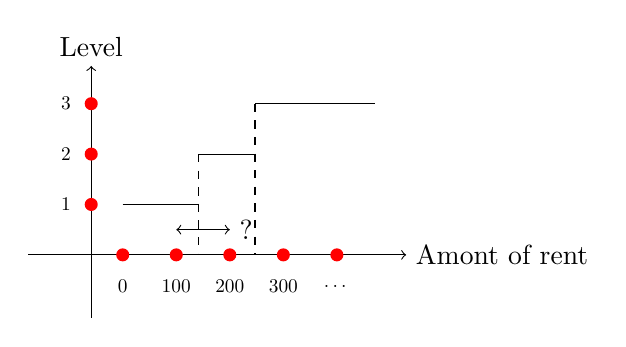
\begin{tikzpicture}[scale=0.8]
      \draw[->] (-1,0) -- (5,0) node[right] {Amont of rent};
      \draw[->] (0,-1) -- (0,3) node[above] {Level};

		\node[scale=0.5,red,circle, fill] (x1) at  (0.5,0) {};
		\node[scale=0.5,red,circle, fill] (x2) at  (1.35,0) {};
		\node[scale=0.5,red,circle, fill] (x3) at  (2.2,0) {};
		\node[scale=0.5,red,circle, fill] (x4) at  (3.05,0) {};
		\node[scale=0.5,red,circle, fill] (x5) at  (3.9,0) {};

		\node[scale=0.7] (x1) at  (0.5,-0.5) {$0$};
		\node[scale=0.7] (x2) at  (1.35,-0.5) {$100$};
		\node[scale=0.7] (x3) at  (2.2,-0.5) {$200$};
		\node[scale=0.7] (x4) at  (3.05,-0.5) {$300$};
		\node[scale=0.7] (x5) at  (3.9,-0.5) {\ldots};


		\node[scale=0.5,red,circle, fill] (x1) at  (0,0.8) {};
		\node[scale=0.5,red,circle, fill] (x2) at  (0,1.6) {};
		\node[scale=0.5,red,circle, fill] (x3) at  (0,2.4) {};

		\node[scale=0.7] (x1) at  (-0.4,0.8) {$1$};
		\node[scale=0.7] (x2) at  (-0.4,1.6) {$2$};
		\node[scale=0.7] (x3) at  (-0.4,2.4) {$3$};

      \draw[-] (0.5,0.8) -- (1.7,0.8);
      \draw[-] (1.7,1.6) -- (2.6,1.6);
      \draw[-] (2.6,2.4) -- (4.5,2.4);

      \draw[dashed] (1.7,1.6) -- (1.7,0);
      \draw[dashed] (2.6,2.4) -- (2.6,0);

      \draw[<-] (1.35,0.4) -- (1.7,0.4);
      \draw[->] (1.7,0.4) -- (2.2,0.4) node[right] {?};

\end{tikzpicture}
\caption{If the admissible quantizations are those displayed in red, and the estimated cutpoints are the dashed lines, which ``rounding'' shall be chosen?}
\label{fig:constraint1}
\end{subfigure}
\begin{subfigure}[t]{0.5\textwidth}
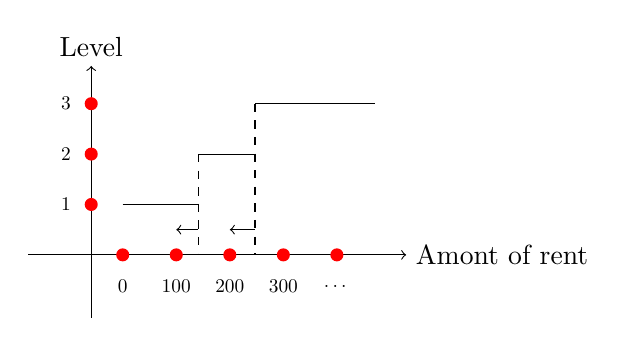
\begin{tikzpicture}[scale=0.8]
      \draw[->] (-1,0) -- (5,0) node[right] {Amont of rent};
      \draw[->] (0,-1) -- (0,3) node[above] {Level};

		\node[scale=0.5,red,circle, fill] (x1) at  (0.5,0) {};
		\node[scale=0.5,red,circle, fill] (x2) at  (1.35,0) {};
		\node[scale=0.5,red,circle, fill] (x3) at  (2.2,0) {};
		\node[scale=0.5,red,circle, fill] (x4) at  (3.05,0) {};
		\node[scale=0.5,red,circle, fill] (x5) at  (3.9,0) {};

		\node[scale=0.7] (x1) at  (0.5,-0.5) {$0$};
		\node[scale=0.7] (x2) at  (1.35,-0.5) {$100$};
		\node[scale=0.7] (x3) at  (2.2,-0.5) {$200$};
		\node[scale=0.7] (x4) at  (3.05,-0.5) {$300$};
		\node[scale=0.7] (x5) at  (3.9,-0.5) {\ldots};


		\node[scale=0.5,red,circle, fill] (x1) at  (0,0.8) {};
		\node[scale=0.5,red,circle, fill] (x2) at  (0,1.6) {};
		\node[scale=0.5,red,circle, fill] (x3) at  (0,2.4) {};

		\node[scale=0.7] (x1) at  (-0.4,0.8) {$1$};
		\node[scale=0.7] (x2) at  (-0.4,1.6) {$2$};
		\node[scale=0.7] (x3) at  (-0.4,2.4) {$3$};

      \draw[-] (0.5,0.8) -- (1.7,0.8);
      \draw[-] (1.7,1.6) -- (2.6,1.6);
      \draw[-] (2.6,2.4) -- (4.5,2.4);

      \draw[dashed] (1.7,1.6) -- (1.7,0);
      \draw[dashed] (2.6,2.4) -- (2.6,0);

      \draw[<-] (1.35,0.4) -- (1.7,0.4);
      \draw[<-] (2.2,0.4) -- (2.6,0.4);

\end{tikzpicture}
\caption{In this setting, rounding has no side effect.}
\label{fig:constraint2}
\end{subfigure}
\begin{subfigure}[t]{0.5\textwidth}
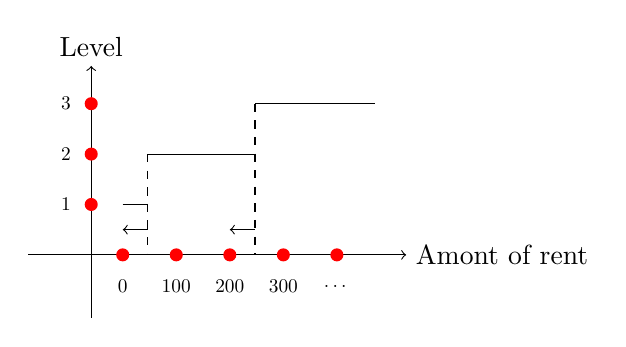
\begin{tikzpicture}[scale=0.8]
      \draw[->] (-1,0) -- (5,0) node[right] {Amont of rent};
      \draw[->] (0,-1) -- (0,3) node[above] {Level};

		\node[scale=0.5,red,circle, fill] (x1) at  (0.5,0) {};
		\node[scale=0.5,red,circle, fill] (x2) at  (1.35,0) {};
		\node[scale=0.5,red,circle, fill] (x3) at  (2.2,0) {};
		\node[scale=0.5,red,circle, fill] (x4) at  (3.05,0) {};
		\node[scale=0.5,red,circle, fill] (x5) at  (3.9,0) {};

		\node[scale=0.7] (x1) at  (0.5,-0.5) {$0$};
		\node[scale=0.7] (x2) at  (1.35,-0.5) {$100$};
		\node[scale=0.7] (x3) at  (2.2,-0.5) {$200$};
		\node[scale=0.7] (x4) at  (3.05,-0.5) {$300$};
		\node[scale=0.7] (x5) at  (3.9,-0.5) {\ldots};


		\node[scale=0.5,red,circle, fill] (x1) at  (0,0.8) {};
		\node[scale=0.5,red,circle, fill] (x2) at  (0,1.6) {};
		\node[scale=0.5,red,circle, fill] (x3) at  (0,2.4) {};

		\node[scale=0.7] (x1) at  (-0.4,0.8) {$1$};
		\node[scale=0.7] (x2) at  (-0.4,1.6) {$2$};
		\node[scale=0.7] (x3) at  (-0.4,2.4) {$3$};

      \draw[-] (0.5,0.8) -- (0.9,0.8);
      \draw[-] (0.9,1.6) -- (2.6,1.6);
      \draw[-] (2.6,2.4) -- (4.5,2.4);

      \draw[dashed] (0.9,1.6) -- (0.9,0);
      \draw[dashed] (2.6,2.4) -- (2.6,0);

      \draw[<-] (0.5,0.4) -- (0.9,0.4);
      \draw[<-] (2.2,0.4) -- (2.6,0.4);

\end{tikzpicture}
\caption{The first level is ``collapsed'' and disappears, with possible consequences to the predictive task.}
\label{fig:constraint3}
\end{subfigure}
\begin{subfigure}[t]{0.5\textwidth}
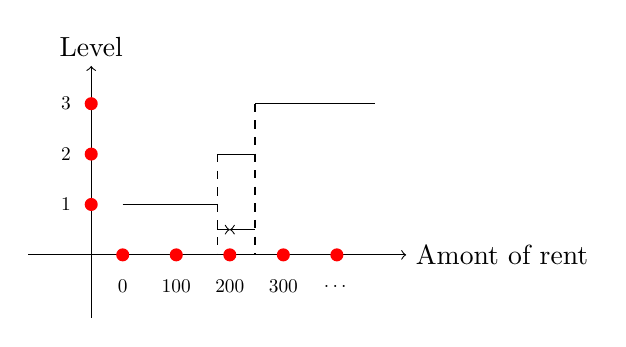
\begin{tikzpicture}[scale=0.8]
      \draw[->] (-1,0) -- (5,0) node[right] {Amont of rent};
      \draw[->] (0,-1) -- (0,3) node[above] {Level};

		\node[scale=0.5,red,circle, fill] (x1) at  (0.5,0) {};
		\node[scale=0.5,red,circle, fill] (x2) at  (1.35,0) {};
		\node[scale=0.5,red,circle, fill] (x3) at  (2.2,0) {};
		\node[scale=0.5,red,circle, fill] (x4) at  (3.05,0) {};
		\node[scale=0.5,red,circle, fill] (x5) at  (3.9,0) {};

		\node[scale=0.7] (x1) at  (0.5,-0.5) {$0$};
		\node[scale=0.7] (x2) at  (1.35,-0.5) {$100$};
		\node[scale=0.7] (x3) at  (2.2,-0.5) {$200$};
		\node[scale=0.7] (x4) at  (3.05,-0.5) {$300$};
		\node[scale=0.7] (x5) at  (3.9,-0.5) {\ldots};


		\node[scale=0.5,red,circle, fill] (x1) at  (0,0.8) {};
		\node[scale=0.5,red,circle, fill] (x2) at  (0,1.6) {};
		\node[scale=0.5,red,circle, fill] (x3) at  (0,2.4) {};

		\node[scale=0.7] (x1) at  (-0.4,0.8) {$1$};
		\node[scale=0.7] (x2) at  (-0.4,1.6) {$2$};
		\node[scale=0.7] (x3) at  (-0.4,2.4) {$3$};

      \draw[-] (0.5,0.8) -- (2,0.8);
      \draw[-] (2,1.6) -- (2.6,1.6);
      \draw[-] (2.6,2.4) -- (4.5,2.4);

      \draw[dashed] (2,1.6) -- (2,0);
      \draw[dashed] (2.6,2.4) -- (2.6,0);

      \draw[<-] (2.2,0.4) -- (2,0.4);
      \draw[<-] (2.2,0.4) -- (2.6,0.4);

\end{tikzpicture}
\caption{The narrow middle level is collapsed, also with possible predictive consequences, since \textit{e.g.}\ rent amounts are often very concentrated around their mean.}
\label{fig:constraint4}
\end{subfigure}
\caption{Different settings of estimated quantizations and the consequences of constraints on the set of admissible cutpoints.}
\label{fig:constraint}
\end{figure}

\subsection{Wrapping up}

Feature quantization (discretization for continuous features, grouping of factor levels for categorical ones) in a supervised multivariate classification setting is a recurring problem in many industrial contexts. This setting was formalized as a highly combinatorial representation learning problem and a new algorithmic approach, named \textit{glmdisc}, has been proposed as a sensible approximation of a classical statistical information criterion.

The first proposed implementation relies on the use of a neural network of particular architecture and specifically a softmax approximation of each discretized or grouped feature. The second proposed implementation relies on an SEM algorithm and a polytomic multiclass \gls{lr} approximation in the same flavor as the softmax. These proposals can alternatively be replaced by any other univariate multiclass predictive model, which make them flexible and adaptable to other problems. Prediction of the target feature, given quantized features, was exemplified with \gls{lr}, although here as well, it can be swapped with any other supervised classification model.

The experiments showed that, as was sensed empirically by statisticians in the field of \textit{Credit Scoring}, discretization and grouping can indeed provide better models than standard \gls{lr}. This novel approach allows practitioners to have a fully automated and statistically well-grounded tool that achieves better performance than \textit{ad hoc} industrial practices at the price of decent computing time but much less of the practitioner's valuable time.

As described in the introduction, \gls{lr} is additive in its inputs which does not allow to take into account conditional dependency, as stated by~\cite{berry2010testing}. This problem is often dealt with by sparsely introducing ``interactions'', \textit{i.e.}\ products of two features. This leads again to a model selection challenge on a highly combinatorial discrete space that could be solved with a similar approach. In a broader context with no restriction on the predictive model, \cite{tsang2018detecting} already made use of neural networks to estimate the presence or absence of statistical interactions. We take another approach in the subsequent chapter where we tackle the parsimonious addition of pairwise interactions among quantized features, that might influence the quantization process introduced in this chapter.

\printbibliography[heading=subbibliography, title=References of Chapter 3]